% Options for packages loaded elsewhere
\PassOptionsToPackage{unicode}{hyperref}
\PassOptionsToPackage{hyphens}{url}
%
\documentclass[
  a4paper,
  oneside,
  openany]{book}
\usepackage{amsmath,amssymb}
\usepackage{lmodern}
\usepackage{iftex}
\ifPDFTeX
  \usepackage[T1]{fontenc}
  \usepackage[utf8]{inputenc}
  \usepackage{textcomp} % provide euro and other symbols
\else % if luatex or xetex
  \usepackage{unicode-math}
  \defaultfontfeatures{Scale=MatchLowercase}
  \defaultfontfeatures[\rmfamily]{Ligatures=TeX,Scale=1}
\fi
% Use upquote if available, for straight quotes in verbatim environments
\IfFileExists{upquote.sty}{\usepackage{upquote}}{}
\IfFileExists{microtype.sty}{% use microtype if available
  \usepackage[]{microtype}
  \UseMicrotypeSet[protrusion]{basicmath} % disable protrusion for tt fonts
}{}
\makeatletter
\@ifundefined{KOMAClassName}{% if non-KOMA class
  \IfFileExists{parskip.sty}{%
    \usepackage{parskip}
  }{% else
    \setlength{\parindent}{0pt}
    \setlength{\parskip}{6pt plus 2pt minus 1pt}}
}{% if KOMA class
  \KOMAoptions{parskip=half}}
\makeatother
\usepackage{xcolor}
\usepackage[top=1in, left=1in, right=1in, bottom=1in]{geometry}
\usepackage{color}
\usepackage{fancyvrb}
\newcommand{\VerbBar}{|}
\newcommand{\VERB}{\Verb[commandchars=\\\{\}]}
\DefineVerbatimEnvironment{Highlighting}{Verbatim}{commandchars=\\\{\}}
% Add ',fontsize=\small' for more characters per line
\usepackage{framed}
\definecolor{shadecolor}{RGB}{248,248,248}
\newenvironment{Shaded}{\begin{snugshade}}{\end{snugshade}}
\newcommand{\AlertTok}[1]{\textcolor[rgb]{0.94,0.16,0.16}{#1}}
\newcommand{\AnnotationTok}[1]{\textcolor[rgb]{0.56,0.35,0.01}{\textbf{\textit{#1}}}}
\newcommand{\AttributeTok}[1]{\textcolor[rgb]{0.77,0.63,0.00}{#1}}
\newcommand{\BaseNTok}[1]{\textcolor[rgb]{0.00,0.00,0.81}{#1}}
\newcommand{\BuiltInTok}[1]{#1}
\newcommand{\CharTok}[1]{\textcolor[rgb]{0.31,0.60,0.02}{#1}}
\newcommand{\CommentTok}[1]{\textcolor[rgb]{0.56,0.35,0.01}{\textit{#1}}}
\newcommand{\CommentVarTok}[1]{\textcolor[rgb]{0.56,0.35,0.01}{\textbf{\textit{#1}}}}
\newcommand{\ConstantTok}[1]{\textcolor[rgb]{0.00,0.00,0.00}{#1}}
\newcommand{\ControlFlowTok}[1]{\textcolor[rgb]{0.13,0.29,0.53}{\textbf{#1}}}
\newcommand{\DataTypeTok}[1]{\textcolor[rgb]{0.13,0.29,0.53}{#1}}
\newcommand{\DecValTok}[1]{\textcolor[rgb]{0.00,0.00,0.81}{#1}}
\newcommand{\DocumentationTok}[1]{\textcolor[rgb]{0.56,0.35,0.01}{\textbf{\textit{#1}}}}
\newcommand{\ErrorTok}[1]{\textcolor[rgb]{0.64,0.00,0.00}{\textbf{#1}}}
\newcommand{\ExtensionTok}[1]{#1}
\newcommand{\FloatTok}[1]{\textcolor[rgb]{0.00,0.00,0.81}{#1}}
\newcommand{\FunctionTok}[1]{\textcolor[rgb]{0.00,0.00,0.00}{#1}}
\newcommand{\ImportTok}[1]{#1}
\newcommand{\InformationTok}[1]{\textcolor[rgb]{0.56,0.35,0.01}{\textbf{\textit{#1}}}}
\newcommand{\KeywordTok}[1]{\textcolor[rgb]{0.13,0.29,0.53}{\textbf{#1}}}
\newcommand{\NormalTok}[1]{#1}
\newcommand{\OperatorTok}[1]{\textcolor[rgb]{0.81,0.36,0.00}{\textbf{#1}}}
\newcommand{\OtherTok}[1]{\textcolor[rgb]{0.56,0.35,0.01}{#1}}
\newcommand{\PreprocessorTok}[1]{\textcolor[rgb]{0.56,0.35,0.01}{\textit{#1}}}
\newcommand{\RegionMarkerTok}[1]{#1}
\newcommand{\SpecialCharTok}[1]{\textcolor[rgb]{0.00,0.00,0.00}{#1}}
\newcommand{\SpecialStringTok}[1]{\textcolor[rgb]{0.31,0.60,0.02}{#1}}
\newcommand{\StringTok}[1]{\textcolor[rgb]{0.31,0.60,0.02}{#1}}
\newcommand{\VariableTok}[1]{\textcolor[rgb]{0.00,0.00,0.00}{#1}}
\newcommand{\VerbatimStringTok}[1]{\textcolor[rgb]{0.31,0.60,0.02}{#1}}
\newcommand{\WarningTok}[1]{\textcolor[rgb]{0.56,0.35,0.01}{\textbf{\textit{#1}}}}
\usepackage{longtable,booktabs,array}
\usepackage{calc} % for calculating minipage widths
% Correct order of tables after \paragraph or \subparagraph
\usepackage{etoolbox}
\makeatletter
\patchcmd\longtable{\par}{\if@noskipsec\mbox{}\fi\par}{}{}
\makeatother
% Allow footnotes in longtable head/foot
\IfFileExists{footnotehyper.sty}{\usepackage{footnotehyper}}{\usepackage{footnote}}
\makesavenoteenv{longtable}
\usepackage{graphicx}
\makeatletter
\def\maxwidth{\ifdim\Gin@nat@width>\linewidth\linewidth\else\Gin@nat@width\fi}
\def\maxheight{\ifdim\Gin@nat@height>\textheight\textheight\else\Gin@nat@height\fi}
\makeatother
% Scale images if necessary, so that they will not overflow the page
% margins by default, and it is still possible to overwrite the defaults
% using explicit options in \includegraphics[width, height, ...]{}
\setkeys{Gin}{width=\maxwidth,height=\maxheight,keepaspectratio}
% Set default figure placement to htbp
\makeatletter
\def\fps@figure{htbp}
\makeatother
\setlength{\emergencystretch}{3em} % prevent overfull lines
\providecommand{\tightlist}{%
  \setlength{\itemsep}{0pt}\setlength{\parskip}{0pt}}
\setcounter{secnumdepth}{5}
\usepackage[utf8]{inputenc}% Usa codificación 8-bit que tiene 256 glyphs
\usepackage[T1]{fontenc}
%Más información de babel : http://www.texnia.com/spanishopt.html
%es-tabla: Traduce table como tabla en lugar de como cuadro.
%es-nodecimaldot: No añade punto tras los números de sección, subsección
\usepackage[spanish,es-nodecimaldot,es-tabla]{babel} 
\usepackage{graphicx} %Manipulación de imágenes : https://es.overleaf.com/learn/latex/Inserting_Images
\usepackage{tikz} % Requerido para dibujar formas personalizadas
\usepackage{float} %Gráficas
\usepackage{fancyhdr} %Para un mejor manejo de encabezados
\usepackage{calc} %Para hacer cálculos matemáticos en Latex
\usepackage{amsmath,amssymb,amsfonts} %Para tener mejores opciones en estructuras matemáticas.
\usepackage{amsthm} %Ambientes matemáticos : http://www.ctex.org/documents/packages/math/amsthdoc.pdf
%Vamos a colocar todo el formato que yihui colocó en su bookdown:https://github.com/rstudio/bookdown/blob/master/inst/examples/latex/preamble.tex
\usepackage{mathrsfs}
\usepackage{booktabs}
\usepackage{longtable}
\renewcommand{\textfraction}{0.05}
\renewcommand{\topfraction}{0.8}
\renewcommand{\bottomfraction}{0.8}
\renewcommand{\floatpagefraction}{0.75}
\usepackage{listings}
\lstset{
  breaklines=true
}
\usepackage{booktabs}
\usepackage{longtable}
\usepackage{array}
\usepackage{multirow}
\usepackage{wrapfig}
\usepackage{float}
\usepackage{colortbl}
\usepackage{pdflscape}
\usepackage{tabu}
\usepackage{threeparttable}
\usepackage{threeparttablex}
\usepackage[normalem]{ulem}
\usepackage{makecell}
\usepackage{xcolor}
\ifLuaTeX
  \usepackage{selnolig}  % disable illegal ligatures
\fi
\usepackage[]{natbib}
\bibliographystyle{apalike}
\nocite{montgomery2021introduction, conover1998practical, gibbons2020nonparametric}
\IfFileExists{bookmark.sty}{\usepackage{bookmark}}{\usepackage{hyperref}}
\IfFileExists{xurl.sty}{\usepackage{xurl}}{} % add URL line breaks if available
\urlstyle{same} % disable monospaced font for URLs
\hypersetup{
  pdftitle={Modelos de Regresión},
  pdfauthor={Sofía Villers Gómez; David Alberto Mateos Montes de Oca; Dulce María Reyes Varela; Carlos Fernando Vásquez Guerra},
  hidelinks,
  pdfcreator={LaTeX via pandoc}}

\title{Modelos de Regresión}
\author{Sofía Villers Gómez \and David Alberto Mateos Montes de Oca \and Dulce María Reyes Varela \and Carlos Fernando Vásquez Guerra}
\date{}

\begin{document}
\maketitle

{
\setcounter{tocdepth}{2}
\tableofcontents
}
\hypertarget{prefacio}{%
\chapter*{Prefacio}\label{prefacio}}


El curso de Modelos No Paramétricos y de Regresión es el segundo curso de estadística en el mapa curricular de la carrera de actuaría en la facultad, por lo que al llegar a este curso es muy probable que ya hayan cursado inferencia estadística en donde se revisan temas de estimación de parámetros (estimación puntual, estimación por interválos, pruebas de hipótesis sobre las estimaciones de dichos parámetros). Se puede notar que las metodologías estudiadas en el curso de inferencia se basan en el supuesto de que conocemos las distribución que sigue nuestra variable de interes y por lo tanto las observaciones provienen de una cierta familia paramétrica de distribuciones y entonces con las observaciones (muestra) podemos hacer inferencia estadística acerca de los valores de los parámetros de dicha distribución.

Sin embargo, hay casos en donde desconocemos la distribución paramétrica de la que provienen nuestros datos y aún así quiseramos poder realizar algún tipo de inferencia sobre la variable de interes o de la población. ¿Se puede?

La respuesta es sí, pero utilizando procedimientos distintos o realizando algunas variaciones a las metodologías vistas en el curso de inferencia estadística. Esos son los temas que se revisan en la primer parte de este curso denominado modelos no paramétricos.

La segunda parte del curso se enfoca en los modelos de regresión lineal, que son modelos estadístico muy usados en diferentes áreas que permiten encontrar relaciones entre 2 variables para el caso simple y entre más de 2 variables en el caso múltiple.

\hypertarget{objetivos}{%
\subsection*{Objetivos}\label{objetivos}}


\begin{itemize}
\item
  Proporcionar a los alumnos el material para cubrir los temas del curso de modelos no paramétricos y de regresión.
\item
  Reforzar las bases teóricas con contenido electrónico completado con herramientas de R-Studio.
\end{itemize}

Este libro fue escrito con \href{http://bookdown.org/}{bookdown} usando \href{http://www.rstudio.com/ide/}{RStudio}.

Esta versión fue escrita con:

\hypertarget{licencia}{%
\subsection*{Licencia}\label{licencia}}


This work is licensed under a \href{https://creativecommons.org/licenses/by-sa/4.0/}{Creative Commons Attribution-ShareAlike 4.0 International License}.

\emph{This is a human-readable summary of (and not a substitute for) the license.
Please see \url{https://creativecommons.org/licenses/by-sa/4.0/legalcode} for the full legal text.}

\textbf{You are free to:}

\begin{itemize}
\item
  \textbf{Share}---copy and redistribute the material in any medium or
  format
\item
  \textbf{Remix}---remix, transform, and build upon the material for any
  purpose, even commercially.
\end{itemize}

The licensor cannot revoke these freedoms as long as you follow the
license terms.

\textbf{Under the following terms:}

\begin{itemize}
\item
  \textbf{Attribution}---You must give appropriate credit, provide a link
  to the license, and indicate if changes were made. You may do so in
  any reasonable manner, but not in any way that suggests the licensor
  endorses you or your use.
\item
  \textbf{ShareAlike}---If you remix, transform, or build upon the material, you must distribute your contributions under the same license as the original.
\item
  \textbf{No additional restrictions}---You may not apply legal terms or
  technological measures that legally restrict others from doing
  anything the license permits.
\end{itemize}

\textbf{Notices:}

You do not have to comply with the license for elements of the
material in the public domain or where your use is permitted by an
applicable exception or limitation.

No warranties are given. The license may not give you all of the
permissions necessary for your intended use. For example, other rights
such as publicity, privacy, or moral rights may limit how you use the
material.

\hypertarget{part-introduccion}{%
\part{Introduccion}\label{part-introduccion}}

\hypertarget{modelos-lineales}{%
\chapter*{Modelos lineales}\label{modelos-lineales}}


Los modelos lineales son una de las herramientas más importantes del análisis cuantitativo. En forma general, estos modelos se utilizan cuando se busca predecir o explicar una variable dependiente a partir de una o más variables independientes. Dependiendo de las características de las variables disponibles, la herramienta estadística más a apropiada para construir el modelo puede variar. Es por esta razón que cuando se construye un modelo estadístico es necesario tener en cuenta los principios de modelización y las caracteristicas de las variables.

\hypertarget{principios-de-la-modelizaciuxf3n-estaduxedstica}{%
\section*{Principios de la modelización estadística}\label{principios-de-la-modelizaciuxf3n-estaduxedstica}}


\begin{itemize}
\item
  Dado un conjunto de variables, cada una de las cuales es un vector de lecturas de un rasgo específico de las muestras en un experimento.
\item
  \textbf{Problema:} ¿De qué manera una variable \(Y\) depende de otras variables \(X_1,...,X_n\) en el estudio?
\item
  Un \textbf{modelo estadístico} define una relación matemática entre los \(X_i\) y \(Y\). El modelo es una representación del real \(Y\) que pretende reemplazarlo en la medida de lo posible. Al menos el modelo debería capturar la dependencia de \(Y\) de los \(X_i\).
\end{itemize}

\hypertarget{identificar-y-caracterizar-variables}{%
\section*{Identificar y Caracterizar Variables}\label{identificar-y-caracterizar-variables}}


Este es el primer paso en el modelado:

\begin{itemize}
\item
  Qué variable es la variable de respuesta;
\item
  Qué variables son las variables explicativas;
\item
  ¿Son las variables explicativas continuas, categóricas o una mezcla de ambas?
\item
  ¿Cuál es la naturaleza de la variable de respuesta? ¿Es una medición contínua, un conteo, una proporción, una categoría o un tiempo hasta un evento?
\end{itemize}

\hypertarget{tipos-de-variables-y-tipo-de-modelo}{%
\section*{Tipos de variables y tipo de modelo}\label{tipos-de-variables-y-tipo-de-modelo}}


\hypertarget{en-funciuxf3n-de-las-variables-explicativas}{%
\subsection*{En función de las variables explicativas}\label{en-funciuxf3n-de-las-variables-explicativas}}


\begin{longtable}[]{@{}
  >{\centering\arraybackslash}p{(\columnwidth - 2\tabcolsep) * \real{0.5810}}
  >{\centering\arraybackslash}p{(\columnwidth - 2\tabcolsep) * \real{0.4190}}@{}}
\toprule()
\begin{minipage}[b]{\linewidth}\centering
Variables Explicativas
\end{minipage} & \begin{minipage}[b]{\linewidth}\centering
Modelo
\end{minipage} \\
\midrule()
\endhead
Todas las variables explicativas continuas & Regresión \\
Todas las variables explicativas categóricas & Análisis de Varianza (ANOVA) \\
Variables explicativas tanto continuas como categóricas & Regresión, Análisis de Covarianza (ANCOVA) \\
\bottomrule()
\end{longtable}

\hypertarget{en-funciuxf3n-de-la-variable-respuesta}{%
\subsection*{En función de la variable respuesta}\label{en-funciuxf3n-de-la-variable-respuesta}}


\begin{longtable}[]{@{}cc@{}}
\toprule()
Variable de respuesta & Tipo de modelo \\
\midrule()
\endhead
Continua & Regresión normal, ANOVA, ANCOVA \\
Proporción & Regresión logística \\
Conteos & Modelo log-lineal (regresión Poisson) \\
Binario & Regresión logística binaria \\
Tiempo hasta evento & Análisis de supervivencia \\
\bottomrule()
\end{longtable}

\hypertarget{el-modelo-lineal-general}{%
\section*{El modelo lineal general}\label{el-modelo-lineal-general}}


Como se mencionó, un modelo lineal, es un modelo para el \textbf{análisis de regresión}, que tiene como objetivo determinar una función matemática que describa el comportamiento de una variable dados los valores de otra u otras variables.

En particular el \textbf{análisis de regresión simple}, pretende estudiar y explicar el comportamiento de una variable que notamos \(y\), y que llamaremos \textbf{variable respuesta}, \textbf{variable dependiente} o \textbf{variable de interés}, a partir de otra variable, que notamos \(x\), y que llamamos \textbf{variable explicativa}, \textbf{variable independiente}, \textbf{covariable} o \textbf{regresor}.

El principal objetivo de la regresión es encontrar la función que mejor explique la relación entre la variable dependiente y las independientes.

\begin{itemize}
\tightlist
\item
  Una forma muy general para el modelo sería
\end{itemize}

\[
      y = f(x_1,x_2,...,x_p) + \epsilon,
\]

donde \(f\) es una función desconocida y \(\epsilon\) es el error en esta representación.
Puesto que normalmente no tenemos suficientes datos para intentar estimar \(f\) directamente, normalmente tenemos que asumir que tiene alguna forma restringida.

\begin{itemize}
\tightlist
\item
  La forma más simple y común es el \textbf{modelo lineal (LM)}.
\end{itemize}

\[
    y = \beta_0 + \beta_1 x_1 + \beta_2 x_z + \epsilon,
\]

donde \(\beta_i\) \(i=0,1,2\) son parámetros \emph{desconocidos}.

\(\beta_0\) se llama el término de intercepción. Por lo tanto, el problema se reduce a la estimación de cuatro valores en lugar de los complicados e infinitos \(f\) dimensionales.

\begin{itemize}
\tightlist
\item
  Un modelo lineal simple con una sola variable exploratoria se define como:
\end{itemize}

\[
         \hat{y} = \hat{\beta}_0 + \hat{\beta}_1 x
\]

donde \(\hat y\) son los valores ajustados para \(\hat{\beta}_0\) (intercepto) y \(\hat{\beta}_1\) (pendiente). Luego por un \(x_i\) dado obtenemos un \(\hat{y}_i\) que se aproxima a \(y_i\).

Es posible apreciar que el tema de modelos lineales es bastante amplio y en este curso sólo nos enfocaremos en los modelos de regresión normal múltiple, análisis de varianza y modelos dinámicos.

\hypertarget{part-regresiuxf3n-lineal-simple}{%
\part{Regresión Lineal Simple}\label{part-regresiuxf3n-lineal-simple}}

\hypertarget{introducciuxf3n}{%
\chapter*{Introducción}\label{introducciuxf3n}}


Los primeros problemas prácticos tipo regresión iniciaron en el siglo XVIII, relacionados con la navegación basada en la Astronomía.
Legendre desarrolló el método de mínimo cuadrados en 1805. Gauss afirma que él desarrolló este método algunos años antes y demuestra, en 1809, que mínimos cuadrados proporciona una solución óptima cuando los errores se distribuyen normal. Francis Galton acuña el término regresión al utilizar el modelo para explicar el fenómeno de que los hijos de padres altos, tienden a ser altos en su generación, pero no tan altos como lo fueron sus padres en la propia, por lo que hay un efecto de \emph{regresión}.

El modelo de regresión lineal es, probablemente, el modelo de su tipo más conocido en estadística.

El modelo de regresión se usa para explicar o modelar la relación entre una sola variable, \(y\), llamada dependiente o respuesta, y una o más variables predictoras, independientes, covariables, o explicativas, \(x_1, x_2, ..., x_p\). Si \(p = 1\), se trata de un modelo de regresión simple y si \(p > 1\), de un modelo de regresión múltiple. En este modelo se asume que la variable de respuesta, \(y\), es aleatoria y las variables explicativas son fijas, es decir, no aleatorias.

La variable de respuesta debe ser continua, pero los regresores pueden tener cualquier escala de medición.

\hypertarget{objetivos-del-anuxe1lisis-de-regresiuxf3n}{%
\section*{Objetivos del análisis de regresión}\label{objetivos-del-anuxe1lisis-de-regresiuxf3n}}


Existen varios objetivos dentro del análisis de regresión, entre otros:

\begin{itemize}
\tightlist
\item
  Determinar el efecto, o relación, entre las variables explicativas y la respuesta.
\item
  Predicción de una observación futura.
\item
  Describir de manera general la estructura de los datos.
\end{itemize}

\hypertarget{el-algoruxedtmo-de-regresiuxf3n-lineal}{%
\section*{El algorítmo de regresión lineal}\label{el-algoruxedtmo-de-regresiuxf3n-lineal}}


Sea \(\Phi: \mathcal{X} \rightarrow \mathbb{R}^N\) y consideremos la familia de hipótesis lineales \[H=\{x\mapsto w \cdot \Phi(x)+b | w\in\mathbb{R}^N, b\in\mathbb{R}\}\]

La regresión lineal consiste en buscar la hipótesis \(h\in H\) con el menor error cuadrático medio, es decir, se debe resolver el problema de optimización: \[\min \frac{1}{m}\sum_{i=1}^{m}(h(x_i)-y_i)^2\]

\hypertarget{regresiuxf3n-lineal-simple}{%
\section*{Regresión lineal simple}\label{regresiuxf3n-lineal-simple}}


\begin{center}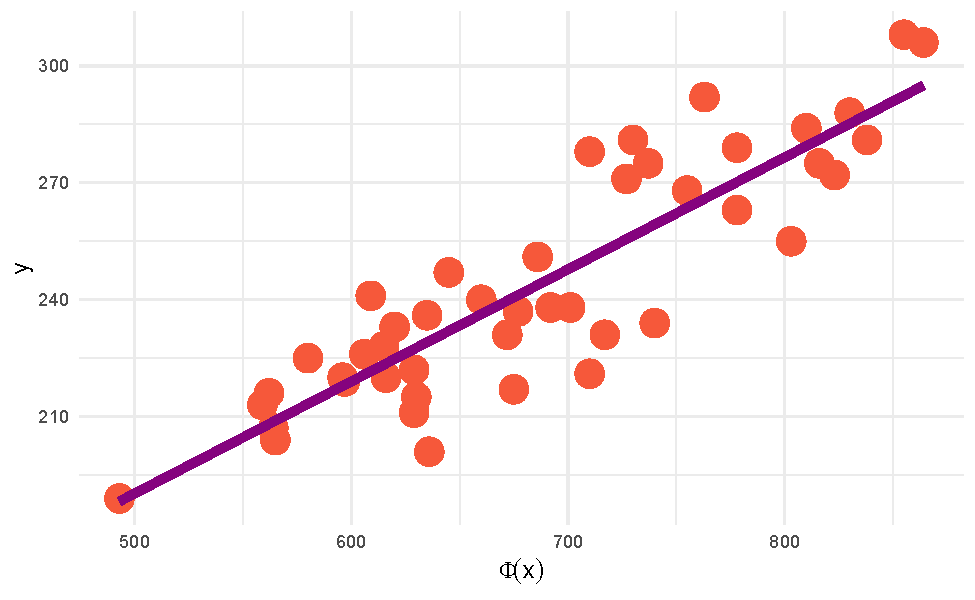
\includegraphics{_main_files/figure-latex/unnamed-chunk-3-1} \end{center}

Para este modelo supondremos que nuestra respuesta, \(y\), es explicada únicamente por una covariable, \(x\).

Entonces, escribimos nuestro modelo como:

\[y^{(i)}=\beta_0+\beta_1x^{(i)}+\epsilon^{(i)},\ \ i=1,2,\dots,n\]
Como podemos observar, se ha propuesto una relación lineal entre la variable \(y\) y la variable explicativa \(x\), que es nuestro primer supuesto sobre el modelo: La relación funcional entre \(x\) y \(y\) es una línea recta.

Observamos que la relación no es perfecta, ya que se agrega el término de error, \(\epsilon\). Dado que la parte aleatoria del modelo es la variable \(y\), asumimos que al error se le ``cargan'' los errores de medición de \(y\), así como las perturbaciones que le pudieran ocasionar los términos omitidos en el modelo.
Gauss desarrolló este modelo a partir de la teoría de errores de medición, que es de donde se desprenden los supuestos sobre este término:

\begin{itemize}
\tightlist
\item
  \(\mathbb{E}(\epsilon^{(i)})=0\)
\item
  \(\mathbb{V}ar(\epsilon^{(i)})=\sigma^2\)
\item
  \(\mathbb{C}ov(\epsilon^{(i)},\epsilon^{(j)})=0, \ \forall i\neq j\)
\end{itemize}

NOTA: Los errores \(\epsilon^{(i)}\) son variables aleatorias no observables.

\hypertarget{modelo-con-intercepto}{%
\chapter{Modelo con intercepto}\label{modelo-con-intercepto}}

El objetivo principal del \textbf{Modelo de Regresión Lineal Simple} es el poder asociar o ajustar a una dispersión de datos una función (en primera instancia se abordará el ajuste mediante una recta) cuyos parámetros dependan directamente de las observaciones con la finalidad de poder resumir, simplificar u obtener propiedades importantes sobre comportamiento de la muestra.

Dicho modelo es el más sencillo de los modelos lineales e involucra una variable de interés \(y\) llamada \textbf{dependiente} o \textbf{respuesta} y su relación con la variable \textbf{predictoria} o \textbf{independiente} \(x\), estableciendo que la media de la variable dependiente \(y\) cambia a razón constante cuando el valor de la variable independiente \(x\) crece o decrece.

El modelo de regresión lineal simple en general es:

\[y_{i}=\beta_{0}+\beta_{1}x_{i}+\epsilon_{i},\]
donde:

\begin{itemize}
\item
  x es la variable regresora,
\item
  y es la variable de respuesta,
\item
  \(\beta_{0}\) ordenada al origen,
\item
  \(\beta_{1}\) pendiente del modelo,
\item
  \(\epsilon\) es un error aleatorio.
\end{itemize}

Conviene considerar a la variable regresora \(x\) como una varible determinista, o bien, una variable controlada por el investigador la cual puede ser medida, mientras que la variable respuesta \(y\) es una variable aleatoria. Ahora bien, los datos no caen exactamente sobre una recta por lo que se considera \(\epsilon\) como un error estadístico, esto es, que es una variable aleatoria que explica por qué el modelo no ajusta exactamente los datos.

Una vez vista la ecuación general del modelo de regresión lineal simple se hablará de algunos supuestos que se deben de cumplir al ajustar una serie de datos, éstas consideraciones hace que en ocaciones carezca de sentido realizar una regresión lineal, sin embargo, no hay que perder de vista que éste es un modelado por lo que algunas características físicas del problema pueden haber sido simplificadas u omitidas.

\textbf{Definición 2.1} (Supuestos del Modelo de Regresión Simple).

En el modelo de regresión simple se supone que \(\epsilon\) satisface:

\begin{itemize}
\item
  \(\mathbf{E}[\epsilon_{i}]=0\)
\item
  \(\textbf{Var}(\epsilon_{i})=\sigma^2\)
\item
  \(\textbf{Cov}(\epsilon_{i},\epsilon_{j})= 0 \  \ \ \forall \ i = 1, \ldots, n, \ \  j=1, \ldots, n, \ \  i \neq j.\)
\item
  \(\epsilon \sim N(0,\sigma^2)\)
\end{itemize}

Una vez considerados estos supuestos se pueden obtener resultados aún más importantes.

Por ejemplo, con los supuestos dados es posible calcular la esperanza y la varianza de la variable \(y_{i}\), dado un valor \(x_{i}\).

\textbf{Teorema 2.1} Sea \(y\) una variable de interés, denominada variable de respuesta, la cual es relacionada con una variable regresora \(x\), entonces:

\textbf{a)} \(\mathbf{E}[y_{i}]=\beta_{0}+\beta_{1}x_{i}\)

\textbf{b)} \(\textbf{Var}(y_{i})=\sigma^2\)

\textbf{Demostración:}

\textbf{a)}

\[\mathbf{E}[y_{i}]=\mathbf{E}[\beta_{0}+\beta_{1}x_{i}+\epsilon_{i}]\]

La parte aleatoria de \(y_{i}\) es \(\epsilon_{i}\); ~ \(\beta_{0}\),\(\beta_{1}\) son constantes y \(x_{i}\) ya es un valor dado; por lo que:

\[\mathbf{E}[y_{i}]=\beta_{0}+\beta_{1}x_{i}+\mathbf{E}[\epsilon_{i}]\]

\[=\beta_{0}+\beta_{1}x_{i}+0\]
\[\therefore \mathbf{E}[y_{i}]=\beta_{0}+\beta_{1}x_{i}.\]
\textbf{b)}

\[Var(y_{i})= Var(\beta_{0}+\beta_{1}x_{i}+\epsilon{i})\]
La parte aleatoria de \(y_{i}\) es \(\epsilon_{i}\); \(\beta_{0}\),\(\beta_{1}\) son constantes y \(x_{i}\) ya es un valor dado; por lo que \(Var(c+\epsilon_{i})=Var(\epsilon_{i})\) con \(c\) constante, de esta manera:

\[Var(y_{i})=0+0+Var(\epsilon_{i})\]
\[\therefore Var(y_{i})=\sigma^2\]

\hypertarget{estimaciuxf3n-por-muxednimos-cuadrados-de-los-paruxe1metros-del-modelo}{%
\section{Estimación por mínimos cuadrados de los parámetros del modelo}\label{estimaciuxf3n-por-muxednimos-cuadrados-de-los-paruxe1metros-del-modelo}}

El modelo de regresión lineal simple

\[y=\beta_{0}+\beta_{1}x+\epsilon\]

cuenta con dos parámetros desconocidos, \(\beta_{0}\) y \(\beta_{1}\), los cuales deben ser estimados a partir de los datos de la muestra. Con la hipótesis de varianza constante sobre los errores, aparece otro parámetro \(\sigma^2\) desconocido, aunque no está incluido en el modelo también debe ser estimado.
Un procedimiento para estimar los parámetros de un modelo lineal simple es el \textbf{método de mínimos cuadrados}, que se puede ilustar sencillamente aplicándolo para ajustar una línea recta a \((x_{1},y_{1}),(x_{2},y_{2}),\ldots,(x_{n},y_{n})\), se estiman \(\beta_{0}\) y \(\beta_{1}\) tales que la suma de los cuadrados de las diferencias entre las observaciones \(y_{i}\) y la línea recta sea mínima.

\textbf{Definición 2.2} (Residuos). Sea \(y_{i}\) los valores observados, \(\hat{y_{i}}\) los valores estimados mediante la regresión lineal simple. La forma de calcular la desviación de \(y_{i}\) con respecto a su media estimada \(\hat{y_{i}}=\hat{\beta_{0}}+\hat{\beta_{1}}x_{i}\) para un \(\hat{\beta_{0}}\) y \(\hat{\beta_{1}}\) dados es:

\[e_{i}=y_{i}-\hat{y_{i}}\]
donde \(e_{i}\) son los residuos.

Por lo anterior,

\[e_{i}=y_{i}-\hat{\beta_{0}}-\hat{\beta_{1}}x_{i}\]
Como se mencionó, lo que se busca es que la diferencia entre todos los valores observados y los valores estimados sea 0, es decir, que la suma de distancias entre \(y_{i}\) y \(\hat{y_{i}}\) sea cero, lo anterior significa que:

\[\sum_{i=1}^{n}e_{i}=0\]
Para estimar \(\beta_{0}\) y \(\beta_{1}\) el \textbf{método de mínimos cuadrados} propone minimizar la suma de los cuadrados de los residuos, ya que de ésta manera se minimizan las distancias verticales entre las observaciones reales \((y)\) y las estimadas \((\hat{y})\), ya que entre más cercanas a cero se encuentren las distancias, mejor se ajusta el modelo a los datos.
Antes de continuar, es necesario abordar unos cuantos resultados.

Se define a:

\[S_{xx}=\sum_{i=1}^{n}(x_{i}-\overline{x})^{2}\]
\[=\sum_{i=1}^{n}(x_{i}^2-2x_{i}\overline{x}+\overline{x}_{i}^{2})\]
\[=\sum_{i=1}^{n}x_{i}^{2}-\sum_{i=1}^{n}2x_{i}\overline{x}+\sum_{i=1}^{n}\overline{x}_{i}^2\]
\[=\sum_{i=1}^{n}x_{i}^2-2\overline{x}^2n+\overline{x}_{i}^2n\]

\[S_{xx}=\sum_{i=1}^{n}x_{i}^2-\overline{x}^2n.\]

También definimos:

\[S_{xy}=\sum_{i=1}^{n}(xi-\overline{x})(y_{i}-\overline{y})\]

\[=\sum_{i=1}^{n}(x_{i}-\overline{x})y_{i}\]

\[=\sum_{i=1}^{n}x_{i}(y_{i}-\overline{y})\]
\[=\sum_{i=1}^{n}X_{i}y_{i}-\left(\sum_{i=1}^{n}x_{i}\right) \left(\sum_{i=1}^{n}y_{i}\right) \ /{n}\]

\[S_{xy}=\sum_{i=1}^{n}x_{i}y_{i}-n\overline{x}\overline{y}\]

Una vez definida la notación, tenemos el siguiente teorema:

\textbf{Teorema 2.2} (Mínimos Cuadrados). Sea \(\hat{\beta_0}\) y \(\hat{\beta_{1}}\) los parámetros que minimizan la suma de cuadrados de la diferencia entre los valores observados y los estimados \(\left(\sum_{i=1}^{n}e_i^2\right)\) entonces:

\textbf{a)} \(\hat{\beta_{0}}=\overline{y}-\hat{\beta_{1}}\overline{x}\)

\textbf{b)} \(\hat{\beta_{1}}=\frac{S_{xy}}{S_{xx}}=\frac{\sum_{i=1}^{n}(x_{i}-\overline{x})(y_{i}-\overline{y})}{\sum_{i=1}^{n}(x_{i}-\overline{x})^2}\)

\textbf{Demostración:}

\textbf{a)}

Tenemos:

\[\sum_{i=1}^{n}e_{i}^2=\sum_{i=1}^{n}(y_{i}-\hat{\beta_{0}}-\hat{\beta_{1}}x_{i})^2.\]
Minimizando la suma de cuadrados, se deriva respecto a \(\hat{\beta_{0}}\)

\[\frac{\delta\sum_{i=1}^{n}e_{i}^2}{\delta\hat{\beta_{0}}}=-2\sum_{i=1}^{n}(y_{i}-\hat{\beta_{0}}-\hat{\beta_{1}}x_{i})\]
\[\frac{\delta\sum_{i=1}^{n}e_{i}^2}{\delta\hat{\beta_{0}}}=-2\left(\sum_{i=1}^{n}y_{i}-\sum_{i=1}^{n}\hat{\beta_{0}}-\sum_{i=1}^{n}\hat{\beta_{1}x_{i}}\right).\]
Igualando a 0

\[-2\left(\sum_{i=1}^{n}y_{i}-\hat{\beta_{0}}n-\sum_{i=1}^{n}\hat{\beta_{1}}x_{i}\right)=0\]
\[\sum_{i=1}^{n}y_{i}-\hat{\beta_{0}}n-\sum_{i=1}^{n}\hat{\beta_{1}}x_{i}=0\]
\[\sum_{i=1}^{n}y_{i}=n\hat{\beta_{0}}+\hat{\beta_{1}}\sum_{i=1}^{n}x_{i}\]
\[\overline{y}n=n\hat{\beta_{0}}+\hat{\beta_{1}}\overline{x}n\]
\[\overline{y}=\hat{\beta_{0}}+\hat{\beta_{1}}\overline{x}\]
\[\therefore\hat{\beta_{0}}=\overline{y}-\hat{\beta_{1}}\overline{x}.\blacksquare\]
Por lo tanto se obtiene el primer estimador, \(\hat{\beta_{0}}\); para el estimador de \(\beta_{1}\) se deriva respecto a \(\hat{\beta_{1}}\):

\[\frac{\delta\sum_{i=1}^{n}e_{i}^2}{\delta\hat{\beta_{1}}}=-2\sum_{i=1}^{n}(y_{i}-\hat{\beta_{0}}-\hat{\beta_{1}}x_{i})x_{i}\]
\[=-2\left(\sum_{i=1}^{n}x_{i}y_{i}-\sum_{i=1}^{n}\hat{\beta_{0}}x_{i}-\sum_{i=1}^{n}\hat{\beta_{1}}x_{i}^2\right).\]
Igualando la derivada a 0 para hallar el punto crítico

\[-2\left(\sum_{i=1}^{n}x_{i}y_{i}-\sum_{i=1}^{n}\hat{\beta_{0}}x_{i}-\sum_{i=1}^{n}\hat{\beta_{1}}x_{i}^2\right)=0\]

\[\sum_{i=1}^{n}x_{i}y_{i}-\sum_{i=1}^{n}\hat{\beta_{0}}x_{i}-\sum_{i=1}^{n}\hat{\beta_{1}}x_{i}^2=0\]
\[\sum_{i=1}^{n}x_{i}y_{i}=\sum_{i=1}^{n}\hat{\beta_{0}}x_{i}+\sum_{i=1}^{n}\hat{\beta_{1}}x_{i}^2\]
\[\sum_{i=1}^{n}x_{i}y_{i}=\hat{\beta_{0}}\sum_{i=1}^{n}x_{i}+\hat{\beta_{1}}\sum_{i=1}^{n}x_{i}^2\]
\[\sum_{i=1}^{n}x_{i}y_{i}=\hat{\beta_{0}}\overline{x}n+\hat{\beta_{1}}\sum_{i=1}^{n}x_{i}^2\]
Sustituyendo \(\hat{\beta_{0}}\) por \(\overline{y}-\hat{\beta_{1}}\overline{x}\) se tiene:

\[\sum_{i=1}^{n}x_{i}y_{i}=\overline{y}\overline{x}n-\hat{\beta_{1}}\overline{x}^2n+\hat{\beta_{1}}\sum_{i=1}^{n}x_{i}^2\]
\[\sum_{i=1}^{n}x_{i}y_{i}-\overline{y}\overline{x}n+\hat{\beta_{1}}\overline{x}^2n-\hat{\beta_{1}}\sum_{i=1}^{n}x_{i}^2\]
Por la notación tenemos que: \(S_{xy}=\sum x_{i}y_{i} - n \overline{x}\overline{y}\) y \(S_{xx}= \sum x_{i}^2 - n\overline{x}^2\)

\[\frac{\delta \sum_{i=1}^{n}e_{i}^2}{\delta\hat{\beta_{1}}}=-2\left(S_{xy}-\hat{\beta_{1}\left(\sum_{i=1}^{n}x_{i}^2-\overline{x}^2n\right)}\right)\]
\[=-2(S_{xy}-\hat{\beta_{1}}S_{xx}).\]
Igualando a 0

\[-2(S_{xy}-\hat{\beta_{1}}S_{xx})=0\]
\[S_{xy}-\hat{\beta_{1}}S_{xx}=0\]
\[\Rightarrow \hat{\beta_{1}}=\frac{S_{xy}}{S_{xx}}\]
\[\therefore \hat{\beta_{1}}=\frac{\sum_{i=1}^{n}(x_{i}-\overline{x})(y_{i}-\overline{y})}{\sum_{i=1}^{n}(x_{i}-\overline{x})^2}.\blacksquare\]
De esta manera se demuestra el teorema 2.2. Un punto a destacar es que las siguientes ecuaciones:

\[
\left\{
\begin{array}{ll} \hat{\beta_{0}} \ \ n  \ \ \  \ \ \ \ \ \ + \ \hat{\beta_{1}}\sum_{i=1}^{n}x_{i}\  \ = \ \sum_{i=1}^{n}y_{i} \\
\\
\hat{\beta_{0}} \ \sum_{i=1}^{n}x_{i} \ + \ \hat{\beta_{1}}\sum_{i=1}^{n}x_{i}^2 \ \ = \ \sum_{i=1}^{n}x_{i}y_{i}
\end{array}
\right. 
\]

Son conocidas como las \textbf{ecuaciones normales}, que en conjunto forman un sistema de ecuaciones; al resolverlas simultáneamente para \(\hat{\beta_{0}}\) y \(\hat{\beta_{1}}\) se obtiene los estimadores de \(\beta_{0}\) y \(\beta_{1}\) que se plantean en el teorema anterior.

Un problema del método de mínimos cuadrados es que no proporciona un estimador para \(\sigma^2\), sin embargo, se obtendrá bajo el supuesto de normalidad que es el siguiente:

\[\hat{\sigma}^2=\frac{1}{n-2}\sum_{i=1}^{n}(y_{i}-\hat{y_{i}})^2\]
De esta manera se ha cumplido el objetivo que se planteó al inicio, encontrar los estimadores de \(\beta_{0}\) y \(\beta_{1}\) tal que los residuales fueran igual a 0.

\textbf{Teorema 2.3} (Diferencia de Residuales) Sea \(\hat{\beta_{0}}\) y \(\hat{\beta_{1}}\) los estimadores de mínimos cuadrados de \(\beta_{0}\) y \(\beta_{1}\), respectivamente, entonces la suma de las distancias entre \(y_{i}\) y \(\hat{y_{i}}\) es cero, es decir:

\[\sum_{i=1}^{n}e_{i}=0\]

\textbf{Demostración}

Tenemos que el residual \(e_{i}\) se calcula como: \(e_{i}=y_{i}-\hat{\beta_{0}}-\hat{\beta_1}x_{i}\) entonces si sustituimos se tiene:

\[\sum_{i=1}^{n}e_{i}=\sum_{i=1}^{n}\left(y_{i}-\hat{\beta_{0}}-\hat{\beta_1}x_{i}\right)\]

\[=\sum_{i=1}^{n}y_{i}-\sum_{i=1}^{n}\hat{\beta_{0}}-\sum_{i=1}^{n}\hat{\beta_{1}}x_{i}\]
\[=n\overline{y}-n\hat{\beta_{0}}-n\hat{\beta_{1}}\overline{x}\]
\[=n\left[\overline{y}-\hat{\beta_{0}}-\hat{\beta_{1}}\overline{x}\right]\]
Recordando que la estimación de \(\hat{\beta_{0}}=\overline{y}-\hat{\beta_{1}}\overline{x}\) tenemos:

\[=n\left[\overline{y}-\overline{y}+\hat{\beta_{1}}\overline{x}-\hat{\beta_{1}}\overline{x}\right]\]

\(\therefore \sum_{i=1}^{n}e_{i}=0. \blacksquare\)

Esto implica que si la suma de residuales es 0, entonces la \(\sum_{i=1}^{n}\hat{y_{i}}=\sum_{i=1}^{n}y_{i}\) y vamos a demostrarlo:

\textbf{Corolario 1} Sea \(\hat{\beta_{0}}\) y \(\hat{\beta_{1}}\) los estimadores de mínimos cuadrados de \(\beta_{0}\) y \(\beta_{1}\) respectivamente, si se cumple el teorema anterior, entonces la suma de los valores observados y la suma de los valores ajustados por la regresión son iguales, es decir:

\[\sum_{i=1}^{n}\hat{y_{i}}=\sum_{i=1}^{n}y_{i}\]

\textbf{Demostración}

Por definición:

\[\sum_{i=1}^{n}\hat{y_{i}}=\sum_{i=1}^{n}\left(\hat{\beta_{0}}+\hat{\beta_{1}}x_{i}\right)\]
Por la estimación de \(\hat{\beta_{1}}\)

\[=\sum_{i=1}^{n}\left(\overline{y}-\hat{\beta_{1}}\overline{x}+\hat{\beta_{1}}x_{i}\right)\]
\[=\sum_{i=1}^{n}\overline{y}-n\hat{\beta_{1}}\overline{x}+\hat{\beta_{1}}\sum_{i=1}^{n}x_{i}\]
\[=n\overline{y}-n\hat{\beta_{1}}\overline{x}+n\hat{\beta_{1}}\overline{x}\]
\[=n\overline{y}\]
Por construcción de \(\overline{y}\)

\[\therefore \sum_{i=1}^{n}\hat{y_{i}}=\sum_{i=1}^{n}y_{i}. \blacksquare\]

Una consecuencia de lo anterior,

\textbf{Corolario 2} Sea \(\hat{y_{i}}\) el valor estimado de la forma ~ \(\hat{y_{i}}=\hat{\beta_{0}}+\hat{\beta_{1}}x_{i}\) ~ y el residual ~\(e_{i}=y_{i}-\hat{y_{i}}\), entonces se cumple que:

\[\sum_{i=1}^{n}\hat{y_{i}}e_{i}=0\]

\textbf{Demostración}

Por definición de las \(\hat{y}\)

\[\sum_{i=1}^{n}\hat{y_{i}}e_{i}=\sum_{i=1}^{n}(\hat{\beta_{0}}+\hat{\beta_{1}}x_{i})e_{i}\]
\[=\sum_{i=1}^{n}\left(\hat{\beta_{0}}e_{i}+\hat{\beta_{1}}x_{i}e_{i}\right)\]

\[=\sum_{i=1}^{n}\hat{\beta_{0}}e_{i}+\sum_{i=1}^{n}\hat{\beta_{1}}x_{i}e_{i}\]
\[=\hat{\beta_{0}}\sum_{i=1}^{n}e_{i}+\hat{\beta_{1}}\sum_{i=1}^{n}x_{i}e_{i}\]
Y como demostramos anteriormente, la suma de los residuos es cero:

\[=\hat{\beta_{1}}\sum_{i=1}^{n}x_{i}(y_{i}-\hat{y_{i}})\]
\[=\hat{\beta_{1}}\sum_{i=1}^{n}\left(x_{i}y_{i}-x_{i}\hat{\beta_{0}}-x_{i}^{2}\hat{\beta_{1}}\right)\]
\[=\hat{\beta_{1}}\sum_{i=1}^{n}\left(x_{i}y_{i}-x_{i}^2\hat{\beta_{1}}-x_{i}y_{i}+x_{i}^{2}\hat{\beta_{1}}\right)\]

Entonces:

\[\sum_{i=1}^{n}\hat{y_{i}}e_{i}=0. \blacksquare\]

\hypertarget{propiedades-de-los-estimadores}{%
\section{Propiedades de los estimadores}\label{propiedades-de-los-estimadores}}

Los estimadores \(\hat{\beta_{0}}\) y \(\hat{\beta_{1}}\) tienen propiedades estadísticas muy importantes. ya que son estimadores insesgados, además son de mínima varianza. La propiedad de insesgamiento se revisará en el siguiente teorema:

\textbf{Teorema 2.4} Sea \(\hat{\beta_{0}}\), \(\hat{\beta_{1}}\) los estimadores de mínimos cuadrados de \(\beta_{0}\) y \(\beta_{1}\), respectivamente, entonces los estimadores \(\hat{\beta_{0}}\),\(\hat{\beta_{1}}\) son insesgados. Es decir:

\textbf{a)} \(\mathbf{E}\left[\hat{\beta_{1}}\right]=\beta_{1}\)

\textbf{b)} \(\mathbf{E}\left[\hat{\beta_{0}}\right]=\beta_{0}\)

\textbf{Demostración}

\textbf{a)} Para demostrar el insesgamiento de \(\hat{\beta_{1}}\) usaremos la propiedad de combinación lineal de \(\beta_{1}:\)

``Haremos un pequeño paréntesis para demostrarlo''

Tenemos:

\[\hat{\beta_{1}}=\frac{S_{xy}}{S_{xx}}\]
Sustituyendo \(S_{xx}\) y \(S_{xy}\)

\[\hat{\beta_{1}}=\frac{\sum_{i=1}^{n}(x_{i}-\overline{x})y_{i}}{S_{xx}}\]
\[=\sum_{i=1}^{n}\left(\frac{x_{i}-\overline{x}}{S_{xx}}\right)y_{i}.\]
Haciendo \(a=\frac{(x_{i}-\overline{x})}{S_{xx}}\) nada depende de \(y\), por lo que \(a\) es constante, por consiguiente la combinación lineal de las \(y_{i}\) para \(\hat{\beta_{1}}\) es:

\[\therefore \hat{\beta_{1}}=\sum_{i=1}^{n}ay_{i}.\]
Para la combinación lineal de las \(y_{i}\) para \(\hat{\beta_{0}}\) se tiene:

\[\hat{\beta_{0}}=\overline{y}-\hat{\beta_{1}}\overline{x}\]
Sustituyendo la combinación lineal de \(\hat{\beta_{1}}\) y notación de \(S_{xx}\)

\[\hat{\beta_{0}}=\sum_{i=1}^{n}\frac{y_{i}}{n}-ay_{i}\overline{x}\]
\[=\sum_{i=1}^{n}(\frac{1}{n}-a\overline{x})y_{i}\]
\[=\sum_{i=1}^{n}\left(\frac{1}{n}-\left(\frac{(x_{i}-\overline{x})}{S_{xx}}\right)\overline{x}\right)y_{i}. \]
Haciendo \(b=\frac{1}{n}-\left(\frac{(x_{i}-\overline{x})}{S_{xx}}\right)\overline{x}\) nada depende de \(y\), por lo que \(b\) es constante, entonces la combinación lineal de \(y_{i}\) para \(\hat{\beta_{0}}\) es:

\[\therefore \hat{\beta_{0}}=\sum_{i=1}^{n}by_{i}.\]

``Regresando del paréntesis tenemos:''

\[\mathbf{E}\left[\hat{\beta_{1}}\right]=\mathbf{E}\left[\sum_{i=1}^{n}ay_{i}\right]\]
\[=\sum_{i=1}^{n}a\mathbf{E}[y_{i}].\]
Tenemos que \(\mathbf{E}[y_{i}]=\beta_{0}+\beta_{1}x_{i}\), sustituyendo:

\[\mathbf{E}\left[\hat{\beta_{1}}\right]=\sum_{i=1}^{n}a(\beta_{0}+\beta_{1}x_{i})\]
\[=\sum_{i=1}^{n}a\beta_{0}+\sum_{i=1}^{n}a\beta_{1}x_{i}\]
\[=\beta_{0}\sum_{i=1}^{n}a+\beta_{1}\sum_{i=1}^{n}ax_{i}.\]
Sustituyendo \(a\) de la linealidad de \(\beta_{1}\) se tiene:

\[\mathbf{E}\left[\hat{\beta_{1}}\right]=\beta_{0}\sum_{i=1}^{n}\left(\frac{(x_{i}-\overline{x})}{S_{xx}}\right)+\beta_{1}\sum_{i=1}^{n}\left(\frac{(x_{i}-\overline{x})}{S_{xx}}\right)x_{i}\]
\[=\frac{\beta_{0}}{S_{xx}}(n\overline{x}-\overline{x}n)+\frac{\beta_{1}}{S_{xx}}\sum_{i=1}^{n}(x_{i}-\overline{x})x_{i}.\]

Simplificando y recordando que \(\sum_{i=1}^{n}(x_{i}-\overline{x})x_{i}=S_{xx}\)

\[\mathbf{E}\left[\hat{\beta_{1}}\right]=0+\frac{\beta_{1}}{S_{xx}}S_{xx}\]

\[\therefore \mathbf{E}\left[\hat{\beta_{1}}\right]=\beta_{1}\]

Por lo tanto el estimador \(\hat{\beta_{1}}\) es insesgado. \(\blacksquare\)

\textbf{b)} Ahora para demostrar el insesgamiento de \(\hat{\beta_{0}}\), se sustituye el estimador \(\hat{\beta_{0}}=\overline{y}-\hat{\beta_{1}}\overline{x}\), de esta forma tenemos:

\[\mathbf{E}\left[\hat{\beta_{0}}\right]=\mathbf{E}\left[\overline{y}-\hat{\beta_{1}}\overline{x}\right]\]
\[=\mathbf{E}\left[\overline{y}\right]-\mathbf{E}\left[\hat{\beta_{1}}\overline{x}\right]\]
\[=\mathbf{E}\left[\sum_{i=1}^{n}\frac{y_{i}}{n}\right]-\overline{x}\mathbf{E}\left[\hat{\beta_{1}}\right]\]
Como el estimador de \(\beta_{1}\) es insesgado:

\[=\sum_{i=1}^{n}\frac{1}{n}\mathbf{E}\left(y\right)-\overline{x}\beta_{1}.\]

y sabemos que \(\mathbf{E}(y)=\beta_{0}+\beta_{1}x,\) sustituyendo tenemos:

\[\mathbf{E}\left[\hat{\beta_{0}}\right]=\sum_{i=1}^{n}\frac{1}{n}(\beta_{0}+\beta_{1}x_{i})-\overline{x}\beta_{1}\]
\[=\beta_{0}+\beta_{1}\overline{x}-\overline{x}\beta_{1}\]
\[\therefore \mathbf{E}[\hat{\beta_{0}}]=\beta_{0}.\]
Por lo tanto el estimador \(\hat{\beta_{0}}\) es insesgado. \(\blacksquare\)

Ahora nos preguntaremos por la varianza de los estimadores, analizando qué tan distante está el estimador del parámetro buscado. Es decir, la varianza es el margen de error que obtiene en la estimación de los parámetros.

\textbf{Teorema 2.5} Sea \(\hat{\beta_{0}}\) \(\hat{\beta_{1}}\) los estimadores puntuales de \(\beta_{0}\) y \(\beta_{1}\) entonces la varianza de estimación

\textbf{a)} \(Var\left(\hat{\beta_{0}}\right)=\left(\frac{1}{n}+\frac{\overline{x}^2}{S_{xx}}\right) \sigma^2.\)

\textbf{b)} \(Var\left(\hat{\beta_{1}}\right)= \frac{1}{S_{xx}} \sigma^2.\)

\textbf{Demostración:}

\textbf{a)}

\[Var\left(\hat{\beta_{0}}\right)=Var\left(\overline{y}-\hat{\beta_{1}}\overline{x}\right)\]
\[=Var(\overline{y})+Var(\hat{\beta_{1}}\overline{x})-2Cov(\overline{y},\hat{\beta_{1}}\overline{x})\]
\[=Var(\overline{y})+Var(\hat{\beta_{1}}\overline{x})\]
\[=Var\left(\sum_{i=1}^{n}\frac{y_{i}}{n} \right)+\overline{x}^2Var(\hat{\beta_{1}})\]
\[=\sum_{i=1}^{n}\frac{1}{n^2}Var(y_{i})+\overline{x}^2\frac{\sigma^2}{S_{xx}}\]
\[=\sum_{i=1}^{n}\frac{1}{n^2}\sigma^2+\overline{x}^2\frac{\sigma^2}{S_{xx}}\]
\[\therefore Var\left(\hat{\beta_{0}}\right)=\left(\frac{1}{n}+\frac{\overline{x}^2}{S_{xx}}\right) \sigma^2. \blacksquare\]

\textbf{b)}

\[Var\left(\hat{\beta_{1}}\right)= Var\left( \frac{S_{xy}}{S_{xx}^2}\right)\]
\[= \frac{1}{S_{xx}}Var\left(S_{xy}\right)\]
\[=\frac{1}{S_{xx}^2}Var\left( \sum_{i=1}^{n}(x_{i}-\overline{x})y_{i}\right)\]
\[=\frac{1}{S_{xx}^2} \sum_{i=1}^{n}(x_{i}-\overline{x})^2Var(y_{i})\]
\[=\frac{1}{S_{xx}^2}\sum_{i=1}^{n}(x_{i}-\overline{x})^2Var(e_{i})\]

\[=\frac{1}{S_{xx}^2}S_{xx}\sigma^2\]

\[\therefore Var\left(\hat{\beta_{1}}\right)= \frac{1}{S_{xx}} \sigma^2. \blacksquare\]

Una característica importante de los estimadores obtenidos es que existe una covarianza conjunta entre \(\hat{\beta_{0}}\) y \(\hat{\beta_{1}}\), que veremos a continuación:

\textbf{Teorema 2.6} Sea \(\beta_{0}\),\(\beta_{1}\) los estimadores puntuales de \(\beta_{0}\) y \(\beta_{1}\) entonces la covarianza conjunta de los estimadores es:

\[Cov\left(\hat{\beta_{0}},\hat{\beta_{1}}\right)=\sigma^2\left(-\frac{\overline{x}}{\sum_{i=1}^{n}(x_{i}-\overline{x})^2}\right)\]

\textbf{Demostración:}

Como mencionamos anteriormente, \(\hat{\beta_{0}},\hat{\beta_{1}}\) pueden ser expresadas como combinaciones lineales de \(y\) por lo que:

\[Cov\left(\hat{\beta_{0}},\hat{\beta_{1}} \right)= \mathbf{E}\left[ \left( \hat{\beta_{0}}-\mathbf{E}(\hat{\beta_{0}})\right)\left(\hat{\beta_{1}}-\mathbf{E}(\hat{\beta_{1})} \right) \right]\]
\[Cov\left(\hat{\beta_{0}},\hat{\beta_{1}} \right)= \mathbf{E}\left[\left(\sum_{i=1}^{n}a_{i}Y_{i}-\mathbf{E}(\sum_{i=1}^{n}a_{i}Y_{i}) \right)\left(\sum_{i=1}^{n}b_{i}Y_{i}-\mathbf{E}(\sum_{i=1}^{n}b_{i}Y_{i}) \right)\right].\]

Por linealidad de la esperanza:

\[Cov\left(\hat{\beta_{0}},\hat{\beta_{1}}\right)=\sum_{i=1}^{n}a_{i}b_{i}\mathbf{E}[(Y_{i}-\mathbf{E}(Y_{i}))(Y_{i}-\mathbf{E}(Y_{i}))].\]
Por propiedades de la esperanza:

\[Cov\left(\hat{\beta_{0}},\hat{\beta_{1}}\right)=\sum_{i=1}^{n}a_{i}b_{i}Var[Y_{i}].\]
Por el \textbf{teorema 2.1} se sabe que la varianza del modelo es:

\[Cov\left(\hat{\beta_{0}},\hat{\beta_{1}}\right)=\sum_{i=1}^{n}a_{i}b_{i}\sigma^2\]
Sustituyendo \(a=\frac{(x_{i}-\overline{x})}{S_{xx}}\) y \(b=\frac{1}{n}-\left(\frac{(x_{i}-\overline{x})}{S_{xx}}\right)\overline{x}\) se tiene:

\[Cov\left(\hat{\beta_{0}},\hat{\beta_{1}}\right)=\sum_{i=1}^{n}\left(\frac{(x_{i}-\overline{x})}{S_{xx}}\left[\frac{1}{n}-\left(\frac{(x_{i}-\overline{x})}{S_{xx}}\right)\overline{x}\right]\right)\sigma^2\]
\[=\sum_{i=1}^{n}\left(\frac{(x_{i}-\overline{x})}{nS_{xx}}-\left(\frac{(x_{i}-\overline{x})}{S_{xx}}\right)^2\overline{x}\right)\sigma^2\]
\[=\sum_{i=1}^{n}\left(\frac{(x_{i}-\overline{x})}{nS_{xx}}-\left(\frac{\overline{x}(x_{i}-\overline{x})}{S^2_{xx}}\right)^2\overline{x}\right)\sigma^2\]
\[=\sum_{i=1}^{n}\left(\frac{x_{i}-\overline{x}}{nS_{xx}}-\frac{\overline{x}(x_{i}-\overline{x})^2}{S^2_{xx}}\right)\sigma^2\]
\[=\left(\frac{\overline{x}n -n\overline{x}}{nS_{xx}}-\frac{\overline{x}S_{xx}}{S^2_{xx}}\right)\sigma^2\]
\[=\left(-\frac{\overline{x}}{S_{xx}}\right)\sigma^2\]

\[\therefore Cov\left(\hat{\beta_{0}},\hat{\beta_{1}}\right)=\sigma^2\left(-\frac{\overline{x}}{\sum_{i=1}^{n}(x_{i}-\overline{x})^2}\right).\blacksquare\]

Una consecuencia inmediata del \textbf{teorema 2.3} y \textbf{teorema 2.4}, es que si la suma de residuales es 0, implica que la esperanza del valor observado sea igual a la esperanza del valor estimado, es decir:

\textbf{Corolario 3} Sea \(\hat{\beta_{0}},\hat{\beta_{1}}\) los estimadores de mínimos cuadrados de \(\beta_{0}\) y \(\beta_{1}\) respectivamente, si se cumple el teorema 2.3, entonces la esperanza de los valores observados y la esperanza de los valores ajustados por la regresión son iguales, es decir:

\[\mathbf{E}\left[\hat{y_{i}}\right]=\mathbf{E}\left[ y_{i} \right]\]
De esta manera lo que se debe demostrar es que se cumple la siguiente igualdad:

\(\mathbf{Pd.} \ \ \mathbf{E}\left[ Y_{i}-\hat{y_{i}}\right]=0\)

\textbf{Demostración:}

\(\mathbf{E}\left[ Y_{i}-\hat{y_{i}}\right]=\mathbf{E}\left[ Y_{i}\right]-\mathbf{E}\left[\hat{y_{i}}\right]\)

\(=\beta_{0}+\beta_{1}x_{i}-\mathbf{E}\left[\hat{y_{i}}\right]\) ~~~ ~~~ ~~~Por el teorema 2.1

\(=\beta_{0}+\beta_{1}x_{i}-\mathbf{E}\left[ \hat{\beta_{0}}+\hat{\beta_{1}}x_{i}\right]\)

\(=\beta_{0}+\beta_{1}x_{i}-\mathbf{E}\left[ \hat{\beta_{0}}\right]-\mathbf{E}\left[\hat{\beta_{1}}x_{i}\right]\)

\(=\beta_{0}+\beta_{1}x_{i}-\beta_{0}-\beta_{1}x_{i}\) ~~~~~~Por el teorema 2.5 son insesgados

\(\therefore \ \ \mathbf{E}\left[ Y_{i}-\hat{y_{i}}\right]=0.\  \blacksquare\)

\hypertarget{modelo-sin-intercepto}{%
\chapter{Modelo sin intercepto}\label{modelo-sin-intercepto}}

El modelo anterior es bueno, ya que es un caso general de como se comporta la regresión lineal, sin embargo, si los datos no incluyen el 0 entonces no tendría caso calcular \(\beta_{0}\) ya que no se presenta una intersección con el eje y.
La manera en la que se construye el modelo de regresión lineal sin intercepto, es similar la construcción con intercepto. Por lo que de igual manera, la mejor forma de estimar la pendiente de la recta sería usando el método de mínimos cuadrados.

En primera instancia, la recta al no tener intersección con el eje \(y\) con \(y \neq 0,\) \(\beta_{0}=0,\) lo que provoca que la ecuación de la recta de regresión lineal esté conformada por:

\[y=\beta x + \epsilon\]

De igual manera tenemos los mismos supuestos que en la definición 2.1, son:

\textbf{Supuestos}

\begin{itemize}
\item
  \(\mathbf{E}[\epsilon_{i}]=0\)
\item
  \(\textbf{Var}(\epsilon_{i})=\sigma^2\)
\item
  \(\textbf{Cov}(\epsilon_{i},\epsilon_{j})= 0 \ \forall i = 1, \ldots, n \ j=1, \ldots, n \ i \neq j.\)
\item
  \(\epsilon \sim N(0,\sigma^2)\)
\end{itemize}

Al usar estos supuestos se pueden obtener estadísticos importantes como la
media y la varianza de \(y\).

\textbf{Teorema 2.7} Sea una variable de interés \(y\) llamada \textbf{dependiente}, relacionada con una variable explicativa \(x\), sin intercepto entonces:

\textbf{a)} \(\mathbf{E}[y]=\beta x.\)

\textbf{b)} \(\textbf{Var}(y)=\sigma^2.\)

\textbf{Demostración:}

\textbf{a)}

\(\mathbf{E}[y]=\mathbf{E}[\beta x + \epsilon]\)

La estimación es sobre \(y,\) como se mencionó, \(\beta\) es constante y \(x\) es un valor dado. Por lo que:

\(=\beta x + \mathbf{E}[\epsilon]\)

\(=\beta x + 0\)

\(\therefore \mathbf{E}[y]= \beta x. \ \blacksquare\)

\textbf{b)}

\(Var(y)=Var(\beta x + \epsilon)\)

La estimación es sobre \(y,\) por lo que \(\beta\) es constante, \(x\) ya es un valor dado, así:

\(=0+Var(\epsilon)\)

\(\therefore Var(y)=\sigma^2.\ \blacksquare\)

\hypertarget{estimaciuxf3n-por-muxednimos-cuadrados-de-los-paruxe1metros-del-modelo-1}{%
\section{Estimación por mínimos cuadrados de los parámetros del modelo}\label{estimaciuxf3n-por-muxednimos-cuadrados-de-los-paruxe1metros-del-modelo-1}}

Para estimar la pendiente, es decir, \(\beta.\) Se debe de construir al estimador de tal manera que la diferencia entre todos los valores observados y los valores estimados sea 0, es decir, que la línea de regresión pase en la parte media de estos valores de dispersión. A este concepto se le conoce como \textbf{Residuos} sin intercepto.

\textbf{Definición 2.3} (Residuos). Sea \(y_{i}\) los valores observados, \(\hat{y_{i}}\) los valores estimados mediante la regresión lineal simple sin intercepto. La forma de calcular la desviación de \(y_{i}\) con respecto a su media estimada \(\hat{y_{i}}=\hat{\beta}x_{i}\) para un \(\hat{\beta}\) dado es:

\[e_{i}= y_{i}-\hat{y_{i}}.\]

donde \(e_{i}\) son los Residuos.

De esta manera los residuos se encuentran de la forma:

\[e_{i}=y_{i}-\hat{\beta}x_{i}.\]

Lo que se busca es que la suma de la diferencia de los valores observados menos los valores estimados sea 0, es decir:

\[\sum_{i=1}^{n}e_{i}=0\]

De aquí surge la idea nuevamente de usar el método de Mínimos Cuadrados para estimación de \(\beta.\)

\textbf{Teorema 2.8} (Mínimos Cuadrados).
Si se minimiza la suma de cuadrados de la diferencia de los valores observados y los estimados \(\left(\sum_{i=1}^{n}e_{i}^2\right)\) entonces se tiene como estimador de \(\beta\) a:

\begin{itemize}
\tightlist
\item
  \(\hat{\beta}=\frac{\sum_{i=1}^{n}x_{i}y_{i}}{\sum_{i=1}^{n}x_{i}^2}\)
\end{itemize}

\textbf{Demostración:}

Se busca minimizar \(\sum_{i=1}^{0}e_{i}^2\) por ello:

\[S(\beta)=\sum_{i=1}^{n}e_{i}^2.\]

Sustituyendo:

\[S(\beta)=\sum_{i=1}^{n}\left( y_{i}-\hat{\beta}x_{i}\right)^2\]

Derivando respecto a \(\hat{\beta}\)

\[\frac{\partial S(\beta)}{\partial \hat{\beta}}=-2\sum_{i=1}^{n}\left(y_{i}-\hat{\beta}x_{i}\right)x_{i}\]

Igualando la derivada a 0 para hallar el punto crítico.

\[-2\sum_{i=1}^{n}\left(y_{i}-\hat{\beta}x_{i}\right)x_{i}=0\]

\[\sum_{i=1}^{n}x_{i}y_{i}-\hat{\beta}x_{i}^2=0\]

\[\therefore \ \hat{\beta}=\frac{\sum_{i=1}^{n}x_{i}y_{i}}{\sum_{i=1}^{n}x_{i}^2}\]

Volviendo a derivar para obtener si es máximo o mínimo.

\[\frac{\partial^2 S(\beta)}{\partial \hat{\beta}^2}=\left(-2\sum_{i=1}^{n}\left(y_{i}x_{i}-\hat{\beta}x_{i}^2\right)\right)'\]

\[\therefore \frac{\partial^2 S(\beta)}{\partial \hat{\beta}^2}=2\sum_{i=1}^{n}\left(y_{i}x_{i}-\hat{\beta}x_{i}\right)^{-1}x_{i}^2 \ > 0.\]
Por lo tanto es un mínimo, entonces, el estimador de \(\beta\) que minimiza la suma de cuadrados de los residuales es:

\[\hat{\beta}=\frac{\sum_{i=1}^{n}x_{i}y_{i}}{\sum_{i=1}^{n}x_{i}^2}. \ \blacksquare\]

\hypertarget{propiedades-de-los-estimadores-1}{%
\section{Propiedades de los estimadores}\label{propiedades-de-los-estimadores-1}}

Después de haber obtenido el estimador del modelo de regresión lineal simple sin intercepto, se demuestran las propiedades que cumple \(\hat{\beta}.\)

\textbf{Teorema 2.9} Sea el estimador \(\hat{\beta}\) de \(\beta\) insesgado y cumple con:

\textbf{a)} \(\mathbf{E}\left[\hat{\beta}\right]=\beta.\)

\textbf{b)} \(\textbf{Var}\left[ \hat{\beta}\right]=\frac{\sigma^2}{\sum_{i=1}^{n}x_{i}^2}\)

\textbf{Demostración:}

\textbf{a)} Por hipótesis

\[\mathbf{E}\left[\hat{\beta}\right]=\mathbf{E}\left[\frac{\sum_{i=1}^{n}x_{i}y_{i}}{\sum_{i=1}^{n}x_{i}^2}\right]\]

\[=\frac{\sum_{i=1}^{n}x_{i}}{{\sum_{i=1}^{n}x_{i}^2}}\mathbf{E}[y_{i}]\]
Por el \textbf{teorema 2.7}

\[=\frac{\sum_{i=1}^{n}x_{i}\beta x_{i}}{{\sum_{i=1}^{n}x_{i}^2}}\]
\[=\frac{\sum_{i=1}^{n}x_{i}^2\beta}{{\sum_{i=1}^{n}x_{i}^2}}\]
\[\therefore \mathbf{E}\left[\hat{\beta}\right]=\beta. \ \blacksquare\]
Por lo tanto el estimador \(\hat{\beta}\) es insesgado.

\textbf{b)} Para la varianza se puede definir a \(\hat{\beta}\) como:

\[\hat{\beta}=\frac{\sum_{i=1}^{n}x_{i}y_{i}}{\sum_{i=1}^{n}x_{i}^2}\]

Es decir,

\[\hat{\beta}=\left(\frac{x_{1}}{\sum_{i=1}^{n}x_{i}^2}\right)y_{1} + \left(\frac{x_{2}}{\sum_{i=1}^{n}x_{i}^2}\right)y_{2} + \ldots + \left(\frac{x_{n}}{\sum_{i=1}^{n}x_{i}^2}\right)y_{n}\]

Con ésta notación se tiene que:

\[Var\left(\hat{\beta}\right)=Var\left( \left(\frac{x_{1}}{\sum_{i=1}^{n}x_{i}^2}\right)y_{1} + \left(\frac{x_{2}}{\sum_{i=1}^{n}x_{i}^2}\right)y_{2} + \ldots + \left(\frac{x_{n}}{\sum_{i=1}^{n}x_{i}^2}\right)y_{n} \right)\]

\[=\left(\frac{x_{1}}{\sum_{i=1}^{n}x_{i}^2}\right)^2Var(y_{1}) + \left(\frac{x_{2}}{\sum_{i=1}^{n}x_{i}^2}\right)^2Var(y_{2}) + \ldots + \left(\frac{x_{n}}{\sum_{i=1}^{n}x_{i}^2}\right)^2Var(y_{n})\]

\[=\left(\frac{x_{1}}{\sum_{i=1}^{n}x_{i}^2}\right)^2\sigma^2) + \left(\frac{x_{2}}{\sum_{i=1}^{n}x_{i}^2}\right)^2\sigma^2 + \ldots + \left(\frac{x_{n}}{\sum_{i=1}^{n}x_{i}^2}\right)^2\sigma^2\]

\[=\left(\frac{\sum_{i=1}^{n}x_{i}^2}{(\sum_{i=1}^{n}x_{i}^2)^2}\right)\sigma^2\]

\(\therefore Var\left( \hat{\beta}\right)=\frac{\sigma^2}{\sum_{i=1}^{n}x_{i}^2}. \ \blacksquare\)

Con el método de Mínimos Cuadrados no es posible obtener un estimador para la varianza del modelo, sin embargo, se obtendrá bajo el supuesto de normalidad que es el siguiente:

\[\tilde{\sigma}^2=\frac{1}{n-1}\sum_{i=1}^{n}\left(y_{i}-\hat{\beta}x_{i}\right)^2\]
La cual es equivalente a ser representada por la siguiente ecuación.

\[\tilde{\sigma}^2=\frac{1}{n-1}\sum_{i=1}^{n}(y_{i}-\hat{y})^2.\]
Se elige este estimador ya que cumple con ser insesgado para \(\sigma,\) ésta afirmación se prueba a continuación:

\[\mathbf{E}[\tilde{\sigma}^2]=\mathbf{E}\left[\frac{1}{n-1}\sum_{i=1}^{n}(y_{i}-\hat{y})^2\right]\]
\[=\frac{1}{n-1}\sum_{i=1}^{n}\mathbf{E}\left[(y_{i}-\hat{y})^2\right].\]
Al ser el segundo momento nos conviene utilizar la siguiente igualdad \(Var(y_{i}-\hat{y})=\mathbf{E}[(y_{i}-\hat{y})^2]-\mathbf{E}^2[y_{i}-\hat{y}],\) debido al corolario 3, \(\mathbf{E}^2[y_{i}-\hat{y}]=0,\) por lo que por facilidad se debe calcular la varianza del estimador \(Var(y_{i}-\hat{y})=\mathbf{E}[(y_{i}-\hat{y})^2]:\)

\[\mathbf{E}[\tilde{\sigma}^2]=\frac{1}{n-1}\sum_{i=1}^{n}\mathbf{E}\left[(y_{i}-\hat{y})^2\right]\]

\[=\frac{1}{n-1}\sum_{i=1}^{n}Var(y_{i}-\hat{y})\]

\[=\frac{\sum_{i=1}^{n}}{n-1}Var(y_{i}-x_{i}\hat{\beta})\]

\[=\frac{\sum_{i=1}^{n}}{n-1}Var\left(y_{i}-\frac{x_{i}\sum_{i=1}^{n}x_{i}y_{i}}{\sum_{i=1}^{n}x_{i}^2}\right)\]

\[=\frac{\sum_{i=1}^{n}}{n-1}Var\left[\left(1-\frac{x_{i}\sum_{i=1}^{n}x_{i}}{\sum_{i=1}^{n}x_{i}^2}\right)y_{i}\right]\]

\[=\frac{\sum_{i=1}^{n}}{n-1}\left(1-\frac{x_{i}\sum_{i=1}^{n}x_{i}}{\sum_{i=1}^{n}x_{i}^2}\right)^2Var[y_{i}]\]

\[=\frac{\sum_{i=1}^{n}}{n-1}\left(1-\frac{x_{i}\sum_{i=1}^{n}x_{i}}{\sum_{i=1}^{n}x_{i}^2}\right)^2\sigma^2\]

\[=\frac{\sum_{i=1}^{n}}{n-1}\left(1-\frac{x_{i}\sum_{i=1}^{n}x_{i}}{S_{xx}}\right)^2\sigma^2\]

\[=\frac{\sum_{i=1}^{n}}{n-1}\frac{[S_{xx}^2-2S_{xx}n\overline{x}x_{i}+(n\overline{x}x_{i})^2]}{S_{xx}^2}\sigma^2\]

\[=\frac{\sum_{i=1}^{n}}{n-1}\frac{[S_{xx}^2-2S_{xx}n\overline{x}x_{i}+n^2\overline{x}^2x_{i}^2]}{S_{xx}^2}\sigma^2\]

\[=\frac{\sum_{i=1}^{n}}{n-1}\left[ 1-\frac{2n\overline{x}x_{i}}{S_{xx}}+\frac{n^2\overline{x}^2x_{i}^2}{S_{xx}^2}\right]\sigma^2\]

\[=\frac{1}{n-1}\left[ 1-\frac{2n\overline{x}\sum_{i=1}^{n}x_{i}}{S_{xx}}+\frac{n^2\overline{x}^2\sum_{i=1}^{n}x_{i}^2}{S_{xx}^2}\right]\sigma^2\]

\[=\frac{1}{n-1}\left[ 1-\frac{2n^2\overline{x}^2}{S_{xx}}+\frac{n^2\overline{x}^2S_{xx}}{S_{xx}^2}\right]\sigma^2\]
\[=\frac{1}{n-1}\left[ 1-\frac{2(\sum_{i=1 }^{n}x_{i})^2}{S_{xx}}+\frac{(\sum_{i=1}^{n}x_{i})^2}{S_{xx}^2}\right]\sigma^2\]

\[=\frac{1}{n-1}\left[ n+\frac{-2\sum_{i=1 }^{n}(x_{i})^2+\sum_{i=1}^{n}(x_{i})^2}{S_{xx}}\right]\sigma^2\]

\[=\frac{1}{n-1}\left[ n-\frac{\sum_{i=1 }^{n}(x_{i})^2}{S_{xx}}\right]\sigma^2\]

\[=\frac{1}{n-1}\left[ n-\frac{\sum_{i=1 }^{n}(x_{i})^2}{\sum_{i=1 }^{n}(x_{i})^2}\right]\sigma^2\]

\[=\frac{1}{n-1}\left[ n-1\right]\sigma^2\]

\[ \therefore \mathbf{E}[\tilde{\sigma}^2]=\sigma^2.\]
Por lo tanto, \(\tilde{\sigma}\) es insesgado.\(\blacksquare\)

\hypertarget{ejemplo-en-r-studio}{%
\subsection{Ejemplo en R-Studio}\label{ejemplo-en-r-studio}}

El gerente del departamento de ventas de la compañía \textbf{CALLCENT} desea predecir, de alguna manera, el tiempo promedio que tardarían en procesar un número dado de facturas. Esto con el objetivo de llevar a cabo una buena logística de diversas operaciones dentro de la empresa.

Se ha recolectado, durante un periodo de 30 días, la información sobre el número de facturas procesadas y el tiempo que tomó (en horas):

\begin{table}
\centering
\begin{tabular}{ccc}
\toprule
\$Día\$ & \$Facturas\$ & \$Tiempo\$\\
\midrule
1 & 149 & 2.1\\
2 & 60 & 1.8\\
3 & 188 & 2.3\\
4 & 23 & 0.8\\
5 & 201 & 2.7\\
\addlinespace
6 & 58 & 1.0\\
7 & 77 & 1.7\\
8 & 222 & 3.1\\
9 & 181 & 2.8\\
10 & 30 & 1.0\\
\addlinespace
11 & 110 & 1.5\\
12 & 83 & 1.2\\
13 & 60 & 0.8\\
14 & 25 & 1.0\\
15 & 173 & 2.0\\
\addlinespace
16 & 169 & 2.5\\
17 & 190 & 2.9\\
18 & 233 & 3.4\\
19 & 289 & 4.1\\
20 & 45 & 1.2\\
\addlinespace
21 & 193 & 2.5\\
22 & 70 & 1.8\\
23 & 241 & 3.8\\
24 & 103 & 1.5\\
25 & 163 & 2.8\\
\addlinespace
26 & 120 & 2.5\\
27 & 201 & 3.3\\
28 & 135 & 2.0\\
29 & 80 & 1.7\\
30 & 29 & 1.5\\
\bottomrule
\end{tabular}
\end{table}

Ahora haremos la réplica en R.

\begin{Shaded}
\begin{Highlighting}[]
\NormalTok{Dia}\OtherTok{=}\FunctionTok{read.table}\NormalTok{(}\StringTok{"Problema8T1.csv"}\NormalTok{,}\AttributeTok{sep=}\StringTok{","}\NormalTok{,}\AttributeTok{header=}\ConstantTok{TRUE}\NormalTok{)}
\FunctionTok{names}\NormalTok{(Dia)}
\end{Highlighting}
\end{Shaded}

\begin{verbatim}
[1] "Dia"      "Facturas" "Tiempo"  
\end{verbatim}

\begin{Shaded}
\begin{Highlighting}[]
\FunctionTok{attach}\NormalTok{(Dia)}
\end{Highlighting}
\end{Shaded}

\begin{Shaded}
\begin{Highlighting}[]
\FunctionTok{plot}\NormalTok{(Dia}\SpecialCharTok{$}\NormalTok{Facturas,Dia}\SpecialCharTok{$}\NormalTok{Tiempo,}\AttributeTok{type =} \StringTok{"p"}\NormalTok{,}
     \AttributeTok{col=}\StringTok{"deeppink4"}\NormalTok{,}\AttributeTok{pch=}\DecValTok{16}\NormalTok{, }\AttributeTok{xlab=}\StringTok{"Facturas"}\NormalTok{, }\AttributeTok{ylab=}\StringTok{"Tiempo"}\NormalTok{, }
     \AttributeTok{main=} \StringTok{"Relación entre las Facturas y su tiempo de llegada"}\NormalTok{)}
\end{Highlighting}
\end{Shaded}

\begin{center}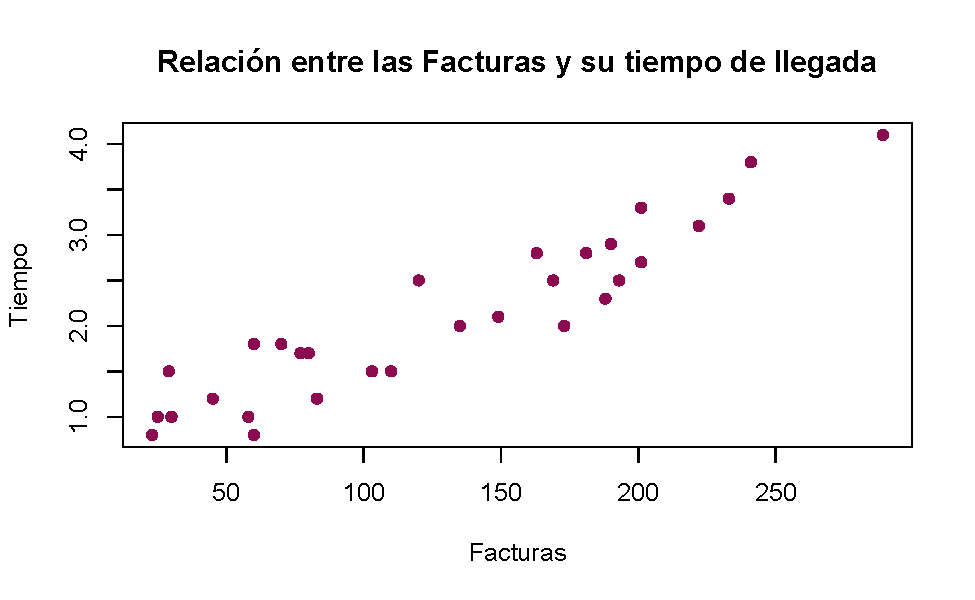
\includegraphics{_main_files/figure-latex/unnamed-chunk-6-1} \end{center}

Como podemos observar el gráfico nos grita que exite una posible relación lineal entre el número de facturas y el tiempo empleado para éstas.
Para confirmar nuestras sospechas vamos a calcular el coefieciente de correlación de Pearson:

\begin{Shaded}
\begin{Highlighting}[]
\FunctionTok{cor}\NormalTok{(Tiempo,Facturas)}
\end{Highlighting}
\end{Shaded}

\begin{verbatim}
[1] 0.9336877
\end{verbatim}

Es decir, r=0.9336 indica una fuerte relación lineal positiva entre el número de facturas procesadas y el tiempo. Entonces tiene ``sentido'' emplear un modelo de regresión lineal simple.

Ahora estimaremos los parámetros \(\beta_{0}\) y \(\beta_{1}\) con el método de mínimos cuadrados visto.

\begin{Shaded}
\begin{Highlighting}[]
\NormalTok{y}\OtherTok{=}\NormalTok{Dia}\SpecialCharTok{$}\NormalTok{Tiempo}
\NormalTok{x}\OtherTok{=}\NormalTok{Dia}\SpecialCharTok{$}\NormalTok{Facturas}
\NormalTok{y\_barra}\OtherTok{=}\FunctionTok{mean}\NormalTok{(y)}
\NormalTok{x\_barra}\OtherTok{=}\FunctionTok{mean}\NormalTok{(x) }
\NormalTok{Sxx}\OtherTok{=}\FunctionTok{sum}\NormalTok{((x}\SpecialCharTok{{-}}\NormalTok{x\_barra)}\SpecialCharTok{\^{}}\DecValTok{2}\NormalTok{) }
\NormalTok{Sxy}\OtherTok{=}\FunctionTok{sum}\NormalTok{((x}\SpecialCharTok{{-}}\NormalTok{x\_barra)}\SpecialCharTok{*}\NormalTok{(y}\SpecialCharTok{{-}}\NormalTok{y\_barra))}
\NormalTok{beta1}\OtherTok{=}\NormalTok{Sxy}\SpecialCharTok{/}\NormalTok{Sxx}
\NormalTok{beta0}\OtherTok{=}\NormalTok{y\_barra}\SpecialCharTok{{-}}\NormalTok{beta1}\SpecialCharTok{*}\NormalTok{x\_barra}
\end{Highlighting}
\end{Shaded}

Entonces \(\hat{\beta_{1}}\) será:

\begin{verbatim}
[1] 0.01129164
\end{verbatim}

y \(\hat{\beta_{0}}\) será:

\begin{verbatim}
[1] 0.6417099
\end{verbatim}

Ahora estimaremos el parámetro \(\beta\) con el método de mínimos cuadrados para un modelo sin intercepto.

\begin{Shaded}
\begin{Highlighting}[]
\NormalTok{beta\_gorro}\OtherTok{=}\FunctionTok{sum}\NormalTok{(x}\SpecialCharTok{*}\NormalTok{y)}\SpecialCharTok{/}\FunctionTok{sum}\NormalTok{(x}\SpecialCharTok{\^{}}\DecValTok{2}\NormalTok{)}
\end{Highlighting}
\end{Shaded}

Entonces \(\hat{\beta}\) será:

\begin{verbatim}
[1] 0.01503001
\end{verbatim}

\textbf{Residuales}

Ahora calcularemos los residuales, es decir la diferencia entre los valores observados y los valores estimados (\(e_i = y_i-\hat{y}_i\))

Primero calculamos el vector de los valores estimados \(\hat{y}\):

\begin{Shaded}
\begin{Highlighting}[]
\NormalTok{y\_gorro}\OtherTok{=}\NormalTok{beta0}\SpecialCharTok{+}\NormalTok{beta1}\SpecialCharTok{*}\NormalTok{x}
\end{Highlighting}
\end{Shaded}

Luego los residuales y los graficamos

\begin{Shaded}
\begin{Highlighting}[]
\NormalTok{e}\OtherTok{=}\NormalTok{y}\SpecialCharTok{{-}}\NormalTok{y\_gorro }
\FunctionTok{plot}\NormalTok{(e,}\AttributeTok{type =} \StringTok{"p"}\NormalTok{,}\AttributeTok{pch=}\DecValTok{16}\NormalTok{, }\AttributeTok{ylab=}\StringTok{"residuales"}\NormalTok{,}\AttributeTok{col=}\StringTok{"deeppink4"}\NormalTok{) }
\FunctionTok{abline}\NormalTok{(}\AttributeTok{a=}\DecValTok{0}\NormalTok{,}\AttributeTok{b=}\DecValTok{0}\NormalTok{, }\AttributeTok{col=}\StringTok{"green4"}\NormalTok{)}
\end{Highlighting}
\end{Shaded}

\begin{center}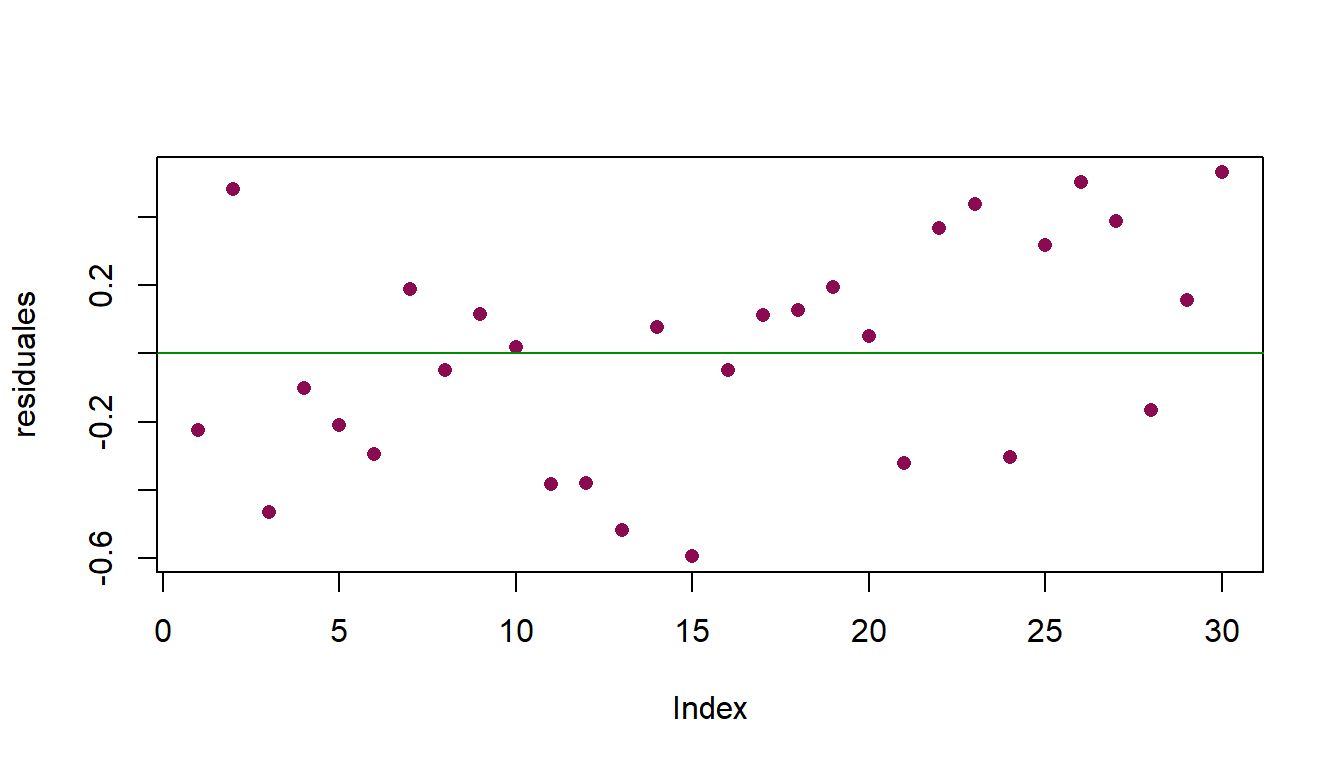
\includegraphics{_main_files/figure-latex/unnamed-chunk-14-1} \end{center}

Para que el modelo propuesto ajuste bien a los datos originales esperaríamos que los residuales estuvieran lo mas cercano al cero (linea amarilla). Mas adelante veremos como usar estos gráficos para verificar algunos de los supuestos del modelo.

\hypertarget{intervalos-de-confianza}{%
\chapter{Intervalos de confianza}\label{intervalos-de-confianza}}

Anteriormente hemos obtenido, de manera puntual, las estimaciones de los parámetros desconocidos del modelo de regresión lineal simple. Sin embargo, en ocasiones se puede tener una gran variabilidad en el ajuste de los parámetros, por lo que realizar inferencia puntual no siempre puede ser recomendable, es por ello que desarrollaremos intervalos de confianza para proporcionar estimaciones por intervalo en el cual, el parámetro de interés tenga una alta probabilidad de pertenecer a este conjunto.

\hypertarget{intervalo-para-beta_0}{%
\section{\texorpdfstring{Intervalo para \(\beta_{0}\)}{Intervalo para \textbackslash beta\_\{0\}}}\label{intervalo-para-beta_0}}

Dado que el estimador de \(\beta_{0}\) es una combinación lineal, de igual forma se tiene una combinación lineal de variables aleatorias normales independientes, por lo que \(\beta_{0}\) tiene una distribución normal asociada con media y varianza demostrada en el \textbf{teorema 2.4}.

\[\hat{\beta_{0}} \sim N \left( \beta_{0},\left(\frac{1}{n}+\frac{\overline{x}^2}{S_{xx}}\right)\sigma^2\right).\]
Estandarizando:

\[\frac{\hat{\beta_{0}}-\beta_{0}}{\sqrt{\left(\frac{1}{n}+\frac{\overline{x}^2}{S_{xx}}\right)\sigma^2}}\sim N (0,1).\]
Como \(\frac{(n-2)}{\sigma^2}\hat{\sigma}^2\sim\chi^2_{(n-2)}\) se tiene:

\[\frac{\frac{\hat{\beta_{0}}-\beta_{0}}{\sqrt{\left(\frac{1}{n}+\frac{\overline{x}^2}{S_{xx}}\right)\sigma^2}}}{\sqrt{\frac{\frac{(n-2)}{\sigma^2}\hat{\sigma}^2}{n-2}}}\sim t_{(n-2)}\]
Simplificando se obtiene la cantidad pivotal para \(\hat{\beta_{0}}:\)

\[\frac{\hat{\beta_{0}}-\beta_{0}}{\sqrt{\left(\frac{1}{n}+\frac{\overline{x}^2}{S_{xx}}\right)\hat{\sigma}^2}} \sim t_{(n-2)}\]
De esta manera, construyendo el intervalo de confianza con la cantidad pivotal:

\[\mathbf{P}\left[-t^{\alpha/2}_{(n-2)}<\frac{\hat{\beta_{0}}-\beta_{0}}{\sqrt{\left(\frac{1}{n}+\frac{\overline{x}^2}{S_{xx}}\right)\hat{\sigma}^2}}< t^{\alpha/2}_{(n-2)}\right]=1-\alpha\]
\[\mathbf{P}\left[-t^{\alpha/2}_{(n-2)}\sqrt{\left(\frac{1}{n}+\frac{\overline{x}^2}{S_{xx}}\right)\hat{\sigma}^2}<\hat{\beta_{0}}-\beta_{0}< t^{\alpha/2}_{(n-2)}\sqrt{\left(\frac{1}{n}+\frac{\overline{x}^2}{S_{xx}}\right)\hat{\sigma}^2}\right]=1-\alpha\]

\[\mathbf{P}\left[-t^{\alpha/2}_{(n-2)}\sqrt{\left(\frac{1}{n}+\frac{\overline{x}^2}{S_{xx}}\right)\hat{\sigma}^2}<\beta_{0}-\hat{\beta_{0}}< t^{\alpha/2}_{(n-2)}\sqrt{\left(\frac{1}{n}+\frac{\overline{x}^2}{S_{xx}}\right)\hat{\sigma}^2} \ \right]=1-\alpha\]
Sumando \(\hat{\beta_{0}}\) en todas las desigualdades:

\[\mathbf{P}\left[\hat{\beta_{0}}-t^{\alpha/2}_{(n-2)}\sqrt{\left(\frac{1}{n}+\frac{\overline{x}^2}{S_{xx}}\right)\hat{\sigma}^2}<\beta_{0}< \hat{\beta_{0}}+t^{\alpha/2}_{(n-2)}\sqrt{\left(\frac{1}{n}+\frac{\overline{x}^2}{S_{xx}}\right)\hat{\sigma}^2} \ \right]=1-\alpha\]
Por lo tanto, el intervalo de confianza \(1-\alpha\) para \(\beta_{0}\) es:

\[\beta_{0} \in \left( \hat{\beta_{0}}-t^{\alpha/2}_{(n-2)}\sqrt{\left(\frac{1}{n}+\frac{\overline{x}^2}{S_{xx}}\right)\hat{\sigma}^2} \ \ , \ \ \hat{\beta_{0}}+t^{\alpha/2}_{(n-2)}\sqrt{\left(\frac{1}{n}+\frac{\overline{x}^2}{S_{xx}}\right)\hat{\sigma}^2} \  \right).\]

\hypertarget{intervalo-para-beta_1}{%
\section{\texorpdfstring{Intervalo para \(\beta_{1}\)}{Intervalo para \textbackslash beta\_\{1\}}}\label{intervalo-para-beta_1}}

Dado que el estimador de \(\beta_{1}\) es una combinación lineal, de igual forma se tiene una combinación lineal de variables aleatorias normales independientes, por lo que \(\beta_{1}\) tiene una distribución normal asociada con media y varianza demostrada en el \textbf{teorema 2.4}.

\[\hat{\beta_{1}}\sim N \left(\beta_{1},\frac{\sigma^2}{S_{xx}}\right)\]
Estandarizando:

\[\frac{\hat{\beta_{1}}-\beta_{1}}{\sqrt{\frac{\sigma^2}{S_{xx}}}}\sim N(0,1).\]
Como \(\frac{(n-2)}{\sigma^2}\hat{\sigma}^2\sim\chi^2_{(n-2)}\) se tiene:

\[\frac{\frac{\hat{\beta_{1}}-\beta_{1}}{\sqrt{\frac{\sigma^2}{S_{xx}}}}}{\sqrt{\frac{\frac{(n-2)}{\sigma^2}\hat{\sigma}^2}{n-2}}} \sim t_{(n-2)}\]

Por lo tanto, simplificando se obtiene una cantidad pivotal para \(\hat{\beta_{1}}:\)

\[\frac{\hat{\beta_{1}}-\beta_{1}}{\sqrt{\frac{\hat{\sigma}^2}{S_{xx}}}}\sim t_{(n-2)}\]
Construyendo un intervalo de confianza \(1-\alpha\) para \(\beta_{1}\) se tiene que:

\[\mathbf{P}\left[-t^{\alpha/2}_{(n-2)} < \frac{\hat{\beta_{1}}-\beta_{1}}{\sqrt{\frac{\hat{\sigma}^2}{S_{xx}}}} < t^{\alpha/2}_{(n-2)}\right]=1-\alpha\]
\[\mathbf{P}\left[-t^{\alpha/2}_{(n-2)} \sqrt{\frac{\hat{\sigma}^2}{S_{xx}}} < \hat{\beta_{1}}-\beta_{1}< t^{\alpha/2}_{(n-2)} \sqrt{\frac{\hat{\sigma}^2}{S_{xx}}} \ \right]=1-\alpha\]

\[\mathbf{P}\left[-t^{\alpha/2}_{(n-2)} \sqrt{\frac{\hat{\sigma}^2}{S_{xx}}} < \beta_{1}-\hat{\beta_{1}}< t^{\alpha/2}_{(n-2)} \sqrt{\frac{\hat{\sigma}^2}{S_{xx}}} \ \right]=1-\alpha\]

Sumando \(\hat{\beta_{1}}\) en todas las desigualdades:

\[\mathbf{P}\left[\hat{\beta_{1}}-t^{\alpha/2}_{(n-2)} \sqrt{\frac{1}{S_{xx}}\hat{\sigma}^2} < \beta_{1}< \hat{\beta_{1}}+t^{\alpha/2}_{(n-2)} \sqrt{\frac{1}{S_{xx}}\hat{\sigma}^2} \ \right]=1-\alpha\]

Por lo tanto, el intervalo de confianza \(1-\alpha\) para \(\beta_{1}\) es:

\[\beta_{1} \in \left( \hat{\beta_{1}}-t^{\alpha/2}_{(n-2)} \sqrt{\frac{1}{S_{xx}}\hat{\sigma}^2} \ \ , \ \ \hat{\beta_{1}}+t^{\alpha/2}_{(n-2)} \sqrt{\frac{1}{S_{xx}}\hat{\sigma}^2} \  \right).\]

\hypertarget{intervalo-para-sigma2}{%
\section{\texorpdfstring{Intervalo para \(\sigma^2\)}{Intervalo para \textbackslash sigma\^{}2}}\label{intervalo-para-sigma2}}

Para construir el intervalo de confianza para \(\sigma^2\) se observa que se posee una cantidad pivotal asociada de la forma:

\[\frac{(n-2)\hat{\sigma}^2_{MC}}{\sigma^2}\sim \chi^2_{(n-2)}.\]
La distribución \(\chi^2\) no es una distribución simétrica por lo que se plantean los cuantiles \(W_{\alpha/2}\) y \(W_{1-\alpha/2}\) que corresponden a la valuación de la \(\chi^2_{(n-2)}\) en el cuantil \(\alpha/2\) y \(1-\alpha/2,\) respectivamente.

\[\mathbf{P}\left[W_{\alpha/2}<\frac{(n-2)\hat{\sigma}^2_{MC}}{\sigma^2}< W_{1-\alpha/2}\right]=1-\alpha\]

Obteniendo el recíproco en ambas partes de las desigualdades se observa que:

\[\mathbf{P}\left[\frac{1}{W_{\alpha/2}}>\frac{\sigma^2}{(n-2)\hat{\sigma}^2_{MC}}>\frac{1} {W_{1-\alpha/2}}\right]=1-\alpha\]
Reordenando el intervalo de confianza se tiene que:

\[\mathbf{P}\left[\frac{(n-2)\hat{\sigma}^2_{MC}}{W_{\alpha/2}}>\sigma^2>\frac{(n-2)\hat{\sigma}^2_{MC}} {W_{1-\alpha/2}}\right]=1-\alpha\]
Por la estimación insesgada propuesta para \(\sigma^2\) se sabe que \(\hat{\sigma}^2_{MC}=\frac{1}{n-2}\sum_{i=1}^{n}(y_i-\hat{y_{i}})^2\) así:

\[\mathbf{P}\left[\frac{\sum_{i=1}^{n}(y_i-\hat{y_{i}})^2}{W_{1-\alpha/2}}<\sigma^2<\frac{\sum_{i=1}^{n}(y_i-\hat{y_{i}})^2} {W_{\alpha/2}}\right]=1-\alpha\]

Por convención se usa que \(W_{1-\alpha/2}=\chi^{2(1-\alpha/2)}_{(n-2)}\) y \(W_{\alpha/2}=\chi^{2(\alpha/2)}_{(n-2)}.\) De esta manera el intervalo de confianza para \(\sigma^2\) es:

\[\mathbf{P}\left[\frac{\sum_{i=1}^{n}(y_i-\hat{y_{i}})^2}{\chi^{2(1-\alpha/2)}_{(n-2)}}<\sigma^2<\frac{\sum_{i=1}^{n}(y_i-\hat{y_{i}})^2} {\chi^{2(\alpha/2)}_{(n-2)}}\right]=1-\alpha,\]
reescribiendo el intervalo de confianza en su forma explícita:

\[\sigma^2 \in \left( \frac{\sum_{i=1}^{n}(y_i-\hat{y_{i}})^2}{\chi^{2(1-\alpha/2)}_{(n-2)}} \ \ , \ \ \frac{\sum_{i=1}^{n}(y_i-\hat{y_{i}})^2} {\chi^{2(\alpha/2)}_{(n-2)}} \right).\]

\hypertarget{intervalo-para-el-valor-esperado-y}{%
\section{\texorpdfstring{Intervalo para el valor esperado \(y\)}{Intervalo para el valor esperado y}}\label{intervalo-para-el-valor-esperado-y}}

Después de haber realizado un modelo de regresión lineal; como vimos en el teorema 2.1, el valor esperado de \(y_{i}\) es \(\mathbf{E}[y_{i}]=\beta_{0}+\beta_{1}x_{i},\) para toda \(i=1,\ldots,n,\) en el caso de que se conozca un nuevo valor \(x'\) de la variable regresora \(x\) entonces se podrá calcular el valor esperado de \(y\) al sustituir los estimadores de \(\beta_{0}\) y \(\beta_{1},\) respectivamente. Sin embargo, al realizar estas sustituciones se tiene asociada diversas variabilidades, como la desviación estándar de los estimadores. Es por ello que se realizan intervalos de confianza para el valor esperado \(y\) con la finalidad de aportar mejores ajustes con un nivel de significancia \(\alpha.\)

El valor esperado de \(y\) dado que se conoce un nuevo valor \(x'\) de \(x,\) hace referencia a la esperanza condicional de la forma \(\mathbf{E}[y|x=x']=\beta_{0}+\beta_{1}x',\) la cual es denotada como \(\mu_{x}=\mathbf{E}[y|x=x' ],\) sin embargo, al desconocer el valor de \(\beta_{0},\beta_{1}\) se realiza la estimación del valor de \(y\) usando los estimadores de mínimos cuadrados, es decir, \(\mathbf{E}[\widehat{y|x=x'}]=\hat{\beta_{0}}+\hat{\beta_{1}}x',\) usualmente escrita como \(\hat{\mu}_{x}=\mathbf{E}[\widehat{y|x=x'}].\)

Por ejemplo, suponga que después de estimar un modelo de regresión lineal simple se obtuvo como parámetros \(\hat{\beta_{0}}=3\) y \(\hat{\beta_{1}}=5,\) un año después se observa que el valor de la variable regresora es \(x'=10,\) de esta manera el valor esperado dado \(x'\) es:

\[\hat{\mu}_{x}=\hat{\beta_{0}}+\hat{\beta_{1}}x'.\]

Sustituyendo los valores del ejemplo:

\[\hat{\mu}_{x}=3+5(10)\]

\[\therefore \hat{\mu}_{x}=53.\]

Es decir, el valor esperado de \(y\) dado \(x'=10\) es 53 unidades. Debido a que cada \(y_{i}\) es una combinación lineal se sabe que los valores esperados se distribuyen con normalidad es decir:

\[\hat{\mu}_{x}\sim N \ (\mathbf{E}[\mu_{x}],Var[\mu_{x}]).\]

\textbf{Teorema 2.11} Sea \(\hat{\mu}_{x}=\hat{\beta_{0}}+\hat{\beta_{1}}x'\) el valor esperado de \(y\) dado \(x'\left( \mathbf{E}[\widehat{y|x=x'}]\right),\) entonces cumple con las propiedades de esperanza y varianza:

\textbf{a)} \(\mathbf{E}[\hat{\mu}_{x}]=\mu_{x}\) donde \(\mu_{x}=\beta_{0}+\beta_{1}x'.\)

\textbf{b)} \(Var[\hat{\mu}_{x}]=\left(\frac{1}{n}+\frac{(x'-\overline{x})^2}{S_{xx}}\right)\sigma^2.\)

\textbf{Demostración}

\textbf{a)} Para la esperanza se sabe que \(\hat{\mu}_{x}=\mathbf{E}[\widehat{y|x=x'}]\) así sustituyendo se sabe:

\[\mathbf{E}[\hat{\mu}_{x}]=\mathbf{E}\left[\hat{\beta_{0}}+\hat{\beta_{1}}x' \right].\]
Por propiedades de la esperanza se tiene:

\[\mathbf{E}[\hat{\mu}_{x}]=\mathbf{E}\left[\hat{\beta_{0}}\right]+x'\mathbf{E}\left[\hat{\beta_{1}} \right].\]
Por el \textbf{teorema 2.4} sabemos que los estimadores son insesgados:

\[\mathbf{E}[\hat{\mu}_{x}]=\beta_{0}+\beta_{1}x'\]
\[\therefore \mathbf{E}[\hat{\mu}_{x}]=\mu_{x}. \blacksquare\]
Por lo que es insesgado para \(\mu_{x},\) es decir, \(\mathbf{E}\left[\mathbf{E}[\widehat{y|x=x'}] \right]=\mathbf{E}[y|x=x'].\)

\textbf{b)} Para la varianza se tiene:

\[Var[\hat{\mu}_{x}]=Var\left[\hat{\beta_{0}}+\hat{\beta_{1}}x'\right]\]
\[Var[\hat{\mu}_{x}]=Var[\hat{\beta_{0}}]+Var[\hat{\beta_{1}}x']+2Cov(\hat{\beta_{0}},\hat{\beta_{1}}x').\]

Por el \textbf{teorema 2.5} se sabe que las varianzas de los estimadores son:

\[Var[\hat{\mu}_{x}]=\left( \frac{1}{n}+\frac{\overline{x}^2}{S_{xx}}\right)\sigma^2+x'^2Var[\hat{\beta_{1}}]+2x'Cov(\hat{\beta_{0}},\hat{\beta_{1}})\]

\[Var[\hat{\mu}_{x}]=\left( \frac{1}{n}+\frac{\overline{x}^2}{S_{xx}}\right)\sigma^2+\frac{x'^2}{S_{xx}}\sigma^2-2x'\frac{\overline{x}\sigma^2}{S_{xx}}\]
\[Var[\hat{\mu}_{x}]=\sigma^2\left( \frac{1}{n}+\frac{\overline{x}^2}{S_{xx}}+\frac{x'^2}{S_{xx}}-2x'\frac{\overline{x}}{S_{xx}}\right)\]
\[Var[\hat{\mu}_{x}]=\sigma^2\left( \frac{1}{n}+\frac{(x'-\overline{x})^2}{S_{xx}}\right). \blacksquare\]
De esta manera se busca construir un intervalo de confianza para el valor esperado de \(y\) dado \(x'(\mu_{x})\), y sabemos que el valor esperado se comporta de la forma:

\[\hat{\mu}_{x}\sim N\left(\mu_{x},\sigma^2\left( \frac{1}{n}+\frac{(x'-\overline{x})^2}{S_{xx}}\right)\right).\]
Estandarizando \(\hat{\mu}_{x}\) para obtener una normal estándar:

\[\frac{\hat{\mu}_{x}-\mu_{x}}{\sqrt{\sigma^2\left( \frac{1}{n}+\frac{(x'-\overline{x})^2}{S_{xx}}\right)}}\sim N(0,1)\]
Como \(\frac{(n-2)}{\sigma^2}\hat{\sigma}^2\sim\chi^2_{(n-2)}\) se tiene que el cociente entre una normal y una Ji-Cuadrada se distribuye como \(t\) de Student:

\[\frac{\frac{\hat{\mu}_{x}-\mu_{x}}{\sqrt{\sigma^2\left( \frac{1}{n}+\frac{(x'-\overline{x})^2}{S_{xx}}\right)}}}{\sqrt{\frac{\frac{(n-2)}{\sigma^2}\hat{\sigma}^2}{n-2}}}\sim t_{(n-2)}\]
Simplificando términos se tiene:

\[\frac{\hat{\mu}_{x}-\mu_{x}}{\sqrt{\hat{\sigma}^2\left( \frac{1}{n}+\frac{(x'-\overline{x})^2}{S_{xx}}\right)}}\sim t_{(n-2)}\]
Denotando a \(\hat{\sigma}_{x}^2=\hat{\sigma}^2\left(\frac{1}{n}+\frac{(x'-\overline{x})^2}{S_{xx}}\right)\) se tiene la cantidad pivotal para el valor esperado de \(y\) dado \(x\)

\[\frac{\hat{\mu}_{x}-\mu_{x}}{\sqrt{\hat{\sigma}_{x}^2}}\sim t_{(n-2)}.\]
Una vez hallado el estadístico a usar se construye el intervalo de confianza (\(1-\alpha\))x100 para \(\mu_{x}\).

\[\mathbf{P}\left[-t_{(n-2)}^{\alpha/2} < \frac{\hat{\mu}_{x}-\mu_{x}}{\sqrt{\hat{\sigma_{x}^2}}} < t_{(n-2)}^{\alpha/2}\right]=1-\alpha\]

\[\mathbf{P}\left[-t_{(n-2)}^{\alpha/2}\sqrt{\hat{\sigma_{x}^2}}<\hat{\mu}_{x}-\mu_{x}<t_{(n-2)}^{\alpha/2}\sqrt{\hat{\sigma_{x}^2}} \ \right]=1-\alpha\]
\[\mathbf{P}\left[-t_{(n-2)}^{\alpha/2}\sqrt{\hat{\sigma_{x}^2}}<\mu_{x}-\hat{\mu}_{x}<t_{(n-2)}^{\alpha/2}\sqrt{\hat{\sigma_{x}^2}} \ \right]=1-\alpha\]
\[\mathbf{P}\left[\hat{\mu}_{x}-t_{(n-2)}^{\alpha/2}\sqrt{\hat{\sigma_{x}^2}}<\mu_{x}<\hat{\mu}_{x}+t_{(n-2)}^{\alpha/2}\sqrt{\hat{\sigma_{x}^2}} \ \right]=1-\alpha\]
\[\therefore \mathbf{P}\left[\hat{\mu}_{x}-t_{(n-2)}^{\alpha/2}\sqrt{\left( \frac{1}{n}+\frac{(x'-\overline{x})^2}{S_{xx}}\right)\hat{\sigma}^2}<\mu_{x}<\hat{\mu}_{x}+t_{(n-2)}^{\alpha/2}\sqrt{\left( \frac{1}{n}+\frac{(x'-\overline{x})^2}{S_{xx}}\right)\hat{\sigma}^2} \ \ \right]=1-\alpha,\]
En su forma más compacta:

\[\mu_{x} \in \left(\hat{\mu}_{x}-t_{(n-2)}^{\alpha/2}\sqrt{\hat{\sigma_{x}^2}} \ \ , \ \ \hat{\mu}_{x}+t_{(n-2)}^{\alpha/2}\sqrt{\hat{\sigma_{x}^2}} \ \right).\]

entonces el intervalo de confianza para el valor esperado de \(y\) dado \(x'\) es:

\[\beta_{0}+\beta_{1}x' \in \left(\hat{\beta_{0}}+\hat{\beta_{1}}x'-t_{(n-2)}^{\alpha/2}\sqrt{\left( \frac{1}{n}+\frac{(x'-\overline{x})^2}{S_{xx}}\right)\hat{\sigma}^2} \ \ , \ \ \hat{\beta_{0}}+\hat{\beta_{1}}x'+t_{(n-2)}^{\alpha/2}\sqrt{\left( \frac{1}{n}+\frac{(x'-\overline{x})^2}{S_{xx}}\right)\hat{\sigma}^2} \ \right).\]

\hypertarget{intervalo-de-predicciuxf3n}{%
\section{Intervalo de predicción}\label{intervalo-de-predicciuxf3n}}

La diferencia significativa entre intervalos de predicción e intervalos de confianza para el valor esperado \(y,\) es que en el intervalo del valor esperado lo que se busca encontrar es el valor que en promedio se debería obtener \(y\) dado que se tiene una observación \(x\), es decir, la observación que cae sobre la recta de regresión de la forma \(\hat{y}=\hat{\beta_{0}}+\hat{\beta_{1}}x_{i},\) mientras que en un intervalo de predicción se ``predice'' valores futuros de \(y\) dado que se conoce o se estima un valor \(x,\) denotado como \(x^*,\) es decir, \(y=\beta_{0}+\beta_{1}x+\epsilon,\) por ende la predicción de valores de \(y\) es \(\hat{y_{x}}=\hat{\beta_{0}}+\hat{\beta_{1}}x^*+\epsilon\).

La varianza del valor de predicción que se debe considerar será la varianza del valor esperado \(\hat{\mu}_{x}\) pero además se añade la varianza del modelo de regresión lineal simple, es decir:

\[Var(\hat{y_{x}})=Var(\hat{\mu}_x)+Var(y).\]

El cual por el \textbf{teorema 2.1} y \textbf{teorema 2.11} tenemos:

\[Var(\hat{y_{x}})=\left( 1+ \frac{1}{n}+\frac{(x^*-\overline{x})^2}{S_{xx}} \ \right)\sigma^2.\]

\textbf{Teorema 2.12} La predicción de un valor de \(y\) dado que se conoce un valor \(x^*\) de la variable regresora \(x\) está dado por \(\hat{y_{x}}=\hat{\beta_{0}}+\hat{\beta_{1}}x^*+\epsilon,\) donde \(\epsilon\) satisface que \(\epsilon\sim N(0,\sigma^2)\) e independientemente a \(\beta_{0},\beta_{1},\) así la predicción cumple con las siguientes propiedades:

\textbf{a)} \(\mathbf{E}\left[\hat{y_{x}}\right]=\beta_{0}+\beta_{1}x^*.\)

\textbf{b)} \(Var\left[\hat{y_{x}}\right]=\left(1+ \frac{1}{n}+\frac{(x^*-\overline{x})^2}{S_{xx}}\right)\sigma^2.\)

\textbf{Demostración}

\textbf{a)} La esperanza de \(\hat{y_{x}}\) está dada por:

\[\mathbf{E}\left[\hat{y_{x}}\right]=\mathbf {E}\left[\hat{\beta_{0}}+\hat{\beta_{1}}x^*+ \epsilon\right]\]
Por linealidad de la esperanza

\[=\mathbf{E}\left[\hat{\beta_{0}}\right]+\mathbf{E}\left[\hat{\beta_{1}}x^*\right]+ \mathbf{E}\left[\epsilon\right]\]
Por el \textbf{teorema 2.4} e hipótesis

\[=\beta_{0}+\beta_{1}x^*+0\]

\[\therefore \mathbf{E}\left[\hat{y_{x}}\right]=\beta_{0}+\beta_{1}x^*. \ \blacksquare\]

\textbf{b)} La varianza de \(\hat{y_{x}}\) está dada por:

\[Var\left[\hat{y_{x}}\right]=Var\left[\hat{\beta_{0}}+\hat{\beta_{1}}x^*+\epsilon\right]\]
\[=Var\left[\hat{\beta_{0}}+\hat{\beta_{1}}x^*\right]+Var\left[\epsilon\right]+2Cov(\hat{\beta_{0}}+\hat{\beta_{1}}x^*,\epsilon)\]
Por independencia
\[=Var\left[\hat{\beta_{0}}+\hat{\beta_{1}}x^*\right]+Var\left[\epsilon\right]+2(0)\]
Por el \textbf{teorema 2.11} e hipótesis

\[=\left(\frac{1}{n}+\frac{(x^*-\overline{x})^2}{S_{xx}}\right)\sigma^2+\sigma^2\]

\[\therefore Var\left[\hat{y_{x}}\right]=\left(1+ \frac{1}{n}+\frac{(x^*-\overline{x})^2}{S_{xx}}\right)\sigma^2. \blacksquare\]

Usando los resultados, la estimación de valores futuros de \(y\) se comporta:

\[\hat{y_{x}} \sim N \left(y_{x},\sigma^2\left(1+ \frac{1}{n}+\frac{(x^*-\overline{x})^2}{S_{xx}} \ \right)\right),\]

donde \(y_{x}=\beta_{0}+\beta_{1}x^*.\) Estandarizando \(\hat{y_{x}}:\)

\[\frac{\hat{y_{x}}-y_{x}}{\sqrt{\sigma^2\left(1+ \frac{1}{n}+\frac{(x^*-\overline{x})^2}{S_{xx}}\right)}}\sim N (0,1)\]

Como \(\frac{(n-2)}{\sigma^2}\hat{\sigma}^2 \sim \chi^2_{(n-2)}\):

\[\frac{\frac{\hat{y_{x}}-y_{x}}{\sqrt{\sigma^2\left(1+ \frac{1}{n}+\frac{(x^*-\overline{x})^2}{S_{xx}}\right)}}}{\sqrt{\frac{\hat{\sigma}^2}{\sigma^2}}}\sim t_{(n-2)}.\]

Simplificando términos se tiene:

\[\frac{\hat{y_{x}}-y_{x}}{\sqrt{\hat{\sigma}^2\left(1+ \frac{1}{n}+\frac{(x^*-\overline{x})^2}{S_{xx}}\right)}}\sim t_{(n-2)}\]
Denotando a \(\sigma^2_{x}=\hat{\sigma}^2\left(1+ \frac{1}{n}+\frac{(x^*-\overline{x})^2}{S_{xx}}\right)\) se tiene la cantidad pivotal para el valor de \(y\) dado \(x\)

\[\frac{\hat{y_{x}}-y_{x}}{\sqrt{\sigma_{x}^2}}\sim t_{(n-2)}.\]

Por lo que construyendo el intervalo de predicción:

\[\mathbf{P}\left[-t^{\alpha/2}_{(n-2)}<\frac{\hat{y_{x}}-y_{x}}{\sqrt{\hat{\sigma}^2\left(1+ \frac{1}{n}+\frac{(x^*-\overline{x})^2}{S_{xx}}\right)}}<t^{\alpha/2}_{(n-2)}\right]=1-\alpha\]

\[\mathbf{P}\left[-t^{\alpha/2}_{(n-2)}\sqrt{\hat{\sigma}^2\left(1+ \frac{1}{n}+\frac{(x^*-\overline{x})^2}{S_{xx}}\right)}<\hat{y_{x}}-y_{x}<t^{\alpha/2}_{(n-2)}\sqrt{\hat{\sigma}^2\left(1+ \frac{1}{n}+\frac{(x^*-\overline{x})^2}{S_{xx}}\right)} \ \right]=1-\alpha\]

\[\mathbf{P}\left[-t^{\alpha/2}_{(n-2)}\sqrt{\hat{\sigma}^2\left(1+ \frac{1}{n}+\frac{(x^*-\overline{x})^2}{S_{xx}}\right)}<y_{x}-\hat{y_{x}}<t^{\alpha/2}_{(n-2)}\sqrt{\hat{\sigma}^2\left(1+ \frac{1}{n}+\frac{(x^*-\overline{x})^2}{S_{xx}}\right)} \ \right]=1-\alpha\]

\[\mathbf{P}\left[-t^{\alpha/2}_{(n-2)}\sqrt{\hat{\sigma}^2\left(1+ \frac{1}{n}+\frac{(x^*-\overline{x})^2}{S_{xx}}\right)}<\beta_{0}+\beta_{1}x^*-\hat{\beta_{0}}-\hat{\beta_{1}}x^*-\epsilon<t^{\alpha/2}_{(n-2)}\sqrt{\hat{\sigma}^2\left(1+ \frac{1}{n}+\frac{(x^*-\overline{x})^2}{S_{xx}}\right)} \ \right]=1-\alpha\]

\[\mathbf{P}\left[\hat{\beta_{0}}+\hat{\beta_{1}}x^*-t^{\alpha/2}_{(n-2)}\sqrt{\hat{\sigma}^2\left(1+ \frac{1}{n}+\frac{(x^*-\overline{x})^2}{S_{xx}}\right)}<\beta_{0}+\beta_{1}x^*-\epsilon<\hat{\beta_{0}}+\hat{\beta_{1}}x^*+t^{\alpha/2}_{(n-2)}\sqrt{\hat{\sigma}^2\left(1+ \frac{1}{n}+\frac{(x^*-\overline{x})^2}{S_{xx}}\right)} \ \right]=1-\alpha\]

Dado que \(\epsilon\) es una variable aleatoria simétrica y con media 0 se tiene:

\[\beta_{0}+\beta_{1}x^*+\epsilon \in \left[\hat{\beta_{0}}+\hat{\beta_{1}}x^*-t^{\alpha/2}_{(n-2)}\sqrt{\left(1+ \frac{1}{n}+\frac{(x^*-\overline{x})^2}{S_{xx}}\right)\hat{\sigma}^2},\hat{\beta_{0}}+\hat{\beta_{1}}x^*+t^{\alpha/2}_{(n-2)}\sqrt{\left(1+ \frac{1}{n}+\frac{(x^*-\overline{x})^2}{S_{xx}}\right)\hat{\sigma}^2} \ \right].\]

\hypertarget{ejemplo}{%
\subsection{Ejemplo}\label{ejemplo}}

Retomando los datos de la sección anterior, recordemos que el gerente del departamento de ventas de la compañía \textbf{CALLCENT} desea predecir, de alguna manera, el tiempo promedio que tardarían en procesar un número dado de facturas. Esto con el objetivo de llevar a cabo una buena logística de diversas operaciones dentro de la empresa.

Se ha recolectado, durante un periodo de 30 días, la información sobre el número de facturas procesadas (en nuestrio caso definimos como nuestra variable \(x\)) y el tiempo que tardan las mismas (que hemos definido como nuestra variable \(y\)).

Como se mencionó en la teoría para considerar la variabilidad en el ajuste provocada por el uso de una muestra aleatoria, además de estimación puntual, hay que realizar estimación por intervalos.

\textbf{Intervalos de confianza para \(\beta_{0}\) y \(\beta_{1}\)}

Entonces haremos el cálculo de los intervalos al \(95\%\) de confianza para ambos estimadores (\(\hat{\beta_{0}} \ , \ \hat{\beta_{1}}\)).

Como vimos en la sección anterior, debemos estimar \(\sigma^2\), recordemos que el estimador es: \[\hat{\sigma}^2=\frac{1}{n-2}\sum_{i=1}^{n}(y_{i}-\hat{y_{i}})^2\]

\begin{verbatim}
[1] 30
\end{verbatim}

\begin{Shaded}
\begin{Highlighting}[]
\NormalTok{s2\_gorro}\OtherTok{=}\DecValTok{1}\SpecialCharTok{/}\NormalTok{(n}\DecValTok{{-}2}\NormalTok{)}\SpecialCharTok{*}\FunctionTok{sum}\NormalTok{((y}\SpecialCharTok{{-}}\NormalTok{y\_gorro)}\SpecialCharTok{\^{}}\DecValTok{2}\NormalTok{)}
\NormalTok{s2\_gorro}
\end{Highlighting}
\end{Shaded}

\begin{verbatim}
[1] 0.1087505
\end{verbatim}

ya con \(\hat{\sigma}^2\) podemos construir los intervalos de confianza.

\begin{itemize}
\tightlist
\item
  Primero para \(\beta_{0}\), sustituyendo los valores en la siguiente ecuación:
\end{itemize}

\[\beta_{0} \in \left( \hat{\beta_{0}}-t^{\alpha/2}_{(n-2)}\sqrt{\left(\frac{1}{n}+\frac{\overline{x}^2}{S_{xx}}\right)\hat{\sigma}^2} \ \ , \ \ \hat{\beta_{0}}+t^{\alpha/2}_{(n-2)}\sqrt{\left(\frac{1}{n}+\frac{\overline{x}^2}{S_{xx}}\right)\hat{\sigma}^2} \ \right)\]

\begin{Shaded}
\begin{Highlighting}[]
\NormalTok{b0Liminf}\OtherTok{=}\NormalTok{beta0}\SpecialCharTok{{-}}\FunctionTok{qt}\NormalTok{(.}\DecValTok{975}\NormalTok{,n}\DecValTok{{-}2}\NormalTok{)}\SpecialCharTok{*}\FunctionTok{sqrt}\NormalTok{((}\DecValTok{1}\SpecialCharTok{/}\NormalTok{n}\SpecialCharTok{+}\NormalTok{x\_barra}\SpecialCharTok{\^{}}\DecValTok{2}\SpecialCharTok{/}\NormalTok{Sxx)}\SpecialCharTok{*}\NormalTok{s2\_gorro)}

\NormalTok{b0Limsup}\OtherTok{=}\NormalTok{beta0}\SpecialCharTok{+}\FunctionTok{qt}\NormalTok{(.}\DecValTok{975}\NormalTok{,n}\DecValTok{{-}2}\NormalTok{)}\SpecialCharTok{*}\FunctionTok{sqrt}\NormalTok{((}\DecValTok{1}\SpecialCharTok{/}\NormalTok{n}\SpecialCharTok{+}\NormalTok{x\_barra}\SpecialCharTok{\^{}}\DecValTok{2}\SpecialCharTok{/}\NormalTok{Sxx)}\SpecialCharTok{*}\NormalTok{s2\_gorro)}
\end{Highlighting}
\end{Shaded}

Entonces el intervalo del \(95\%\) de confianza para \(\beta_{0}\) es:

\begin{verbatim}
      b0Liminf  b0Limsup
[1,] 0.3912496 0.8921701
\end{verbatim}

\begin{itemize}
\tightlist
\item
  Ahora para \(\beta_1\), sustituyendo los valores en la siguiente ecuación:
\end{itemize}

\[\beta_{1} \in \left( \hat{\beta_{1}}-t^{\alpha/2}_{(n-2)} \sqrt{\frac{1}{S_{xx}}\hat{\sigma}^2} \ \ , \ \ \hat{\beta_{1}}+t^{\alpha/2}_{(n-2)} \sqrt{\frac{1}{S_{xx}}\hat{\sigma}^2} \ \right).\]

\begin{Shaded}
\begin{Highlighting}[]
\NormalTok{b1Liminf}\OtherTok{=}\NormalTok{beta1}\SpecialCharTok{{-}}\FunctionTok{qt}\NormalTok{(.}\DecValTok{975}\NormalTok{,n}\DecValTok{{-}2}\NormalTok{)}\SpecialCharTok{*}\FunctionTok{sqrt}\NormalTok{((}\DecValTok{1}\SpecialCharTok{/}\NormalTok{Sxx)}\SpecialCharTok{*}\NormalTok{s2\_gorro) }
\NormalTok{b1Limsup}\OtherTok{=}\NormalTok{beta1}\SpecialCharTok{+}\FunctionTok{qt}\NormalTok{(.}\DecValTok{975}\NormalTok{,n}\DecValTok{{-}2}\NormalTok{)}\SpecialCharTok{*}\FunctionTok{sqrt}\NormalTok{((}\DecValTok{1}\SpecialCharTok{/}\NormalTok{Sxx)}\SpecialCharTok{*}\NormalTok{s2\_gorro) }
\end{Highlighting}
\end{Shaded}

Entonces el intervalo del \(95\%\) de confianza para \(\beta_{1}\) es:

\begin{verbatim}
        b1Liminf   b1Limsup
[1,] 0.009615224 0.01296806
\end{verbatim}

\begin{itemize}
\tightlist
\item
  Y por último calculamos el intervalo de confianza para \(\sigma^2\), sustituyendo los valores en la siguiente ecuación:
\end{itemize}

\[\sigma^2 \in \left( \frac{\sum_{i=1}^{n}(y_i-\hat{y_{i}})^2}{\chi^{2(1-\alpha/2)}_{(n-2)}} \ \ , \ \ \frac{\sum_{i=1}^{n}(y_i-\hat{y_{i}})^2} {\chi^{2(\alpha/2)}_{(n-2)}} \right).\]

\begin{Shaded}
\begin{Highlighting}[]
\NormalTok{sigLiminf}\OtherTok{=}\FunctionTok{sum}\NormalTok{((y}\SpecialCharTok{{-}}\NormalTok{y\_gorro)}\SpecialCharTok{\^{}}\DecValTok{2}\NormalTok{)}\SpecialCharTok{/}\FunctionTok{qchisq}\NormalTok{(}\FloatTok{0.975}\NormalTok{,n}\DecValTok{{-}2}\NormalTok{) }
\NormalTok{sigLimsup}\OtherTok{=}\FunctionTok{sum}\NormalTok{((y}\SpecialCharTok{{-}}\NormalTok{y\_gorro)}\SpecialCharTok{\^{}}\DecValTok{2}\NormalTok{)}\SpecialCharTok{/}\FunctionTok{qchisq}\NormalTok{(}\FloatTok{0.025}\NormalTok{,n}\DecValTok{{-}2}\NormalTok{) }
\end{Highlighting}
\end{Shaded}

Entonces el intervalo del \(95\%\) de confianza para \(\beta_{1}\) es:

\begin{verbatim}
      sigLiminf sigLimsup
[1,] 0.06848759 0.1989182
\end{verbatim}

\textbf{Valor Esperado}

Ahora calcularemos el tiempo en horas promedio esperado para la fabulosa cantidad de 155 facturas.

\begin{Shaded}
\begin{Highlighting}[]
\NormalTok{x\_fac}\OtherTok{=}\DecValTok{155}
\NormalTok{y\_esperado}\OtherTok{=}\NormalTok{beta0}\SpecialCharTok{+}\NormalTok{beta1}\SpecialCharTok{*}\NormalTok{x\_fac}
\end{Highlighting}
\end{Shaded}

Entonces el tiempo en horas promedio esperado será:

\begin{verbatim}
[1] 2.391915
\end{verbatim}

Gráficamente se ve así:

\begin{center}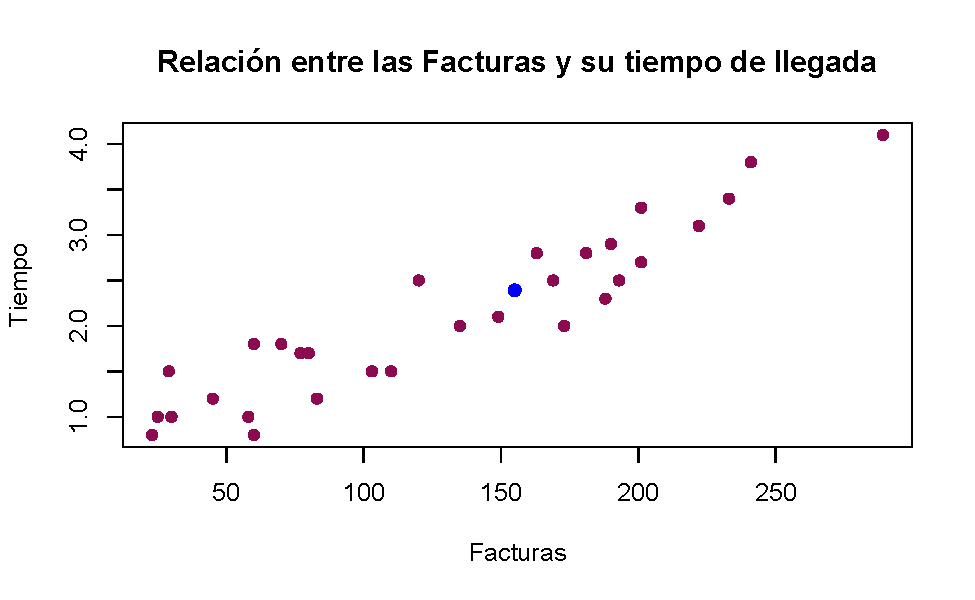
\includegraphics{_main_files/figure-latex/unnamed-chunk-25-1} \end{center}

Donde el punto azul es nuestro valor esperado.

\begin{itemize}
\tightlist
\item
  Y ahora construiremos su correspondiente intervalo del 99\% de confianza, sustituyendo en la siguiente ecuación:
\end{itemize}

\[\beta_{0}+\beta_{1}x' \in \left(\hat{\beta_{0}}+\hat{\beta_{1}}x'-t_{(n-2)}^{\alpha/2}\sqrt{\left( \frac{1}{n}+\frac{(x'-\overline{x})^2}{S_{xx}}\right)}\hat{\sigma}^2 \ \ , \ \ \hat{\beta_{0}}+\hat{\beta_{1}}x'+t_{(n-2)}^{\alpha/2}\sqrt{\left( \frac{1}{n}+\frac{(x'-\overline{x})^2}{S_{xx}}\right)\hat{\sigma}^2} \ \right).\]

\begin{Shaded}
\begin{Highlighting}[]
\NormalTok{y\_espLiminf}\OtherTok{=}\NormalTok{beta0}\SpecialCharTok{+}\NormalTok{beta1}\SpecialCharTok{*}\NormalTok{x\_fac}\SpecialCharTok{{-}}\FunctionTok{qt}\NormalTok{(.}\DecValTok{995}\NormalTok{,n}\DecValTok{{-}2}\NormalTok{)}\SpecialCharTok{*}\FunctionTok{sqrt}\NormalTok{((}\DecValTok{1}\SpecialCharTok{/}\NormalTok{n}\SpecialCharTok{+}\NormalTok{(x\_fac}\SpecialCharTok{{-}}\NormalTok{x\_barra)}\SpecialCharTok{\^{}}\DecValTok{2}\SpecialCharTok{/}\NormalTok{Sxx)}\SpecialCharTok{*}\NormalTok{s2\_gorro)}

\NormalTok{y\_espLimisup}\OtherTok{=}\NormalTok{beta0}\SpecialCharTok{+}\NormalTok{beta1}\SpecialCharTok{*}\NormalTok{x\_fac}\SpecialCharTok{+}\FunctionTok{qt}\NormalTok{(.}\DecValTok{995}\NormalTok{,n}\DecValTok{{-}2}\NormalTok{)}\SpecialCharTok{*}\FunctionTok{sqrt}\NormalTok{((}\DecValTok{1}\SpecialCharTok{/}\NormalTok{n}\SpecialCharTok{+}\NormalTok{(x\_fac}\SpecialCharTok{{-}}\NormalTok{x\_barra)}\SpecialCharTok{\^{}}\DecValTok{2}\SpecialCharTok{/}\NormalTok{Sxx)}\SpecialCharTok{*}\NormalTok{s2\_gorro)}
\end{Highlighting}
\end{Shaded}

Entonces el intervalo del \(99\%\) de confianza para el valor esperado de \(y\) es:

\begin{Shaded}
\begin{Highlighting}[]
\NormalTok{intery\_esperado}\OtherTok{=}\FunctionTok{cbind}\NormalTok{(y\_espLiminf,y\_espLimisup) }
\NormalTok{intery\_esperado}
\end{Highlighting}
\end{Shaded}

\begin{verbatim}
     y_espLiminf y_espLimisup
[1,]    2.216224     2.567605
\end{verbatim}

\begin{itemize}
\tightlist
\item
  El procedimiento es análogo al del valor esperado se aplica para el cálculo del intervalo de confianza para la predicción
\end{itemize}

\hypertarget{pruebas-de-hipuxf3tesis}{%
\chapter{Pruebas de hipótesis}\label{pruebas-de-hipuxf3tesis}}

El objetivo de la pruebas de hipótesis es poder escoger, a través de métodos estadísticos, la hipótesis capaz de retratar de mejor manera la realidad que se observa en la muestra.

\textbf{Definición 2.5} Una prueba de hipótesis es una regla de decisión que, cuando se ha obtenido los valores de la muestra observada, lleva a una decisión de aceptar o rechazar la hipótesis nula bajo una cierta consideración.

La hipótesis nula, la sentencia que se pone a prueba es denotada como \(H_0\), la hipótesis alternativa, el complemento de la hipótesis nula, es denotada como \(H_a.\)

En el modelo de regresión lineal simple, se desea realizar dos pruebas de hipótesis de gran importancia.

\begin{itemize}
\item
  \(\textbf{H}_0: \hat{\beta_{1}}=0 \ vs. \  \textbf{H}_a:\hat{\beta_{1}} \neq 0\)
\item
  \(\textbf{H}_0: \hat{\beta_{0}}=0 \ vs. \  \textbf{H}_a:\hat{\beta_{0}} \neq 0\)
\end{itemize}

Estas pruebas son de gran importancia, ya que la primera de ellas es probar si \(\beta_{1}\) es igual a cero, es decir, que el modelo no tenga pendiente y sea constante a través del tiempo, con un gran nivel de significancia dado. Si la prueba se rechaza entonces establece que el valor esperado de \(y\) depende de \(x\).

La segunda prueba de hipótesis analiza la posibilidad de que \(\beta_{0}=0\), si la prueba es aceptada implica que el modelo de regresión simple se comporta sin intercepto. Mientras que si se rechaza la hipótesis nula entonces \(\beta_{0}\neq 0,\) por lo cual el mejor ajuste para la muestra es un modelo de regresión simple con intercepto.

\hypertarget{pruebas-para-beta_0}{%
\section{\texorpdfstring{Pruebas para \(\beta_{0}\)}{Pruebas para \textbackslash beta\_\{0\}}}\label{pruebas-para-beta_0}}

Como se observó, la cantidad pivotal para \(\beta_{0}\) está determinado por \(t^{\alpha/2}_{(n-2)}\) con el estadístico:

\[t^*=\frac{\hat{\beta_{0}}-b_{0}}{\sqrt{\left(\frac{1}{n}+\frac{\overline{x}^2}{S_{xx}}\right)\hat{\sigma}^2}},\]

donde:

\[\hat{\sigma}^2=\frac{1}{n-2}\sum_{i=1}^{n}(y_{i}-\hat{y_{i}})^2.\]
Entonces las pruebas de hipótesis para \(\beta_{0},\) en sus tres casos, que el valor de \(\beta_{0}\) sea igual, inferior o superior al punto crítico deseado (\(b_{0}\)) tienen las siguientes reglas de decisión, con un nivel de significancia \(\alpha\).

\[
\begin{array}{|c|c|}
\hline
Hipótesis & Región\ de\ rechazo: \\
\hline
H_0:\beta_{0}=b_{0} \ vs. \ H_a:\beta_{0} \neq b_{0} & |t^*|>t^{\alpha/2}_{(n-2)} \\
\hline
H_0:\beta_{0}\leq b_{0} \ vs. \ H_a:\beta_{0} > b_{0} & t^*>t^{\alpha}_{(n-2)} \\
\hline
H_0:\beta_{0}\geq b_{0} \ vs. \ H_a:\beta_{0} < b_{0} & t^*<t^{1-\alpha}_{(n-2)} \\
\hline
\end{array}
\]

\textbf{Para ejemplificar}

Suponga que se quiere ajustar un modelo con intercepto o sin intercepto. En éste caso, conviene realizar una prueba de hipótesis de dos colas sobre \(\beta_{0}\) valuando el punto crítico \(b_{0}=0\), es decir, se desea probar que \(\beta_{0}=0\), ya que si, con un nivel de significancia \(\alpha\), se rechaza \(H_0\) se tiene evidencia de que el modelo a ajustar debería ser el modelo con intercepto. Detallando la prueba, en este caso en particular, tenemos:

\[\textbf{H}_0: \hat{\beta_{0}}=0 \ \ \ \ vs. \ \ \ \ \textbf{H}_a:\hat{\beta_{0}}\neq 0\]

La regla de decisión es rechazar \(H_0\) cuando el estadístico \(t^*=\frac{\hat{\beta_{0}}-b_{0}}{\sqrt{\left(\frac{1}{n}+\frac{\overline{x}^2}{S_{xx}}\right)\hat{\sigma}^2}}\) esté contenida en la región de rechazo. En este caso en particular, se tiene lo siguiente:

\[t^*=\frac{\hat{\beta_{0}}}{\sqrt{\left(\frac{1}{n}+\frac{\overline{x}^2}{S_{xx}}\right)\hat{\sigma}^2}}.\]

Por lo que se rechaza \(H_0\) cuando \(t^*<-t^{\alpha/2}_{(n-2)}\) o si \(t^*>t^{\alpha/2}_{(n-2)}\). Si se rechaza \(H_0\) entonces \(\beta_{0} \neq 0\) por lo que convendría realizar un modelo con intercepto; si no se rechaza la hipótesis nula con un nivel de significancia \(\alpha\), \(\beta_{0}=0,\) entonces el modelo sin intercepto sería el más óptimo para el conjunto de datos que se examina.

\hypertarget{prueba-para-beta_1}{%
\section{\texorpdfstring{Prueba para \(\beta_{1}\)}{Prueba para \textbackslash beta\_\{1\}}}\label{prueba-para-beta_1}}

Similar al caso anterior, \(\beta_{1}\) está determinado por \(t^{\alpha/2}_{(n-2)}\) con el estadístico:

\[t^*=\frac{\hat{\beta_{1}}-b_{1}}{\sqrt{\frac{\hat{\sigma}^2}{S_{xx}}}},\]

donde:

\[\hat{\sigma}^2=\frac{1}{n-2}\sum_{i=1}^{n}(y_{i}-\hat{y_{i}})^2.\]

Por lo tanto tenemos la prueba de hipótesis para \(\beta_{1}\) en sus tres casos, que el valor de \(\beta_{1}\) sea igual, inferior o superior al punto crítico deseado (\(b_{1}\)) y sus respectivas regiones de rechazo con un nivel de significancia \(\alpha.\)
\[
\begin{array}{|c|c|}
\hline
Hipótesis & Región\ de\ rechazo: \\
\hline
\hline
H_0:\beta_{1}=b_{1} \ vs. \ H_a:\beta_{1} \neq b_{1} & |t^*|>t^{\alpha/2}_{(n-2)} \\
\hline
H_0:\beta_{1}\leq b_{1} \ vs. \ H_a:\beta_{1} > b_{1} & t^*>t^{\alpha}_{(n-2)} \\
\hline
H_0:\beta_{1}\geq b_{1} \ vs. \ H_a:\beta_{1} < b_{1} & t^*<t^{1-\alpha}_{(n-2)} \\
\hline
\end{array}
\]

Para ejemplificar, suponga que quiere ajustar un modelo de regresión lineal simple, sin embargo, duda si realmente la variable respuesta \(y\) depende de la variable regresora \(x\), es decir, sospecha que \(\beta_{1}=0.\) Para ello se raliza la siguiente prueba de hipótesis valuando \(\beta_{1}\) en el punto crítico de interés \(b_{1}=0:\)

\[\textbf{H}_0: \hat{\beta_{1}}=0 \ \ \ \ vs. \ \ \ \ \textbf{H}_a:\hat{\beta_{1}} \neq 0\]

La regla de decisión es rechazar \(H_0\) cuando el estadístico \[t^*=\frac{\hat{\beta_{1}}}{\sqrt{\frac{\hat{\sigma}^2}{S_{xx}}}}\]

Esté contenida en la región de rechazo.Por lo que se rechaza \(H_0\) cuando \(t^*<-t^{\alpha/2}_{(n-2)}\) o si \(t^*>t^{\alpha/2}_{(n-2)}\).
Si se rechaza \(H_0\) entonces \(\beta_{1} \neq 0\) por lo que la variable respuesta \(y\) depende de la variable regresora \(x\); si no se rechaza \(H_0\) con un nivel de significancia \(\alpha\), \(\beta_{1}=0\), entonces la variable respuesta \(y\) no depende de la variable regresora \(x\), debido a ello un modelo de regresión no sería viable con esas variables.

\hypertarget{prueba-para-sigma2}{%
\section{\texorpdfstring{Prueba para \(\sigma^2\)}{Prueba para \textbackslash sigma\^{}2}}\label{prueba-para-sigma2}}

Para \(\sigma^2\) se tiene las siguientes reglas de decisión con un nivel de significancia \(\alpha:\)

\[
\begin{array}{|c|c|}
\hline
Hipótesis & Región\ de\ rechazo: \\
\hline
\hline
H_0:\sigma^2 = s \ vs. \ H_a:\sigma^2\neq s & t^*>\chi^{1-\alpha/2}_{(n-2)} \ \ ó \ \ t^*<\chi^{\alpha/2}_{(n-2)}  \\
\hline
H_0:\sigma^2 \leq s \ vs. \ H_a:\sigma^2 > s & t^*>\chi^{\alpha}_{(n-2)} \\
\hline
H_0:\sigma^2\geq s \ vs. \ H_a:\sigma^2 < s & t^*<\chi^{1-\alpha}_{(n-2)} \\
\hline
\end{array}
\]
donde el estadístico \(t^*:\)

\[t^*=\frac{(n-2)\hat{\sigma}^2}{s}\]
Con:
\[\hat{\sigma}^2=\frac{1}{n-2}\sum_{i=1}^{n}(y_{i}-\hat{y_{i}})^2.\]

\hypertarget{anuxe1lisis-de-la-varianza-anova}{%
\section{Análisis de la varianza (ANOVA)}\label{anuxe1lisis-de-la-varianza-anova}}

El análisis de la varianza, también llamado ANOVA por sus siglas en ingles (Analysis of Variance), mide la asociación lineal entre la variable respuesta \(y\) y la variable regresora \(x\).

La asociación lineal se logra cuando \(\beta_{1}\neq 0\), ya que en caso contrario, la estimación de \(y\) sería la media muestral \(\overline{y}\), y la variable regresora \(x\) no aportaría información. Entonces, al suponer \(\beta_{1}=0\), el ajuste de \(y\) estaría dado de la siguiente manera:

\[\hat{y}=\hat{\beta_{0}}+\hat{\beta_{1}}x_{i}.\]
Con \(\hat{\beta_{1}}=0:\)

\[\hat{y}=\hat{\beta_{0}}.\]

Por el \textbf{teorema 2.2} se sustituye la estimación de \(\hat{\beta_{0}}:\)

\[\hat{y}=\overline{y}-\overline{x}\hat{\beta_{1}}.\]

como \(\hat{\beta_{1}}=0:\)

\[\hat{y}=\overline{y}.\]
Es decir, no hay asociación lineal entre la variable respuesta \(y\) con la variable regresora \(x\). Es por ello que se desea demostrar que \(\beta_{1}\neq 0,\) mediante la siguiente prueba de hipótesis:

\[\textbf{H}_0:\hat{\beta_{1}}=0 \ \ \ vs. \ \ \ \textbf{H}_a:\hat{\beta_{1}} \neq 0\]
Se puede usar el estadístico de prueba de hipótesis para \(\beta_{1},\) con \(b1=0\). Y se tiene lo siguiente:

\[t^*=\frac{\hat{\beta_{1}}-b_{1}}{\sqrt{\frac{\hat{\sigma}^2}{S_{xx}}}} \sim t_{(n-2)}\]
De esta manera se rechaza la hipótesis nula y se supone que \(\beta_{1}\neq 0\) cuando \(|t^*|>t^{\alpha/2}_{(n-2)}\).

Sin embargo, en el análisis de la varianza, lo que se busca construir es otro estadístico que pueda ser usado cuando se tenga más de una variable explicativa. Es por ello que el matemático y biológo Ronald Fisher (1920), analizó la siguiente igualdad:

\[y_{i}-\overline{y}=(\hat{y_{i}}-\overline{y})+(y_{i}-\hat{y_{i}})\]

Lo que busca es fraccionar la distancia del valor observado respecto a la media, por la suma de la distancia del valor estimado a la media más la distancia del valor observado al valor estimado.

Obteniendo el cuadrado de la ecuación anterior:

\[(y_{i}-\overline{y})^2=(\hat{y_{i}}-\overline{y})^2+(y_{i}-\hat{y_{i}})^2+2(\hat{y_{i}}-\overline{y})(y_{i}-\hat{y_{i}})\]
Sumando sobre todos los valores:

\[\sum_{i=1}^{n}(y_{i}-\overline{y})^2=\sum_{i=1}^{n}(\hat{y_{i}}-\overline{y})^2+\sum_{i=1}^{n}(y_{i}-\hat{y_{i}})^2+2\sum_{i=1}^{n}(\hat{y_{i}}-\overline{y})(y_{i}-\hat{y_{i}})\]
Resolviendo la ecuación:

\[2\sum_{i=1}^{n}(\hat{y_{i}}-\overline{y})(y_{i}-\hat{y_{i}})=2\sum_{i=1}^{n}\hat{y_{i}}(y_{i}-\hat{y_{i}})-2\overline{y}\sum_{i=1}^{n}(y_{i}-\hat{y_{i}})^2.\]

Por la \textbf{definición 2.2}, se tiene \((y_{i}-\hat{y_{i}})=e_{i}\):

\[2\sum_{i=1}^{n}(\hat{y_{i}}-\overline{y})(y_{i}-\hat{y_{i}})=2\sum_{i=1}^{n}\hat{y_{i}}e_{i}-2\overline{y}\sum_{i=1}^{n}e_{i}.\]

Por el \textbf{teorema 2.3}, se sabe que \(\sum_{i=1}^{n}e_{i}=0\)

\[2\sum_{i=1}^{n}(\hat{y_{i}}-\overline{y})(y_{i}-\hat{y_{i}})=2\sum_{i=1}^{n}\hat{y_{i}}e_{i}\]
Por el \textbf{corolario 2}, \(\sum_{i=1}^{n}\hat{y_{i}}e_{i}=0\), por lo tanto tenemos:

\[\sum_{i=1}^{n}(y_{i}-\overline{y})^2=\sum_{i=1}^{n}(\hat{y_{i}}-\overline{y})^2+\sum_{i=1}^{n}(y_{i}-\hat{y_{i}})^2.\]

De esta manera se construye la \textbf{ANOVA}, generalmente se hace un cambio de notación:

\begin{itemize}
\item
  \(SC_{T}\) es la suma de cuadrados, mide la variabilidad de las observaciones del total corregido por la media y es denotado por \(SC_{T}=\sum_{i=1}^{n}(y_{i}-\overline{y})^2.\)
\item
  \(SC_{reg}\) es la suma de cuadrados de la regresión, mide la variabilidad de las observaciones \(y_{i}\) y la línea de regresión ajustada, es denotado por \(SC_{reg}=\sum_{i=1}^{n}(\hat{y_{i}}-\overline{y})^2.\)
\item
  \(SC_{error}\) es la suma de cuadrados del error, es decir mide la variación residual que queda sin explicar por la línea de regresión, es denotado por \(SC_{error}=\sum_{i=1}^{n}(y_{i}-\hat{y_{i}})^2.\)
\end{itemize}

De esta forma se tiene la siguiente igualdad:

\[SC_{T}=SC_{reg}+SC_{error}\]

Además se observa que:

\begin{itemize}
\item
  \(SC_{T}\) tiene \(n-1\) grados de libertad, ya que la suma \(\sum_{i=1}^{n}(y_{i}-\overline{y})^2\) es el núcleo de \((n-1)S^2=\frac{\sum_{i=1}^{n}(y_{i}-\overline{y})^2}{n-1}\) en el cual al estimar \(\mu\) con \(\overline{y}\) se pierde un grado de libertad.
\item
  \(SC_{reg}\) tiene 1 grado de libertad, ya que la regresión sólo tiene una variable indepediente \((x).\)
\item
  \(SC_{error}\) tiene \(n-2\) grados de libertad, ya que la regresión \(SC_{error}=SC_{T}-SC_{reg},\) en el cual se ha visto que \(SC_{T}\) y \(SC_{reg}\) tienen \(n-1\) y \(1\) grado de libertad, respectivamente, así los grados de libertad de \(SC_{error}=n-1-1,\) entonces \(SC_{error}\) tienen n-2 grados de libertad.
  Sabemos que el modelo de Regresión Lineal con errores normales tiene las siguientes propiedades:
\item
  \(\frac{SC_{reg}}{\sigma^2}\sim \chi^2_{(1)}.\)
\item
  \(\frac{(n-2)\hat{\sigma}^2}{\sigma^2}=\frac{SC_{error}}{\sigma^2}\sim\chi^2_{(n-2)}.\)
\item
  Además \(SC_{reg}\) es independiente a \(SC_{error}.\)
\end{itemize}

Debido a un resultado de probabilidad se sabe que si \(x \sim \chi^2_{(n)}\) y \(y \sim \chi^2_{(m)}\) y si \(x\) es independiente a \(y\) entonces:

\[\frac{x/n}{y/m}\sim F_{(n,m)}\]

De esta forma se puede aplicar la prueba \(F\) de Fisher en el análisis de varianza para probar las hipótesis. La prueba \(F\) consiste en dividir \(SC_{reg}\) entre sus grados de libertad y éste dividirlo entre \(SC_{error}\) que a su vez está dividida entre sus grados de libertad, de esta manera:

\[F=\frac{\frac{SC_{reg}}{1}}{\frac{SC_{error}}{n-2}}\]

Aplicando el resultado:

\[F=\frac{\frac{SC_{reg}}{1}}{\frac{SC_{error}}{n-2}} \sim F_{(1,n-2)}\]
Ahora se ocupará el \textbf{Cuadrado Medio} denotado como \textbf{CM}, la cual corresponde a la Suma de Cuadrados entre los grados de libertad. Así, se define al cuadrado medio de la regresión \(CM_{reg}\) y al cuadrado medio del error \(CM_{error}\) como:

\[
\begin{array}{c c c}
CM_{reg}=\frac{SC_{reg}}{1} & y & CM_{error}=\frac{SC_{error}}{n-2}. \\
\end{array}
\]

De igual manera, haciendo el ajuste, la prueba \(F\) queda definida como:

\[F=\frac{CM_{reg}}{CM_{error}}.\]
Observamos que \(SC_{reg}=\hat{\beta_{1}}S_{xy}\) entonces:

\[F=\frac{\hat{\beta_{1}}S_{xy}}{CM_{error}}.\]
De esta manera, la región de rechazo para la prueba de hipótesis \(H_0:\beta_{1}=0\) es:

\[\frac{\hat{\beta_{1}}S_{xy}}{CM_{error}}>(t^{\alpha/2}_{(n-2)})^2\]
La cual es equivalente a la prueba t.

\[\frac{|\hat{\beta_{1}}|}{\sqrt{Var(\hat{\beta_{1}})}} > t^{\alpha/2}_{(n-2)}.\]

Ya que si \(x \sim t_{(n-1)}\) entonces \(x^2 \sim F_{(1,n-2)}.\)

El siguiente cuadro resume la información anterior, mejor conocida como \textbf{Tabla ANOVA:}

\[
\begin{array}{|c| c| c| c| c|}
\hline
&Grados\ de\ libertad & Suma\ de\ Cuadrados & Cuadrado\ Medio & Prueba\ F \\
\hline
\hline
Regresión & 1   & \sum_{i=1}^{n}(\hat{y_{i}}-\overline{y})^2=\hat{\beta_{1}}S_{xy} & SC_{reg} & \frac{CM_{reg}}{CM_{error}} \\
\hline
Error     & n-2 & \sum_{i=1}^{n}(y_{i}-\hat{y_{i}})^2=SC_{T}-\hat{\beta_{1}}S_{xy} & \frac{SC_{error}}{n-2} & -\\
\hline 
Total     & n-1 & \sum_{i=1}^{n}(y_{i}-\overline{y})^2 & - & - \\
\hline
\end{array}
\]

\hypertarget{coeficiente-de-determinaciuxf3n}{%
\section{Coeficiente de determinación}\label{coeficiente-de-determinaciuxf3n}}

El coeficiente de determinación, con frecuencia se le asocia a la proporción de la variación explicada por el regresor \(x\), ya que \(0<SC_{reg}<SC_{T}\) entonces los valores del coeficiente de determinación están entre \(0<R^2<1.\)

Se define el coeficiente de determinación del modelo de regresión como:

\[R^2=\frac{SC_{reg}}{SC_{T}}=1-\frac{Sc_{error}}{SC_{T}}.\]

\hypertarget{propiedades-de-r2}{%
\section{\texorpdfstring{Propiedades de \(R^2\)}{Propiedades de R\^{}2}}\label{propiedades-de-r2}}

El coeficiente de determinación \(R^2\) satisface las siguientes propiedades:

\begin{itemize}
\item
  \(0 \leq R^2 \leq 1\) ya que \(0 \leq SC_{error} \leq SC_{T}.\)
\item
  Si \(R^2=1\) entonces tenemos que \(SC_{reg}=SC_{T}\) y \(\frac{SC_{error}}{SC_{T}}=0.\)
\item
  Si \(R^2=0\) entonces \(SC_{error}=SC_{T}.\)
\end{itemize}

En particular, se buscan valores de \(R^2\) cercanos a 1, ya que esto indica que la mayor parte de la variabilidad de \(y\) es determinada o explicada por el modelo de regresión. La magnitud de \(R^2\) también depende del rango de variabilidad de la variable regresora. En general \(R^2\) aumenta a medida que la propagación de los valores de \(x\) aumenta, y disminuye a medida que la propagación de los valores de \(x\) disminuyan, siempre que el modelo asumido es correcto.

\[
\begin{array}{|c |c|}
\hline
\textbf{Valor de} \ R^2 & \textbf{Tipo de correlación} \\
\hline
\hline
R^2=0 & No\ hay\ correlación \\
0<R^2<0.25 & Correlación\ muy\ débil \\
0.25\leq R^2 < 0.5 & Correlación\ débil \\
0.5 \leq R^2 < 0.75 & Correlación\ moderada \\
0.75 \leq R^2 < 0.9 & Correlación\ fuerte \\
0.9 \leq R^2 < 1 & Correlación\ muy\ fuerte \\
R^2=1 & Correlación\ perfecta \\
\hline
\end{array}
\]

\hypertarget{relaciuxf3n-r2-y-la-correlaciuxf3n-de-pearson}{%
\section{\texorpdfstring{Relación \(R^2\) y la correlación de Pearson}{Relación R\^{}2 y la correlación de Pearson}}\label{relaciuxf3n-r2-y-la-correlaciuxf3n-de-pearson}}

El coeficiente de correlación de Pearson entre \(x_{1},\ldots, x_{n}\) y \(y_{1},\ldots, y_{n}\) se define como:

\[r=\frac{S_{xy}}{\sqrt{S_{xx}S_{yy}}}.\]
\("r"\) toma valores de \(-1\) a \(1\), dónde si \(r\) toma el valor de \(1\) decimos que hay una relación lineal positiva, si \(r\) toma el valor de \(-1\) decimos que hay una relación lineal negativa y finalmente si toma el valor de \(0\) decimos que no hay una relación entre variables.

Para el modelo de regresión lineal, en particular, se cumple que:

\[r^2=R^2.\]

\hypertarget{ejemplo-1}{%
\subsection{Ejemplo}\label{ejemplo-1}}

En las secciones anteriores tomamos los datos de \textbf{CALLCENT} y comenzamos a resolver el problema que el gerente nos planteó de poder
predecir, de alguna manera, el tiempo promedio que tardarían en procesar un número dado de facturas.

Se ha recolectado, durante un periodo de 30 días, la información sobre el número de facturas procesadas (en nuestrio caso definimos como nuestra variable \(x\)) y el tiempo que tardan las mismas (que hemos definido como nuestra variable \(y\)).

Verificamos gráficamente que hubiera una relación lineal entre las variables, estimamos los parámetros del modelo de regresión lineal simple con intercepto y sin intercepto. Luego construimos intervalos de confianza para los parámetros estimados, para el valor esperado y la predicción.

Como se mencionó en nuestro capítulo debemos aplicar pruebas estadísticas que nos aseguren que las estimaciones de los parámetros serán distintos de cero.

\hypertarget{prueba-de-hipuxf3tesis-para-beta_0-y-beta_1}{%
\subsubsection*{\texorpdfstring{Prueba de hipótesis para \(\beta_{0}\) y \(\beta_{1}\)}{Prueba de hipótesis para \textbackslash beta\_\{0\} y \textbackslash beta\_\{1\}}}\label{prueba-de-hipuxf3tesis-para-beta_0-y-beta_1}}


Haremos el cálculo del estadístico de prueba para probar la hipótesis: \(\textbf{H}_0=\hat{\beta_{0}}=0 \ \ \ vs \ \ \ \textbf{H}_a \neq 0\) con una confianza del \(90\%\) y sustituimos en la siguiente ecuación:

\[t^*=\frac{\hat{\beta_{0}}}{\sqrt{\left(\frac{1}{n}+\frac{\overline{x}^2}{S_{xx}}\right)\hat{\sigma}^2}}.\]

\begin{Shaded}
\begin{Highlighting}[]
\NormalTok{t\_est}\OtherTok{=}\NormalTok{beta0}\SpecialCharTok{/}\FunctionTok{sqrt}\NormalTok{((}\DecValTok{1}\SpecialCharTok{/}\NormalTok{n}\SpecialCharTok{+}\NormalTok{x\_barra}\SpecialCharTok{\^{}}\DecValTok{2}\SpecialCharTok{/}\NormalTok{Sxx)}\SpecialCharTok{*}\NormalTok{s2\_gorro)}

\NormalTok{t\_est}
\end{Highlighting}
\end{Shaded}

\begin{verbatim}
[1] 5.24827
\end{verbatim}

Ahora buscamos el cuantil de la distribución \(t-Student\) para comprar nuestro estadístico.

\begin{Shaded}
\begin{Highlighting}[]
\NormalTok{qt}\OtherTok{=}\FunctionTok{qt}\NormalTok{(.}\DecValTok{95}\NormalTok{,n}\DecValTok{{-}2}\NormalTok{) }
\NormalTok{qt}
\end{Highlighting}
\end{Shaded}

\begin{verbatim}
[1] 1.701131
\end{verbatim}

Como nuestro estadístico (5.2482) es mayor que (1.7011). Entonces rechazamos \(\textbf{H}_0\). Por lo tanto con una confianza del \(90\%\) podemos decir que \(\beta_{0} \neq 0.\)

Ahora haremos la prueba para la hipótesis \(\textbf{H}_0:\hat{\beta_{1}}=0 \ \ vs \ \ \textbf{H}_{a}:\hat{\beta_{1}} \neq 0\) con una confianza del \(90\%\). Sustituimos en la siguiente ecuación:

\[t^*=\frac{\hat{\beta_{1}}}{\sqrt{\frac{\hat{\sigma}^2}{S_{xx}}}}\]

\begin{Shaded}
\begin{Highlighting}[]
\NormalTok{t\_est}\OtherTok{=}\NormalTok{beta1}\SpecialCharTok{/}\FunctionTok{sqrt}\NormalTok{(s2\_gorro}\SpecialCharTok{/}\NormalTok{Sxx)}

\NormalTok{t\_est}
\end{Highlighting}
\end{Shaded}

\begin{verbatim}
[1] 13.79718
\end{verbatim}

Ahora buscamos el cuantil de la distribución \(t-Student\) para comparar nuestro estadístico:

\begin{Shaded}
\begin{Highlighting}[]
\NormalTok{qt}\OtherTok{=}\FunctionTok{qt}\NormalTok{(.}\DecValTok{95}\NormalTok{,n}\DecValTok{{-}2}\NormalTok{) }

\NormalTok{qt}
\end{Highlighting}
\end{Shaded}

\begin{verbatim}
[1] 1.701131
\end{verbatim}

Como nuestro estadístico (13.7971) es mayor que (1.7011). Entonces rechazamos \(\textbf{H}_0\). Por lo tanto con una confianza del \(90\%\) podemos decir que \(\beta_{1} \neq 0.\)

Con éstas dos pruebas corroboramos que los datos ajustan a un modelo de regresión lineal que considera a la variable facturas y el intercepto, esto debido a que ambos parámetros resultaron ser distintos de cero.

\begin{itemize}
\item
  Si la prueba de hipótesis para \(\beta_{0 }\) hubiera resultado en no rechazar \(\textbf{H}_0\) entonces, se buscaría ajustar un modelo sin intercepto.
\item
  Si la prueba de hipótesis para \(\beta_{1}\) hubiera resultado en no rechazar \(\textbf{H}_0\) entonces, se buscaría ajustar un modelo con otra variable (diferente a las facturas) ya que los datos estarían diciendo que la variable facturas no es significativa para explicar el tiempo promedio de su llegada.
\end{itemize}

\hypertarget{coeficiente-de-determinaciuxf3n-1}{%
\subsubsection*{Coeficiente de determinación}\label{coeficiente-de-determinaciuxf3n-1}}


Por último vamos a calcular el coeficiente de determinación de nuestro modelo. Como se menciona en nuestro capítulo, este coeficiente mide la proporción de la variación explicada por el modelo en relación a la variación total existente en los datos, y por eso es un valor entre 0 y 1.

Y sustituiremos en la siguiente expresión:

\[R^2=\frac{\hat{\beta_{1}}S_{xy}}{\sum_{i=1}^{n}(y_{i}-\overline{y})^2}\]

\begin{Shaded}
\begin{Highlighting}[]
\NormalTok{R\_2}\OtherTok{=}\NormalTok{(beta1}\SpecialCharTok{*}\NormalTok{Sxy)}\SpecialCharTok{/}\FunctionTok{sum}\NormalTok{((y}\SpecialCharTok{{-}}\NormalTok{y\_barra)}\SpecialCharTok{\^{}}\DecValTok{2}\NormalTok{)}
\NormalTok{R\_2}
\end{Highlighting}
\end{Shaded}

\begin{verbatim}
[1] 0.8717727
\end{verbatim}

Lo que quiere decir que nuestro modelo está explicando \(87.17\%\) de la variabilidad observada en la variable facturas. El ideal es tener un modelo que explique el \(100\%\) pero como vimos, debido a que estamos ajustando una recta y esta no pasa por todos los puntos algún error en el ajuste estamos cometiendo.

\hypertarget{validaciuxf3n-de-supuestos}{%
\chapter{Validación de supuestos}\label{validaciuxf3n-de-supuestos}}

El modelo de regresión lineal es una buena herramienta de estimación, sin embargo, en dicho proceso se hace uso de diversos supuestos que deben cumplirse para que los resultados obtenidos sean acordes a la teoría desarrollada, que hasta el momento no se le había prestado gran atención. Estos supuestos los vimos en la \textbf{definición 2.1} para el caso de regresión lineal simple.
A manera de resumen y de forma general los supuestos que deben cumplirse son: la esperanza de los errores \(\epsilon\) tienen media cero, es decir, \(\mathbf{E}[\epsilon]=0\), varianza constante sobre los errores, es decir, \((Var(\epsilon)=\sigma^2)\), los errores no se encuentran correlacionados entre si, es decir, \((Cov(\epsilon_{i},\epsilon_{j})\forall i\neq j)\), por último, los errores tienen distribución normal con media cero y varianza \(\sigma^2\), es decir, \(\epsilon \sim \mathbf{N}(0,\sigma^2).\)

Es por ello que analizaremos y verificaremos el cumplimiento de los supuestos, la mayoría de estas validaciones se basan bajo el principio del análisis de residuales.

\hypertarget{anuxe1lisis-de-residuales}{%
\section{Análisis de residuales}\label{anuxe1lisis-de-residuales}}

Anteriormente definimos los residuales como \(e_{i}=y_{i}-\hat{y_{i}}\), el cual su nombre deriva de la obtención del residual o diferencia que existe entre la línea de regresión ajustada y los valores observados de la variable respuesta \(y_{i}\); esta cantidad residual es un buen ajuste debría ser cercana a cero, pues cuando esto sucede se tiene que \(y_{i} \approx \hat{y_{i}}\) debido a ello se opta por trabajar con los residuales para verificar el cumplimiento de los supuestos.

Muchas pruebas usan como base modificaciones o tipos específicos de residuos, es por esta razón que se indagará sobre los diversos tipos más conocidos.

\textbf{residuales ordinarios}

Los residuales ordinarios o simplemente residuales, miden la diferencia entre la línea de regresión y la variable respuesta \(y_{i}\), es por ello que se definen como:

\[e_{i}=y_{i}-\hat{y_{i}}  \ \ \ \ \ \ \ \ i=1,2,\ldots ,n.\]
La desventaja que presentan estos residuales, es que depende de cada \(y_{i}\) por lo que observaciones atípicas puede generar grandes residuales, ocasionando que pueda existir gran variabilidad al considerarse los errores en forma conjunta.

\textbf{residuales estandarizados}

Una forma de disminuir esta variabilidad consiste en dividir a los residuales \(e_{i}\) entre la varianza global, es decir:

\[d_{i}=\frac{e_{i}}{\sqrt{\sigma^2}}\]

Una propiedad importante es que si \(e_{i}\) sigue una distribución normal, entonces al dividirlo entre la desviación estándar, se tiene que los residuales estandarizados siguen una distribución normal estándar.

\textbf{residuales estudentizados}

Los residuales estudentizados se basan en la idea de involucrar la varianza de cada observación en el cálculo de los residuales, pues teóricamente los residuales no tiene varianza constante.

Como se demostrará en el corolario A (ver \(Apéndice\)), se sabe que \(e=(I-H)\underline{Y}\); en donde \(H=X(X'X)^{-1}X'\) la definimos como \textbf{matriz sombrero}.
De esta manera calculando la varianza de los errores se tiene:

\textbf{Corolario 6} Sea \(\underline{e}\) los residuales del modelo entonces la varianza de \(\underline{e}\) está dada por:

\[Var(\underline{e})=\sigma^2(I-H)\]

\textbf{Demostración:}

\[Var(\underline{e})=Var((I-H)\underline{Y})\]

\[Var(\underline{e})=(I-H)'Var(\underline{Y})(I-H)\]
Sabemos que \((I-H)\) es simétrica (ver \(apéndice\))

\[Var(\underline{e})=(I-H)(I-H)Var(\underline{Y})\]
Sabemos quue \((I-H)\) es idempotente (ver \(apéndice\))

\[Var(\underline{e})=(I-H)Var(\underline{Y})\]
Por el \textbf{teorema B} (demostrado en \(apéndice\))

\textbf{Teorema B} Sea una variable de interés \(\underline{Y}\), llamada \textbf{dependiente}, relacionada con dos o más variables explicativas\(x_{1},x_{2},\ldots,x_{k}\),
entonces:

\textbf{a)} \(\mathbf{E}[\underline{Y}]= \beta_{0}+\beta_{1}x_{1}+\beta_{2}x_{2}+ \ldots + \beta_{k}x_{k}.\)

\textbf{b)} \(Var(\underline{Y})= \sigma^2.\)

\[\therefore Var(\underline{e})=\sigma^2(I-H). \blacksquare\]

La varianza de cada residual no es constante para todas las observaciones es por ello que el resultado depende de la siguiente forma:

\[Var(e_{i})=\sigma^2(1-h_{ii})\]
donde \(h_{ii}\) correspondiente al \(i-ésimo\) elemento de la diagonal de la matriz sombrero \(H\).

Cada residual se divide entre su varianza obteniendo de esta forma lo que se conoce como \textbf{residuales estudentizados}, los cuales se definen como:

\[r_{i}=\frac{e_{i}}{\sqrt{\hat{\sigma}^2(1-h_{ii})}}\]
Debido a la construcción de los \textbf{residuales estudentizados} se logra estandarizar de mejor manera a los residuales del modelo. Si se cumple que cada residual \(e_{i}\) sigue una distribución normal entonces los residuales estudentizados siguen una distribución aproximada a una \(t-student\) con \(n-k-1\) grados de libertad.

\hypertarget{supuesto-de-normalidad}{%
\section{Supuesto de normalidad}\label{supuesto-de-normalidad}}

Como se mencionó, en el modelo de regresión lineal se tiene el supuesto de que los errores tienen distribución normal con media cero y varianza \(\sigma^2\). Debido a la construcción del modelo, este supuesto puede presentar desviaciones en la distribución, en la cual, serias desviaciones de ésta puede ocasionar que las estimaciones dadas sean erróneas, principalmente se pueden observar en la construcción de intervalos de confianza o pruebas de hipótesis, ya que las cantidades pivotales se basan en la premisa de normalidad en los errores, por lo que desviaciones significativas provocan una mala aproximación o cálculo; además que pruebas de hipótesis subsecuentes basadas en distribuciones como la \(t\) de Student o la \(F\) de Fisher presentan malas estadísticas para la toma de decisiones.

\hypertarget{validaciuxf3n-del-supuesto-de-normalidad}{%
\subsection{Validación del supuesto de normalidad}\label{validaciuxf3n-del-supuesto-de-normalidad}}

Para validar el supuesto de normalidad existen varios métodos, el primero de ellos es de forma visual, a través de las denominadas gráficas cuantil-cuantil, o también denominadas QQ-plot, ésta gráfica es muy usada para comprobar si una muestra sigue una determinada distribución. El procedimiento se basa en ordenar los residuales \((e_{i})\) en orden ascendente los cuales se mostrarán en el eje horizontal \(X\), mientras que el eje vertical \(Y\) se muestra al valor esperado de la estadística de orden de una distribución normal.
El valor esperado se denota como:

\[\mathbf{E}[e_{i}]=\phi^{-1}\left[\frac{i-\frac{1}{2}}{n}\right].\]

Donde la función \(\phi^{-1}\) es la distribución inversa de una normal. Si los resultados se comportaran de manera normal la gráfica de cuantiles de los errores pareciera que siguen una marcada línea de \(45^\circ\), por lo que valores fuera de la línea recta indicarían una distribución no normal.

\[\mbox{Diversas distribuciones en gráficas QQ-plot}\]

\begin{center}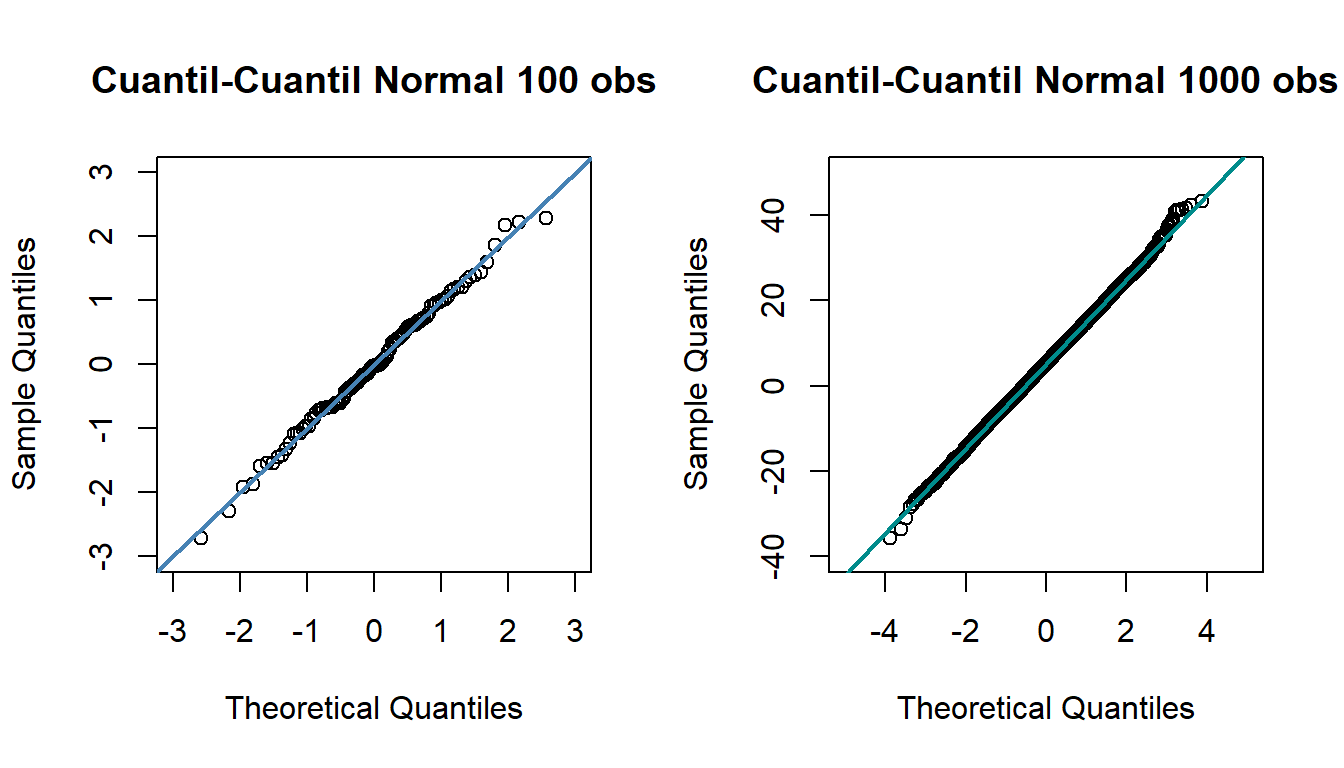
\includegraphics{_main_files/figure-latex/unnamed-chunk-33-1} \end{center}

\begin{center}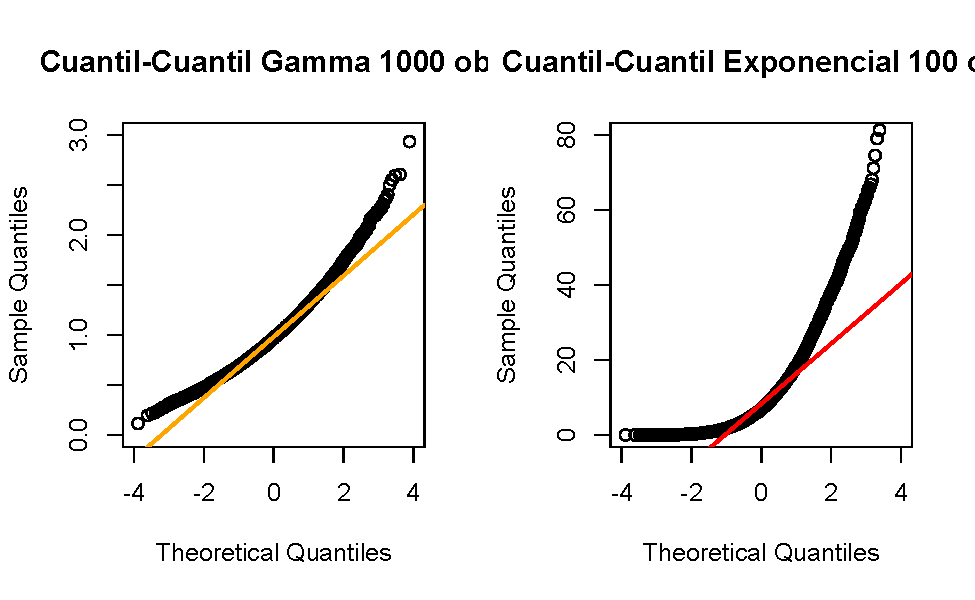
\includegraphics{_main_files/figure-latex/unnamed-chunk-34-1} \end{center}

Lo que podemos observar, es que las dos muestras superiores siguen una distribución normal, sin embargo, la primera tiene pocas observaciones por lo que algunos puntos se encuentran cercanos a la recta azul, línea que representa la distribución normal ideal, pero pocas veces la muestra toca esta línea y las colas presentan mucha variabilidad, la gráfica de la derecha al tener tamaño de muestra mayor, se aprecia que muchos datos caen sobre la recta, presentando ligeras irregularidades en la cola, tanto superior como inferior, por lo que se puede asumir, que las muestras siguen una distribución normal.

Por último, las gráficas inferiores, representan a una muestra con distribución gamma y exponencial, respectivamente, al no seguir una distribución normal, los datos salen completamente de la línea recta marcada, por lo que es evidente que no se comportan con normalidad.

Otro procedimiento para validar el supuesto de normalidad, es mediante pruebas de bondad de ajuste, sin embargo hay que tener cuidado, ya que los errores no son independientes entre si, debido a que están correlacionados, mientras que las pruebas de bondad de ajuste asumen precisamente que las observaciones son independientes entre si. Windfried Stute demostró que pruebas como la Anderson-Darling convergen a la distribución teórica aunque la independencia de los errores no se cumpla, debido a que se basan en el proceso empírico. Sin embargo, las pruebas deben de usarse como una medida de aproximación y no como regla de decisión.

\hypertarget{supuesto-de-linealidad}{%
\section{Supuesto de linealidad}\label{supuesto-de-linealidad}}

En la construcción del modelo de regresión lineal se asume que la relación entre \(X_{j}\) y \(Y\) es lineal, para cada \(j \in 1,\ldots,k\), con \(k\) el número de variables regresoras con el que fue ajustado el modelo.

Sin embargo, la anterior afirmación no siempre se cumple, es por ello que se valida este supuesto de manera gráfica. Debido a lo complejo que es una gráfica en más de tres dimensiones, se verá que en el modelo de regresión múltiple con \(k\) regresores se ajusta un hiperplano de dimensión \(k\).

Cuando \(k\geq 4\) se recomienda realizar gráficas individuales para comprobar la linealidad de la variable explicativa \(X_{j}\) y la variable del interés \(Y\).

Aunque este método proporciona una buena aproximación para saber si dos variables son lineales o no, este tipo de análisis puede proporcionar conclusiones erróneas cuando los coeficientes tienen magnitudes distintas ya que se analiza la relación marginal de la variable respuesta con cada variable explicativa. Es por ello que se opta trabajar mediante un análisis de residuales, en este análisis se grafican los errores estandarizados contra los valores observados de cada variable explicativa, en el cual el cumplimiento de la hipótesis daría como resultado ruido blanco con media 0 y varianza \(\sigma^2.\)

Cuando se detecte problemas de linealidad entre variables explicativas y la variable de interés, el ajuste del modelo es malo, debido a que la varianza presenta problemas en la estimación y por consecuencia estadísticas, se usa \(\sigma^2\) en su desarrollo lo cual hereda errores en sus cálculos.

\hypertarget{supuesto-de-homocedasticidad}{%
\section{Supuesto de homocedasticidad}\label{supuesto-de-homocedasticidad}}

Se dice que una muestra es homocedástica cuando la varianza es constante a lo largo de todas las observaciones, es decir, no varia conforme se presentan nuevas observaciones. Mientras una muestra heterocedástica se presenta cuando hay variaciones de la varianza conforme se presentan nuevas observaciones.

Las desviaciones en el supuesto de homocedasticidad pueden observarse mediante gráficas, la más óptima para el análisis es realizar una gráfica de dispersión en el que se muestre la relación entre los valores ajustados \(\underline{\hat{Y}}\) contra los residuales estandarizados \(d_{i}\). Si la varianza es constante entonces la gráfica fluctuará entre el eje horizontal de manera simétrica, asemejando a una distribución uniforme, y sin seguir algún tipo de patrón, ya que típicamente se considera que la mayor parte de los errores deben estar contenidos en franjas horizontales delimitados por el eje vertical entre \(y=-2\) y \(y=2\).

\[\mbox{Muestra homocedástica y una Muestra heterocedástica}\]

\begin{center}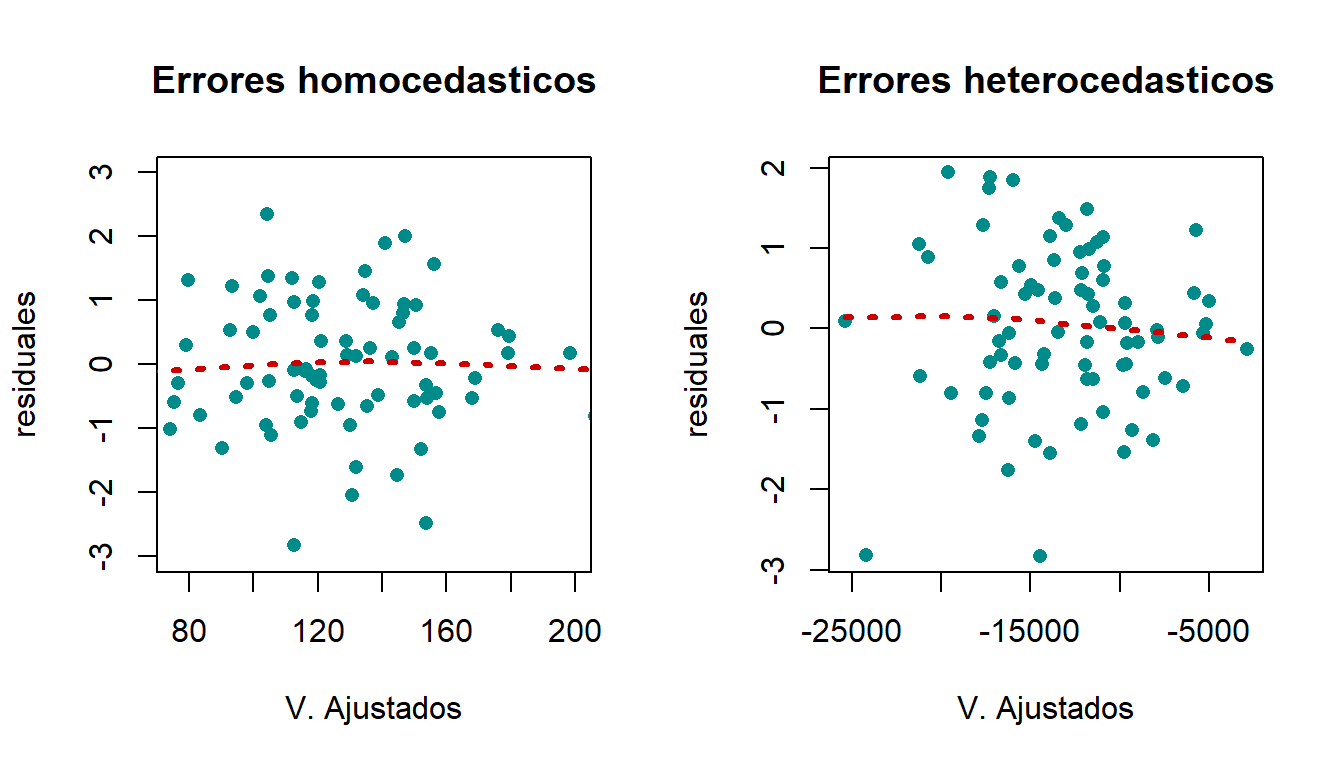
\includegraphics{_main_files/figure-latex/unnamed-chunk-35-1} \end{center}

\begin{center}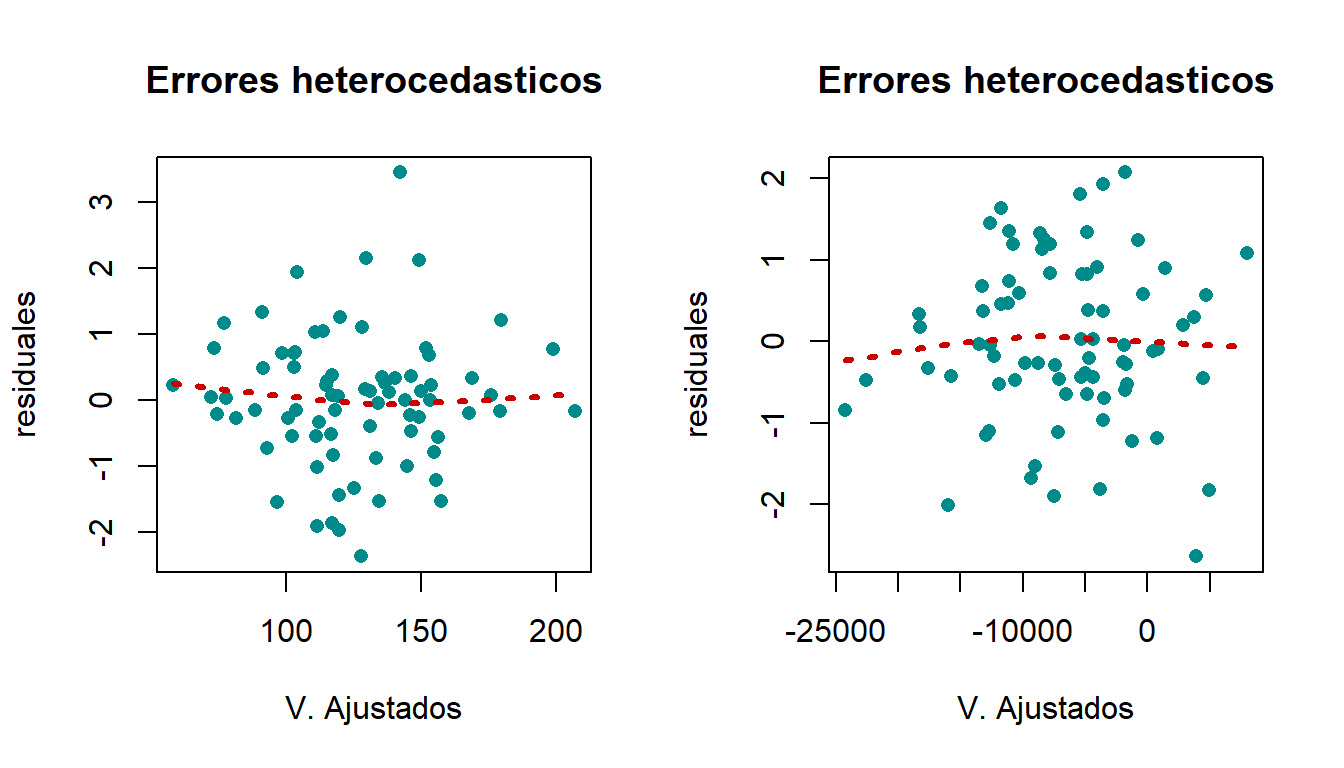
\includegraphics{_main_files/figure-latex/unnamed-chunk-35-2} \end{center}

Como estamos observando, la primera imagen corresponde a una muestra homocedástica pues los errores se distribuyen a lo largo del eje horizontal, además que éstos fluctúan entre \(y=-2\) y \(y=2\) distribuidos de una manera simétrica. Mientras que la segunda gráfica muestra que los errores fluctúan entre -2 y 2, sin embargo los resultados siguen un patrón de tender hacia a la media conforme se presentan nuevas observaciones, simulando un megáfono, por lo que se dice que la muestra sigue una tendencia heterocedástica.

Por último las gráficas ubicadas en la parte inferior, muestran como conforme se presentan nuevas observaciones los errores se alejan de la media, por lo que son muestras heterocedásticas.

Existen métodos más formales para probar homocedasticidad mediante pruebas de hipótesis, una de las que se desarrollarán a continuación.

\hypertarget{prueba-de-breusch-pagan}{%
\subsection{Prueba de Breusch-Pagan}\label{prueba-de-breusch-pagan}}

La prueba de Breusch-Pagan fue desarrollada en 1979 por los estadísticos Trevor Breusch y Adrian Pagan, se utiliza para determinar si una muestra presenta problemas de homocedasticidad o heterocedasticidad en un modelo de regresión lineal. El método consiste en analizar si la varianza estimada de los residuales de una regresión depende directamente de los valores obtenidos de las variables independientes, uno de los supuestos de esta prueba es que los errores deben comportarse con normalidad.

La prueba de Breusch-Pagan contrasta como hipótesis nula el cumplimiento de homocedasticidad, por lo que se tiene la siguiente prueba de hipótesis.

\[\textbf{H}_0: \ \mbox{Muestra homocedástica  i.e.} \ \ \ \sigma^2_{j}=\sigma^2 \ \ \ \ vs  \ \ \ \
\textbf{H}_a:  \ \mbox{Muestra Heterocedástica  i.e.} \ \ \ \sigma^2_{j} \neq \sigma^2 \ \ \ \ \forall  \ \ j = 1,\ldots,n.\]

El procedimiento se basa en calcular los residuales estandarizados al cuadrado \(\left( \tilde{e}^2_{j}=\frac{e^2_{j}}{\sigma^2}\right)\); Con ello se realiza una regresión lineal tomando como variable respuesta a cada \(\tilde{e}_{j}\) al cuadrado y con variables explicativas dentro del conjunto de variables exógenas Z:

\[\tilde{e}_{j}^{2}=\gamma_{0}+\gamma_{1}Z_{1}+ \ldots + \gamma_{n}Z_{n}\]

Después se procede a calcular la suma de cuadrados de la regresión del modelo con los errores estandarizados divididos entre 2, \(\frac{SC_{reg}}{2},\) donde \(SC_{reg}=\underline{Y}'(H-\frac{1}{n}J)\underline{Y}'\); Breusch-Pagan descubrieron que este estadístico sigue asintóticamente una distribución ji-cuadrada con \(k\) grados de libertad, siendo \(k\) el número de variables del modelo. Por lo que la región de rechazo para \(H_0\) sucede cuando la estadística \(\frac{SC_{reg}}{2}\) es mayor al cuantil de una ji-cuadrada con \(k\) grados de libertad con un nivel de significancia \(\alpha\), es decir:

\[\frac{SC_{reg}}{2}> \chi^{2(\alpha)}_{k}.\]
En otro caso no se tiene evidencia sificiente para rechazar la hipótesis nula.

En \(R\) la prueba de Breusch-Pagan puede ser fácilmente implementada, suponga que se tiene una muestra en el que se ha implementado el procedimiento de regresión lineal en \(R \ (lm(Y \sim X))\), por lo que aplicándo el siguiente código se tiene:

\begin{verbatim}

    studentized Breusch-Pagan test

data:  modelo1
BP = 0.026689, df = 1, p-value = 0.8702
\end{verbatim}

Se observa que en el anterior caso particular, la prueba supone como válida la hipótesis nula; la homocedasticidad de muestra debido a que el \(p-value\) es alto, (de 0.8702), lo que conlleva a que no se rechace la hipótesis nula con un nivel de significancia \(\alpha=0.05\), por lo que se acepta que la muestra se comporta con homocedasticidad.

\hypertarget{prueba-de-white}{%
\subsection{Prueba de White}\label{prueba-de-white}}

La prueba de White es similar a la prueba de Breusch-Pagan, sin embargo, se considera que ésta prueba es más general pues no requiere que los errores sigan una distribución normal.

La prueba de White fue propuesta por Hilbert White en 1980, como alternativa a la prueba de Breusch-Pagan, el procedimiento es similar, se analiza si la varianza estimada de los residuos de una regresión depende directamente de los valores obtenidos.

El test contrasta como hipótesis nula el cumplimiento de homocedasticidad, por lo que se tiene la siguiente prueba de hipótesis.

\[\textbf{H}_0: \  \mbox{Muestra homocedástica  i.e.}  \ \ \  \sigma^2_{j}=\sigma^2 \ \ \ \ vs  \ \ \ \
\textbf{H}_a: \  \mbox{Muestra Heterocedástica i.e.}  \ \ \  \sigma^2_{j} \neq \sigma^2  \ \ \ \ \forall  \ j = 1,\ldots,n.\]

El procedimiento se basa en calcular los residuales estandarizados al cuadrado \(\left( \tilde{e}^2_{j}=\frac{e^2_{j}}{\sigma^2}\right)\); Con ello se realiza una regresión lineal tomando como variable respuesta a cada \(\tilde{e}_{j}\) al cuadrado y el producto cruzado de variables explicativas dentro del conjunto de variables exógenas Z:

\[\tilde{e}_{j}^{2}=\gamma_{0}+\gamma_{1}Z_{1i}+ \ldots + \gamma_{k}Z_{ki}+\gamma_{k+1}Z^2_{1k}+\ldots + \gamma_{k+k}Z_{1k}Z_{ki}+\gamma{k+k+1}Z_{2k}Z_{1k}+\ldots + \gamma{tk}Z^2_{kk}+\epsilon\]
Del anterior ajuste de regresión se procede a calcular el coeficiente de determinación \(R^2=\frac{SC_{reg}}{SC_{T}}\) y sea n el tamaño de la muestra, entonces la estadística \(nR^2\) sigue asintóticamente una distribución ji-cuadrada con \(k\) grados de libertad, siendo \(k\) el número de variables del modelo original.Por lo que la región de rechazo para \(H_0\) sucede cuando la estadística \(nR^2\) es mayor al cuantil de una ji-cuadrada con \(k\) grados de libertad con un nivel de significancia \(\alpha\), es decir:

\[nR^2>\chi^{2(\alpha}_{k}).\]
En otro caso no se tiene evidencia suficiente para rechazar la hipótesis nula.

Se observa que en el anterior caso particular la prueba de White supone como válida la hipótesis nula la homocedasticidad de la muestra, debido a que el \(p-value\) es alto, (de 0.5244), lo que conlleva a que no se rechace la hipótesis nula con un nivel de significancia \(\alpha=0.05\), por lo que se acepta que la muestra se comporta con homocedasticidad.

\hypertarget{ejemplo-2}{%
\subsection{Ejemplo}\label{ejemplo-2}}

En las secciones anteriores tomamos los datos de \textbf{CALLCENT} y comenzamos a resolver el problema que el gerente nos planteó de poder
predecir, de alguna manera, el tiempo promedio que tardarían en procesar un número dado de facturas.

Se ha recolectado, durante un periodo de 30 días, la información sobre el número de facturas procesadas (en nuestrio caso definimos como nuestra variable \(x\)) y el tiempo que tardan las mismas (que hemos definido como nuestra variable \(y\)).

Verificamos gráficamente que hubiera una relación lineal entre las variables, estimamos los parámetros del modelo de regresión lineal simple con intercepto y sin intercepto. Luego construimos intervalos de confianza para los parámetros estimados, para el valor esperado y la predicción. Realizamos pruebas de hipótesis sobre los estimadores de los parámetros. Calculamos el coeficiente de determinación y realizamos un análisis de varianza sobre el modelo seleccionado.

Como se mencionó en nuestro capítulo debemos verificar que los supuestoshechos para ajustar este modelo de regresión lineal simple se cumplen.

Esta vez vamos a ocupar la función en R para el modelo de regresión que es \textbf{lm()}.

\begin{Shaded}
\begin{Highlighting}[]
\NormalTok{M1}\OtherTok{=}\FunctionTok{lm}\NormalTok{(Tiempo}\SpecialCharTok{\textasciitilde{}}\NormalTok{Facturas)}
\NormalTok{M1}
\end{Highlighting}
\end{Shaded}

\begin{verbatim}

Call:
lm(formula = Tiempo ~ Facturas)

Coefficients:
(Intercept)     Facturas  
    0.64171      0.01129  
\end{verbatim}

\textbf{Residuales}

Entonces primero calcularemos los diferentes residuales vistos. Se presentaran solamente los primeros 6 residuos de las 30 observaciones y un diagrama de dispersión.

\begin{itemize}
\tightlist
\item
  \(\textbf{Los residuales ordinarios}\)
\end{itemize}

\begin{Shaded}
\begin{Highlighting}[]
\FunctionTok{head}\NormalTok{(M1}\SpecialCharTok{$}\NormalTok{residuals)}
\end{Highlighting}
\end{Shaded}

\begin{verbatim}
         1          2          3          4          5          6 
-0.2241648  0.4807915 -0.4645390 -0.1014177 -0.2113303 -0.2966252 
\end{verbatim}

\begin{center}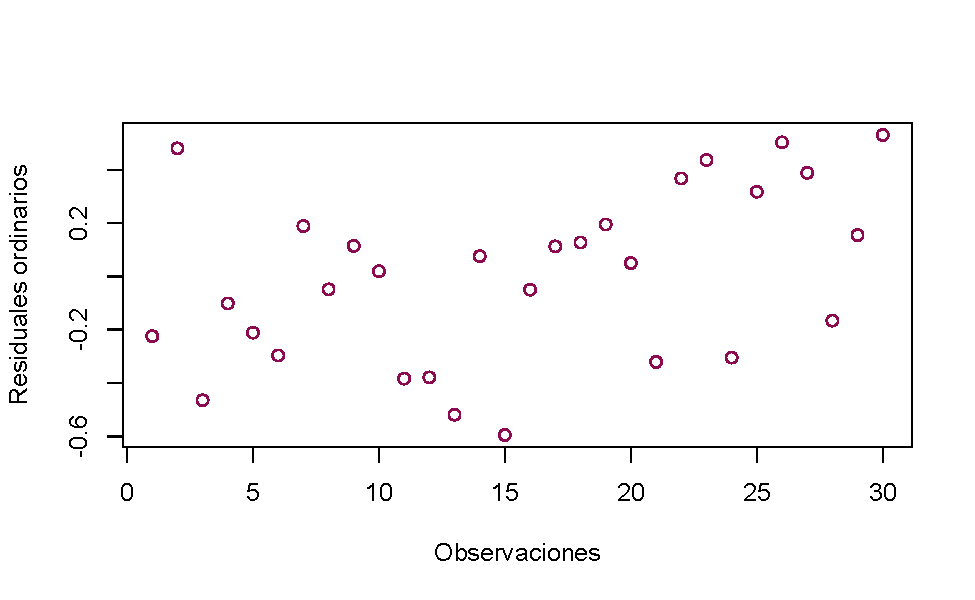
\includegraphics{_main_files/figure-latex/unnamed-chunk-41-1} \end{center}

\begin{itemize}
\tightlist
\item
  \(\textbf{Los residuales estandarizados}\)
\end{itemize}

\begin{Shaded}
\begin{Highlighting}[]
\FunctionTok{head}\NormalTok{(}\FunctionTok{rstandard}\NormalTok{(M1))}
\end{Highlighting}
\end{Shaded}

\begin{verbatim}
         1          2          3          4          5          6 
-0.6921686  1.5065958 -1.4483299 -0.3248760 -0.6625061 -0.9303669 
\end{verbatim}

\begin{Shaded}
\begin{Highlighting}[]
\FunctionTok{plot}\NormalTok{(}\FunctionTok{rstandard}\NormalTok{(M1),}\AttributeTok{col=}\StringTok{"deeppink4"}\NormalTok{,}\AttributeTok{ylab=}\StringTok{"Residuales estandarizados"}\NormalTok{, }\AttributeTok{xlab=}\StringTok{"Observaciones"}\NormalTok{)}
\end{Highlighting}
\end{Shaded}

\begin{center}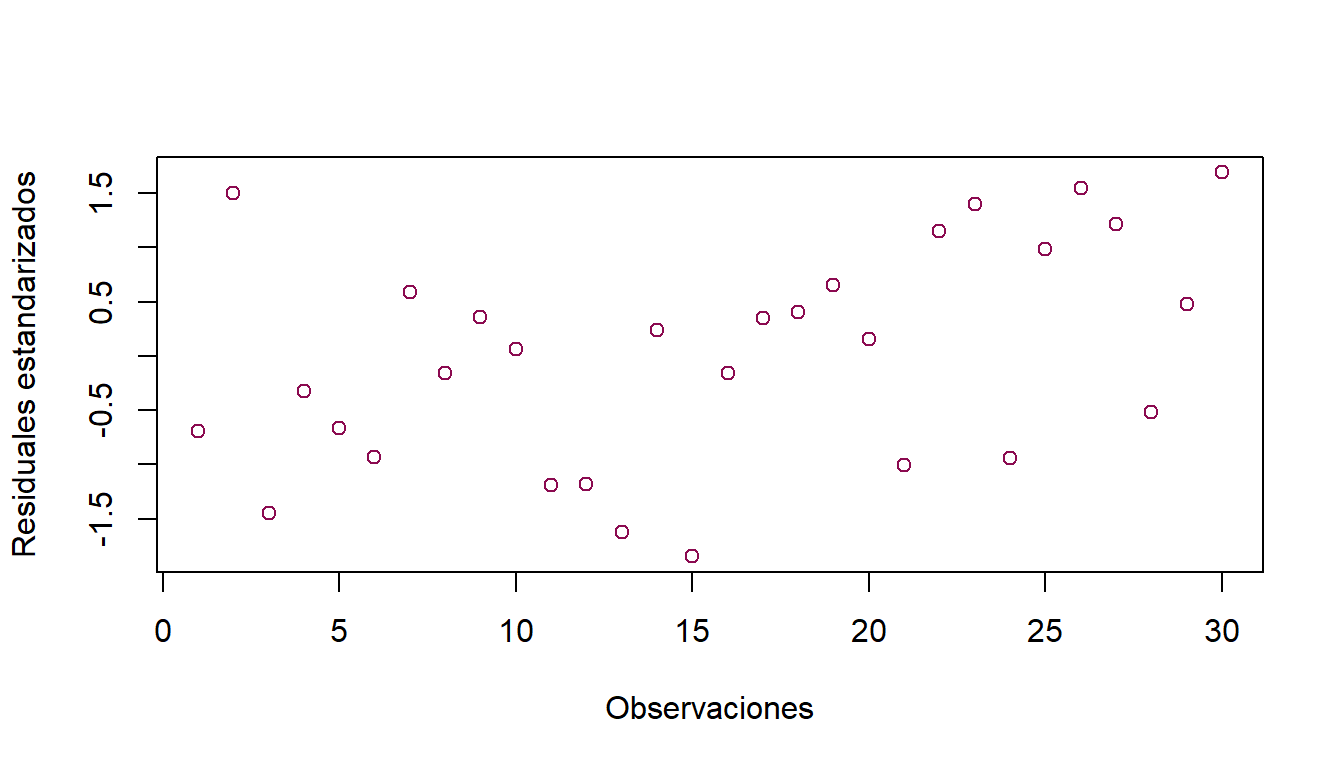
\includegraphics{_main_files/figure-latex/unnamed-chunk-43-1} \end{center}

\begin{itemize}
\tightlist
\item
  \(\textbf{Los residuales estudentizados}\)
\end{itemize}

\begin{Shaded}
\begin{Highlighting}[]
\FunctionTok{head}\NormalTok{(}\FunctionTok{rstudent}\NormalTok{(M1))}
\end{Highlighting}
\end{Shaded}

\begin{verbatim}
         1          2          3          4          5          6 
-0.6855868  1.5433247 -1.4786993 -0.3196249 -0.6557278 -0.9280596 
\end{verbatim}

\begin{Shaded}
\begin{Highlighting}[]
\FunctionTok{plot}\NormalTok{(}\FunctionTok{rstudent}\NormalTok{(M1),}\AttributeTok{col=}\StringTok{"deeppink4"}\NormalTok{,}\AttributeTok{ylab=}\StringTok{"Residuales estudentizados"}\NormalTok{, }\AttributeTok{xlab=}\StringTok{"Observaciones"}\NormalTok{)}
\end{Highlighting}
\end{Shaded}

\begin{center}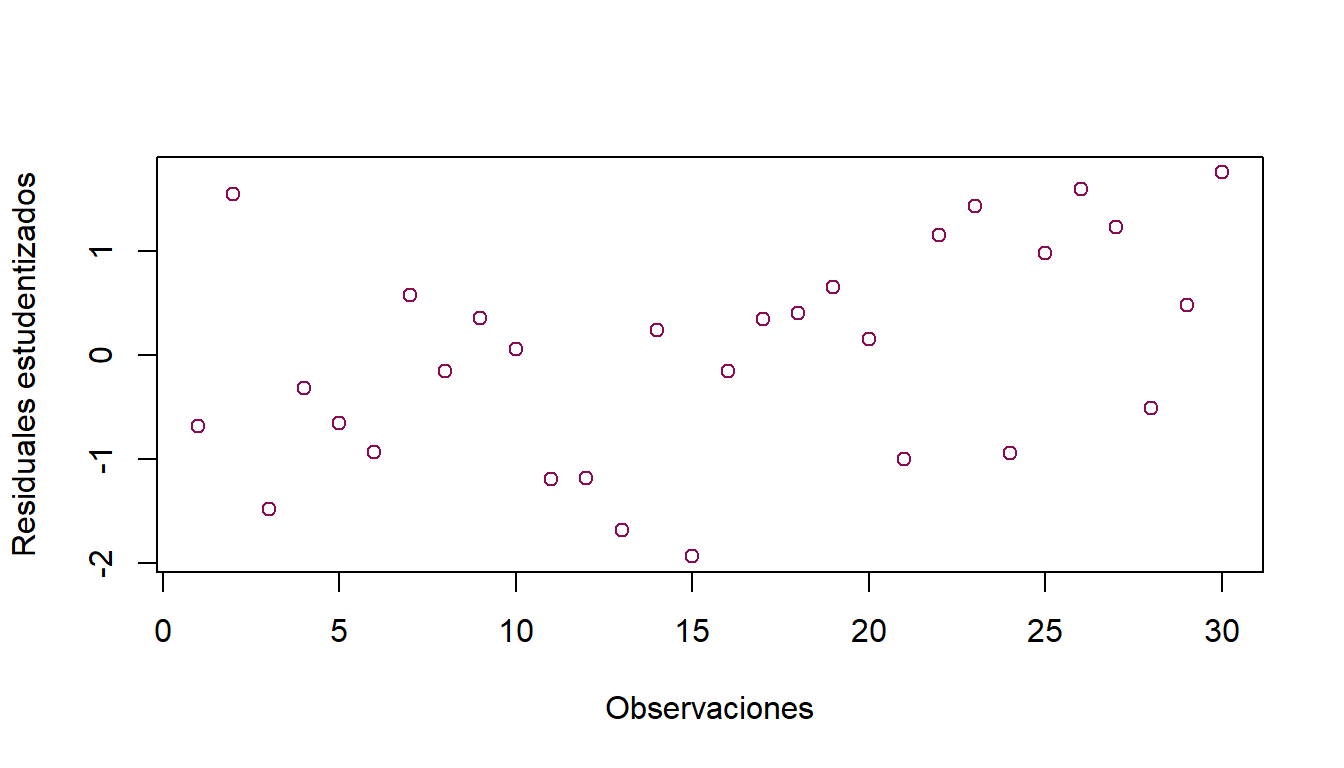
\includegraphics{_main_files/figure-latex/unnamed-chunk-45-1} \end{center}

\textbf{Validación de supuesto de normalidad}

Para validar gráficamente la normalidad de los errores debemos graficar los errores contra los cuantiles de la distribución normal. Para esto aplicaremos la función en R \textbf{qqnorm()} y con \textbf{qqline()} obtenemos la recta diagonal que nos servirá para ver que tan lejos o cerca de la distribución normal están cayendo los residuales del modelo.

\begin{Shaded}
\begin{Highlighting}[]
\FunctionTok{qqnorm}\NormalTok{(}\FunctionTok{rstandard}\NormalTok{(M1),}\AttributeTok{ylim =} \FunctionTok{c}\NormalTok{(}\SpecialCharTok{{-}}\DecValTok{2}\NormalTok{,}\DecValTok{2}\NormalTok{),}\AttributeTok{xlim =} \FunctionTok{c}\NormalTok{(}\SpecialCharTok{{-}}\DecValTok{2}\NormalTok{,}\DecValTok{2}\NormalTok{))}
\FunctionTok{qqline}\NormalTok{(}\FunctionTok{rstandard}\NormalTok{(M1),}\AttributeTok{distribution =}\NormalTok{ qnorm,}\AttributeTok{col=}\StringTok{"deeppink4"}\NormalTok{)}
\end{Highlighting}
\end{Shaded}

\begin{center}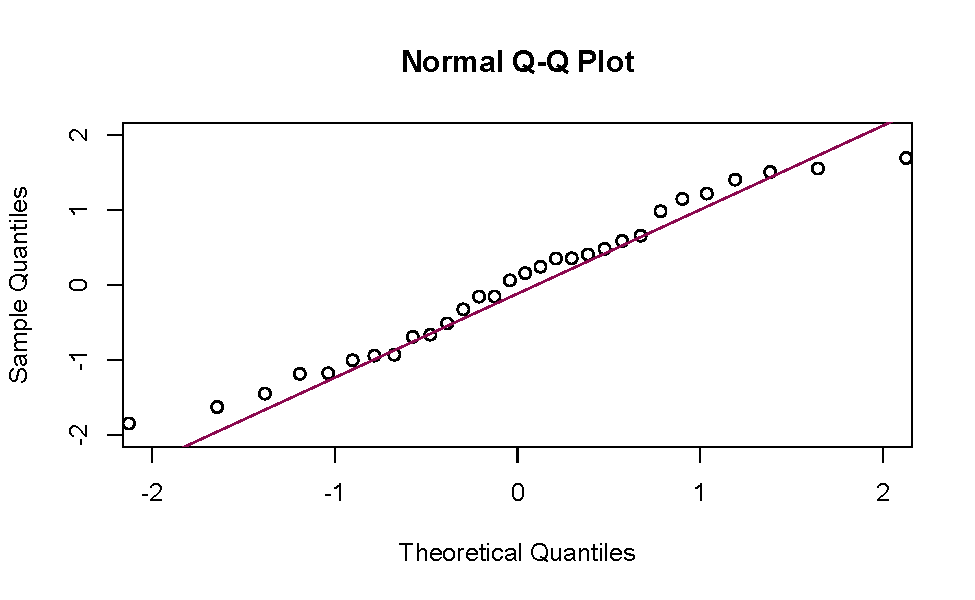
\includegraphics{_main_files/figure-latex/unnamed-chunk-46-1} \end{center}

Podemos observar que la parte central de la distribución si se ajusta a una distribución normal, sin embargo, en los extremos los residuales ya no se comportan como una distribución normal.

Podemos aplicar la prueba de bondad de ajuste \textbf{Lilliefors para normalidad} vista en Bondad de Ajuste:

\begin{Shaded}
\begin{Highlighting}[]
\NormalTok{nortest}\SpecialCharTok{::}\FunctionTok{ad.test}\NormalTok{(}\FunctionTok{rstandard}\NormalTok{(M1))}
\end{Highlighting}
\end{Shaded}

\begin{verbatim}

    Anderson-Darling normality test

data:  rstandard(M1)
A = 0.2675, p-value = 0.6615
\end{verbatim}

\begin{Shaded}
\begin{Highlighting}[]
\NormalTok{nortest}\SpecialCharTok{::}\FunctionTok{lillie.test}\NormalTok{(}\FunctionTok{rstandard}\NormalTok{(M1))}
\end{Highlighting}
\end{Shaded}

\begin{verbatim}

    Lilliefors (Kolmogorov-Smirnov) normality test

data:  rstandard(M1)
D = 0.088454, p-value = 0.7946
\end{verbatim}

Como el valor del \(p-value\) es mayor al nivel de significancia \(\alpha=0.05\) entonces no rechazamos \(H_{0}\), es decir nuestros residuales tienen distribución normal.

\textbf{Supuesto de linealidad}

El supuesto de linealidad lo verificamos gráficamente haciendo el diagrama de dispersión entre las variables como lo hicimos anteriormente.

\begin{center}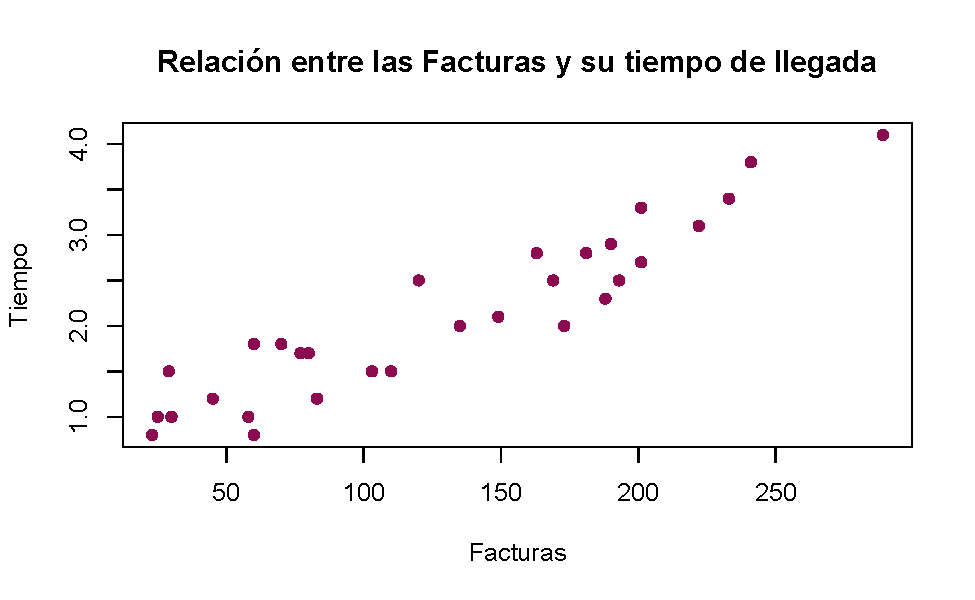
\includegraphics{_main_files/figure-latex/unnamed-chunk-48-1} \end{center}

Como lo mencionamos en su tiempo al observar nuestros datos nos grita que existe una relación lineal entre las variable facturas y tiempo empleado en ellas.

Como mencionamos en el capítulo, también se pueden graficar los errores estandarizados contra los valores observados de la variable explicativa.

\begin{center}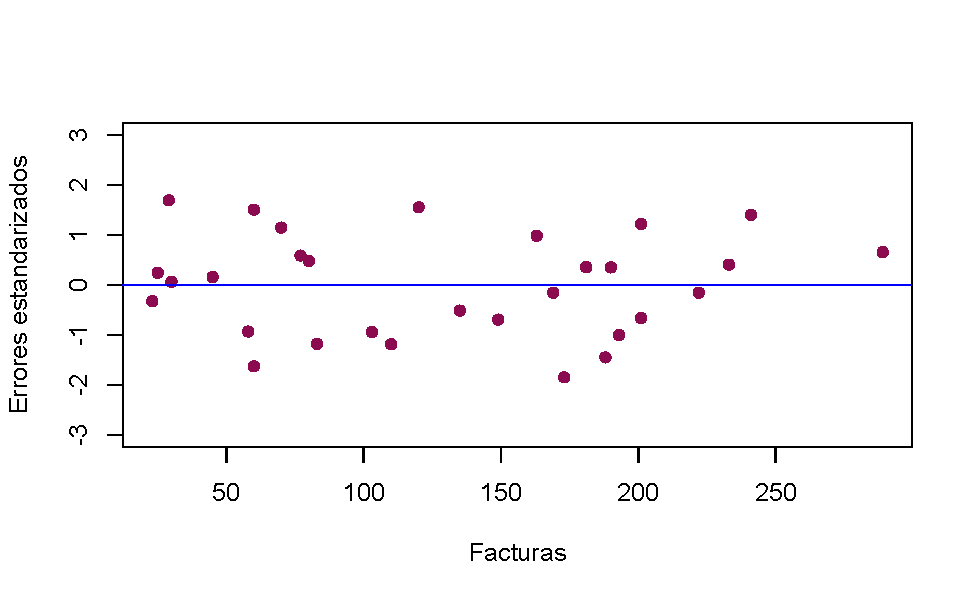
\includegraphics{_main_files/figure-latex/unnamed-chunk-49-1} \end{center}

En la gráfica anterior se observa un patrón aleatorio de los residuales estandarizados, esto indica que el modelo lineal es adecuado.

Un punto igual de importante es que no hay presencia de datos atípicos, ya que ningún residual está fuera de las bandas superior e inferior. Datos influyentes tampoco están presentes, pues no hay residuales que estén en alguna dirección lejana a los demás.

\textbf{Supuesto de Homocedasticidad}

Se dice que una muestra es homocedástica cuando la varianza es constante a lo largo de todas las observaciones, es decir, no varia conforme se presentan nuevas observaciones.

\begin{center}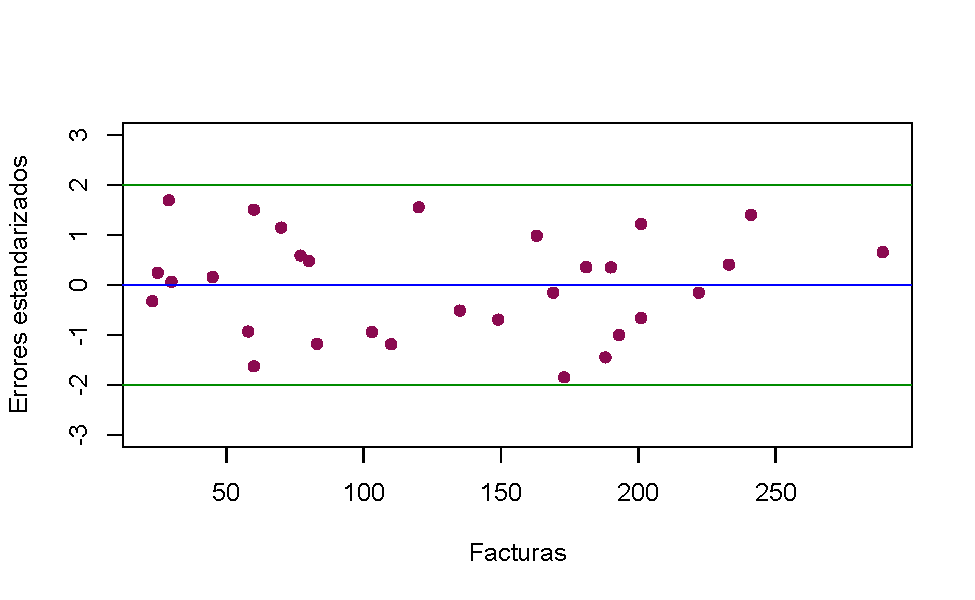
\includegraphics{_main_files/figure-latex/unnamed-chunk-50-1} \end{center}

\begin{itemize}
\tightlist
\item
  Si la varianza es constante entonces la gráfica fluctuaráentre el eje horizontal de manera simétrica, y sin seguir algún patrón, y se espera que la mayor parte de los errores estén contenidos en franjas horizontales delimitados por el eje entre -2 y 2. En éste ejemplo la dispersión regular de los residuales dentro de las Bandas superior e inferior y que no haya residuales que se alejen tanto de la Banda 0, indican varianza constante.
\end{itemize}

Adicionalmente aplicaremos las pruebas vistas en el capítulo para tener certeza estadística de la validez del supuesto de homocedasticidad.

\textbf{Prueba de Breusch-Pagan}

\begin{Shaded}
\begin{Highlighting}[]
\FunctionTok{bptest}\NormalTok{(M1)}
\end{Highlighting}
\end{Shaded}

\begin{verbatim}

    studentized Breusch-Pagan test

data:  M1
BP = 0.13226, df = 1, p-value = 0.7161
\end{verbatim}

El valor del \(p-value\) es mayor, por lo que la hipótesis de homocedasticidad no se rechaza.

\textbf{Prueba White}

\begin{verbatim}
[1] "Dia"      "Facturas" "Tiempo"  
\end{verbatim}

\begin{Shaded}
\begin{Highlighting}[]
\NormalTok{dataset}\OtherTok{=}\FunctionTok{data.frame}\NormalTok{(x, y)}
\NormalTok{model1}\OtherTok{=} \FunctionTok{VAR}\NormalTok{(dataset, }\AttributeTok{p =} \DecValTok{1}\NormalTok{)}
\CommentTok{\#whites.htest(model1)}
\end{Highlighting}
\end{Shaded}

El \(p-value\) es mayor, por lo que la hipótesis de homocedasticidad no se rechaza.

\textbf{Supuesto de No Correlación}

El estadístico de Durbin-Watson es una estadística de prueba que se utiliza para detectar la presencia de autocorrelación (una relación entre los valores separados el uno del otro por un intervalo de tiempo dado) en los residuales de un análisis de la regresión.

Las hipótesis que se plantean en la prueba de Durbin-Watson es:

\[\textbf{H}_0: \mbox{La autocorrelación de los residuales es igual a } 0 \ \ \  vs \ \ \  \textbf{H}_a: \mbox{La autocorrelación de los residuales es} \neq 0\]

En R se puede hacer la prueba de Durbin Watson con el comando \textbf{dwtest()}.

\begin{Shaded}
\begin{Highlighting}[]
\FunctionTok{dwtest}\NormalTok{(M1)}
\end{Highlighting}
\end{Shaded}

\begin{verbatim}

    Durbin-Watson test

data:  M1
DW = 1.7604, p-value = 0.2558
alternative hypothesis: true autocorrelation is greater than 0
\end{verbatim}

De acuerdo con el \(p-value\) los residuales no están correlacionados.

\textbf{Conclusiones}

Los supuestos hechos sobre los residuales se cumplen, por lo tanto el modelo propuesto es \textbf{totalmente adecuado} para \textbf{predecir} el tiempo promedio que tomará procesar un número de facturas dado:

\[\mbox{Tiempo promedio estimado}=0.6417+0.01129* \mbox{Número de Facturas Procesadas} \]
* \(\textbf{Puntos importantes}\)

\begin{enumerate}
\def\labelenumi{\arabic{enumi}.}
\item
  El gerente del departamento de ventas de \textbf{CALLCENT} podrá predecir el tiempo promedio en el que se procesará un número de facturas dado utilizando el modelo ajustado. Se sugiere realizar estimaciones dentro del rango de la dispersión de los datos, de lo contrario la variabilidad aumenta y podría tenerse estimaciones no tan precisas.
\item
  La ausencia de datos atípicos e influyentes indica que no hay factores que estén afectando el proceso de facturas y su tiempo empleado.
\item
  La cantidad de horas en la que tardarían en procesar una factura oscila en el intervalo (0.0096 hrs, 0.01296 hrs) a una confianza del 95\%. Puntualmente se estima que las horas requeridas para procesar una factura es 0.01129 hrs.
\end{enumerate}

4.- En este caso, el valor de \(\hat{\beta_{0}}\) (intercepto) no tiene una interpretación de acuerdo al contexto del problema.

\hypertarget{valores-outlier-e-influyentes}{%
\section{Valores outlier e influyentes}\label{valores-outlier-e-influyentes}}

Una vez que se ha verificado el cumplimiento de los supuestos en el modelo de regresión, se procede a examinar puntualmente cada observación en búsqueda de valores atípicos o de gran influencia en el modelo.

\hypertarget{valores-outlier}{%
\subsection{Valores outlier}\label{valores-outlier}}

Los valores atípicos, también conocidos por la terminología inglesa \(outlier\), son observaciones de la muestra aleatoria que no se comportan como el resto de los elementos que conforman el conjunto de datos, gráficamente, la observación con valor atípico no sigue la tendencia que de manera general sigue la muestra aleatoria, lo veremos en la siguiente figura, en el cual el punto rojo sobresale de toda la muestra marcada por puntos azules, por lo que la observación puede ser catalogada como un outlier o valor atípico.

\begin{center}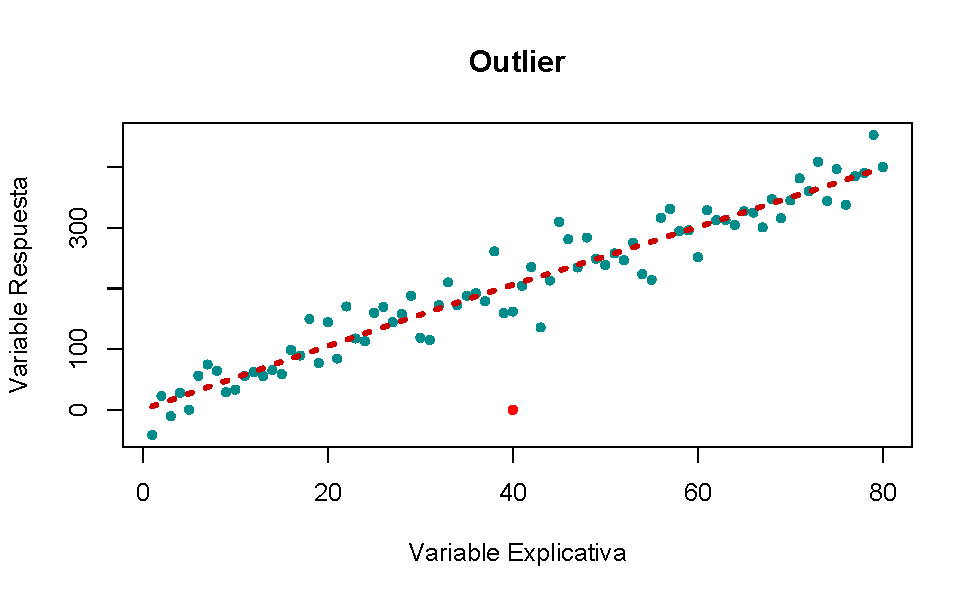
\includegraphics{_main_files/figure-latex/unnamed-chunk-55-1} \end{center}

Otra manera de detectar a los posibles valores atípicos es por medio de un análisis de residuales. Dicho análisis consiste en obtener los residuales, ya sean los estandarizados o estudentizados y observar si éstos son mayores o menores a comparación de un punto crítico con nivel de significancia \(\alpha\). Si se escoge trabajar con los residuales estandarizados sigue una distribución normal con media 0 y varianza \(\sigma^2\). Por lo que los residuales superiores o inferiores del punto crítico \(\pm Z_{1-\alpha/2}\) son considerados como un posible \(outlier\) con un nivel de significancia \(\alpha\). Por otra parte, si se decide trabajar con los residuales estudentizados entonces el punto crítico está determinado por los residuales que se encuentren por arriba o por abajo de la banda determinada por el cuantil \(\pm \ t_{1-\alpha/2,n-k-1}.\) Es decir, se tiene evidencia de un valor atípico con nivel de significancia \(\alpha\) cuando suceda alguna de las siguientes dos desigualdades:

\[\mid d_{i} \mid \geq Z_{1-\alpha/2}\]
\[\mid r_{i}\mid  \geq t_{1-\alpha/2,n-k-1}\]

Continuando con el ejemplo anterior, los posibles valores atípicos pueden ser visualizados en la siguiente figura, con un nivel de confianza del 99\%, y usando los residuales estandarizados para el análisis.

\begin{center}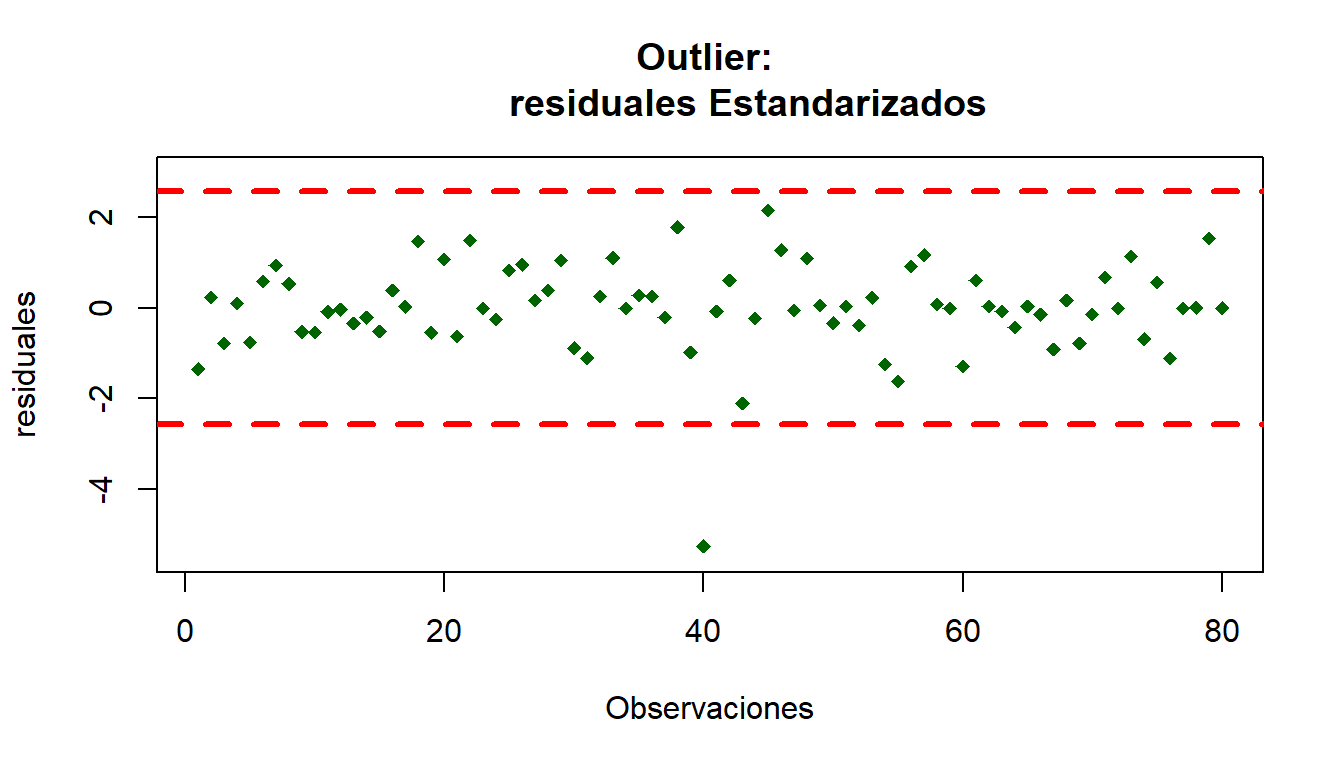
\includegraphics{_main_files/figure-latex/unnamed-chunk-56-1} \end{center}

Como se mencionó, es más que evidente que el punto atípico corresponde a la observación 40 la cual contrasta y sale de las bandas marcadas por el cuantil de la normal.

Generalmente se procede a eliminar observaciones atípicas, sin embargo, se recomienda realizar un análisis de influencia de las observaciones que presentan problemas de \(outlier\), ya que aunque se trata de puntos atípicos, puede resultar beneficioso para el modelo ya que puede que sean significativas para el modelo, por lo que eliminar estas observaciones puede ocasionar conflictos o desviaciones en la estimación.

\hypertarget{valores-influentes}{%
\subsection{Valores influentes}\label{valores-influentes}}

Los valores influentes, son observaciones que tienen una gran influencia en el ajuste del modelo, es decir, remover estas observaciones ocasionaría un cambio drástico en el modelo de regresión, ya que dichas observaciones tienen gran influencia en el cálculo de los estimadores de los parámetros o en las predicciones.

Es por esta propiedad por lo que se busca analizar estos puntos para medir su impacto en el modelo, para identificar si el \(outlier\) encontrado puede ser eliminado o no de la muestra.

Por ejemplo, imagine que tiene una muestra aleatoria conformada por 8 observaciones, en la cual 6 elementos son iguales y dos con diferente valor, tal como se muestra a continuación:

\begin{center}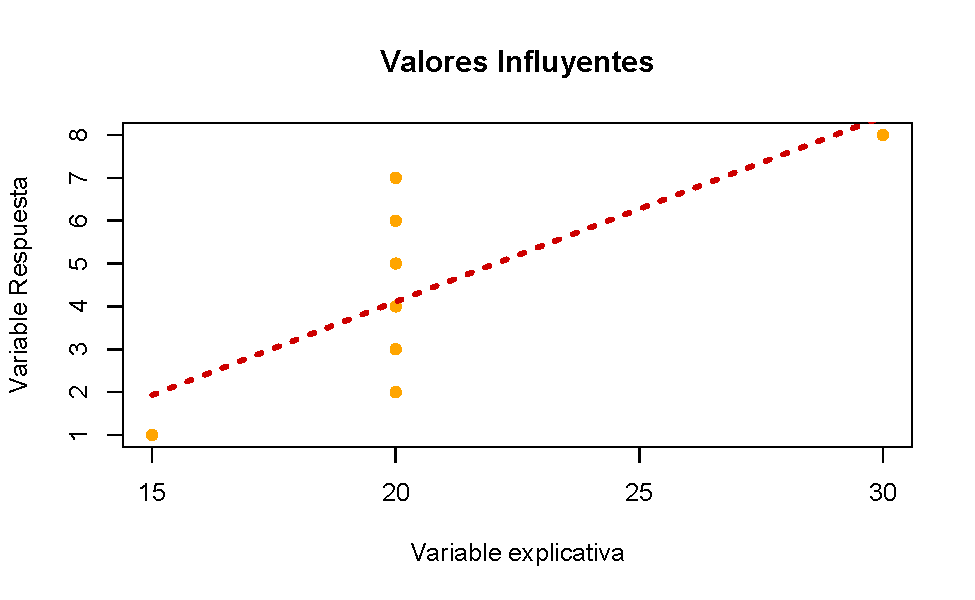
\includegraphics{_main_files/figure-latex/unnamed-chunk-57-1} \end{center}

El modelo tiene asociado una línea de regresión, sin embargo, si se quitan los extremos o valores atípicos, el modelo cambiaría rotundamente.

Un método para identificar la influencia del modelo es a través de los puntos palanca o leverage. El método consiste en examinar la medida entre el punto y el punto medio de los datos, a este punto también se le conoce como \(centroide\). Para ello se observa cuales son las observaciones influyentes examinando la matriz \(H\), o matriz sombrero, en el cual se pondrá especial atención a los elementos de la diagonal de la matriz \(H\), se denotará como \(h_{ii}\) al i-ésimo elemento de la diagonal \(H\), este último elemento se le denomina como el término de punto palanca o leverage.

Dado que el promedio de los valores leverage es \(\frac{\sum_{i=1}^{n}h_{ii}}{n},\) entonces cuando un punto sea mayor que el doble de la media de los puntos palanca, es decir, cuando se cumpla que:

\[h_{ii} \geq  2 \ \frac{\sum_{i=1}^{n}h_{ii}}{n}\]

Se puede concluir que dicha observación tiene un punto palanca muy grande. Por lo que se puede concluir que hay evidencia de que se trate de un punto influyente, sin embargo, para afirmar la anterior premisa es necesario el uso de otros métodos estadísticos, uno de ellos es la llamada distancia \textbf{Cook}.

La estadística de \textbf{Cook} propone calcular la distancia cuadrática entre el modelo ajustado y el modelo ajustado sin la \(i-ésima\) observación. La cual puede expresarse como:

\[C_{i}=\frac{\left(\underline{\hat{Y}}-\underline{\hat{Y}}_{(i)}\right)\left(\underline{\hat{Y}}-\underline{\hat{Y}}_{(i)}\right)}{CM_{error}\sum_{i=1}^{n}h_{ii}} \ \ \ \ \  \forall \ i \in [1,n].\]

Donde \(\underline{\hat{Y}}\) hace referencia al modelo ajustado de la forma \(X\underline{\hat{\beta}}\) mientras que \(\underline{\hat{Y}}_{(i)}\) hace referencia al modelo ajustado sin la i-ésima observación de forma \(X\underline{\hat{\beta}}_{(i)}\).

De esta manera, se calcula la distancia de \(Cook\) para cada observación, con la finalidad de evaluar el cambio del modelo sin la i-ésima observación. Se considera que una observación es influyente si el cambio del modelo con y sin observación varía mucho entre si, aunque no hay una medida establecida, (Hair, Tatham,Anderson y Black, 1998) sugiere que si la distancia de \(Cook\) de la i-ésima observación es mayor o igual a 1 se tiene evidencia de que la observación analizada tiene gran influencia en el modelo, mientras que para otros autores como (Bollen y Jackman, 1985) mencionan que las distancias mayores que \(\frac{4}{n}\) presenta indicios de influencia en el modelo.

\hypertarget{ejemplo-de-regresiuxf3n-lineal-simple}{%
\chapter{Ejemplo de regresión lineal simple}\label{ejemplo-de-regresiuxf3n-lineal-simple}}

A continuación veremos cómo resolver un problema que involucra ajustar un modelo de regresión lineal simple.

\hypertarget{contexto-del-problema}{%
\section{Contexto del problema}\label{contexto-del-problema}}

Para esta tarea usaremos los datos almacenados \href{https://raw.githubusercontent.com/alberto-mateos-mo/seminario-est-fciencias/master/datos/linear_regression_data/mmm_Rexample.csv}{aquí}.

Estos datos contienen información sobre el impacto que han tenido diferentes inversiones de publicidad en las ventas de la compañía.

El objetivo de la empresa es entender si las inversiones en publicidad por TV han beneficiado a las ventas y cuantificar este beneficio.

\hypertarget{exploraciuxf3n-de-datos}{%
\section{Exploración de datos}\label{exploraciuxf3n-de-datos}}

Para leer los datos directamente de GitHub usaremos la librería \texttt{readr}, la cual puede instalarse usando \texttt{install.packages("readr")}.

\begin{Shaded}
\begin{Highlighting}[]
\FunctionTok{library}\NormalTok{(readr)}
\FunctionTok{library}\NormalTok{(dplyr)}

\NormalTok{datos }\OtherTok{\textless{}{-}} \FunctionTok{read\_csv}\NormalTok{(}\StringTok{"https://raw.githubusercontent.com/alberto{-}mateos{-}mo/seminario{-}est{-}fciencias/master/datos/linear\_regression\_data/mmm\_Rexample.csv"}\NormalTok{)}

\FunctionTok{head}\NormalTok{(datos)}
\end{Highlighting}
\end{Shaded}

\begin{verbatim}
# A tibble: 6 x 5
  index    tv social_networks   ooh sales
  <dbl> <dbl>           <dbl> <dbl> <dbl>
1     1 230.             37.8  69.2  2210
2     2  44.5            39.3  45.1  1040
3     3  17.2            45.9  69.3   930
4     4 152.             41.3  58.5  1850
5     5 181.             10.8  58.4  1290
6     6   8.7            48.9  75     720
\end{verbatim}

Como podemos ver tenemos información de las ventas de la compañía y de los montos que se han destinado para publicidad en televisión (tv), redes sociales (social\_networks) y exteriores (ooh).

Seleccionaremos, en este las variables correspondientes a ventas e inversiones en TV

\begin{Shaded}
\begin{Highlighting}[]
\NormalTok{datos }\OtherTok{\textless{}{-}}\NormalTok{ datos }\SpecialCharTok{\%\textgreater{}\%} 
\NormalTok{  dplyr}\SpecialCharTok{::}\FunctionTok{select}\NormalTok{(sales, tv)}
\end{Highlighting}
\end{Shaded}

\hypertarget{visualizaciuxf3n-de-datos}{%
\section{Visualización de datos}\label{visualizaciuxf3n-de-datos}}

Crearemos un gráfico de dispersión entre las variables seleccionadas buscando evidencia de algun tipo de relación entre las ventas y las inversiones en TV.

A este gráfico le agregaremos el coeficiente de correlación entre las variables.

\begin{Shaded}
\begin{Highlighting}[]
\FunctionTok{library}\NormalTok{(ggplot2)}

\FunctionTok{ggplot}\NormalTok{(datos, }\FunctionTok{aes}\NormalTok{(tv, sales))}\SpecialCharTok{+}
  \FunctionTok{geom\_point}\NormalTok{()}\SpecialCharTok{+}
  \FunctionTok{ggtitle}\NormalTok{(}\AttributeTok{label =} \StringTok{"Relación entre ventas e inversiones en TV"}\NormalTok{,}
          \AttributeTok{subtitle =} \FunctionTok{paste}\NormalTok{(}\StringTok{"Coeficiente de correlación:"}\NormalTok{, }
                           \FunctionTok{round}\NormalTok{(}\FunctionTok{cor}\NormalTok{(datos}\SpecialCharTok{$}\NormalTok{tv, datos}\SpecialCharTok{$}\NormalTok{sales), }\DecValTok{2}\NormalTok{)))}\SpecialCharTok{+}
  \FunctionTok{theme\_minimal}\NormalTok{()}
\end{Highlighting}
\end{Shaded}

\begin{center}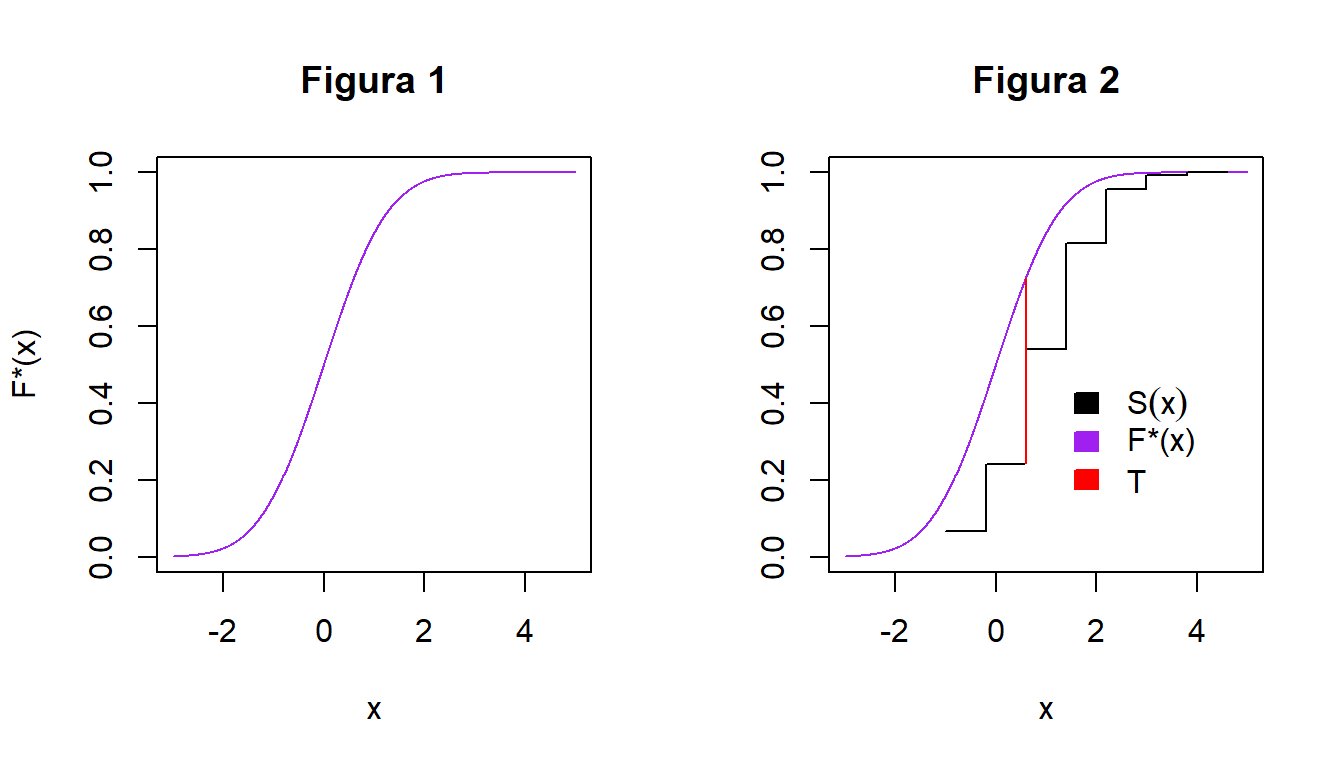
\includegraphics{_main_files/figure-latex/unnamed-chunk-60-1} \end{center}

En este grafico podemos identificar la existencia de una relación directamente proporcional entre los montos invertidos en TV y las ventas, lo cual se confirma con el coeficiente de correlación.

Recordemos que justamente uno de los supuestos del modelo de regresión lineal simple es que debe existir una relación lineal entre las variables independiente y dependiente.

\hypertarget{ajuste-del-modelo-de-regresiuxf3n-lineal-simple}{%
\section{Ajuste del modelo de regresión lineal simple}\label{ajuste-del-modelo-de-regresiuxf3n-lineal-simple}}

Con este modelo encontraremos la ecuación de la recta que mejor describa la relación entre nuestras dos variables de interés.

Recordemos que esta recta estará descrita de la siguiente forma:

\[sales = \beta_0 + \beta_1*tv\]

\begin{Shaded}
\begin{Highlighting}[]
\NormalTok{modelo }\OtherTok{\textless{}{-}} \FunctionTok{lm}\NormalTok{(sales }\SpecialCharTok{\textasciitilde{}}\NormalTok{ tv, }\AttributeTok{data =}\NormalTok{ datos)}
\end{Highlighting}
\end{Shaded}

\hypertarget{validaciuxf3n-del-modelo}{%
\section{Validación del modelo}\label{validaciuxf3n-del-modelo}}

Mediante el resumen del modelo tendremos acceso a todas las métricas necesarias para evaluar qué tan \emph{bueno} es.

\begin{Shaded}
\begin{Highlighting}[]
\FunctionTok{summary}\NormalTok{(modelo)}
\end{Highlighting}
\end{Shaded}

\begin{verbatim}

Call:
lm(formula = sales ~ tv, data = datos)

Residuals:
    Min      1Q  Median      3Q     Max 
-838.60 -195.45  -19.13  206.71  721.24 

Coefficients:
            Estimate Std. Error t value Pr(>|t|)    
(Intercept) 703.2594    45.7843   15.36   <2e-16 ***
tv            4.7537     0.2691   17.67   <2e-16 ***
---
Signif. codes:  0 '***' 0.001 '**' 0.01 '*' 0.05 '.' 0.1 ' ' 1

Residual standard error: 325.9 on 198 degrees of freedom
Multiple R-squared:  0.6119,    Adjusted R-squared:  0.6099 
F-statistic: 312.1 on 1 and 198 DF,  p-value: < 2.2e-16
\end{verbatim}

En primer lugar veremos la sección \textbf{Call}, en esta sección se describe qué modelo se esta ajustando; esta parte es meramente informativa.

La sección \textbf{Residuals} nos da una idea de la distribución de los residuales.

\textbf{Para pensar: ¿por qué el resumen del modelo omite la media de los residuales?, ¿qué deberíamos esperar de la mediana?}

\hypertarget{coefficients}{%
\subsection{Coefficients}\label{coefficients}}

En la tabla de esta sección se muestran:

\begin{itemize}
\item
  Los estimadores de los coeficientes del modelo i.e.~\(\beta_0\) (Intercept) y \(\beta_1\) (tv)
\item
  Los errores estandar para los coeficientes
\item
  El estadístico t y el p-value correspondiente: estos definen la significancia estadística de los estimadores
\end{itemize}

De este ejemplo podemos concluir que ambos coeficientes son significativos, es decir, hay una asociación entre las inversiones en TV y las ventas.

\hypertarget{bondad-de-ajuste}{%
\section{Bondad de ajuste}\label{bondad-de-ajuste}}

La última sección nos muestra:

\begin{itemize}
\item
  El error estándar de los residuales: representa las variaciones de los datos reales en torno a la linea de regresión ajustada por el modelo.
\item
  R cuadrada y R cuadrada ajustada: representan la proporción de información de los datos que es explicada por el modelo. La diferencia entre ellas es que la R cuadrada ajustada considera en su cálculo una penalización por la cantidad de parámetros que estima el modelo.
\item
  Estadístico F: evalua si al menos una variable independiente tiene coeficiente distinto de cero; este estadístico será útil cuando apliquemos modelos multivariados.
\end{itemize}

\hypertarget{intepretaciuxf3n-de-resultados}{%
\section{Intepretación de resultados}\label{intepretaciuxf3n-de-resultados}}

Una vez validado el modelo de regresión lineal simple podemos usar sus resultados para intepretarlos en el contexto del problema.

Recordemos que nuestro objetivo es entender si las inversiones en publicidad por TV han beneficiado a las ventas y cuantificar este beneficio.

En primer lugar podemos determinar que las inversiones en publicidad por televisión sí influyen en el desempeño de las ventas.

El coeficiente \(\beta_0\) (Intercept) nos indica las ventas promedio generadas por otros factores no medidos y con inversiones nulas en TV.

El coeficiente \(\beta_1\) asociado a las inversiones en TV nos da el incremento (dado que es positivo) promedio en ventas por cada incremento de una unidad monetaria en TV.

Es decir, las inversiones en publicidad por TV benefician a las ventas, generando en promedio \textasciitilde5 unidades monetarias de venta por cada unidad monetaria invertida en este medio.

\hypertarget{part-modelo-de-regresiuxf3n-lineal-muxfaltiple}{%
\part{Modelo de regresión lineal múltiple}\label{part-modelo-de-regresiuxf3n-lineal-muxfaltiple}}

\hypertarget{introducciuxf3n-1}{%
\chapter*{Introducción}\label{introducciuxf3n-1}}


El modelo de regresión lineal simple ajusta una variable explicativa a una variable respuesta; Por su parte, el \textbf{Modelo de regresión lineal múltiple} busca hallar el mejor ajuste con dos o más variables regresoras. Es decir, la variable respuesta \(\underline{Y}\) depende de \(k\) regresores de la forma:

\[
\underline{Y}=\beta_{0}+\beta_{1}x_{1}+\beta_{2}x_{2}+ \ldots +\beta_{k}x_{k}+\epsilon
\]

En primera instancia no parece ser un gran cambio, sin embargo, es de gran importancia ya que de esta forma se puede estimar de una mejor manera un evento aleatorio, pues en general, un suceso no depende de sólo una acción o variable, sino que es resultado de una serie de diversos eventos o variables.

Es importante mencionar que en un modelo de regresión múltiple se deja de ajustar una línea recta a los datos, en cambio se ajusta un hiperplano.

\begin{center}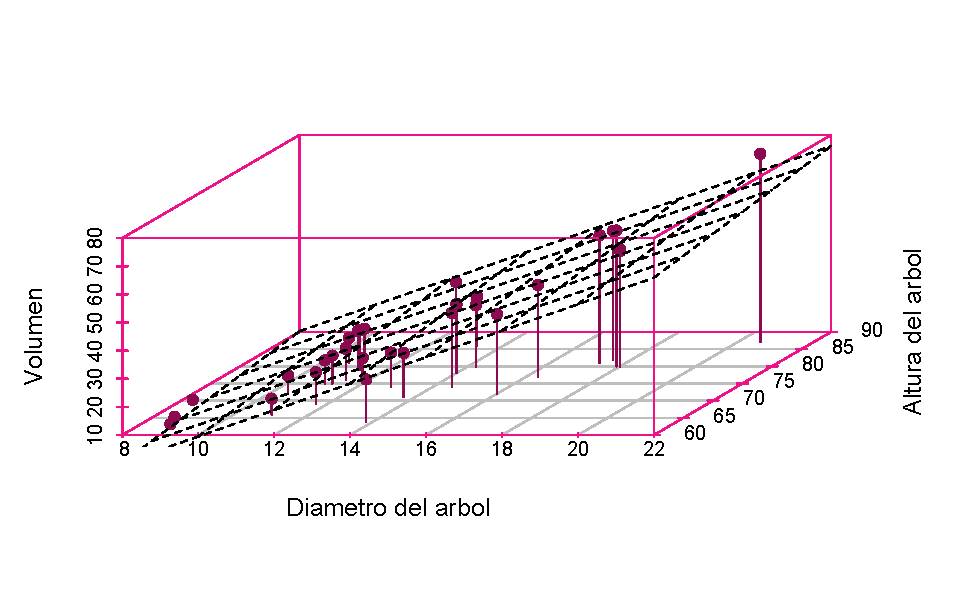
\includegraphics{_main_files/figure-latex/unnamed-chunk-63-1} \end{center}

El ``scatterplot'' de arriba, se realizó con la base precargada en \(R\), \("trees"\), los datos que componen la muestra se encuentran en un vector de dimensión 3, la cual busca relacionar la variable \(\underline{Y}\), con dos variables explicativas \(X_{1}\) y \(X_{2}\), en este caso, la variable \(\underline{Y}\) hace referencia al volumen de un árbol y la variable \(X_{1}\) hace referencia al diámetro del tronco del árbol y \(X_{2}\) denota la altura del árbol, se observa que existe una tendencia, la cual es representada mediante el hiperplano de regresión marcado, en la cual a menor diámetro y menor altura, el volumen del árbol tiende a disminuir.

Debido a que se trabaja con cierto error \(\epsilon\) en el ajuste de la regresión, es conveniente suponer que se cumplen lo siguientes supuestos:

\textbf{Definición 3.1} (Supuestos del modelo de regresión múltiple)

El error \(\epsilon_{i}\) en el modelo de regresión lineal múltiple cumple:

\begin{itemize}
\item
  \(\mathbf{E}[\epsilon_{i}]=0.\)
\item
  \(Var(\epsilon_{i})=\sigma^2.\)
\item
  \(Cov(\epsilon_{i},\epsilon_{j})=0, \ \ i \neq j \ \ \forall \ \ i= 1,2,\ldots,n; \ \ j= 1,2,\ldots,n.\)
\end{itemize}

Al cumplirse estos supuestos es posible calcular la esperanza y varianza de la variable respuesta \(\underline{Y}\) dado un conjunto de valores \(x_{1},x_{2},\ldots,x_{k}.\)

\textbf{Teorema 3.1} Sea una variable de interés \(\underline{Y}\), llamada \textbf{dependiente}, relacionada con dos o más variables explicativas o también llamadas regresoras \(x_{1},x_{2},\ldots,x_{k}\),
entonces:

\textbf{a)} \(\mathbf{E}[\underline{Y}]= \beta_{0}+\beta_{1}x_{1}+\beta_{2}x_{2}+ \ldots + \beta_{k}x_{k}.\)

\textbf{b)} \(\textbf{Var}(\underline{Y})= \sigma^2.\)

\textbf{Demostración:}

\textbf{a)} Para la esperanza de \(\underline{Y}\) se tiene:

\[\mathbf{E}[\underline{Y}]=\mathbf{E}[\beta_{0}+\beta_{1}x_{1}+\beta_{2}x_{2}+ \ldots +\beta_{k}x_{k}+\epsilon].\]
La estimación es sobre \(\underline{Y},\)
como \(\beta_{0},\beta_{1},\beta_{2},\ldots,\beta_{k}\) son constantes; \(x_{1},x_{2}, \ldots,x_{k}\) son los valores dados, por lo que:

\[\mathbf{E}[\underline{Y}]=\beta_{0}+\beta_{1}x_{1}+\beta_{2}x_{2}+ \ldots +\beta_{k}x_{k}+\mathbf{E}[\epsilon].\]

\[=\beta_{0}+\beta_{1}x_{1}+\beta_{2}x_{2}+ \ldots +\beta_{k}x_{k}+0\]
\[\therefore \mathbf{E}[\underline{Y}]= \beta_{0}+\beta_{1}x_{1}+\beta_{2}x_{2}+ \ldots + \beta_{k}x_{k}. \blacksquare\]

\textbf{b)} Para la varianza de \(\underline{Y}\) se tiene:

\[Var(\underline{Y})=Var\left( \beta_{0}+\beta_{1}x_{1}+\beta_{2}x_{2}+ \ldots + \beta_{k}x_{k}+ \epsilon\right).\]
La estimación es sobre \(\underline{Y}\), \(\beta_{0},\beta_{1},\beta_{2},\ldots,\beta_{k}\) son constantes;~\(x_{1},x_{2},\ldots,x_{k}\) son valores dados, por lo que cumple que:

\[Var(\underline{Y})=0+0+0+\ldots+0+Var(\epsilon)\]
\[\therefore Var(\underline{Y})=\sigma^2.\blacksquare\]

\hypertarget{modelo}{%
\chapter{Modelo}\label{modelo}}

El objetivo del modelo de regresión lineal múltiple consiste en modelar \(\underline{Y}\) a través de \(k\) variables regresoras en \(n\) observaciones independientes. Es decir, se tiene el siguiente modelo:

\[
\begin{array}{ c c c c c c c c c c c c c }
Y_{1}  & = & \beta_{0} & + & \beta_{1}x_{11}& +& \beta_{2}x_{12} & +& \cdots & + & \beta_{k}x_{1k} & + & \epsilon_{1}  \\ 
Y_{2}  & = & \beta_{0} & + & \beta_{1}x_{21}& +& \beta_{2}x_{22} & +& \cdots & + & \beta_{k}x_{2k} & + & \epsilon_{2}  \\
\vdots  &  & \vdots &  & \vdots& & \vdots & & \vdots & & \vdots &  & \vdots  \\
Y_{n}  & = & \beta_{0} & + & \beta_{1}x_{n1}& +& \beta_{2}x_{n2} & +& \cdots & + & \beta_{k}x_{nk} & + & \epsilon_{n}  \\ 
\end{array}
\]

El anterior conjunto de igualdades puede ser denotado matricialmente mediante la siguiente igualdad:

\[\underline{Y}=X\underline{\beta}+\underline{\epsilon}\]

donde:
\[
\underline{Y}=
\left(
\begin{array}{c}
y_{1} \\
y_{2} \\
\vdots \\
y_{n}\\
\end{array}
\right),\ \ \ \  X=
\left(
\begin{array}{c c c c c}
1      & x_{11} & x_{12} & \ldots & x_{1k}\\ 
1      & x_{21} & x_{22} & \ldots & x_{2k}\\
\vdots & \vdots & \vdots & \ddots & \vdots\\
1      & x_{n1} & x_{n2} & \ldots & x_{nk}\\
\end{array}
\right)
\]
\[
\underline{\beta}=
\left(
\begin{array}{c}
\beta_{0} \\
\beta_{1} \\
\vdots \\
\beta_{k}\\
\end{array}
\right),\ \ \ \  \epsilon=
\left(
\begin{array}{c}
\epsilon_{1} \\
\epsilon_{2} \\
\vdots \\
\epsilon_{n}\\
\end{array}
\right)
\]
Sustituyendo en la ecuación anterior, se observa que el modelo de regresión multiple puede ser visto como:
\[
\left(
\begin{array}{c}
y_{1} \\
y_{2} \\
\vdots \\
y_{n}\\
\end{array}
\right)=
\left(
\begin{array}{c c c c c}
1      & x_{11} & x_{12} & \ldots & x_{1k}\\ 
1      & x_{21} & x_{22} & \ldots & x_{2k}\\
\vdots & \vdots & \vdots & \ddots & \vdots\\
1      & x_{n1} & x_{n2} & \ldots & x_{nk}\\
\end{array}
\right)
\left(
\begin{array}{c}
\beta_{0} \\
\beta_{1} \\
\vdots \\
\beta_{k}\\
\end{array}
\right) + 
\left(
\begin{array}{c}
\epsilon_{1} \\
\epsilon_{2} \\
\vdots \\
\epsilon_{n}\\
\end{array}
\right)
\]

La dimensión de las matrices señaladas anteriormente se mencionan en el siguiente recuadro:

\[
\begin{array}{|c|c|}
\hline
Matriz & Dimensión \\
\hline
\underline{Y}        & n \times 1 \\
X                   & n \times (k+1) \\
\underline{\epsilon} & n \times 1 \\
\underline{\beta}    & (k+1) \times 1 \\
\hline
\end{array}
\]

Finalmente para definir correctamente el modelo es necesario realizar las siguientes suposiciones acerca de las matrices del modelo de regresión lineal múltiple.

\textbf{Definición 3.2} Sea \(X\) la denominada \(matriz \ diseño\) entonces satisface que:

\begin{itemize}
\tightlist
\item
  \(X_{n \times (k+1)}\) es el rango completo en la columna, es decir, \(X\) es de rango \(k+1\)
\end{itemize}

Éste supuesto es importante ya que satisface que \(k+1\leq n\), es decir, \textbf{el máximo número de variables con el que se ajusta el modelo no puede ser superior al número de observaciones.}

De igual forma, observe que el supuesto de la varianza de los errores en la \textbf{definición 3.1}, puede reescribirse en forma matricial:

\[
Var(\epsilon)=
\left(
\begin{array}{c c c c c}
Var(\epsilon_{1}) & Cov(\epsilon_{1},\epsilon_{2}) & Cov(\epsilon_{1},\epsilon_{3}) & \ldots & Cov(\epsilon_{1},\epsilon_{ n})\\ 
Cov(\epsilon_{2},\epsilon_{1})&Var(\epsilon_{2}) & Cov(\epsilon_{2},\epsilon_{3}) & \ldots &Cov(\epsilon_{2},\epsilon_{n}) \\
\vdots & \vdots & \vdots & \ddots & \vdots\\
Cov(\epsilon_{n},\epsilon_{1})   & Cov(\epsilon_{n},\epsilon_{2}) & Cov(\epsilon_{n},\epsilon_{3}) & \ldots & Var(\epsilon_{n})\\
\end{array}
\right)
\]

Por \textbf{definición 3.1}, \(Cov(\epsilon_{i},\epsilon_{j})=0 \ \ \ i\neq j\)

\[
Var(\epsilon)=
\left(
\begin{array}{c c c c c}
Var(\epsilon_{1}) & 0 & 0 & \ldots & 0 \\ 
0&Var(\epsilon_{2}) & 0 & \ldots & 0 \\
\vdots & \vdots & \vdots & \ddots & \vdots\\
0 & 0 & 0 & \ldots & Var(\epsilon_{n})\\
\end{array}
\right)
\]

Por \textbf{definición 3.1}, \(Var(\epsilon_{i})=\sigma^2\)

\[
Var(\epsilon)=
\left(
\begin{array}{c c c c c}
\sigma^2 & 0 & 0 & \ldots & 0 \\ 
0&\sigma^2 & 0 & \ldots & 0 \\
\vdots & \vdots & \vdots & \ddots & \vdots\\
0 & 0 & 0 & \ldots &\sigma^2  \\
\end{array}
\right)
\]

\(\therefore Var(\epsilon)=\sigma^2 I_{n \times n}. \blacksquare\)

\hypertarget{estimaciuxf3n-por-muxednimos-cuadrados-de-los-paruxe1metros-del-modelo-2}{%
\section{Estimación por mínimos cuadrados de los parámetros del modelo}\label{estimaciuxf3n-por-muxednimos-cuadrados-de-los-paruxe1metros-del-modelo-2}}

Es necesario dar una estimación de la intersección con el eje \(\underline{Y}\), las variables que conforman el hiperplano, es decir, \(\beta_{0},\beta_{1},\beta_{2},\ldots,\beta_{k}\) respectivamente. La manera en la que se construyen a los estimadores es tal que la diferencia entre todos los valores observados y los valores estimados sea 0, es decir, a éstas diferencias se le conoce como \(\mathbf{residuales}\), muchos autores también hacen referencia a ellos como \(\mathbf{residuos}\).

\textbf{Definición 3.3} (Residuales). Sea \(y_{i}\) los valores observados, y sea \(\hat{y}_{i}\) los valores ajustados de la forma \(\hat{y}_{i}=\hat{\beta_{0}}+\hat{\beta_{1}}x_{1i}+\hat{\beta_{2}}x_{2i}+ \ldots +\hat{\beta_{k}}x_{ki}\) ~para ~\(\hat{\beta_{0}},\hat{\beta_{1}},\hat{\beta_{2}}, \ldots, \hat{\beta_{k}}\) ~dados, ~entonces:

\[e_{i}=y_{i}-\hat{y_{i}} \ \ \ \ \ \ i=1, \ldots,n.\]
Se les conoce como \textbf{residuales.}

Para estimar los valores desconocidos \(\beta_{0},\beta_{1},\beta_{2},\ldots,\beta_{k}\) se usa el \textbf{método de mínimos cuadrados}, el cual es similar al caso de regresión lineal simple, dicho método propone minimizar la suma de cuadrados de los residuales.

Antes de continuar es necesario ver algunos resultados importantes de equivalencia y notación.

De la \textbf{definición 3.3} se sabe que los valores esperados de \(y_{i}\) pueden ser definidos como:

\[
\begin{array}{c}
\hat{y_{1}} \\
\hat{y_{2}} \\
\vdots \\
\hat{y_{n}}\\
\end{array}
\begin{array}{c c c c c c c c c c}
=&\hat{\beta_{0}}&+&\hat{\beta_{1}} x_{11} &+& \hat{\beta_{2}}x_{12}&+& \ldots &+&\hat{\beta_{k}} x_{1k}\\ 
=&\hat{\beta_{0}}&+&\hat{\beta_{1}} x_{21} &+& \hat{\beta_{2}}x_{22}&+& \ldots &+&\hat{\beta_{k}} x_{2k}\\ 
&\vdots && \vdots && \vdots && \vdots && \vdots\\
=&\hat{\beta_{0}}&+&\hat{\beta_{1}} x_{n1} &+& \hat{\beta_{2}}x_{n2}&+& \ldots &+&\hat{\beta_{k}} x_{nk}\\ 
\end{array}
\]

La anterior ecuación puede ser descompuesta en forma matricial de la siguiente manera:

\[
\left(
\begin{array}{c}
\hat{y_{1}} \\
\hat{y_{2}} \\
\vdots \\
\hat{y_{n}}\\
\end{array}
\right)=
\left(
\begin{array}{c c c c c}
1      & x_{11} & x_{12} & \ldots & x_{1k}\\ 
1      & x_{21} & x_{22} & \ldots & x_{2k}\\
\vdots & \vdots & \vdots & \ddots & \vdots\\
1      & x_{n1} & x_{n2} & \ldots & x_{nk}\\
\end{array}
\right)
\left(
\begin{array}{c}
\hat{\beta_{0}} \\
\hat{\beta_{1}} \\
\vdots \\
\hat{\beta_{k}}\\
\end{array}
\right)
\]

Por lo tanto, podemos renombrar a las matrices de acuerdo a los elementos que las conforman.

Se tiene la siguiente igualdad para los valores estimados \(\underline{\hat{Y}}.\)

\[\underline{\hat{Y}}=X \underline{\hat{\beta}}.\]

Ahora por la \textbf{definición 3.3} y lo anterior tenemos que los residuales se encuentran de la forma:

\[\underline{e}=\underline{Y}-X \underline{\hat{\beta}}.\]

\textbf{Teorema 3.2} (Mínimos Cuadrados).(MC) Si se minimiza la suma de cuadrados de la diferencia entre los valores observados y los estimados, la cual se expresa matricialmente de la siguiente forma:

\[\underline{e'}\underline{e}.\]

Entonces se tiene como estimador de \(\underline{\beta}\) a:

\[\underline{\hat{\beta}}=\left( X'X\right)^{-1}X'\underline{Y}.\]

\textbf{Demostración:}

Se sabe que los residuales están definidos como \(\underline{e}=\left( \underline{Y}-X \underline{\hat{\beta}}\right)\) de esta manera, por hipótesis se tiene:

\[\underline{e'}\underline{e}=\left( \underline{Y}-X \underline{\hat{\beta}}\right)'\left( \underline{Y}-X \underline{\hat{\beta}}\right).\]
\[=\left(\underline{Y}'- \underline{\hat{\beta}}'X'\right)\left( \underline{Y}-X \underline{\hat{\beta}}\right).\]
\[=\underline{Y}'Y-\underline{Y}'X\underline{\hat{\beta}}-\underline{\hat{\beta}}'X'\underline{Y}+\underline{\hat{\beta}}'X'X\underline{\hat{\beta}}.\]
\[\underline{e'}\underline{e}=\underline{Y}'Y-2\underline{Y}'X\underline{\hat{\beta}}+\underline{\hat{\beta}}'X'X\underline{\hat{\beta}}.\]
Lo anterior se da ya que \(\underline{\hat{\beta}}'X'\underline{Y}\) es una matriz de \(1\times 1\), es decir, un escalar, y que su transpuesta \((\underline{\hat{\beta}}'X'\underline{Y})'=\underline{Y}'X\underline{\hat{\beta}}\) es el mismo escalar.

Derivando respecto a \(\underline{\hat{\beta}}\) para hallar los posibles mínimos se divide la suma matricial de la siguiente forma:

\[\Delta \underline{\hat\beta}=\Delta_{1} \underline{\hat{\beta}}+\Delta_{2} \underline{\hat{\beta}}+\Delta_{3} \underline{\hat{\beta}}\]

Procederemos a derivar:

\[
\Delta\underline{\hat{\beta}}=\left\{
\begin{array}{ll}
\Delta_{1} \underline{\hat{\beta}} \ \ \ \ \ \left(\underline{Y}'\underline{Y}\right)  \ \ \ \ \ \ \ \ =0 \\
\Delta_{2} \underline{\hat{\beta}} \ \ \ \ \left( -2\underline{Y}'X\underline{\hat{\beta}}\right) \ \ = \left(-2\underline{Y}'X\right)'=-2X'\underline{Y} \\
\Delta_{3} \underline{\hat{\beta}} \ \  \ \ \left( \underline{\hat{\beta}'}X'X\underline{\hat{\beta}}\right)  \ \ \ = 2X'X\underline{\hat{\beta}}
\end{array}
\right. 
\]

De esta forma se tiene que la derivada respecto a \(\underline{\beta}\) es:

\[\Delta \underline{\beta}=-2X'\underline{Y}+2X'X\underline{\hat{\beta}}.\]
Igualamos la derivada a 0, para hallar un punto crítico:

\[\Delta \underline{\hat{\beta}}=0\]
\[-2X'\underline{Y}+2X'X\underline{\hat{\beta}}=0\]
\[2X'X\underline{\hat{\beta}}=2X'\underline{Y}\]
Esto se simplifica a:

\[X'X\underline{\hat{\beta}}=X'\underline{Y}\]
Ahora multiplicamos ambos lados por la inversa de \(X'X\), es decir, \((X'X)^{-1}\)

\[\therefore \  \underline{\hat{\beta}}=\left(X'X\right)^{-1}X'\underline{Y}.\]
Nótese que la inversa \(\left(X'X\right)^{-1}\) existe porque \(X\) es de rango completo en las columnas, como se mencionó en la definición. Por lo que el producto matricial \(X'X\) es de rango completo (\(k+1\)), es decir \(|X|\neq 0,\) por lo que se garantiza la existencia de la inversa.

Realizando la segunda derivada, veremos si la función es cóncava o convexa para saber si es mínimo o máximo.

\[
\Delta \Delta \underline{\hat{\beta}}=\left\{
\begin{array}{ll}
\Delta \Delta \underline{\hat{\beta}} \ \ \ \ -2X' \underline{Y} \ \ =0 \\
\Delta \Delta \underline{\hat{\beta}} \ \ \ \ 2X'X \underline{\hat{\beta}}  \ \ \ = \left(2X'X\right)' =2X'X \\
\end{array}
\right.
\]

Así \(\Delta \Delta \underline{\hat{\beta}}=2X'X\)

De esta manera \(\Delta \Delta \underline{\hat{\beta}}>0\) ya que \(X'X\) es definida positiva , por consiguiente \((X'X)^{-1}X'\underline{Y}\) es considerado un mínimo. Por lo tanto, \(\underline{\hat{\beta}}=\left(X'X\right)^{-1}X'\underline{Y}.\) es el estimador de mínimos cuadrados del modelo de regresión múltiple.\(\blacksquare\)

Una vez encontrada una estimación a los parámetros desconocidos de \(\underline{\beta}\), será conveniente desarrollar algunas variantes en la forma en la que se denota a los residuales, para ello se define a la matriz \(H\) como \(H=X(X'X)^{-1}X'.\) Cabe destacar que la matriz \(H\) es conocida como \textbf{``matriz sombrero''}, que junto con la matriz \((I-H)\) cumplen con ser matrices idempotentes, es decir, que al elevar las matrices a una potencia dada los valores contenidos en la matriz no se modifican; de igual forma ambas matrices cumplen con ser simétricas, denominadas así ya que al transponer las matrices los valores contenidos en ellas conservan su lugar.

Debemos considerar el siguiente resultado, el cual será importante al desarrollar el siguiente \textbf{teorema 3.3} ya que demuestra que \((X'X)^{-1}\) es una matriz simétrica.

\[[(X'X)^{-1}]'=[(X'X)']^{-1}\]
\[=(X'(X')')^{-1}\]
\[\therefore \  [(X'X)^{-1}]'= (X'X)^{-1}. \ \blacksquare\]
Es decir, la inversa de \(X'X\) es simétrica, resultado importante en el siguiente teorema:

\textbf{Teorema 3.3} Sea \(H=X(X'X)^{-1}X'\) e \((I-H)\) entonces:

\textbf{a)} Las matrices \(H\) e \(I-H\) son idempotentes.

\textbf{b)} Las matrices \(H\) e \(I-H\) son simétricas.

\textbf{Demostración:}

\textbf{a)} Para demostrar la idempotencia de \(H\) basta probar que \(H^2=H,\) es decir, al elevar la matriz \(H\) ésta no se alterará:

\[H^2=(X(X'X)^{-1}X')(X(X'X)^{-1}X')\]
\[=X(X'X)^{-1}X'X(X'X)^{-1}X'.\]
Transponiendo con la finalidad de simplificar el producto matricial y por el resultado mostrado anteriormente \([(X'X)^{-1}]'=(X'X)^{-1}\) se tiene:

\[=[(X'X)^{-1}X'X(X'X)^{-1}X']'X'\]
\[=[(X'X)^{-1}X']'X'\]
\[=X(X'X)^{-1}X'\]

\[\therefore H^2=H.\]
Por lo tanto \(H\) es idempotente. \(\blacksquare\)

Para probar la idempotencia de \(I-H\), ésta será elevada al cuadrado.

\[(I-H)^2=(I-H)(I-H)\]
\[=I-IH-IH+H^2\]
\[=I-2H+H^2.\]

Por idempotencia de \(H\), \(H=H^2\). Por lo tanto:
\[(I-H)=I-2H+H\]
\[\therefore (I-H)^2=I-H.\]

\textbf{b)} Para demostrar la simetría de \(H\), se transpondrá la matriz \(H\). Además debemos recordar que \([(X'X)^{-1}]'=(X'X)^{-1}\) así:

\[H'= (X(X'X)^{-1}X')'\]
\[=X(X'X)^{-1}X'\]
\[\therefore H'= H.\]

Por lo tanto la matriz \(H\) es simétrica.

Para la simetría de \(I-H\) se transpone la matriz:

\[(I-H)'=I'-H'.\]

Por simetría de \(H\) y de \(I\)

\[\therefore (I-H)^2=I-H\]

Por lo tanto \(I-H\) es simétrica. \(\blacksquare\)

\textbf{Corolario 4} Sea \(\underline{e}\) la matriz de residuales, entonces éstos pueden ser expresados por la siguiente ecuación:

\[\underline{e}=(I-H)\underline{Y}\]
donde \(I\) es la matriz identidad, y \(H=X(X'X)^{-1}X'.\)

\textbf{Demostración:}

Se sabe que los valores estimados son calculados de la siguiente manera:

\[\underline{\hat{Y}}=X\underline{\hat{\beta}}\]
\[\underline{\hat{Y}}=X(X'X)^{-1}X'\underline{Y}\]
\[\underline{\hat{Y}}=H\underline{Y}.\]
donde \(H=X(X'X)^{-1}X'.\) De esta manera calculando la matriz de residuales se tiene:

\[\underline{e}=\underline{Y}-\underline{\hat{Y}}\]
\[\underline{e}=\underline{Y}-X\underline{\hat{\beta}}\]
\[\underline{e}=\underline{Y}-H\underline{Y}\]
\[\underline{e}=(I-H)\underline{Y}.\blacksquare\]

Como se mencionó en regresión lineal simple, \(SC_{error}\) mide la variación residual que queda sin explicar por la línea de regresión, en el modelo de regresión múltiple es denotada como \(SC_{error}=\underline{e}'\underline{e},\) la cual es equivalente a la suma de residuales al cuadrado.

\textbf{Corolario 5} La suma de cuadrados del error, puede denotarse matricialmente como:

\[SC_{error}=\underline{Y}'(I-H)\underline{Y}.\]
donde:

\begin{itemize}
\item
  \("\underline{Y}"\) son los valores observados de la variable respuesta.
\item
  \(I\) es la matriz identidad.
\item
  \(H=X(X'X)^{-1}X'.\)
\end{itemize}

\textbf{Demostración:}

Se sabe por hipótesis que:

\(SC_{error}=\underline{e}'\underline{e}\)

Por el \textbf{corolario 4}, se puede expresar a los residuales como \(\underline{e}=(I-H)\underline{Y},\) sustituyendo:

\[SC_{error}=((I-H)\underline{Y})'((I-H)\underline{Y})\]

\[=(\underline{Y}'(I-H)')((I-H)\underline{Y})\]

\[=(\underline{Y}'(I-H))((I-H)\underline{Y})\]

\[=\underline{Y}'(I-H)(I-H)\underline{Y}\]

\[=[(I-H)'(I-H)'\underline{Y}]\underline{Y}\]

\[=[(I-H)^2\underline{Y}]'\underline{Y}\]

\[=\underline{Y}'(I-H)'\underline{Y}\]

\[\therefore SC_{error}=\underline{Y}'(I-H)'\underline{Y}. \blacksquare\]

Con los resultados, se procede a examinar las propiedades de los estimadores obtenidos por el método de mínimos cuadrados.
Éstas propiedades son agrupadas y enunciadas en el \textbf{Teorema de Gauss-Markov.}

\textbf{Teorema 3.4} (Teorema de Gauss-Markov).

En el modelo de \textbf{regresión lineal múltiple} \(\underline{Y}=X \underline{\beta}+ \underline{\epsilon},\) bajo la hipótesis:

\begin{itemize}
\item
  \(\mathbf{E}[\underline{\epsilon}]=0\) y \(Var(\underline{\epsilon})=\sigma^2I_{n}.\)
\item
  \(\mathbf{E}[\underline{Y}]=X \underline{\beta}\) y \(Var(\underline{Y})=\sigma^2I_{n}.\)
\item
  X de rango completo en las columnas.
\end{itemize}

El estimador de mínimos cuadrados de \(\underline{\beta}\), es el \textbf{MELI} (\textbf{BLUE} por su abreviación en inglés), el mejor estimador lineal insesgado. Es decir, \(\underline{\hat{\beta}}\) es insesgado y además, si \(\underline{\tilde{\beta}}\) es otro estimador insesgado, entonces \(Var(\underline{\tilde{\beta}})\geq Var(\underline{\hat{\beta}})\), es decir, \(\underline{\hat{\beta}}\) es de mínima varianza.

\textbf{Demostración:}

Para demostrar que el estimador \(\underline{\hat{\beta}}\) es insesgado, es necesario probar que el estimador cumple que \(\mathbf{E}[\underline{\hat{\beta}}]=\underline{\beta}\), de ésta forma:

\[\mathbf{E}[\underline{\hat{\beta}}]=\mathbf{E}[(X'X)^{-1}X'\underline{Y}]\]
Ya que \(X\) son constantes

\[=(X'X)^{-1}X'\mathbf{E}[\underline{Y}]\]
Ya que \(\mathbf{E}[\underline{Y}]=X\underline{\beta}\)

\[=(X'X)^{-1}X'X\beta\]
\[=I\beta\]

\[\therefore \mathbf{E}[\underline{\hat{\beta}}]=\underline{\beta}.\]
Por lo tanto \(\underline{\hat{\beta}}\) es un estimador insesgado para \(\underline{\beta}\).\(\blacksquare\)

Para conocer la varianza del estimador \(\underline{\hat{\beta}}\) se sabe que:

\[Var(\underline{\hat{\beta}})=Var\left( (X'X)^{-1}X'\underline{Y}\right)\]
\[=(X'X)^{-1}X'Var(\underline{Y})[(X'X)^{-1}X']'\]
Ya que la \(Var(\underline{Y})=\sigma^2I_{n}\)

\[=(X'X)^{-1}X'[(X'X)^{-1}X']'\sigma^2\]
\[=\sigma^2(X'X)^{-1}X'X(X'X)^{-1}\]
\[
=\sigma^2I(X'X)^{-1}
\]
\[
\therefore Var(\underline{\hat{\beta}})=\sigma^2(X'X)^{-1}
\]
Para comprobar que el estimador \(\underline{\hat{\beta}}\) es el estimador insesgado de mínima varianza, se propone a un estimador \(\underline{\tilde{\beta}}\) el cual cumple con ser lineal e insesgado. Para ello sea \(\underline{\tilde{\beta}}\) un estimador linealmente insesgado para \(\underline{\beta}\). Es decir, existe una matriz de \(A_{(k+1)\times n}\) tal que \(\underline{\tilde{\beta}}=A \underline{Y}.\)
De esta forma:

\[
\mathbf{E}\left[\underline{\tilde{\beta}}\right]=\mathbf{E}\left[ A\underline{Y} \right]
\]
\[
=A \mathbf{E}[\underline{Y}]
\]
Ya que \(\mathbf{E}[\underline{Y}]=X\underline{\beta}\)

\[
=AX\underline{\beta}
\]
\[
\mathbf{E}\left[\underline{\tilde{\beta}}\right]=AX\underline{\beta}
\]

Para que sea un estimador insesgado, entonces \(AX\) tiene que cumplir: \(AX=I\), así:

\[
\mathbf{E}\left[\underline{\tilde{\beta}}\right]=I\underline{\beta}
\]

\[
\therefore \mathbf{E}\left[\underline{\tilde{\beta}}\right]=\underline{\beta}.\blacksquare
\]

Para conocer la varianza de \(\underline{\tilde{\beta}}\) se tiene:

\[
Var\left(\underline{\tilde{\beta}}\right)= Var(A\underline{Y})
\]
\[
Var\left(\underline{\tilde{\beta}}\right)=A Var(\underline{Y})A'
\]
\[
Var\left(\underline{\tilde{\beta}}\right)=\sigma^2 AA'.
\]
Sea \(C\) una matriz de dimensión \((k+1) \times n\) tal que \(C=A-(X'X)^{-1}X'\). Observe que \(CX=0\) ya que \(CX=AX-(X'X)^{-1}X'X=I-I=0.\)
De esta forma se tiene la siguiente igualdad:

\[
Var\left(\underline{\tilde{\beta}}\right)=\sigma^2((X'X)^{-1}X'+C)((X'X)^{-1}X'+C)'
\]
\[
Var\left(\underline{\tilde{\beta}}\right)=\sigma^2((X'X)^{-1}X'+C)\left[ ((X'X)^{-1}X')'+C'\right]
\]

\[
Var\left(\underline{\tilde{\beta}}\right)=\sigma^2((X'X)^{-1}X'+C)[X(X'X)^{-1}+C']
\]
\[
Var\left(\underline{\tilde{\beta}}\right)=\sigma^2[(X'X)^{-1}X'X(X'X)^{-1}+(X'X)^{-1}X'C'+CX(X'X)^{-1}+CC']
\]
\[
Var\left(\underline{\tilde{\beta}}\right)=\sigma^2\left[(X'X)^{-1}X'X(X'X)^{-1}+[CX(X'X)^{-1}]'+CX(X'X)^{-1}+CC'\right]
\]
Debido a que \(CX=0\)

\[
Var\left(\underline{\tilde{\beta}}\right)=\sigma^2\left[ I(X'X)^{-1}+0+0+CC'\right]
\]
\[
Var\left(\underline{\tilde{\beta}}\right)=\sigma^2[(X'X)^{-1}+CC']
\]
\[
Var\left(\underline{\tilde{\beta}}\right)=\sigma^2(X'X)^{-1}+\sigma^2CC'.
\]

\[
\therefore \  Var\left(\underline{\tilde{\beta}}\right)=Var\left(\underline{\hat{\beta}}\right)+\sigma^2CC'. \blacksquare
\]

Además se observa que \(CC'\), es una matriz semidefinida positiva ya que los valores propios de \(CC'\) son reales y no negativos, además debido al supuesto de que \(X\) es de rango completo para las columnas se cumple que \(rango(CC')=rango(X)=k+1,\) esto es importante, ya que si no se cumple se tendría una solución no trivial, por lo que \(0\) podría ser una solución para un egeinvalor por lo que no sería semidefinido positivo. Como \(CC'\geq0\), se observa que:

\[
Var\left(\underline{\tilde{\beta}}\right) \geq Var\left(\underline{\hat{\beta}}\right).
\]
Por lo que la varianza del estimador propuesto es mayor al obtenido por mínimos cuadrados. Por lo tanto, el estimador de \(MC\) de \(\underline{\beta}\) es el mejor estimador linealmente insesgado y de mínima varianza.\(\blacksquare\)

Las anteriores propiedades de los estimadores son importantes ya que garantizan que los valores estimados \(\underline{\hat{Y}}\), asignan valores que efectivamente recaen en el hiperplano propuesto en el modelo de regresión lineal múltiple.

\textbf{Teorema 3.5} Sea \(\underline{\hat{Y}}\), los valores estimados de \(Y\), de forma que \(\underline{\hat{Y}}=X\underline{\hat{\beta}}\), entonces se cumple:

\textbf{a)} \(\mathbf{E}[\underline{\hat{Y}}]=X\underline{\beta}.\)

\textbf{b)} \(\textbf{Var}(\underline{\hat{Y}})=\sigma^2H.\)

\textbf{Demostración:}

\textbf{a)} Para demostrar la esperanza de los valores estimados, se observa que:

\[
\mathbf{E}[\underline{\hat{Y}}]=\mathbf{E}[X\underline{\hat{\beta}}]
\]
\[
\mathbf{E}[\underline{\hat{Y}}]=X\mathbf{E}[\underline{\hat{\beta}}]
\]

\[
\therefore \mathbf{E}[\underline{\hat{Y}}]=X\underline{\beta}. \blacksquare
\]

\textbf{b)} Para la varianza se tiene:

\[
Var(\underline{\hat{Y}})=Var(X\underline{\hat{\beta}})
\]
\[
Var(\underline{\hat{Y}})=XVar(\underline{\hat{\beta}})X'
\]
\[
Var(\underline{\hat{Y}})=X\sigma^2(X'X)^{-1}X'
\]

\[
Var(\underline{\hat{Y}})=\sigma^2X(X'X)^{-1}X'
\]

\[
\therefore Var(\underline{\hat{Y}})=\sigma^2H.\blacksquare
\]

\textbf{Teorema 3.6} Sea \(\underline{e}\) los residuales del modelo, de forma \(\underline{e}=\underline{Y}-\underline{\hat{Y}}\), entonces cumplen con:

\textbf{a)} \(\mathbf{E}[\underline{e}]=0.\)

\textbf{b)} \(\textbf{Var}(\underline{e})=\sigma^2(I-H).\)

\textbf{Demostración:}

\(**a)**\) Para demostar la esperanza de los residuales, se observa que:

\[
\mathbf{E}[\underline{e}]=\mathbf{E}[\underline{Y}-\underline{\hat{Y}}]
\]
Por el \textbf{corolario 4}

\[
\mathbf{E}[\underline{e}]=\mathbf{E}[(I-H)\underline{Y}]
\]
\[
\mathbf{E}[\underline{e}]=(I-H)\mathbf{E}[\underline{Y}]
\]

Por el \textbf{teorema 3.4}

\[
\mathbf{E}[\underline{e}]=(I-H)X\beta
\]

\[
\mathbf{E}[\underline{e}]=X\underline{\beta}-HX\underline{\beta}
\]
\[
\mathbf{E}[\underline{e}]=X\underline{\beta}-X(X'X)^{-1}X'X\underline{\beta}
\]
\[
\mathbf{E}[\underline{e}]=X\underline{\beta}-\left[X'X(X'X)^{-1}X'\right]'\underline{\beta}
\]

\[
\mathbf{E}[\underline{e}]=X\underline{\beta}-[IX']'\underline{\beta}
\]

\[
\mathbf{E}[\underline{e}]=X\underline{\beta}-X\underline{\beta}
\]
\[
\therefore \mathbf{E}[\underline{e}]=0. \blacksquare
\]

\textbf{b)} Para la varianza se tiene:

\[
Var(\underline{e})=Var\left( \underline{Y}-\underline{\hat{Y}}\right)
\]

Por el \textbf{corolario 4}

\[
Var(\underline{e})=Var\left( (I-H)\underline{\hat{Y}}\right)
\]
\[
Var(\underline{e})=(I-H)Var(\underline{\hat{Y}})(I-H)'
\]
Por el \textbf{teorema 3.3}

\[
Var(\underline{e})=(I-H)\sigma^2(I-H)
\]
Por idempotencia de \(I-H\)

\[
Var(\underline{e})=\sigma^2(I-H)(I-H)
\]

\[
\therefore Var(\underline{e})=\sigma^2(I-H). \blacksquare
\]

\hypertarget{estimaciuxf3n-por-muxe1xima-verosimilitud}{%
\section{Estimación por máxima verosimilitud}\label{estimaciuxf3n-por-muxe1xima-verosimilitud}}

Se han usado varios supuestos para poder calcular a los estimadores por medio del método de mínimos cuadrados, sin embargo, para hacer uso de la estimación por máxima verosimilitud se supondrá que los errores se distribuyen como una normal multivariada \(\underline{\epsilon} \sim \mathbf{N}_{n}(O_{n},\sigma^2 I_{n})\) por lo que el modelo \(\underline{Y}\) tiene distribución normal, es decir, \(\underline{Y} \sim \mathbf{N}_n (X\underline{\beta},\sigma^2).\)

Tenemos:

\textbf{Definición 3.4} Tomando el supuesto de normalidad conjunta para los errores se cumple que:

\begin{itemize}
\item
  \(\epsilon_{i}\) es independiente \(\forall i\) tal que \(i \neq j.\)
\item
  \(\underline{Y}\sim \mathbf{N}_{n}(X\underline{\beta},\sigma^2).\)
\item
  Cada \(y_{i}\) es independiente pero no es idénticamente distribuida.
\end{itemize}

De esta forma se podrá usar el método de máxima verosimilitud para estimar a los parámetros desconocidos a través de la función de verosimilitud. Al realizar la estimación por éste método se obtendrán resultados parecidos a los obtenidos por mínimos cuadrados.

\textbf{Teorema 3.7} (Función de verosimilitud).

Sea \(\underline{\hat{\beta}}\) y \(\hat{\sigma}^2\), los estimadores de \(\underline{\beta}\) y \(\sigma^2\) respectivamente; suponiendo normalidad en los errores \(\underline{\epsilon} \sim \mathbf{N}_{n}(0_{n},\sigma^2 I_{n})\) y \(\underline{Y}\sim \mathbf{N}_{n}(X \underline{\beta},\sigma^2)\) entonces la estimación de los parámetros \(\underline{\beta}\) y \(\sigma^2\) por el método de máxima verosimilitud están dados por:

\textbf{a)} \(\underline{\hat{\beta}}=(X'X)^{-1}X'\underline{Y}\).

\textbf{b)} \(\hat{\sigma}^2=\frac{1}{n}\left( \underline{Y}-X\underline{\hat{\beta}}\right)'\left(\underline{Y}-X \underline{\hat{\beta}}\right).\)

\textbf{Demostración:}

Por hipótesis \(\underline{Y}\sim \mathbf{N}_{n}(X\underline{\beta},\sigma^2 I_{n})\), escribiendo la función de verosimilitud se tiene que:

\[
L(\underline{\beta},\sigma^2 \mid \underline{Y},X)=\prod_{i=1}^{n}(2\pi\sigma^2)^{-1/2} exp \left[ - \frac{1}{2\sigma^2}(\underline{Y}-\mu)'(\underline{Y}-\mu) \right]
\]

\[
L(\underline{\beta},\sigma^2 \mid \underline{Y},X)=(2\pi\sigma^2)^{\sum_{i=1}^{n}-1/2} exp \left[ - \frac{1}{2\sigma^2}(\underline{Y}-X\underline{\beta})'(\underline{Y}-X\underline{\beta}) \right]
\]
\[
L(\underline{\beta},\sigma^2 \mid \underline{Y},X)=(2\pi\sigma^2)^{-n/2} exp \left[ - \frac{1}{2\sigma^2}(\underline{Y}-X\underline{\beta})'(\underline{Y}-X\underline{\beta}) \right].
\]

Aplicando logaritmo natural a la función de verosimilitud:

\[
ln \ L(\underline{\beta},\sigma^2 \mid \underline{Y},X)= -\frac{n}{2}ln(2\pi\sigma^2)-\frac{1}{2\sigma^2}(\underline{Y}-X\underline{\beta})'(\underline{Y}-X\underline{\beta})
\]
\[ln \ L(\underline{\beta},\sigma^2 \mid \underline{Y},X)= -\frac{n}{2}[ln(2\pi)+ln(\sigma^2)]-\frac{1}{2\sigma^2}(\underline{Y}-X\underline{\beta})'(\underline{Y}-X\underline{\beta})\]
\[ln \ L(\underline{\beta},\sigma^2 \mid \underline{Y},X)= -\frac{n}{2}ln(2\pi)-\frac{n}{2}ln(\sigma^2)-\frac{1}{2\sigma^2}(\underline{Y}-X\underline{\beta})'(\underline{Y}-X\underline{\beta})\]

\textbf{a)} Derivando respecto a \(\underline{\beta}\) para obtener su estimador.

\[\frac{\partial}{\partial \underline{\beta}} \ ln \ L(\underline{\beta},\sigma^2 \mid \underline{Y},X)=-\frac{1}{2\sigma^2}2(X'X\underline{\beta}-X'\underline{Y}).\]
\[\frac{\partial}{\partial \underline{\beta}} \ ln \ L(\underline{\beta},\sigma^2 \mid \underline{Y},X)=-\frac{1}{\sigma^2}(X'X\underline{\beta}-X'\underline{Y}).\]

Igualando la derivada a 0, para encontrar el punto silla

\[\frac{\partial}{\partial \underline{\beta}} \ ln \ L(\underline{\beta},\sigma^2 \mid \underline{Y},X)=0\]

\[-\frac{1}{\sigma^2}(X'X\underline{\beta}-X'\underline{Y})=0\]

\[(X'X\underline{\beta}-X'\underline{Y})=0\]

\[X'X\underline{\beta}=X'\underline{Y}\]

\[\therefore \underline{\hat{\beta}}=(X'X)^{-1}X'\underline{Y}. \blacksquare\]

Ya que \(X\) es de rango completo por columnas entonces existe \((X'X)^{-1}.\)

\textbf{b)} Derivando respecto a \(\sigma^2\) para obtener su estimador:

\[\frac{\partial}{\partial\sigma^2} \ ln \ L(\underline{\beta},\sigma^2 \mid \underline{Y},X)=-\frac{n}{2\sigma^2}+\frac{1}{2\sigma^4}(\underline{Y}-X\underline{\beta})'(\underline{Y}-X\underline{\beta}).\]

Igualando la derivada parcial a 0 para hallar el punto crítico de un posible máximo.

\[\frac{\partial}{\partial\sigma^2} \ ln \ L(\underline{\beta}, \sigma^2 \mid \underline{Y},X)=0\]
\[-\frac{n}{2\sigma^2}+\frac{1}{2\sigma^4}(\underline{Y}-X\underline{\beta})'(\underline{Y}-X\underline{\beta})=0\]
\[\frac{1}{2\sigma^4}(\underline{Y}-X\underline{\beta})'(\underline{Y}-X\underline{\beta})=\frac{n}{2\sigma^2}\]
\[(\underline{Y}-X\underline{\beta})'(\underline{Y}-X\underline{\beta})=n\sigma^2\]
\[\therefore \hat{\sigma}^2=\frac{1}{n}\left( \underline{Y}-X\underline{\hat{\beta}}\right)'\left(\underline{Y}-X \underline{\hat{\beta}}\right).\blacksquare\]

Por lo tanto los estimadores de máxima verosimilitud son:

\[
\begin{array}{c}
\underline{\hat{\beta}}=(X'X)^{-1}X'\underline{Y} \\
y \\
\hat{\sigma}^2=\frac{1}{n}\left( \underline{Y}-X\underline{\hat{\beta}}\right)'\left(\underline{Y}-X \underline{\hat{\beta}}\right) \blacksquare
\end{array}
\]

Se observa que el estimador de \(\underline{\beta}\) obtenido por el método de mínimos cuadrados es similar al estimador por máxima verosimilitud, sin embargo, éste último aporta mayor información al proporcionar el estimador para la varianza del modelo \(\hat{\sigma}^2.\)

De igual forma el estimador \(\hat{\sigma}^2_{MV}\) guarda cierta relación con la suma de cuadrados residuales ya que se tiene:

\[\hat{\sigma}^2_{MV}=\frac{1}{n}(\underline{Y}-X\underline{\beta})'(\underline{Y}-X\underline{\beta})\]
Por el \textbf{corolario 4}

\[\hat{\sigma}^2_{MV}=\frac{1}{n}SC_{error}\]

Por el \textbf{corolario 5}

\[\hat{\sigma}^2_{MV}=\frac{1}{n}\underline{e}' \ \underline{e}\]
\[\hat{\sigma}^2_{MV}=\frac{1}{n}\underline{Y}'(I-H)\underline{Y}. \blacksquare \]
Cabe destacar, que el estimador de \(\underline{\beta}\) por máxima verosimilitud hereda todas las propiedades que cumple el estimador de mínimos cuadrados del \textbf{teorema 3.4}, es decir, \(\underline{\hat{\beta}}\) es insesgado y de mínima varianza, sin embargo, el método de máxima verosimilitud proporciona una estimación para \(\sigma^2\) el cual cumple con tener sesgo \((\mathbf{E}[\sigma^2]\neq 0).\)

\[\mathbf{E}[\hat{\sigma}^2]=\mathbf{E}\left[\frac{1}{n}\sum_{i=1}^{n}(\underline{Y_{i}}-\underline{\hat{Y}})'(\underline{Y_{i}}-\underline{\hat{Y}}) \right]\]

\[=\frac{1}{n}\sum_{i=1}^{n}\mathbf{E}\left[(\underline{Y_{i}}+X\underline{\beta}-X\underline{\beta}-X\underline{\hat{\beta}})'(\underline{Y_{i}}+X\underline{\beta}-X\underline{\beta}-X\underline{\hat{\beta}}) \right]\]
\[=\frac{1}{n}\sum_{i=1}^{n}\left(\mathbf{E}[(\underline{Y_{i}}-X\underline{\beta})(\underline{Y_{i}}-X\underline{\beta})']-\mathbf{E}\left[(X\underline{\hat{\beta}}-X\underline{\beta})(X\underline{\hat{\beta}}-X\underline{\beta})'\right] \right)\]
\[=\sigma^2-\frac{1}{n^2}\mathbf{E}\left[\frac{1}{n}\sum_{i=1}^{n}(\underline{Y_{i}}-\underline{\hat{Y}})(\underline{Y_{i}}-\underline{\hat{Y}})'-\sum_{i=1}^{n}(\underline{Y_{i}}-\underline{\hat{Y}})(\underline{Y_{i}}-\underline{\hat{Y}})'\right]\]

\[=\sigma^2-\frac{n^2-nk-n}{n}\sigma^2\]

\[\therefore \mathbf{E}[\hat{\sigma}^2]=\frac{n-k-1}{n}\sigma^2. \]

Por lo tanto el estimador \(\hat{\sigma}^2\) no es insesgado.\(\blacksquare\)

El método de mínimos cuadrados no proporciona información acerca de la estimación de varianza del modelo \(\sigma^2\), es por ello que se propone al estimador:

\[\sigma^2_{MC}=\frac{SC_{error}}{n-k-1}.\]

\hypertarget{intervalos-de-confianza-1}{%
\chapter{Intervalos de confianza}\label{intervalos-de-confianza-1}}

En las secciones anteriores se obtuvieron, de manera puntual, las estimaciones de los parámetros desconocidos del modelo de regresión lineal múltiple. Sin embargo, a continuación se mostrará que se pueden realizar intervalos con un nivel de confianza \(\alpha\) en donde los parámetros desconocidos tengan una alta probabilidad de pertenecer a este conjunto.

\hypertarget{intervalo-para-beta_j}{%
\section{\texorpdfstring{Intervalo para \(\beta_{j}\)}{Intervalo para \textbackslash beta\_\{j\}}}\label{intervalo-para-beta_j}}

Para la construcción del intervalo de confianza para el parámetro desconocido \(\beta_{j}\), con \(j=0,1,\ldots,n\) se mantiene la hipótesis de que los errores se distribuyen como variables aleatorias normales con media cero y varianza \(I_{n}\sigma^2\), como consecuencia \(\underline{Y}\) se distribuye de forma normal, con media \(X\underline{\beta}\) y varianza \(\sigma^2 I_{n}\), es decir:

\[\underline{Y} \sim \mathbf{N}(X\underline{\beta},\sigma^2 I_{n})\]

De acuerdo con (Montgomery, Peck y Vining, 2012), el estimador \(\underline{\hat{\beta}}\) por mínimos cuadrados es una combinación lineal de las observaciones, el cual también se distribuye con normalidad, con el vector medio \(\underline{\beta}\) y varianza \(\sigma^2(X'X)^{-1}\), lo cual vimos en el teorema 3.4, al igual que pudimos demostrar que el estimador es insesgado \(\mathbf{E}[\underline{\hat{\beta}}]=\underline{\beta}\) y varianza \(Var(\underline{\beta})=\sigma^2(X'X)^{-1}\) por lo que de manera conjunta \(\underline{\hat{\beta}}\) se distribuye con normalidad de la forma:

\[\underline{\hat{\beta}} \sim \mathbf{N}(\underline{\beta},\sigma^2(X'X)^{-1})\]
Esto implica que la distribución marginal de cualquier coeficiente de la regresión \(\hat{\beta}_{j}\) asimismo se distribuye normal, con media \(\beta_{j}\) y varianza \(\sigma^2 C_{(j+1)(j+1)}\) donde \(C_{(j+1)(j+1)}\) es el j-ésimo elemento de la diagonal de la matriz \((X'X)^{-1}\), es decir, \(\hat{\beta_{j}}\) tiene una distribución normal asociada de la forma:

\[\hat{\beta_{j}} \sim \mathbf{N}(\beta_{j}, \sigma^2C_{(j+1)(j+1)}\]

Normalizando se tiene que:

\[\frac{\hat{\beta_{j}}-\beta_{j}}{\sqrt{\sigma^2C_{(j+1)(j+1)}}}\sim \mathbf{N}(0,1)\]
Como \(\frac{(n-k-1)}{\sigma^2}\hat{\sigma}^2 \sim \chi^2_{n-k-1}\), tenemos:

\[\frac{\frac{\hat{\beta_{j}}-\beta_{j}}{\sqrt{\sigma^2C_{(j+1)(j+1)}}}}{\sqrt{\frac{\frac{(n-k-1)\hat{\sigma}^2}{\sigma^2}}{n-k-1}}} \sim t_{n-k-1}\]

De esta forma se obtiene la cantidad pivotal para \(\beta_{j}\) sl simplificar la ecuación anterior

\[\frac{\hat{\beta_{j}}-\beta_{j}}{\sqrt{\hat{\sigma}^2C_{(j+1)(j+1)}}}\sim t_{n-k-1}\]

donde \(\hat{\sigma}^2=\frac{SC_{error}}{n-k-1}\). Por lo tanto el intervalo de confianza \(1-\alpha\) para \(\beta_{j}\) es:

\[\mathbf{P} \left[-t^{\alpha/2}_{n-k-1} < \frac{\hat{\beta_{j}}-\beta_{j}}{\sqrt{\hat{\sigma}^2C_{(j+1)(j+1)}}} < t^{\alpha/2}_{n-k-1} \right]= 1- \alpha\]

\[\mathbf{P} \left[-t^{\alpha/2}_{n-k-1}{\sqrt{\hat{\sigma}^2C_{(j+1)(j+1)}}} < \hat{\beta_{j}}-\beta_{j} < t^{\alpha/2}_{n-k-1}{\sqrt{\hat{\sigma}^2C_{(j+1)(j+1)}}} \  \right]= 1- \alpha\]

\[\mathbf{P} \left[-t^{\alpha/2}_{n-k-1}{\sqrt{\hat{\sigma}^2C_{(j+1)(j+1)}}} < \beta_{j}-\hat{\beta_{j}} < t^{\alpha/2}_{n-k-1}{\sqrt{\hat{\sigma}^2C_{(j+1)(j+1)}}}  \ \right]= 1- \alpha\]

\[\mathbf{P} \left[\hat{\beta_{j}}-t^{\alpha/2}_{n-k-1}{\sqrt{\hat{\sigma}^2C_{(j+1)(j+1)}}} < \beta_{j} < \hat{\beta_{j}}+t^{\alpha/2}_{n-k-1}{\sqrt{\hat{\sigma}^2C_{(j+1)(j+1)}}}  \ \right]= 1- \alpha\]

Por lo tanto el intervalo de confianza \(1-\alpha\) para \(\beta_{j}\) es:

\[\beta_{j} \in \left(\hat{\beta_{j}}-t^{\alpha/2}_{n-k-1}{\sqrt{\hat{\sigma}^2C_{(j+1)(j+1)}}} \ \ , \ \ \hat{\beta_{j}}+t^{\alpha/2}_{n-k-1}{\sqrt{\hat{\sigma}^2C_{(j+1)(j+1)}}} \ \right)\]

A manera de ejemplo, para j=1 se tiene el siguiente intervalo de confianza para \(\beta_1\)

\[\beta_{1} \in \left(\hat{\beta_{j}}-t^{\alpha/2}_{n-k-1}{\sqrt{\hat{\sigma}^2C_{22}}} \ \ , \ \ \hat{\beta_{j}}+t^{\alpha/2}_{n-k-1}{\sqrt{\hat{\sigma}^2C_{22}}} \  \right).\]
Y así sucesivamente para \(j \in \mathbf{N}\) tal que \(j \in [0,k]\) donde \(k\) es el número total de variables explicativas con la que se ajustó el modelo de regresión múltiple.

\hypertarget{intervalo-para-sigma2-1}{%
\section{\texorpdfstring{Intervalo para \(\sigma^2\)}{Intervalo para \textbackslash sigma\^{}2}}\label{intervalo-para-sigma2-1}}

Para hacer inferencias sobre \(\sigma^2\) se hace notar la siguiente cantidad pivotal:

\[\frac{(n-k-1)\hat{\sigma}^2}{\sigma^2}=\frac{SC_{error}}{\sigma^2} \sim \chi^2_{n-k-1}\]

De esta manera, el intervalo de confianza \(1-\alpha\) queda definido de la siguiente manera:

\[\mathbf{P}\left[ \chi^{2(\alpha/2)}_{n-k-1}<\frac{SC_{error}}{\sigma^2}<\chi^{2(1-\alpha/2)}_{n-k-1}\right]=1-\alpha\]
\[\mathbf{P}\left[ \frac{1}{\chi^{2(\alpha/2)}_{n-k-1}}>\frac{\sigma^2}{SC_{error}}>\frac{1}{\chi^{2(1-\alpha/2)}_{n-k-1}}\right]=1-\alpha\]
\[\mathbf{P}\left[ \frac{SC_{error}}{\chi^{2(1-\alpha/2)}_{n-k-1}}<\sigma^2<\frac{SC_{error}}{\chi^{2(\alpha/2)}_{n-k-1}}\right]=1-\alpha\]

Por lo tanto, el intervalo de confianza \(1-\alpha\) para \(\sigma^2\) es:

\[\sigma^2 \in \left(\frac{SC_{error}}{\chi^{2(1-\alpha/2)}_{n-k-1}}\ \ , \ \ \frac{SC_{error}}{\chi^{2(\alpha/2)}_{n-k-1}}\right).\]

\hypertarget{intervalos-de-la-respuesta-media}{%
\section{Intervalos de la respuesta media}\label{intervalos-de-la-respuesta-media}}

La estimación del valor de \(Y\) a través de una \(X\) dada, se le conoce como \textbf{respuesta media} en un determinado punto, es decir, si se conocen los valores de las variables explicativas \(x_{1},x_{2}, \ldots , x_{k}\) en determinado punto, entonces se puede calcular la estimación del valor \(Y\) en ese punto, para ello se define al vector de valores conocidos \(x^*\) como:

\[x^*= \left( 1 \ \ x_{1} \ \ x_{2} \ \ \ldots \ \ x_{k}\right).\]

De esta forma el valor ajustado de \(Y\) dado \(X=x^*\) es:

\[\mathbf{E}[ \ Y \mid X=x^*]=x^*\underline{\beta}\]

Al suponer que \(\underline{\beta}\) es un valor desconocido, se propone como estimador de \(\underline{\beta}\) al obtenido por máxima verosimilitud, así el valor estimado de \(Y\) sería:

\[\mathbf{E}\left[\widehat{Y \mid X =} x^*\right]=x^*\underline{\hat{\beta}}\]

El valor ajustado de \(Y\) dado \(X=x^*,\mathbf{E}\left[ \widehat{Y \mid X=} x^*\right],\) se denota por \(\hat{Y^*}\) para facilitar su tratamiento; además se observa que la esperanza y varianza están determinados por las siguientes igualdades, las cuales se demostrarán a continuación:

\[\mathbf{E}[\hat{Y^*}]= x^*\underline{\beta} \ \ \ \ \ \ \ Var(\hat{Y^*})=\sigma^2 x^{*'}(X'X)^{-1}x^*\]

\textbf{Teorema 3.8} Sea \(\hat{Y^*}\), el valor de la respuesta media de \(Y\) en un determinado punto, de forma que \(\hat{Y^*}=x^*\underline{\hat{\beta}}\), entonces se cumple que:

\textbf{a)} \(\mathbf{E}[\hat{Y^*}]= x^*\underline{\beta}.\)

\textbf{b)} \(\textbf{Var}(\hat{Y^*})=\sigma^2 x^{*'}(X'X)^{-1}x^*.\)

\textbf{Demostración:}

\textbf{a)} Para demostrar la esperanza del valor esperado, se observa que:

Por hipótesis

\[\mathbf{E}[\hat{Y^*}]=\mathbf{E}[x^*\underline{\hat{\beta}}]\]
Por linealidad de la esperanza

\[\mathbf{E}[\hat{Y^*}]=x^*\mathbf{E}[\underline{\hat{\beta}}]\]
Ya que \(\underline{\hat{\beta}}\) es insesgado

\[\therefore \mathbf{E}[\hat{Y^*}]= x^*\underline{\beta}.\blacksquare\]

\textbf{b)} Para la varianza se tiene:

Por hipótesis

\[Var(\hat{Y^*})=Var(x^*\underline{\hat{\beta}})\]

\[Var(\hat{Y^*})=x^*Var(\underline{\hat{\beta}})x^{*'}\]
Por el \textbf{Teorema 3.4}

\[Var(\hat{Y^*})=x^*\sigma^2(X'X)^{-1}x^{*'}\]
\[\therefore Var(\hat{Y^*})=\sigma^2 x^{*'}(X'X)^{-1}x^*.\blacksquare\]

Bajo el supuesto de normalidad se tiene que la respuesta media de \(Y\) en un determinado punto, sigue una distribución normal con parámetros:

\[\hat{Y^*} \sim \mathbf{N}_{n}\left(x^*\underline{\beta} ,\sigma^2 x^{*'}(X'X)^{-1}x^*\right).\]

Al estandarizar para obtener la cantidad pivotal se obtiene:

\[\frac{\hat{Y^*}-x^*\underline{\beta}}{\sqrt{\sigma^2 x^{*'}(X'X)^{-1}x^*}}\sim \mathbf{N}(0,1)\]
Como \(\frac{(n-k-1)}{\sigma^2}\hat{\sigma}^2 \sim \chi^2_{n-k-1}\), al dividir una distribución normal con una distribución \(\chi^2\), se obtiene una distribución \(t-Student\)

\[\frac{\frac{\hat{Y^*}-x^*\underline{\beta}}{\sqrt{\sigma^2 x^{*'}(X'X)^{-1}x^*}}}{\sqrt{\frac{\hat{\sigma}^2}{\sigma^2}}} \sim t_{n-k-1}.\]

Simplificando la ecuación anterior se obtiene la cantidad pivotal deseada:

\[\frac{\hat{Y^*}-x^*\underline{\beta}}{\sqrt{\hat{\sigma}^2 x^{*'}(X'X)^{-1}x^*}}\sim t_{n-k-1.}\]

donde \(\hat{\sigma}^2=\frac{SC_{error}}{n-k-1}.\) Por lo tanto, sustituyendo a \(\hat{Y^*}\) por \(x^*\underline{\hat{\beta}}\), el intervalo de confianza \(1-\alpha\) para \(\mathbf{E}[Y \mid X=x^*]\) es:

\[\mathbf{P}\left[ -t^{\alpha/2}_{n-k-1}<\frac{\hat{Y^*}-x^*\underline{\beta}}{\sqrt{\hat{\sigma}^2 x^{*'}(X'X)^{-1}x^*}}  <t^{\alpha/2}_{n-k-1}\right]=1-\alpha\]

\[\mathbf{P}\left[ -t^{\alpha/2}_{n-k-1}<\frac{x^*\underline{\hat{\beta}}-x^*\underline{\beta}}{\sqrt{\hat{\sigma}^2 x^{*'}(X'X)^{-1}x^*}}  <t^{\alpha/2}_{n-k-1}\right]=1-\alpha\]

\[\mathbf{P}\left[ -t^{\alpha/2}_{n-k-1}\sqrt{\hat{\sigma}^2 x^{*'}(X'X)^{-1}x^*}<x^*\underline{\hat{\beta}}-x^*\underline{\beta}  <t^{\alpha/2}_{n-k-1}\sqrt{\hat{\sigma}^2 x^{*'}(X'X)^{-1}x^*} \ \right]=1-\alpha\]

\[\mathbf{P}\left[ -t^{\alpha/2}_{n-k-1}\sqrt{\hat{\sigma}^2 x^{*'}(X'X)^{-1}x^*}<x^*\underline{\beta}-x^*\underline{\hat{\beta}}  <t^{\alpha/2}_{n-k-1}\sqrt{\hat{\sigma}^2 x^{*'}(X'X)^{-1}x^*} \ \right]=1-\alpha\]

\[\mathbf{P}\left[ x^*\underline{\hat{\beta}}-t^{\alpha/2}_{n-k-1}\sqrt{\hat{\sigma}^2 x^{*'}(X'X)^{-1}x^*}<x^*\underline{\beta}  <x^*\underline{\hat{\beta}}+t^{\alpha/2}_{n-k-1}\sqrt{\hat{\sigma}^2 x^{*'}(X'X)^{-1}x^*} \ \right]=1-\alpha\]

Por lo tanto, el intervalo de confianza \(1-\alpha\) para \(\mathbf{E}[Y \mid X=x^*]=x^*\underline{\beta}\) es:

\[x^*\underline{\beta} \in \left(x^*\underline{\hat{\beta}}-t^{\alpha/2}_{n-k-1}\sqrt{\hat{\sigma}^2 x^{*'}(X'X)^{-1}x^*} \ \ , \ \ x^*\underline{\hat{\beta}}+t^{\alpha/2}_{n-k-1}\sqrt{\hat{\sigma}^2 x^{*'}(X'X)^{-1}x^*} \ \right).\]

\hypertarget{intervalos-de-predicciuxf3n}{%
\section{Intervalos de predicción}\label{intervalos-de-predicciuxf3n}}

La diferencia entre los intervalos de respuesta media y el intervalo de confianza para el valor esperado \(Y\), es que en el intervalo del valor esperado se desea hallar el valor que en promedio se debería obtener al conocer el vector \(x^*(x^*\underline{\beta})\), es decir, se busca el valor de la regresión en el punto \(x^*\), mientras que en un intervalo de predicción se ``predice'' un valor \(Y\) dado que se conocen los valores de las variables explicativas, reflejadas en el vector \(x_{o}\).

De esta manera se desea estimar la observación \(Y=x_{0}\underline{\beta}+\epsilon\), por medio de \(\hat{Y}_{x}=x_{0}\underline{\hat{\beta}}+\epsilon\), donde \(\epsilon \sim \mathbf{N} (0, \sigma^2).\)

Para ello se define al vector de valores conocidos \(x_{0}\) como:

\(x_{0}=\left( 1 \ \ x_{1} \ \ x_{2} \ \ \ldots \ \ x_{k} \right).\)

Donde \(x_{i}\) es el valor de la variable explicativa \(i \in 1, \ldots,k\) en un determinado momento o punto. Así la varianza de un valor de predicción considera la varianza de la \textbf{respuesta media} en un punto dado en el cual además se añade la varianza del modelo es decir:

\[Var(\hat{Y}_{x})=Var(\hat{Y^*})+Var(Y).\]

Por lo que sustituyendo los valores se tiene que:

\[Var(\hat{Y}_{x})=\sigma^2x'_{0}(X'X)^{-1}x_{0}+\sigma^2\]

\[Var(\hat{Y}_{x})=\sigma^2\left(1+x'_{0}(X'X)^{-1}x_{0}\right).\]

El valor esperado de \(\hat{Y}_{x}\) es igual a la esperanza de \(\hat{Y^*}\), de esta manera:

\[\mathbf{E}[\hat{Y}_{x}]=x_{0}\underline{\beta}.\]

\textbf{Teorema 3.9} Sea \(x_{0}\) el vector que contiene los valores observados de las variables explicativas \(x_{i}\), \(i \in 1,\ldots,k\) en un determinado punto y sea \(\hat{Y}_{x}\) la predicción de un valor \(Y\) evaluado en el vector \(x_{0}\) de la forma \(\hat{Y}_{x}=x_{0}\underline{\hat{\beta}}+\epsilon\), en donde \(\epsilon \sim \mathbf{N}(0,\sigma^2)\), entonces se cumple que:

\textbf{a)} \(\mathbf{E}[\hat{Y}_{x}]=x_{0}\underline{\beta}\)

\textbf{b)} \(\textbf{Var}(\hat{Y}_{x})=\sigma^2\left(1+x'_{0}(X'X)^{-1}x_{0}\right)\)

\textbf{Demostración:}

\textbf{a)} Para demostrar la esperanza del valor de predicción, se observa que:

Por hipótesis

\[\mathbf{E}[\hat{Y}_{x}]=\mathbf{E}[x_{0}\underline{\hat{\beta}}+\epsilon]\]

Por linealidad de la esperanza

\[\mathbf{E}[\hat{Y}_{x}]=x_{0}\mathbf{E}[\underline{\hat{\beta}}]+\mathbf{E}[\epsilon]\]

Tenemos que \(\hat{\beta}\) es insesgado y por hipótesis

\[\mathbf{E}[\hat{Y}_{x}]=x_{0}\underline{\beta}+0\]

\[\therefore \mathbf{E}[\hat{Y}_{x}]=x_{0}\underline{\beta}. \blacksquare\]

\textbf{b)} Para la varianza se tiene:

Por hipótesis

\[Var(\hat{Y}_{x})=Var(x_{0}\underline{\hat{\beta}}+\epsilon)\]

\[Var(\hat{Y}_{x})=x_{0}Var(\underline{\hat{\beta}})x'_{0}+Var(\epsilon)+2x_{0}Cov(\underline{\hat{\beta}},\epsilon)\]

Por el \textbf{teorema 3.4} e independencia de \(\epsilon\)

\[Var(\hat{Y}_{x})=x_{0}\sigma^2(X'X)^{-1}x'_{0}+\sigma^2+0\]

\[\therefore Var(\hat{Y}_{x})=\sigma^2\left(1+x'_{0}(X'X)^{-1}x_{0}\right). \blacksquare\]

Bajo el supuesto de normalidad se tiene que la predicción de \(Y\) en un determinado punto, sigue una distribución normal con parámetros:

\[\hat{Y}_{x} \sim \mathbf{N}_{n} \left( x_{0}\underline{\beta}, \sigma^2\left(1+x'_{0}(X'X)^{-1}x_{0}\right)\right).\]

De esta manera al suponer normalidad, estandarizando y dividiendo entre \(\frac{(n-k-1)}{\sigma^2}\hat{\sigma}^2 \sim \chi^2_{n-k-1}\) se obtiene la cantidad pivotal deseada:

\[\frac{\hat{Y}_{x}-x_{0}\underline{\beta}}{\sqrt{\hat{\sigma}^2\left(1+x'_{0}(X'X)^{-1}x_{0}\right)}} \sim t_{n-k-1}.\]

Por lo tanto, el intervalo de confianza \(1-\alpha\) para la predicción de \(Y\) es:

\[\mathbf{P}\left[-t^{\alpha/2}_{n-k-1}<\frac{\hat{Y}_{x}-x_{0}\underline{\beta}}{\sqrt{\hat{\sigma}^2\left(1+x'_{0}(X'X)^{-1}x_{0}\right)}}<t^{\alpha/2}_{n-k-1}\right]=1-\alpha\]
\[\mathbf{P}\left[-t^{\alpha/2}_{n-k-1}<\frac{x_{0}\underline{\hat{\beta}}+\epsilon-x_{0}\underline{\beta}}{\sqrt{\hat{\sigma}^2\left(1+x'_{0}(X'X)^{-1}x_{0}\right)}}<t^{\alpha/2}_{n-k-1}\right]=1-\alpha\]
\[\mathbf{P}\left[-t^{\alpha/2}_{n-k-1}\sqrt{\hat{\sigma}^2\left(1+x'_{0}(X'X)^{-1}x_{0}\right)}<x_{0}\underline{\hat{\beta}}+\epsilon-x_{0}\underline{\beta}<t^{\alpha/2}_{n-k-1}\sqrt{\hat{\sigma}^2\left(1+x'_{0}(X'X)^{-1}x_{0}\right)} \ \right]=1-\alpha\]
\[\mathbf{P}\left[-t^{\alpha/2}_{n-k-1}\sqrt{\hat{\sigma}^2\left(1+x'_{0}(X'X)^{-1}x_{0}\right)}<x_{0}\underline{\beta}-x_{0}\underline{\hat{\beta}}-\epsilon<t^{\alpha/2}_{n-k-1}\sqrt{\hat{\sigma}^2\left(1+x'_{0}(X'X)^{-1}x_{0}\right)} \ \right]=1-\alpha\]

\[\mathbf{P}\left[-t^{\alpha/2}_{n-k-1}\sqrt{\hat{\sigma}^2\left(1+x'_{0}(X'X)^{-1}x_{0}\right)}<x_{0}\underline{\beta}-\epsilon-x_{0}\underline{\hat{\beta}}<t^{\alpha/2}_{n-k-1}\sqrt{\hat{\sigma}^2\left(1+x'_{0}(X'X)^{-1}x_{0}\right)} \ \right]=1-\alpha\]

\[\mathbf{P}\left[x_{0}\underline{\hat{\beta}}-t^{\alpha/2}_{n-k-1}\sqrt{\hat{\sigma}^2\left(1+x'_{0}(X'X)^{-1}x_{0}\right)}<x_{0}\underline{\beta}-\epsilon<x_{0}\underline{\hat{\beta}}+t^{\alpha/2}_{n-k-1}\sqrt{\hat{\sigma}^2\left(1+x'_{0}(X'X)^{-1}x_{0}\right)} \ \right]=1-\alpha\]

Dado que \(\epsilon\) es una variable aleatoria simétrica y de media 0 entonces se puede sustituir \(-\epsilon\) por \(\epsilon\), así:

\[\mathbf{P}\left[x_{0}\underline{\hat{\beta}}-t^{\alpha/2}_{n-k-1}\sqrt{\hat{\sigma}^2\left(1+x'_{0}(X'X)^{-1}x_{0}\right)}<x_{0}\underline{\beta}+\epsilon<x_{0}\underline{\hat{\beta}}+t^{\alpha/2}_{n-k-1}\sqrt{\hat{\sigma}^2\left(1+x'_{0}(X'X)^{-1}x_{0}\right)} \ \right]=1-\alpha\]

Por lo tanto el intervalo de confianza para la predicción de \(Y\) dado el vector \(x_{0}\), con un nivel de significancia \(\alpha\) es:

\[x_{0}\underline{\beta}+\epsilon \in\left(x_{0}\underline{\hat{\beta}}-t^{\alpha/2}_{n-k-1}\sqrt{\hat{\sigma}^2\left(1+x'_{0}(X'X)^{-1}x_{0}\right)} \ \ , \ \ x_{0}\underline{\hat{\beta}}+t^{\alpha/2}_{n-k-1}\sqrt{\hat{\sigma}^2\left(1+x'_{0}(X'X)^{-1}x_{0}\right)} \ \right)\]

\[x_{0}\underline{\beta}+\epsilon \in \left(\hat{Y}-t^{\alpha/2}_{n-k-1}\sqrt{\hat{\sigma}^2\left(1+x'_{0}(X'X)^{-1}x_{0}\right)} \ \ , \ \ \hat{Y}+t^{\alpha/2}_{n-k-1}\sqrt{\hat{\sigma}^2\left(1+x'_{0}(X'X)^{-1}x_{0}\right)} \ \right).\]

\hypertarget{pruebas-de-hipuxf3tesis-1}{%
\chapter{Pruebas de hipótesis}\label{pruebas-de-hipuxf3tesis-1}}

Una vez estimados los parámetros de forma puntual a través del método de mínimos cuadrados o de máxima verosimilitud, nos preguntaremos si realmente la variable regresora \(X_{j}, \ \ j \in [1,k]\) donde \(k\) es el número total de variables regresoras del modelo, que aportan información o son \textbf{significativas} para el modelo, para respondernos ésto contruiremos las pruebas de hipótesis, primero para \(\beta_{j}\) y después para \(\sigma^2\) como se detallará a continuación:

\hypertarget{regiuxf3n-de-rechazo-para-beta_j}{%
\section{\texorpdfstring{Región de rechazo para \(\beta_{j}\)}{Región de rechazo para \textbackslash beta\_\{j\}}}\label{regiuxf3n-de-rechazo-para-beta_j}}

Dado que el estimador de \(\underline{\beta}\) es una combinación lineal, de igual forma se tiene una combinación lineal de variables aleatorias normales independientes, por lo que se tiene para \(\beta_{j} \ \forall j \ \in [0,k]\) una distribución asociada normal con parámetros:

\[\beta_{j} \sim \mathbf{N} \left(\beta_{j},\sigma^2(X'X)^{-1}_{(j+1)(j+1)}\right).\]
Donde \((X'X)_{(j+1)(j+1)}\) es la entrada \(j+1\) entrada en la diagonal de la matriz \((X'X)\), además el subíndice \(j\) hace referencia al parámetro \(\beta_{j}\) al que se desea examinar mediante la prueba de hipótesis, normalizando la expresión anterior se tiene:

\[\frac{\hat{\beta_{j}}-\beta_{j}}{\sqrt{\sigma^2(X'X)^{-1}_{(j+1)(j+1)}}} \sim \mathbf{N}(0,1)\]

Como \(\frac{(n-k-1)}{\sigma^2}\hat{\sigma}^2 \sim \chi^{2}_{n-k-1}\) tenemos:

\[\frac{\frac{\hat{\beta_{j}}-\beta_{j}}{\sqrt{\sigma^2(X'X)^{-1}_{(j+1)(j+1)}}}}{\sqrt{\frac{\frac{(n-k-1)}{\sigma^2}\hat{\sigma}^2}{n-k-1}}}\sim t_{n-k-1}\]

Por lo tanto, el estadístico deseado para probar que los tres posibles casos de \(\beta_{j}\), que sea igual, inferior o superior a un valor dado \(b\), es la siguiente:

\[t=\frac{\hat{\beta_{j}}-b}{\sqrt{\hat{\sigma}^2(X'X)^{-1}_{(j+1)(j+1)}}}.\]

Usando el estadístico anterior se definen las regiones de rechazo para cada caso de \(\beta_{j}\) como:

\[
\begin{array}{|c|c|}
\hline
Hipótesis &  Región\ de\ rechazo: \\
\hline
\hline
H_0:\beta_{j}=b \ vs. \ H_a:\beta_{j} \neq b & |t|>t^{(\alpha/2)}_{(n-k-1)} \\
\hline
H_0:\beta_{j}\leq b \ vs. \ H_a:\beta_{j} > b & t>t^{(\alpha)}_{(n-k-1)} \\
\hline
H_0:\beta_{j}\geq b \ vs. \ H_a:\beta_{j} < b & t<t^{(1-\alpha)}_{(n-k-1)} \\
\hline
\end{array}
\]

Para ejemplificar lo anterior:

Supongamos que queremos ajustar un modelo de regresión lineal múltiple, sin embargo, dudamos si realmente la variable respuesta \(\underline{Y}\) depende de la variable regresora \(X_{5}\), es decir, sospechamos que \(\beta_{5}=0\). Para ello realizaremos la siguiente prueba de hipótesis evaluando \(\beta_{5}\) en el punto crítico de interés \(b=0\).

\[\textbf{H}_0:\beta_{5}=0 \ \ vs. \ \ \textbf{H}_a:\beta_{5} \neq 0.\]

La regla de decisión, es rechazar \(H_0\) cuando el estadístico \(t=\frac{\hat{\beta_{j}}}{\sqrt{\hat{\sigma}^2(X'X)^{-1}_{(j+1)(j+1)}}}\) esté contenida en la región de rechazo. Por lo que se rechaza \(H_0\) cuando \(t<-t^{\alpha/2}_{n-k-1}\) o si \(t>t^{\alpha/2}_{n-k-1}.\)

Si se rechaza \(H_0\) entonces \(\beta_{5} \neq 0\) por lo que la variable regresora \(X_{5}\) tiene influencia en la variable respuesta \(\underline{Y}\); Si no se rechaza la hipótesis nula con un nivel de significancia \(\alpha\), \(\beta_{5}=0\), es decir, la variable regresora \(X_{5}\) no influye estadísticamente en la variable respuesta \(\underline{Y}\), entonces en nuestro modelo de regresión lineal múltiple con la combinación de variables regresoras dada, no es conveniente usar la variable \(X_{5}\) pues no es significativa para nuestro modelo.

De manera similar, se puede realizar la anterior prueba para cualquier \(\beta_{j}\) para \(j \in \mathbf{N}\) tal que \(j \in [0,k]\) donde \(k\) es el número total de variables regresoras con las que se ajusta el modelo de regresión múltiple.

\hypertarget{prueba-para-sigma2-1}{%
\section{\texorpdfstring{Prueba para \(\sigma^2\)}{Prueba para \textbackslash sigma\^{}2}}\label{prueba-para-sigma2-1}}

Para ésta parte necesitaremos las siguientes relaciones de probabilidad:

\[\frac{n-k-1}{\sigma^2} \ \hat{\sigma}^2 \ \sim \chi^{2}_{n-k-1}\]

\[\frac{n-k-1}{\sigma^2} \left( \frac{SC_{error}}{n-k-1}\right) \ \sim \chi^{2}_{n-k-1}\]

\[\frac{SC_{error}}{\sigma^2} \ \sim \chi^{2}_{n-k-1}.\]

Dado que se quiere realizar inferencias sobre \(\sigma^2\) definimos a la siguiente estadística \(S\) como:

\[S=\frac{SC_{error}}{\sigma^2_{0}}\]
Donde \(\sigma^2_{0}\) es el valor crítico que se desea poner a prueba, para verificar a través de las hipótesis, que la varianza del modelo \(\sigma^2\) es igual, superior o inferior al punto crítico \(\sigma^2_{0}\) propuesto.

A continuación, tenemos las siguientes regiones de rechazo:

\[
\begin{array}{|c|c|}
\hline
Hipótesis & Región\ de\ rechazo: \\
\hline
\hline
H_0:\sigma^2=\sigma^2_{o} \ vs. \ H_a:\sigma^2 \neq \sigma^2_{0} & S>\chi^{2(1-\alpha/2)}_{(n-k-1)} \ \ o \ \ S<\chi^{2(\alpha/2)}_{(n-k-1)} \\
\hline
H_0:\sigma^2 \leq \sigma^2_{o} \ vs. \ H_a:\sigma^2 > \sigma^2_{o} & S>\chi^{2(\alpha)}_{(n-k-1)} \\
\hline
H_0:\sigma^2 \geq \sigma^2_{o} \ vs. \ H_a:\sigma^2 < \sigma^2_{o} & S<\chi^{2(1-\alpha)}_{(n-k-1)} \\
\hline
\end{array}
\]

\hypertarget{anuxe1lisis-de-la-varianza-anova-1}{%
\section{Análisis de la varianza (ANOVA)}\label{anuxe1lisis-de-la-varianza-anova-1}}

La idea del método de análisis de la varianza sirve para probar el significado de la regresión.

El análisis de la ANOVA está conformada por varios elementos como:

\begin{itemize}
\item
  \(SC_{T}\) es la suma de cuadrados, la cual sirve para medir la variabilidad de las observaciones del total corregido por la media.
\item
  \(SC_{reg}\) es la suma de cuadrados de la regresión, mide la variabilidad en que las observaciones \(y_{i}\) y la línea de regresión.
\item
  \(SC_{error}\) es la suma de cuadrados del residual o del error, es decir, mide la variación residual que queda sin explicar por la línea de regresión.
\end{itemize}

Con éstas variables se cumple con la siguiente igualdad:

\[SC_{T}=SC_{reg}+SC_{error}.\]

Por el \textbf{corolario 5} tenemos que:

\[SC_{error}=\underline{Y}'(I-H)\underline{Y}.\]

Adaptando la suma de residuales a la forma matricial tenemos lo siguiente:

\[SC_{T}=\sum_{i=1}^{n}(y_{i}-\overline{y})^2\]

\[SC_{T}=\sum_{i=1}^{n}(y_{i}^2-\overline{y}^2)\]

\[SC_{T}=\sum_{i=1}^{n}y_{i}^2-n\overline{y}^2\]
\[\therefore SC_{T}=\underline{Y}'\underline{Y}-n\overline{y}^2.\]

Por otro lado tenemos:

\[SC_{reg}=\sum_{i=1}^{n}(\hat{y_{i}}-\overline{y})^2\]
\[SC_{reg}=\sum_{i=1}^{n}(\hat{y_{i}}^2-\overline{y}^2)\]
\[\therefore \  SC_{reg}=\hat{\beta}'X'\underline{Y}-n\overline{y}^2. \blacksquare \]

Además se sabe que el modelo de regresión lineal múltiple con errores normales tiene las siguientes propiedades:

\begin{itemize}
\item
  \(\frac{SC_{reg}}{\sigma^2} \sim \chi^2_{k+1}\)
\item
  \(\frac{SC_{error}}{\sigma^2} \sim \chi^2_{n-k-1}\)
\item
  \(SC_{reg}\) es independiente a \(SC_{error}\)
\end{itemize}

Y podemos obtener los siguientes resultados:

\begin{itemize}
\item
  La suma de cuadrados del total (\(SC_{T}\)) tiene \(n-1\) grados de libertad.
\item
  La suma de cuadrados de la regresión (\(SC_{reg}\)) tiene \(k\) grados de libertad.
\item
  La suma de cuadrados de los errores (\(SC_{error}\)) tiene \(n-k-1\) grados de libertad.
\end{itemize}

Se observa que si \(X \sim \chi^2_{n}\), ~\(\underline{Y} \sim \chi^2_{m}\) y si \(X\) es independiente a \(\underline{Y}\) entonces:

\[\frac{X/n}{Y/m} \sim F_{n,m}.\]

De esta forma, aplicando la prueba \(F\) de \(Fisher\) en el análisis de varianza se puede usar como región de rechazo para demostrar la prueba de hipótesis, la cual consiste en dividir \(SC_{reg}\) entre sus grados de libertad que se divide entre la razón de la \(SC_{error}\) y sus grados de libertad:

\[F=\frac{\frac{SC_{reg}}{k}}{\frac{SC_{error}}{n-k-1}} \sim F_{k,n-k-1}.\]

A manera de notación se usa el \textbf{Cuadrado Medio} denotado como \textbf{CM} que corresponde a la Suma de Cuadrados entre sus grados de libertad. Así \(CM=\frac{SC_{reg}}{k}\) y \(CM_{error}=\frac{SC_{error}}{n-k-1}\).

De esta manera podemos reescribir lo anterior como:

\[F=\frac{CM_{reg}}{CM_{error}} \sim F_{k,n-k-1}.\]
Entonces se define a la región de rechazo con un nivel de significancia \(\alpha\) para:

\[\textbf{H}_0: \beta_{1}=\beta_{2}=\beta_{3}=\ldots=\beta_{k}=0\]
\[F>F^{(\alpha)}_{k,n-k-1}.\]

La forma en que se resume la información es mostrada en la siguiente tabla mejor conocida como:

\textbf{Tabla ANOVA}
\[
\begin{array}{|c| c| c| c| c|}
\hline
&Grados\ de\ libertad & Suma\ de\ Cuadrados & Cuadrado\ Medio & Prueba\ F \\
\hline
\hline
Regresión & k   & \hat{\beta}'X'\underline{Y}-n\overline{y}^2 & \frac{SC_{reg}}{k} & \frac{CM_{reg}}{CM_{error}} \\
\hline
Error     & n-k-1& \underline{Y}'(I-H)\underline{Y} & \frac{SC_{error}}{n-k-1} & -\\
\hline 
Total     & n-1 & \underline{Y}'\underline{Y}-n\overline{y}^2 & - & - \\
\hline
\end{array}
\]

\hypertarget{coeficiente-de-determinaciuxf3n-2}{%
\section{Coeficiente de determinación}\label{coeficiente-de-determinaciuxf3n-2}}

El coeficiente de determinación con frecuencia se le asocia a la proporción de la variación explicada por la variable regresora \(X\), ya que \(0 \leq SC_{reg} \leq SC_{T}\) entonces los valores del coeficiente de determinación están entre \(0 \leq R^2 \leq 1.\) Cabe mencionar que este coeficiente proporciona una idea muy cercana a la variabilidad que cae sobre la regresión, sin embargo, no hayq ue perder de vista que en primera instancia ésta medida sirve como una aproximación.

Se define el coeficiente de determinación del modelo de regresión como:

\[R^2=\frac{SC_{reg}}{SC_{T}}=1-\frac{SC_{error}}{SC_{T}}\]

Los valores cercanos a 1 implican que la mayor parte de la cariabilidad de \(\underline{Y}\) está explicada por el modelo de regresión.

\hypertarget{r2-ajustado}{%
\section{\texorpdfstring{\(R^2\) ajustado}{R\^{}2 ajustado}}\label{r2-ajustado}}

Como se mencionó el coeficiente de determinación es una aproximación, ya que el valor de la medida se aproxima a 1, conforme vamos incluyendo más variables. Es decir, entre más variables en el modelo el coeficiente de determinación supone que va mejorando el ajuste, lo cual no es cierto, entre más variables no siempre se proporcionará un mejor ajuste.
Es por ello que se realiza una \(R^2\) ajustada de la siguiente forma:

\[R^2_{adj}=1- \frac{CM_{error}}{CM_{T}}.\]

\hypertarget{validaciuxf3n-de-supuestos-1}{%
\chapter{Validación de supuestos}\label{validaciuxf3n-de-supuestos-1}}

Como vimos anteriormente, debemos validar los supuestos del modelo de regresión lineal múltiple:

\begin{itemize}
\item
  Supuesto de normalidad
\item
  Supuesto de linealidad
\item
  Supuesto de homocedasticidad
\item
  Valores outlier e influyentes
\item
  Supuesto de multicolinealidad
\end{itemize}

Los primeros enlistados ya se vieron en la sección anterior, lo que vamos a introducir ahora es el supuesto de multicolinealidad.

\hypertarget{supuesto-de-multicolinealidad}{%
\section{Supuesto de multicolinealidad}\label{supuesto-de-multicolinealidad}}

Se dice que el ajuste del modelo lineal sobre una muestra tiene problemas de multicolinealidad cuando hay una correlación alta entre dos o más variables explicativas, consecuencia de que una variable regresora es linealmente dependiente a alguna o algunas de las demás variables de la matriz diseño \(X\).

Un modelo de regresión lineal con ésta característica provoca un error en la estimación de los parámetros \(\underline{\beta}\), ya que al tener variables linealmente dependientes el determinante \(\mid X'X \mid \ \rightarrow 0\), lo cual provoca que la inversa \((X'X)^{-1} \rightarrow \infty\).
Esto provoca el cálculo erróneo de los parámetros, ya que el producto matricial de \(\underline{\hat{\beta}}=(X'X)^{-1}X'\underline{Y}\) no puede ser aproximado de la mejor manera.

\hypertarget{detecciuxf3n-de-multicolinealidad}{%
\section{Detección de multicolinealidad}\label{detecciuxf3n-de-multicolinealidad}}

Debido al problema de estimación de los parámetros \(\underline{\beta}\) que ocasiona un modelo con multicolinealidad, se realizan validaciones con la finalidad de tener evidencia suficiente para asumir si el modelo posee o no el problema de dependencia lineal de las variables explicativas.

El método más adecuado para efectuar ésta validación, es encontrar en la matriz de diseño \(X\) variables regresoras linealmente dependendientes a través de operaciones matriciales elementales, sin embargo, este procedimiento es tardado conforme el tamaño de la muestra es mayor, además de que computacionalmente el procedimiento no es óptimo, es por ello que se desarrollan diferentes métodos para conocer si el modelo presenta multicolinealidad.

\textbf{A través de correlaciones}

El primer método para detectar la dependencia lineal es analizar el coeficiente de correlación de las variables, ya que si el modelo posee variables altamente correlacionadas entre sí, es probable que el ajuste lineal presente problemas de multicolinealidad debido a la relación estrecha de éstas variables, una desventaja de éste método es que analiza a través de la matriz de correlaciones de una variable comparada con otra, sin embargo, puede existir una baja correlación entre variables analizándolas una a una pero al analizarlas de dos en dos, o de tres en tres, etcétera, puede encontrarse una alta correlación.

Para analizar de mejor forma la información, se obtiene el determinante de la matriz de correlaciones, si este es muy cercano a cero podría proporcionar indicios de problemas de multicolinealidad, debido a que si hay dos variables que son linealmente dependientes el determinante de la matriz de correlaciones tenderá a cero. Sin embargo, depende del prejuicio del investigador a partir de qué cifra debe ser considerada una cantidad mínima.

\textbf{A través del índice \(\kappa\)}

En 1960, Jacob Cohen, presentó el método del coeficiente kappa. El coeficiente kappa o simplemente \(\kappa\) se basa en el análisis de los eigenvalores \(\lambda_{1},\lambda_{2},\ldots,\lambda_{k}\) de la matriz \((X'X),\) este procedimiento es llamado \(análisis \ del \ egeinsistema.\)

Debido a que \((X'X)\) es una matriz simétrica, el producto de la matriz diseño es igual a sus valores propios o eigenvalores. De esta manera el método propone observar la proporción del eigenvalor más grande respecto al más pequeño, si la proporción es pequeña, no hay problemas de multicolinealidad pues todos los valores propios son similares, sin embargo, proporciones altas indican gran variabilidad en los valores propios por lo que se tiene indicios de multicolinealidad.
De esta manera el coeficiente \(\kappa\) es calculado como:

\[\kappa=\frac{\lambda_{max}}{\lambda_{min}}.\]

\hypertarget{ejemplo-3}{%
\section{Ejemplo}\label{ejemplo-3}}

Se tiene información sobre las cajetillas vendidas y queremos saber que factores influyen en dichas ventas.

\begin{Shaded}
\begin{Highlighting}[]
\NormalTok{cigarros}\OtherTok{=}\FunctionTok{read.table}\NormalTok{(}\StringTok{"datos cigarros.csv"}\NormalTok{,}\AttributeTok{sep=}\StringTok{","}\NormalTok{,}\AttributeTok{header=}\ConstantTok{TRUE}\NormalTok{)}
\FunctionTok{attach}\NormalTok{(cigarros)}
\end{Highlighting}
\end{Shaded}

Lo primero que hay que hacer es identificar las variables que hay en la base y realizar diagramas de dispersión para tener una idea de que tipo de relación existe entre las variables.

\begin{verbatim}
  ESTADO  SCIG  AGE   ED PERFEM PRICE
1      1  89.8 27.0 41.3   51.7  42.7
2      2 121.3 22.9 66.7   45.7  41.8
3      3 115.2 26.3 58.1   50.8  38.5
4      4 100.3 29.1 39.9   51.5  38.8
5      5 123.0 28.1 62.6   50.8  39.7
6      6 124.8 26.2 63.9   50.7  31.1
\end{verbatim}

\(\textbf{y}=\textbf{SCIG} \ : \ \mbox{Cajetillas de cigarro vendidas}\)

\(\textbf{x}_1=\textbf{AGE} \ : \ \mbox{Edad promedio}\)

\(\textbf{x}_2=\textbf{ED} \ : \ \mbox{Porcentaje de personas con más de 25 años}\)

\(\textbf{x}_3=\textbf{PERFEM} \ : \ \mbox{Porcentaje de mujeres}\)

\(\textbf{x}_4=\textbf{PRICE} \ : \ \mbox{Precio}\)

\begin{verbatim}
     ESTADO           SCIG            AGE              ED       
 Min.   : 1.00   Min.   : 65.5   Min.   :22.90   Min.   :37.80  
 1st Qu.:14.75   1st Qu.:105.9   1st Qu.:26.48   1st Qu.:47.80  
 Median :28.50   Median :117.5   Median :27.30   Median :53.90  
 Mean   :28.50   Mean   :120.9   Mean   :27.50   Mean   :53.23  
 3rd Qu.:42.25   3rd Qu.:124.4   3rd Qu.:28.73   3rd Qu.:59.23  
 Max.   :56.00   Max.   :265.7   Max.   :32.30   Max.   :67.30  
     PERFEM          PRICE      
 Min.   :45.70   Min.   :29.00  
 1st Qu.:50.67   1st Qu.:34.62  
 Median :51.00   Median :38.90  
 Mean   :50.93   Mean   :38.01  
 3rd Qu.:51.50   3rd Qu.:41.33  
 Max.   :53.50   Max.   :45.50  
\end{verbatim}

\textbf{Ajuste de un modelo de RLM}

Ajustaremos un modelo de RLM considerando lo siguiente:

\begin{itemize}
\item
  Emplearemos el método \(\textbf{backward}.\)
\item
  El criterio de selección del \(mejor \ modelo\) estará basado en el \(\textbf{AIC}\)
\end{itemize}

El método \textbf{backward} (eliminación hacia atrás) consiste en comenzar con un modelo que incluya las \(k\) variables regresoras y luego ir eliminando varible por variable de acuerdo a cierto criterio.

El \textbf{AIC} (Criterio de información de Akaike) es una medida de la calidad de un modelo estadístico, considera la \(bondad \ de \ ajuste\) del modelo y su complejidad.

\[AIC=-2log(L) +2* n_{parámetros}\]
El mejor modelo es aquel que tenga un \(\textbf{AIC}\) pequeño.

\textbf{Primer Paso: Relación entre Variables}

Primero haremos las gráficas de dispersión correspondientes para ver el comportamiento de los datos.

Diagramas de dispersion por parejas: Primero juntamos todas las variables explicativas y la dependiente en un solo objeto para hacer los diagramas de dispersion para cada pareja

\begin{Shaded}
\begin{Highlighting}[]
\NormalTok{cigarrosvars}\OtherTok{=}\FunctionTok{data.frame}\NormalTok{(cigarros}\SpecialCharTok{$}\NormalTok{SCIG,cigarros}\SpecialCharTok{$}\NormalTok{AGE,cigarros}\SpecialCharTok{$}\NormalTok{ED,cigarros}\SpecialCharTok{$}\NormalTok{PERFEM,cigarros}\SpecialCharTok{$}\NormalTok{PRICE)}
\FunctionTok{cor}\NormalTok{(cigarrosvars)}
\end{Highlighting}
\end{Shaded}

\begin{verbatim}
                cigarros.SCIG cigarros.AGE cigarros.ED cigarros.PERFEM
cigarros.SCIG      1.00000000    0.2150081  0.05494773      0.14296083
cigarros.AGE       0.21500813    1.0000000 -0.12564933      0.55508730
cigarros.ED        0.05494773   -0.1256493  1.00000000     -0.43495874
cigarros.PERFEM    0.14296083    0.5550873 -0.43495874      1.00000000
cigarros.PRICE    -0.30696253    0.2660560  0.04667213      0.04906057
                cigarros.PRICE
cigarros.SCIG      -0.30696253
cigarros.AGE        0.26605603
cigarros.ED         0.04667213
cigarros.PERFEM     0.04906057
cigarros.PRICE      1.00000000
\end{verbatim}

\begin{Shaded}
\begin{Highlighting}[]
\FunctionTok{pairs}\NormalTok{(cigarrosvars,}\AttributeTok{main=}\StringTok{"Matriz de dispersion"}\NormalTok{,}\AttributeTok{labels=}\FunctionTok{c}\NormalTok{(}\StringTok{"Cajetillas vendidas"}\NormalTok{, }\StringTok{"Edad promedio"}\NormalTok{, }\StringTok{"Porcentaje con mas de 25"}\NormalTok{, }\StringTok{"Porcentaje mujeres"}\NormalTok{, }\StringTok{"Precio promedio"}\NormalTok{),}\AttributeTok{pch=}\DecValTok{21}\NormalTok{,}\AttributeTok{bg=}\StringTok{"deeppink4"}\NormalTok{)}
\end{Highlighting}
\end{Shaded}

\begin{center}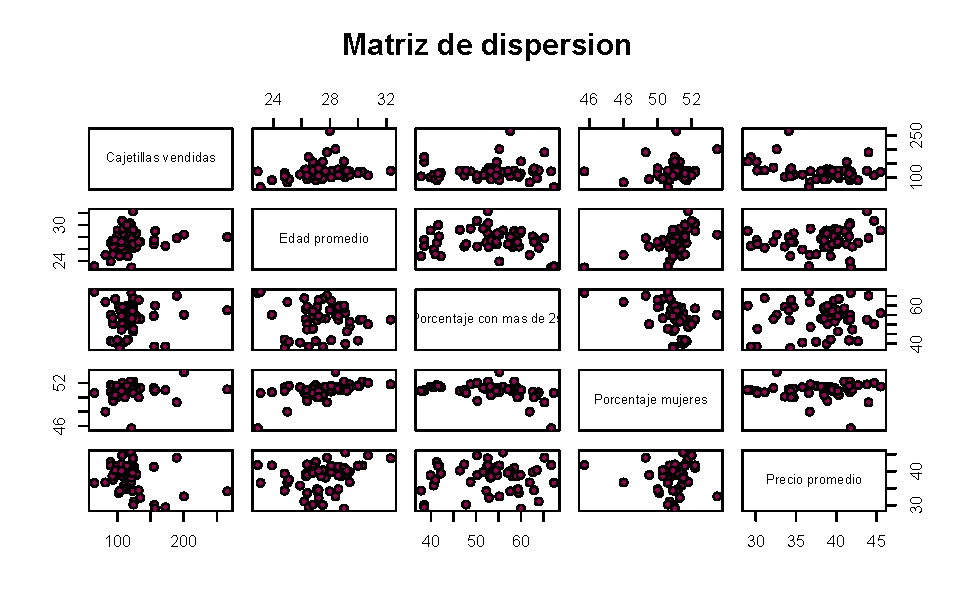
\includegraphics{_main_files/figure-latex/unnamed-chunk-67-1} \end{center}

A simple vista ``no estamos apreciando toda la información'', haremos gráficos dos a dos:

\begin{Shaded}
\begin{Highlighting}[]
\FunctionTok{plot}\NormalTok{(cigarros}\SpecialCharTok{$}\NormalTok{AGE,cigarros}\SpecialCharTok{$}\NormalTok{SCIG,}\AttributeTok{type =} \StringTok{"p"}\NormalTok{,}\AttributeTok{col=}\StringTok{"deeppink4"}\NormalTok{,}\AttributeTok{pch=}\DecValTok{16}\NormalTok{,}
\AttributeTok{xlab=}\StringTok{"Edad promedio"}\NormalTok{, }\AttributeTok{ylab=}\StringTok{"Cajetillas vendidas"}\NormalTok{,}
\AttributeTok{main=} \StringTok{"Relación entre la edad promedio y las cajetillas vendidas"}\NormalTok{)}
\end{Highlighting}
\end{Shaded}

\begin{center}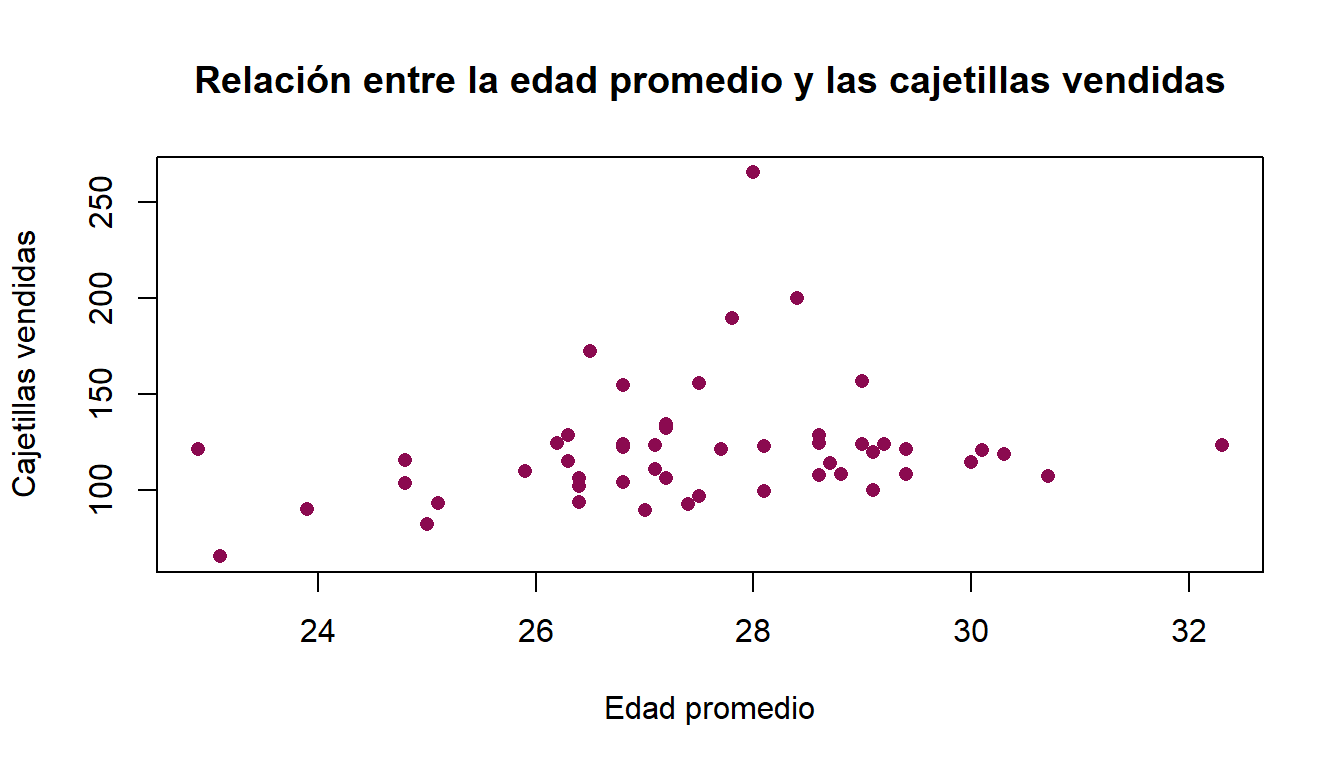
\includegraphics{_main_files/figure-latex/unnamed-chunk-68-1} \end{center}

\begin{Shaded}
\begin{Highlighting}[]
\FunctionTok{plot}\NormalTok{(cigarros}\SpecialCharTok{$}\NormalTok{ED,cigarros}\SpecialCharTok{$}\NormalTok{SCIG,}\AttributeTok{type =} \StringTok{"p"}\NormalTok{,}\AttributeTok{col=}\StringTok{"deeppink4"}\NormalTok{,}\AttributeTok{pch=}\DecValTok{16}\NormalTok{,}
\AttributeTok{xlab=}\StringTok{"Porcentaje con más de 25"}\NormalTok{, }\AttributeTok{ylab=}\StringTok{"Cajetillas vendidas"}\NormalTok{,}
\AttributeTok{main=} \StringTok{"Relación entre el porcentaje con más de 25 y las cajetillas vendidas"}\NormalTok{)}
\end{Highlighting}
\end{Shaded}

\begin{center}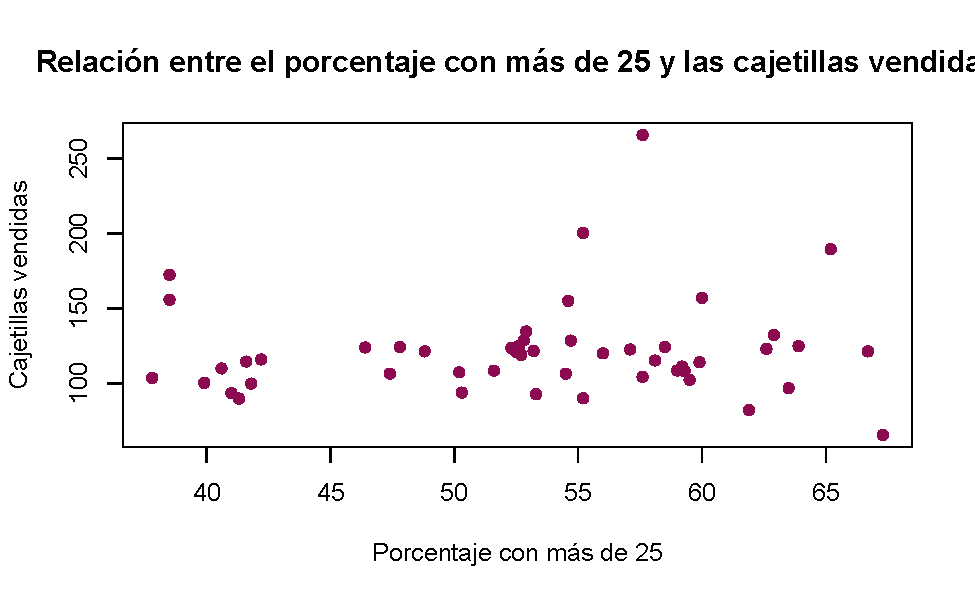
\includegraphics{_main_files/figure-latex/unnamed-chunk-69-1} \end{center}

\begin{Shaded}
\begin{Highlighting}[]
\FunctionTok{plot}\NormalTok{(cigarros}\SpecialCharTok{$}\NormalTok{PERFEM,cigarros}\SpecialCharTok{$}\NormalTok{SCIG,}\AttributeTok{type =} \StringTok{"p"}\NormalTok{,}\AttributeTok{col=}\StringTok{"deeppink4"}\NormalTok{,}\AttributeTok{pch=}\DecValTok{16}\NormalTok{,}
\AttributeTok{xlab=}\StringTok{"Porcentaje de mujeres"}\NormalTok{, }\AttributeTok{ylab=}\StringTok{"Cajetillas vendidas"}\NormalTok{,}
\AttributeTok{main=} \StringTok{"Relación entre el porcentaje de mujeres y las cajetillas vendidas"}\NormalTok{)}
\end{Highlighting}
\end{Shaded}

\begin{center}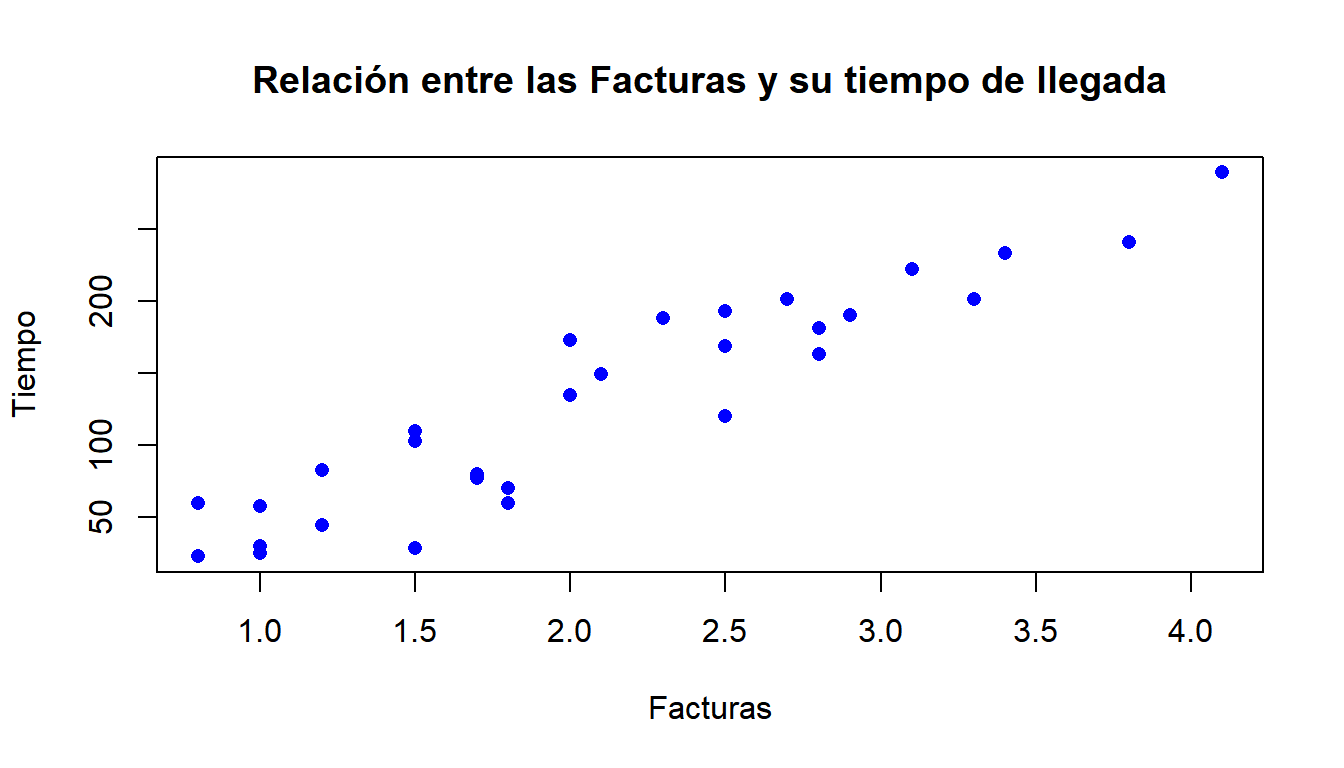
\includegraphics{_main_files/figure-latex/unnamed-chunk-70-1} \end{center}

\begin{Shaded}
\begin{Highlighting}[]
\FunctionTok{plot}\NormalTok{(cigarros}\SpecialCharTok{$}\NormalTok{PRICE,cigarros}\SpecialCharTok{$}\NormalTok{SCIG,}\AttributeTok{type =} \StringTok{"p"}\NormalTok{,}\AttributeTok{col=}\StringTok{"deeppink4"}\NormalTok{,}\AttributeTok{pch=}\DecValTok{16}\NormalTok{,}
\AttributeTok{xlab=}\StringTok{"Precio"}\NormalTok{, }\AttributeTok{ylab=}\StringTok{"Cajetillas vendidas"}\NormalTok{,}
\AttributeTok{main=} \StringTok{"Relación entre el precio y las cajetillas vendidas"}\NormalTok{)}
\end{Highlighting}
\end{Shaded}

\begin{center}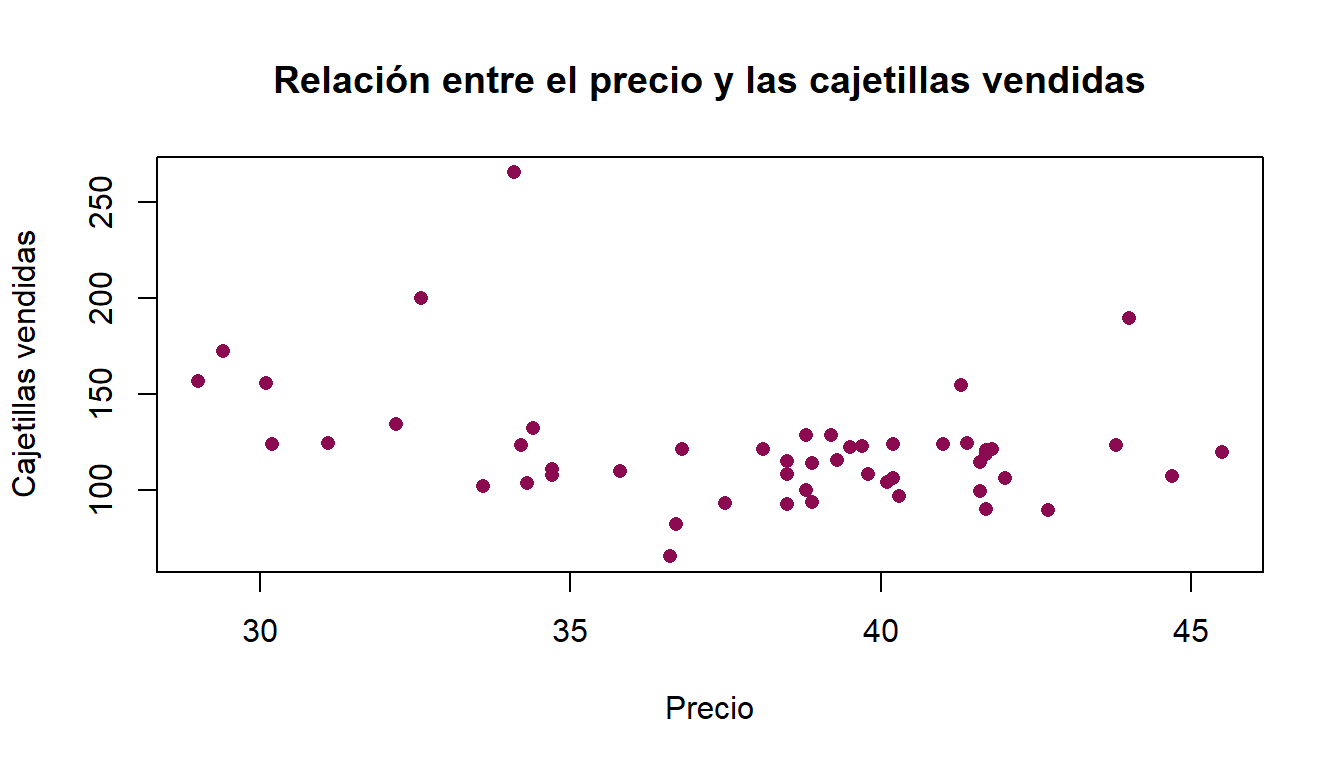
\includegraphics{_main_files/figure-latex/unnamed-chunk-71-1} \end{center}

Observemos que tanto la variable de promedio de más de 25 y las cajetillas vendidas muestran una relación, al igual que la variable precio.

Veamos ahora la correlación entre las variables:

\begin{Shaded}
\begin{Highlighting}[]
\FunctionTok{cor}\NormalTok{(cigarros)}
\end{Highlighting}
\end{Shaded}

\begin{verbatim}
             ESTADO        SCIG         AGE          ED       PERFEM
ESTADO  1.000000000 -0.11088992  0.05535895 -0.05138058 -0.002021391
SCIG   -0.110889919  1.00000000  0.21500813  0.05494773  0.142960829
AGE     0.055358955  0.21500813  1.00000000 -0.12564933  0.555087298
ED     -0.051380577  0.05494773 -0.12564933  1.00000000 -0.434958738
PERFEM -0.002021391  0.14296083  0.55508730 -0.43495874  1.000000000
PRICE  -0.055232952 -0.30696253  0.26605603  0.04667213  0.049060568
             PRICE
ESTADO -0.05523295
SCIG   -0.30696253
AGE     0.26605603
ED      0.04667213
PERFEM  0.04906057
PRICE   1.00000000
\end{verbatim}

Las correlaciones entre las variables que no son las cajetillas vendidas no son ``altas'' por lo que en principio no parece haber problema de considerar todas las variables dentro del modelo.

\textbf{Segundo Paso: Generación de Modelos y Elección del Mejor Modelo}

Emplearemos comandos de R:

Empezaremos con el modelo inicial, le llamamos así ya que es el modelo más grande que podemos suponer, ya que el modelo explica las cajetillas vendidas en función de las otras 4 variables:

\begin{Shaded}
\begin{Highlighting}[]
\NormalTok{modeloini}\OtherTok{=}\FunctionTok{lm}\NormalTok{(SCIG}\SpecialCharTok{\textasciitilde{}}\NormalTok{AGE}\SpecialCharTok{+}\NormalTok{ED}\SpecialCharTok{+}\NormalTok{PERFEM}\SpecialCharTok{+}\NormalTok{PRICE, }\AttributeTok{data=}\NormalTok{cigarros) }
\FunctionTok{summary}\NormalTok{(modeloini)}
\end{Highlighting}
\end{Shaded}

\begin{verbatim}

Call:
lm(formula = SCIG ~ AGE + ED + PERFEM + PRICE, data = cigarros)

Residuals:
    Min      1Q  Median      3Q     Max 
-43.242 -13.160  -5.053   3.166 128.099 

Coefficients:
            Estimate Std. Error t value Pr(>|t|)   
(Intercept)  -8.0742   231.4589  -0.035  0.97231   
AGE           5.2521     2.6733   1.965  0.05492 . 
ED            0.5115     0.5389   0.949  0.34699   
PERFEM        1.3716     4.8326   0.284  0.77770   
PRICE        -2.9599     0.9713  -3.047  0.00365 **
---
Signif. codes:  0 '***' 0.001 '**' 0.01 '*' 0.05 '.' 0.1 ' ' 1

Residual standard error: 28.62 on 51 degrees of freedom
Multiple R-squared:  0.2034,    Adjusted R-squared:  0.1409 
F-statistic: 3.255 on 4 and 51 DF,  p-value: 0.01878
\end{verbatim}

De este primer modelo dado que las pruebas de hipótesis para cada \(\beta_{i}\) nos dicen que la única variable significativa es \(\beta_{4}\) que es para la variable Precio. Y hasta el momento tiene sentido esto.

Ahora si, emplearemos el método backward con el criterio AIC.

\begin{Shaded}
\begin{Highlighting}[]
\NormalTok{modelo\_backward\_AIC}\OtherTok{=}\FunctionTok{stepAIC}\NormalTok{(modeloini,}\AttributeTok{direction =} \StringTok{"backward"}\NormalTok{)}
\end{Highlighting}
\end{Shaded}

\begin{verbatim}
Start:  AIC=380.41
SCIG ~ AGE + ED + PERFEM + PRICE

         Df Sum of Sq   RSS    AIC
- PERFEM  1      66.0 41828 378.49
- ED      1     737.8 42500 379.39
<none>                41762 380.41
- AGE     1    3160.6 44923 382.49
- PRICE   1    7604.1 49366 387.77

Step:  AIC=378.49
SCIG ~ AGE + ED + PRICE

        Df Sum of Sq   RSS    AIC
- ED     1     689.2 42517 377.41
<none>               41828 378.49
- AGE    1    5402.7 47231 383.30
- PRICE  1    7813.1 49641 386.08

Step:  AIC=377.41
SCIG ~ AGE + PRICE

        Df Sum of Sq   RSS    AIC
<none>               42517 377.41
- AGE    1    4965.6 47483 381.60
- PRICE  1    7481.7 49999 384.49
\end{verbatim}

Ahora observemos el mejor modelo, de acuerdo a lo arrojado en \textbf{stepAIC()}.

\begin{Shaded}
\begin{Highlighting}[]
\FunctionTok{summary}\NormalTok{(modelo\_backward\_AIC)}
\end{Highlighting}
\end{Shaded}

\begin{verbatim}

Call:
lm(formula = SCIG ~ AGE + PRICE, data = cigarros)

Residuals:
    Min      1Q  Median      3Q     Max 
-35.828 -15.601  -6.451   3.807 130.691 

Coefficients:
            Estimate Std. Error t value Pr(>|t|)   
(Intercept)  83.4541    61.0443   1.367  0.17736   
AGE           5.3878     2.1656   2.488  0.01603 * 
PRICE        -2.9121     0.9536  -3.054  0.00353 **
---
Signif. codes:  0 '***' 0.001 '**' 0.01 '*' 0.05 '.' 0.1 ' ' 1

Residual standard error: 28.32 on 53 degrees of freedom
Multiple R-squared:  0.1889,    Adjusted R-squared:  0.1583 
F-statistic: 6.174 on 2 and 53 DF,  p-value: 0.003889
\end{verbatim}

A través de la tablas ANOVA se tiene:

\begin{Shaded}
\begin{Highlighting}[]
\FunctionTok{anova}\NormalTok{(modelo\_backward\_AIC)}
\end{Highlighting}
\end{Shaded}

\begin{verbatim}
Analysis of Variance Table

Response: SCIG
          Df Sum Sq Mean Sq F value   Pr(>F)   
AGE        1   2423  2423.4  3.0209 0.088005 . 
PRICE      1   7482  7481.7  9.3264 0.003529 **
Residuals 53  42517   802.2                    
---
Signif. codes:  0 '***' 0.001 '**' 0.01 '*' 0.05 '.' 0.1 ' ' 1
\end{verbatim}

De los resultados obtenidos podemos refinar el \(mejor \ modelo\) obtenido:

\begin{Shaded}
\begin{Highlighting}[]
\NormalTok{modelo\_refinado}\OtherTok{=}\FunctionTok{lm}\NormalTok{(SCIG}\SpecialCharTok{\textasciitilde{}}\DecValTok{0}\SpecialCharTok{+}\NormalTok{AGE}\SpecialCharTok{+}\NormalTok{PRICE,cigarros)}
\FunctionTok{summary}\NormalTok{(modelo\_refinado)}
\end{Highlighting}
\end{Shaded}

\begin{verbatim}

Call:
lm(formula = SCIG ~ 0 + AGE + PRICE, data = cigarros)

Residuals:
    Min      1Q  Median      3Q     Max 
-30.841 -16.734  -5.385   4.999 131.509 

Coefficients:
      Estimate Std. Error t value Pr(>|t|)    
AGE      7.809      1.257   6.214 7.73e-08 ***
PRICE   -2.477      0.906  -2.734  0.00845 ** 
---
Signif. codes:  0 '***' 0.001 '**' 0.01 '*' 0.05 '.' 0.1 ' ' 1

Residual standard error: 28.55 on 54 degrees of freedom
Multiple R-squared:  0.9495,    Adjusted R-squared:  0.9476 
F-statistic: 507.6 on 2 and 54 DF,  p-value: < 2.2e-16
\end{verbatim}

Entonces ya obtuvimos el mejor modelo, que está compuesto por:

\[\mbox{Cajetillas vendidas}= 7.809*\mbox{Edad promedio}-2.477*\mbox{Precio}\]
Bueno todavía debemos validar los supuestos:

\textbf{Tercer Paso Validadción de Supuestos}

Siguiendo el orden de nuestros capítulos, para validar gráficamente la normalidad de los errores debemos graficar los errores contra los cuantiles de la distribución normal.Para ello aplicamos la función \textbf{qqnorm} y con \textbf{qqline} obtenemos la recta diagonal que nos servirá para ver que tan lejos o cerca de la distribución normal están cayendo los residuales.

\begin{Shaded}
\begin{Highlighting}[]
\FunctionTok{qqnorm}\NormalTok{(}\FunctionTok{rstandard}\NormalTok{(modelo\_refinado),}\AttributeTok{ylim =} \FunctionTok{c}\NormalTok{(}\SpecialCharTok{{-}}\DecValTok{2}\NormalTok{,}\DecValTok{2}\NormalTok{),}\AttributeTok{xlim =} \FunctionTok{c}\NormalTok{(}\SpecialCharTok{{-}}\DecValTok{2}\NormalTok{,}\DecValTok{2}\NormalTok{))}
\FunctionTok{qqline}\NormalTok{(}\FunctionTok{rstandard}\NormalTok{(modelo\_refinado),}\AttributeTok{distribution =}\NormalTok{ qnorm,}\AttributeTok{col=}\StringTok{"deeppink4"}\NormalTok{)}
\end{Highlighting}
\end{Shaded}

\begin{center}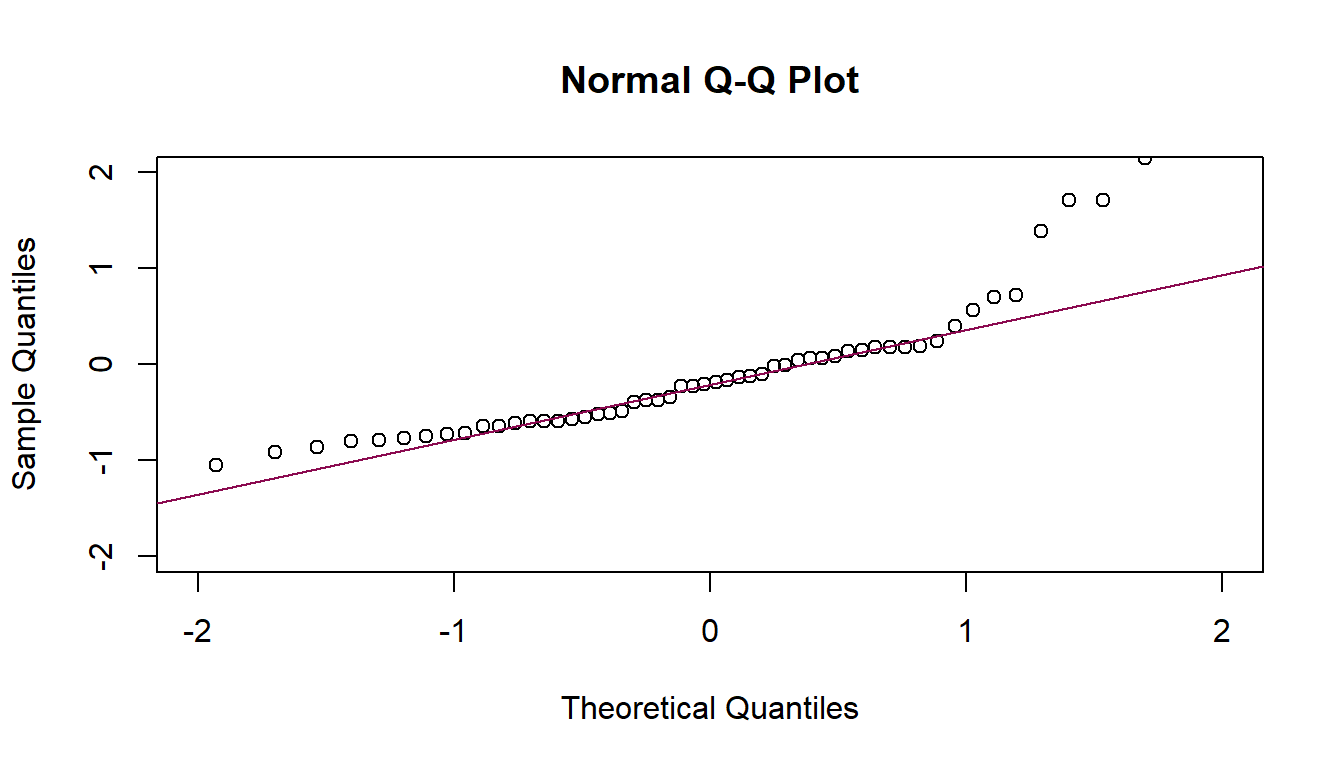
\includegraphics{_main_files/figure-latex/unnamed-chunk-78-1} \end{center}

Podemos observar que la parte central de la distribución si se ajusta a una distribución normal, sin embargo, en los extremos los residuales ya no se comportan como una distribución normal.

Podemos aplicar la prueba de bondad de ajuste \textbf{Lilliefors para normalidad} vista en Bondad de Ajuste:

\begin{Shaded}
\begin{Highlighting}[]
\NormalTok{nortest}\SpecialCharTok{::}\FunctionTok{lillie.test}\NormalTok{(}\FunctionTok{rstandard}\NormalTok{(modelo\_refinado))}
\end{Highlighting}
\end{Shaded}

\begin{verbatim}

    Lilliefors (Kolmogorov-Smirnov) normality test

data:  rstandard(modelo_refinado)
D = 0.23318, p-value = 4.065e-08
\end{verbatim}

Como el valor del \(p-value\) es menor al nivel de significancia \(\alpha=0.05\) entonces rechazamos \(H_{0}\), es decir nuestros residuales no tienen distribución normal.

\textbf{Supuesto de Linealidad}

Como se menciona en el capítulo, graficaremos los errores estandarizados contra los valores observados de la variable explicativa.

\begin{center}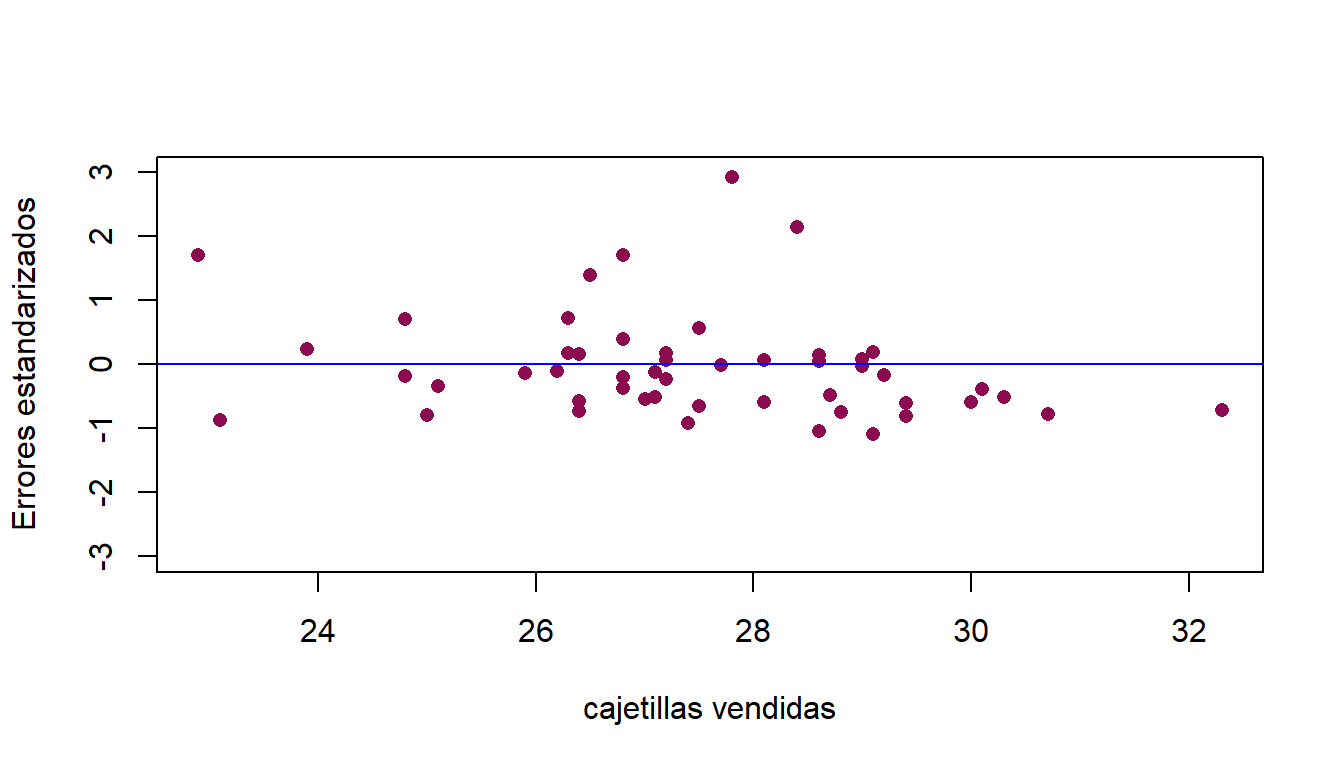
\includegraphics{_main_files/figure-latex/unnamed-chunk-80-1} \end{center}

\begin{center}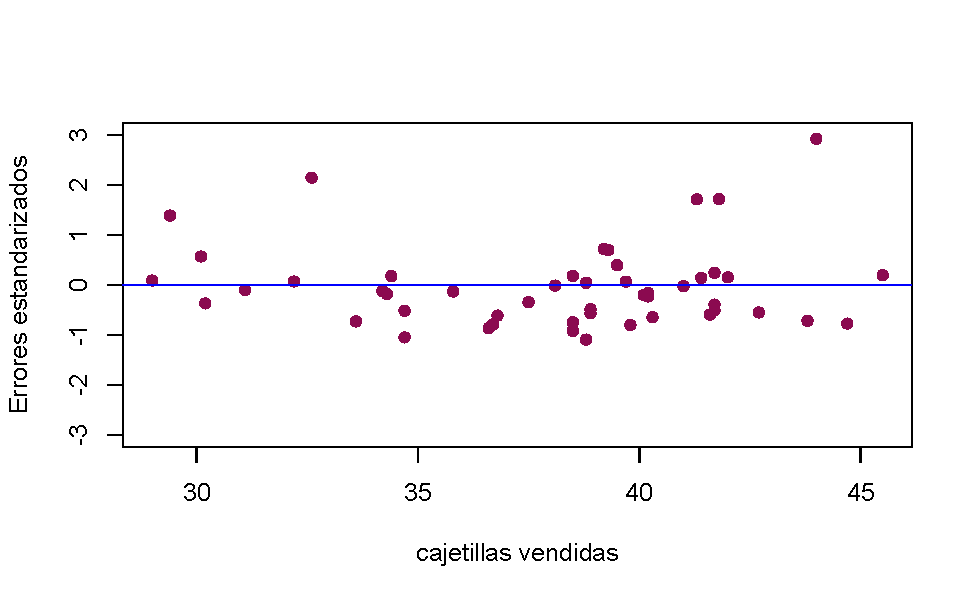
\includegraphics{_main_files/figure-latex/unnamed-chunk-81-1} \end{center}

Para ambas variables, salvo por la posible presencia de algunos valores atípicos que salen de la franja horizontal \((-2,2)\), el resto de las observaciones parecen distribuirse como ruido blanco.

\textbf{Supuesto de Homocedasticidad}

Se dice que una muestra es homocedástica cuando la varianza es constante a lo largo de todas las observaciones, es decir, no varia conforme se presentan nuevas observaciones.

\begin{center}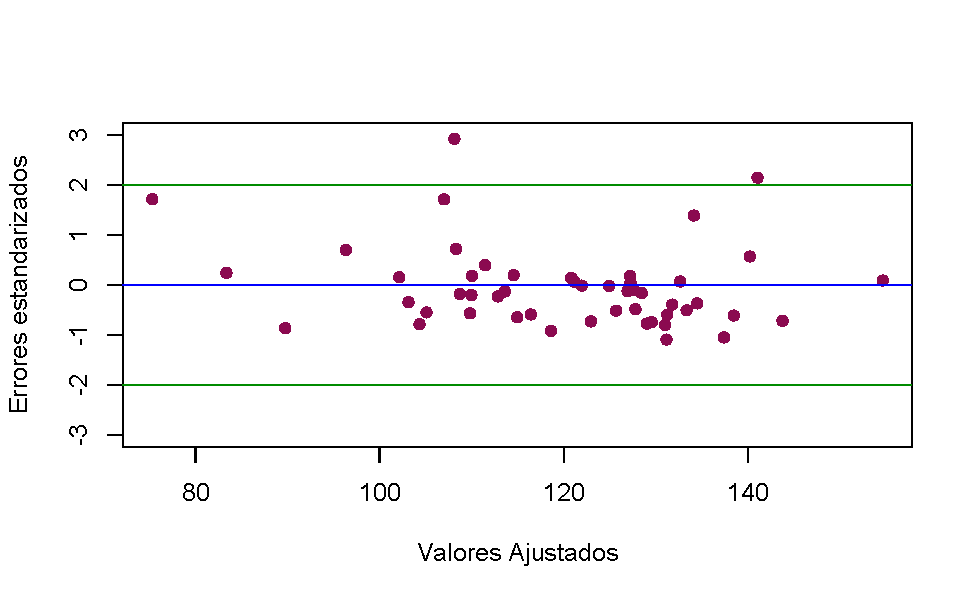
\includegraphics{_main_files/figure-latex/unnamed-chunk-82-1} \end{center}

\begin{itemize}
\tightlist
\item
  Si la varianza es constante entonces la gráfica fluctuaráentre el eje horizontal de manera simétrica, y sin seguir algún patrón, y se espera que la mayor parte de los errores estén contenidos en franjas horizontales delimitados por el eje entre -2 y 2. En éste ejemplo la dispersión regular de los residuales dentro de las Bandas superior e inferior y que no haya residuales que se alejen tanto de la Banda 0, indican varianza constante.
\end{itemize}

Adicionalmente aplicaremos las pruebas vistas en el capítulo para tener certeza estadística de la validez del supuesto de homocedasticidad.

\textbf{Prueba White}

\begin{Shaded}
\begin{Highlighting}[]
\NormalTok{dataset}\OtherTok{=}\FunctionTok{data.frame}\NormalTok{(cigarros}\SpecialCharTok{$}\NormalTok{AGE,cigarros}\SpecialCharTok{$}\NormalTok{PRICE,cigarros}\SpecialCharTok{$}\NormalTok{SCIG)}
\NormalTok{mode1}\OtherTok{=}\FunctionTok{VAR}\NormalTok{(dataset,}\AttributeTok{p=}\DecValTok{1}\NormalTok{)}
\CommentTok{\#whites.htest(mode1)}
\end{Highlighting}
\end{Shaded}

Por el \(p-value\), la hipótesis de homocedasticidad no se rechaza.

\textbf{Supuesto de Multicolinealidad}

\begin{Shaded}
\begin{Highlighting}[]
\NormalTok{X1}\OtherTok{=}\FunctionTok{scale}\NormalTok{(cigarros[,}\SpecialCharTok{{-}}\DecValTok{5}\NormalTok{])}

\NormalTok{A}\OtherTok{=}\FunctionTok{t}\NormalTok{(X1)}\SpecialCharTok{\%*\%}\NormalTok{X1}

\NormalTok{kappa}\OtherTok{=}\FunctionTok{max}\NormalTok{(}\FunctionTok{eigen}\NormalTok{(A)}\SpecialCharTok{$}\NormalTok{values)}\SpecialCharTok{/}\FunctionTok{min}\NormalTok{(}\FunctionTok{eigen}\NormalTok{(A)}\SpecialCharTok{$}\NormalTok{values)}
\NormalTok{kappa}
\end{Highlighting}
\end{Shaded}

\begin{verbatim}
[1] 3.151592
\end{verbatim}

El coeficiente \(kappa\) es de 3.15 por lo tanto no tenemos problemas de multicolinealidad.

\hypertarget{apuxe9ndice}{%
\chapter{Apéndice}\label{apuxe9ndice}}

Será conveniente desarrollar algunas variantes en la forma en la que se denota a los residuales, para ello se define a la matriz \(H\) como \(H=X(X'X)^{-1}X'\),es conocida como \textbf{``matriz sombrero''}, que junto con la matriz \((I-H)\) cumplen con ser matrices idempotentes, es decir, que al elevar las matrices a una potencia dada los valores contenidos en la matriz no se modifican; de igual forma ambas matrices cumplen con ser simétricas, denominadas así ya que al transponer las matrices los valores contenidos en ellas conservan su lugar.

Debemos considerar el siguiente resultado, el cual será importante al desarrollar el siguiente teorema A ya que demuestra que \((X'X)^{-1}\) es una matriz simétrica.

\[[(X'X)^{-1}]'=[(X'X)']^{-1}\]
\[=(X'(X')')^{-1}\]
\[\therefore [(X'X)^{-1}]'= (X'X)^{-1}. \blacksquare\]
Es decir, la inversa de \(X'X\) es simétrica, resultado importante en el siguiente teorema:

\textbf{Teorema A} Sea \(H=X(X'X)^{-1}X'\) e \((I-H)\) entonces:

\textbf{a)} Las matrices \(H\) e \(I-H\) son idempotentes.

\textbf{b)} Las matrices \(H\) e \(I-H\) son simétricas.

\textbf{Demostración:}

\textbf{a)} Para demostrar la idempotencia de \(H\) basta probar que \(H^2=H,\) es decir, al elevar la matriz \(H\) ésta no se alterará:

\[H^2=(X(X'X)^{-1}X')(X(X'X)^{-1}X')\]
\[=X(X'X)^{-1}X'X(X'X)^{-1}X'.\]
Tranponiendo con la finalidad de simplificar el producto matricial y por el resultado mostrado anteriormente \([(X'X)^{-1}]'=(X'X)^{-1}\) se tiene:

\[=[(X'X)^{-1}X'X(X'X)^{-1}X']'X'\]
\[=[(X'X)^{-1}X']'X'\]
\[=X(X'X)^{-1}X'\]

\[\therefore H^2=H.\]
Por lo tanto \(H\) es idempotente. \(\blacksquare\)

Para probar la idempotencia de \(I-H\), ésta será elevada al cuadrado.

\[(I-H)^2=(I-H)(I-H)\]
\[=I-IH-IH+H^2\]
\[=I-2H+H^2.\]

Por idempotencia de \(H\), \(H=H^2\). Por lo tanto:
\[(I-H)=I-2H+H\]
\[\therefore (I-H)^2=I-H.\]

\textbf{b)} Para demostrar la simetría de \(H\), se transpondrá la matriz \(H\). Además debemos recordar que \([(X'X)^{-1}]'=(X'X)^{-1}\) así:

\[H'= (X(X'X)^{-1}X')'\]
\[=X(X'X)^{-1}X'\]
\[\therefore H'= H.\]

Por lo tanto la matriz \(H\) es simétrica.

Para la simetría de \(I-H\) se transpone la matriz:

\[(I-H)'=I'-H'.\]
Por simetría de H y de I

\[\therefore (I-H)^2=I-H\]

Por lo tanto \(I-H\) es simétrica. \(\blacksquare\)

\textbf{Corolario A} Sea \(\underline{e}\) la matriz de residuales entonces estos pueden ser expresados por la siguiente ecuación:

\[\underline{e}=(I-H)\underline{Y}\]
donde \(I\) es la matriz identidad, y \(H=X(X'X)^{-1}X'.\)

\textbf{Demostración:}

Se sabe que los valores estimados son calculados de la siguiente manera:

\[\underline{\hat{Y}}=X\underline{\hat{\beta}}\]
\[\underline{\hat{Y}}=X(X'X)^{-1}X'\underline{Y}\]
\[\underline{\hat{Y}}=H\underline{Y}.\]
donde \(H=X(X'X)^{-1}X'.\) De esta manera calculando la matriz de residuales se tiene:

\[\underline{e}=\underline{Y}-\underline{\hat{Y}}\]
\[\underline{e}=\underline{Y}-X\underline{\hat{\beta}}\]
\[\underline{e}=\underline{Y}-H\underline{Y}\]
\[\underline{e}=(I-H)\underline{Y}.\blacksquare\]

\textbf{Teorema B} Sea una variable de interés \(\underline{Y}\), llamada \textbf{dependiente}, relacionada con dos o más variables explicativas\(x_{1},x_{2},\ldots,x_{k}\),
entonces:

\textbf{a)} \(\mathbf{E}[\underline{Y}]= \beta_{0}+\beta_{1}x_{1}+\beta_{2}x_{2}+ \ldots + \beta_{k}x_{k}.\)

\textbf{b)} \(Var(\underline{Y})= \sigma^2.\)

\textbf{Demostración:}

\textbf{a)} Para la esperanza de \(\underline{Y}\) se tiene:

\[\mathbf{E}[\underline{Y}]=\mathbf{E}[\beta_{0}+\beta_{1}x_{1}+\beta_{2}x_{2}+ \ldots +\beta_{k}x_{k}+\epsilon].\]
La estimación es sobre \(\underline{Y},\)
como \(\beta_{0},\beta_{1},\beta_{2},\ldots,\beta_{k}\) son constantes; \(x_{1},x_{2}, \ldots,x_{k}\) son los valores dados, por lo que:

\[\mathbf{E}[\underline{Y}]=\beta_{0}+\beta_{1}x_{1}+\beta_{2}x_{2}+ \ldots +\beta_{k}x_{k}+\mathbf{E}[\epsilon].\]

\[=\beta_{0}+\beta_{1}x_{1}+\beta_{2}x_{2}+ \ldots +\beta_{k}x_{k}+0\]
\[\therefore \mathbf{E}[\underline{Y}]= \beta_{0}+\beta_{1}x_{1}+\beta_{2}x_{2}+ \ldots + \beta_{k}x_{k}. \blacksquare\]

\textbf{b)} Para la varianza de \(\underline{Y}\) se tiene:

\[Var(\underline{Y})=Var\left( \beta_{0}+\beta_{1}x_{1}+\beta_{2}x_{2}+ \ldots + \beta_{k}x_{k}+ \epsilon\right).\]
La estimación es sobre \(\underline{Y}\), \(\beta_{0},\beta_{1},\beta_{2},\ldots,\beta_{k}\) sons constantes;\(x_{1},x_{2},\ldots,x_{k}\) son valores dados, por lo que cumple que:

\[Var(\underline{Y})=0+0+0+\ldots+0+Var(\epsilon)\]
\[\therefore Var(\underline{Y})=\sigma^2.\blacksquare\]

\hypertarget{ejemplo-de-regresiuxf3n-lineal-muxfaltiple}{%
\chapter{Ejemplo de regresión lineal múltiple}\label{ejemplo-de-regresiuxf3n-lineal-muxfaltiple}}

Ahora retomaremos el ejemplo desarrollado en la sección de regresión lineal simple para resolver el problema ajustando un modelo de regresión lineal multiple.

\hypertarget{contexto-del-problema-1}{%
\section{Contexto del problema}\label{contexto-del-problema-1}}

Para esta tarea usaremos los datos almacenados \href{https://raw.githubusercontent.com/alberto-mateos-mo/seminario-est-fciencias/master/datos/linear_regression_data/mmm_Rexample.csv}{aquí}.

Estos datos contienen información sobre el impacto que han tenido diferentes inversiones de publicidad en las ventas de la compañía.

El objetivo de la empresa es entender cómo influyen las diferentes inversiones en publicidad en las ventas.

\hypertarget{exploraciuxf3n-de-datos-1}{%
\section{Exploración de datos}\label{exploraciuxf3n-de-datos-1}}

Para leer los datos directamente de GitHub usaremos la librería \texttt{readr}, la cual puede instalarse usando \texttt{install.packages("readr")}.

\begin{Shaded}
\begin{Highlighting}[]
\FunctionTok{library}\NormalTok{(readr)}
\FunctionTok{library}\NormalTok{(dplyr)}

\NormalTok{datos }\OtherTok{\textless{}{-}} \FunctionTok{read\_csv}\NormalTok{(}\StringTok{"https://raw.githubusercontent.com/alberto{-}mateos{-}mo/seminario{-}est{-}fciencias/master/datos/linear\_regression\_data/mmm\_Rexample.csv"}\NormalTok{)}

\FunctionTok{head}\NormalTok{(datos)}
\end{Highlighting}
\end{Shaded}

\begin{verbatim}
# A tibble: 6 x 5
  index    tv social_networks   ooh sales
  <dbl> <dbl>           <dbl> <dbl> <dbl>
1     1 230.             37.8  69.2  2210
2     2  44.5            39.3  45.1  1040
3     3  17.2            45.9  69.3   930
4     4 152.             41.3  58.5  1850
5     5 181.             10.8  58.4  1290
6     6   8.7            48.9  75     720
\end{verbatim}

Como podemos ver tenemos información de las ventas de la compañía y de los montos que se han destinado para publicidad en televisión (tv), redes sociales (social\_networks) y exteriores (ooh).

\hypertarget{visualizaciuxf3n-de-datos-1}{%
\section{Visualización de datos}\label{visualizaciuxf3n-de-datos-1}}

A diferencia del caso de regresión lineal simple, no podemos crear un gráfico de dispersión pues requeriríamos de un espacio de 5 dimensiones para intentar detectar una relación lineal entre las inversiones y las ventas.

Si bien podríamos crear gráficos de dispersión entre cada variable independientes y las ventas, esta tarea podría ser muy lara y poco productiva en conjuntos de datos de alta dimension.

Para tener un vistazo de toda la información al mismo tiempo podemos usar un gráfico de correlaciones.

\begin{Shaded}
\begin{Highlighting}[]
\FunctionTok{library}\NormalTok{(corrplot)}

\NormalTok{datos }\OtherTok{\textless{}{-}}\NormalTok{ datos }\SpecialCharTok{\%\textgreater{}\%} 
\NormalTok{  dplyr}\SpecialCharTok{::}\FunctionTok{select}\NormalTok{(}\SpecialCharTok{{-}}\NormalTok{index)}

\FunctionTok{corrplot}\NormalTok{(}\FunctionTok{cor}\NormalTok{(datos), }\AttributeTok{method =} \StringTok{"number"}\NormalTok{)}
\end{Highlighting}
\end{Shaded}

\begin{center}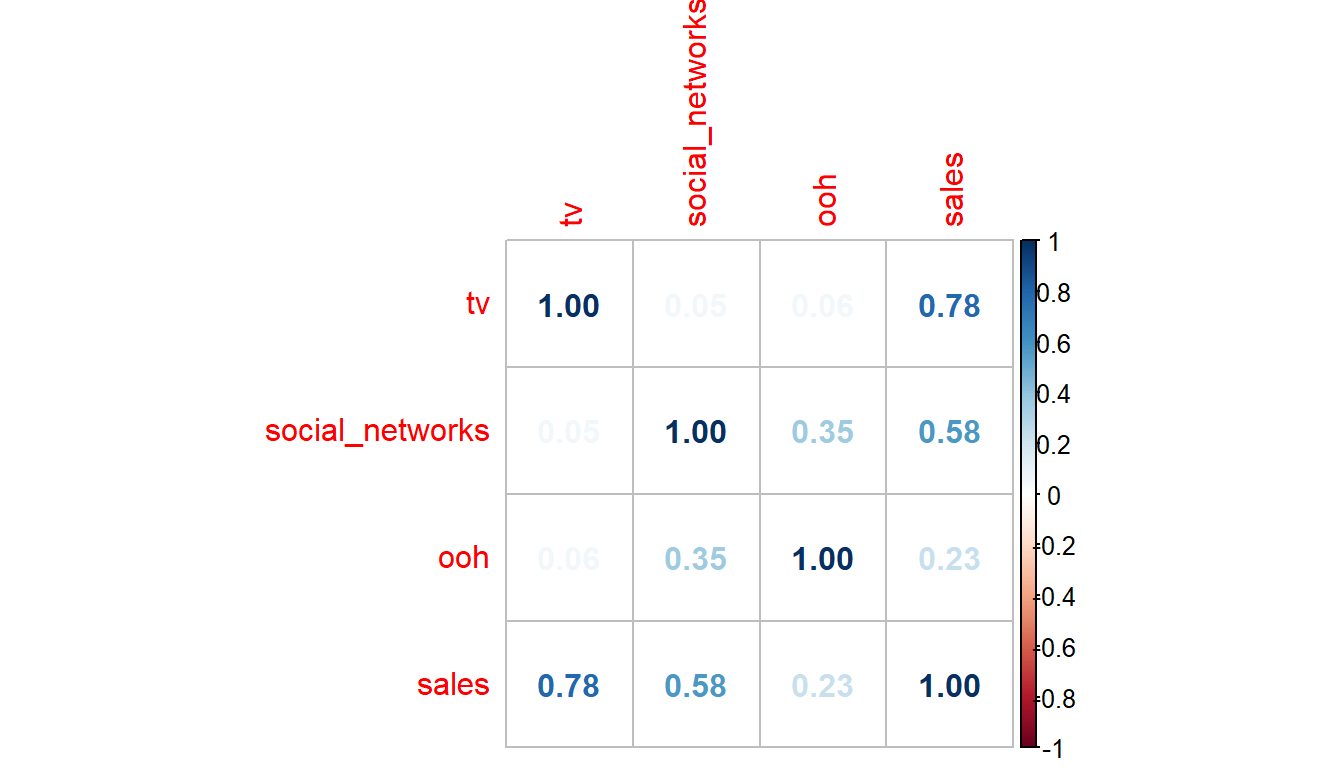
\includegraphics{_main_files/figure-latex/unnamed-chunk-86-1} \end{center}

Además de la relación directa entre tv y ventas también podemos identificar una posible relación entre redes sociales y ventas, con un coeficiente de correlación de 0.58

La correlación entre publicidad exterior (ooh) y ventas es baja (0.23), con lo que podríamos intuir que estas inversiones podrían no ser influyentes en las ventas.

\hypertarget{ajuste-del-modelo-de-regresiuxf3n-lineal-muxfaltiple}{%
\section{Ajuste del modelo de regresión lineal múltiple}\label{ajuste-del-modelo-de-regresiuxf3n-lineal-muxfaltiple}}

Con este modelo encontraremos la ecuación del hiperplano que mejor describa la relación entre nuestras variables de interés.

En el caso multivariado este hiperplano estará descrito de la siguiente forma:

\[sales = \beta_0 + \beta_1*tv + \beta_2*social\ networks + \beta_3*ooh\]

\begin{Shaded}
\begin{Highlighting}[]
\NormalTok{modelo }\OtherTok{\textless{}{-}} \FunctionTok{lm}\NormalTok{(sales }\SpecialCharTok{\textasciitilde{}}\NormalTok{ ., }\AttributeTok{data =}\NormalTok{ datos)}
\end{Highlighting}
\end{Shaded}

\hypertarget{validaciuxf3n-del-modelo-1}{%
\section{Validación del modelo}\label{validaciuxf3n-del-modelo-1}}

Mediante el resumen del modelo tendremos acceso a todas las métricas necesarias para evaluar qué tan \emph{bueno} es.

\begin{Shaded}
\begin{Highlighting}[]
\FunctionTok{summary}\NormalTok{(modelo)}
\end{Highlighting}
\end{Shaded}

\begin{verbatim}

Call:
lm(formula = sales ~ ., data = datos)

Residuals:
    Min      1Q  Median      3Q     Max 
-882.77  -89.08   24.18  118.93  282.92 

Coefficients:
                Estimate Std. Error t value Pr(>|t|)    
(Intercept)     293.8889    31.1908   9.422   <2e-16 ***
tv                4.5765     0.1395  32.809   <2e-16 ***
social_networks  18.8530     0.8611  21.893   <2e-16 ***
ooh              -0.1037     0.5871  -0.177     0.86    
---
Signif. codes:  0 '***' 0.001 '**' 0.01 '*' 0.05 '.' 0.1 ' ' 1

Residual standard error: 168.6 on 196 degrees of freedom
Multiple R-squared:  0.8972,    Adjusted R-squared:  0.8956 
F-statistic: 570.3 on 3 and 196 DF,  p-value: < 2.2e-16
\end{verbatim}

En primer lugar veremos la sección \textbf{Call}, en esta sección se describe qué modelo se esta ajustando; esta parte es meramente informativa.

La sección \textbf{Residuals} nos da una idea de la distribución de los residuales.

\textbf{Para pensar: ¿por qué el resumen del modelo omite la media de los residuales?, ¿qué deberíamos esperar de la mediana?}

\hypertarget{coefficients-1}{%
\subsection{Coefficients}\label{coefficients-1}}

En la tabla de esta sección se muestran:

\begin{itemize}
\item
  Los estimadores de los coeficientes del modelo i.e.~\(\beta_0\) (Intercept), \(\beta_1\) (tv), \(\beta_2\) (social\_networks) y \(\beta_3\) (ooh)
\item
  Los errores estandar para los coeficientes
\item
  El estadístico t y el p-value correspondiente: estos definen la significancia estadística de los estimadores
\end{itemize}

De este ejemplo podemos concluir que el único coeficiente no significativo es el de las inversiones en exteriores, con un p-value de 0.86; es decir, esta varible no es útil para explicar las ventas y podemos excluirla del modelo.

\begin{Shaded}
\begin{Highlighting}[]
\NormalTok{modelo }\OtherTok{\textless{}{-}} \FunctionTok{lm}\NormalTok{(sales }\SpecialCharTok{\textasciitilde{}}\NormalTok{ tv }\SpecialCharTok{+}\NormalTok{ social\_networks, }\AttributeTok{data =}\NormalTok{ datos)}

\FunctionTok{summary}\NormalTok{(modelo)}
\end{Highlighting}
\end{Shaded}

\begin{verbatim}

Call:
lm(formula = sales ~ tv + social_networks, data = datos)

Residuals:
    Min      1Q  Median      3Q     Max 
-879.77  -87.52   24.22  117.08  283.28 

Coefficients:
                Estimate Std. Error t value Pr(>|t|)    
(Intercept)      292.110     29.449   9.919   <2e-16 ***
tv                 4.575      0.139  32.909   <2e-16 ***
social_networks   18.799      0.804  23.382   <2e-16 ***
---
Signif. codes:  0 '***' 0.001 '**' 0.01 '*' 0.05 '.' 0.1 ' ' 1

Residual standard error: 168.1 on 197 degrees of freedom
Multiple R-squared:  0.8972,    Adjusted R-squared:  0.8962 
F-statistic: 859.6 on 2 and 197 DF,  p-value: < 2.2e-16
\end{verbatim}

En el modelo reducido podemos observar que todos los coeficientes son sinificativos, podemos decir que este es el mejor modelo para explicar las ventas de la compañía.

\hypertarget{bondad-de-ajuste-1}{%
\section{Bondad de ajuste}\label{bondad-de-ajuste-1}}

La última sección nos muestra:

\begin{itemize}
\item
  El error estándar de los residuales: representa las variaciones de los datos reales en torno a la linea de regresión ajustada por el modelo.
\item
  R cuadrada y R cuadrada ajustada: representan la proporción de información de los datos que es explicada por el modelo. La diferencia entre ellas es que la R cuadrada ajustada considera en su cálculo una penalización por la cantidad de parámetros que estima el modelo.
\item
  Estadístico F: evalua si al menos una variable independiente tiene coeficiente distinto de cero; es decir resume globalmente si el modelo ajustado es un modelo significativo.
\end{itemize}

\hypertarget{intepretaciuxf3n-de-resultados-1}{%
\section{Intepretación de resultados}\label{intepretaciuxf3n-de-resultados-1}}

Una vez validado el modelo de regresión lineal multiple podemos usar sus resultados para intepretarlos en el contexto del problema.

Recordemos que nuestro objetivo es entender cómo influyen las diferentes inversiones en publicidad en las ventas.

En primer lugar podemos determinar que las inversiones en publicidad por televisión y redes sociales influyen en el desempeño de las ventas.

El coeficiente \(\beta_0\) (Intercept) nos indica las ventas promedio generadas por otros factores no medidos y con inversiones nulas en TV y redes sociales.

El coeficiente \(\beta_1\) asociado a las inversiones en TV nos da el incremento (dado que es positivo) promedio en ventas por cada incremento de una unidad monetaria en TV dado un mismo valor de inversión en redes sociales.

El coeficiente \(\beta_2\) asociado a las inversiones en redes sociales nos da el incremento (dado que es positivo) promedio en ventas por cada incremento de una unidad monetaria en redes sociales dado un mismo valor de inversión en TV.

Es decir:

\begin{itemize}
\item
  Las inversiones en publicidad por TV benefician a las ventas, generando en promedio 4.6 unidades monetarias de venta por cada unidad monetaria invertida en este medio, \emph{ceteris paribus}.
\item
  Las inversiones en publicidad por redes sociales también benefician a las ventas,generando en promedio 18.8 unidades monetarias de venta por cada unidad monetaria invertida en este medio, \emph{ceteris paribus}.
\end{itemize}

Podemos agregar que de las dos inversiones usadas en el modelo, la de redes sociales es más eficiente pues genera un mayor impacto en las ventas.

  \bibliography{book.bib,packages.bib}

\end{document}
